\documentclass[twoside]{book}

% Packages required by doxygen
\usepackage{calc}
\usepackage{doxygen}
\usepackage{graphicx}
\usepackage[utf8]{inputenc}
\usepackage{makeidx}
\usepackage{multicol}
\usepackage{multirow}
\usepackage{textcomp}
\usepackage[table]{xcolor}

% Font selection
\usepackage[T1]{fontenc}
\usepackage{mathptmx}
\usepackage[scaled=.90]{helvet}
\usepackage{courier}
\usepackage{amssymb}
\usepackage{sectsty}
\renewcommand{\familydefault}{\sfdefault}
\allsectionsfont{%
  \fontseries{bc}\selectfont%
  \color{darkgray}%
}
\renewcommand{\DoxyLabelFont}{%
  \fontseries{bc}\selectfont%
  \color{darkgray}%
}

% Page & text layout
\usepackage{geometry}
\geometry{%
  a4paper,%
  top=2.5cm,%
  bottom=2.5cm,%
  left=2.5cm,%
  right=2.5cm%
}
\tolerance=750
\hfuzz=15pt
\hbadness=750
\setlength{\emergencystretch}{15pt}
\setlength{\parindent}{0cm}
\setlength{\parskip}{0.2cm}
\makeatletter
\renewcommand{\paragraph}{%
  \@startsection{paragraph}{4}{0ex}{-1.0ex}{1.0ex}{%
    \normalfont\normalsize\bfseries\SS@parafont%
  }%
}
\renewcommand{\subparagraph}{%
  \@startsection{subparagraph}{5}{0ex}{-1.0ex}{1.0ex}{%
    \normalfont\normalsize\bfseries\SS@subparafont%
  }%
}
\makeatother

% Headers & footers
\usepackage{fancyhdr}
\pagestyle{fancyplain}
\fancyhead[LE]{\fancyplain{}{\bfseries\thepage}}
\fancyhead[CE]{\fancyplain{}{}}
\fancyhead[RE]{\fancyplain{}{\bfseries\leftmark}}
\fancyhead[LO]{\fancyplain{}{\bfseries\rightmark}}
\fancyhead[CO]{\fancyplain{}{}}
\fancyhead[RO]{\fancyplain{}{\bfseries\thepage}}
\fancyfoot[LE]{\fancyplain{}{}}
\fancyfoot[CE]{\fancyplain{}{}}
\fancyfoot[RE]{\fancyplain{}{\bfseries\scriptsize Generated on Fri Feb 17 2017 11\-:06\-:18 for Sarafun Behavior Trees package by Doxygen }}
\fancyfoot[LO]{\fancyplain{}{\bfseries\scriptsize Generated on Fri Feb 17 2017 11\-:06\-:18 for Sarafun Behavior Trees package by Doxygen }}
\fancyfoot[CO]{\fancyplain{}{}}
\fancyfoot[RO]{\fancyplain{}{}}
\renewcommand{\footrulewidth}{0.4pt}
\renewcommand{\chaptermark}[1]{%
  \markboth{#1}{}%
}
\renewcommand{\sectionmark}[1]{%
  \markright{\thesection\ #1}%
}

% Indices & bibliography
\usepackage{natbib}
\usepackage[titles]{tocloft}
\setcounter{tocdepth}{3}
\setcounter{secnumdepth}{5}
\makeindex

% Hyperlinks (required, but should be loaded last)
\usepackage{ifpdf}
\ifpdf
  \usepackage[pdftex,pagebackref=true]{hyperref}
\else
  \usepackage[ps2pdf,pagebackref=true]{hyperref}
\fi
\hypersetup{%
  colorlinks=true,%
  linkcolor=blue,%
  citecolor=blue,%
  unicode%
}

% Custom commands
\newcommand{\clearemptydoublepage}{%
  \newpage{\pagestyle{empty}\cleardoublepage}%
}


%===== C O N T E N T S =====

\begin{document}

% Titlepage & ToC
\hypersetup{pageanchor=false}
\pagenumbering{roman}
\begin{titlepage}
\vspace*{7cm}
\begin{center}%
{\Large Sarafun Behavior Trees package \\[1ex]\large 1 }\\
\vspace*{1cm}
{\large Generated by Doxygen 1.8.6}\\
\vspace*{0.5cm}
{\small Fri Feb 17 2017 11:06:18}\\
\end{center}
\end{titlepage}
\clearemptydoublepage
\tableofcontents
\clearemptydoublepage
\pagenumbering{arabic}
\hypersetup{pageanchor=true}

%--- Begin generated contents ---
\chapter{Main Page}
\label{index}\hypertarget{index}{}This repository contains code that showcases a potential application of behavior trees. It provides\-:
\begin{DoxyItemize}
\item A {\ttfamily sarafun\-\_\-tree} R\-O\-S package. It provides the required utilities for running a behavior tree in the context of the S\-A\-R\-A\-Fun E\-U project.
\item Dummy packages {\ttfamily sarafun\-\_\-manipulation}, {\ttfamily sarafun\-\_\-generic\-\_\-al\-\_\-server} and {\ttfamily sarafun\-\_\-assembly}, that implement \href{http://wiki.ros.org/actionlib}{\tt actionlib} servers for interacting with the behavior tree.
\end{DoxyItemize}

It depends on a modified version of the \href{https://github.com/miccol/ROS-Behavior-Tree}{\tt R\-O\-S-\/\-Behavior-\/\-Tree} package by Michele Colledanchise. The main changes are
\begin{DoxyItemize}
\item Support for the creation of a Behavior Tree from an input file
\item Inclusion of the classes {\ttfamily Action\-Template} and {\ttfamily Condition\-Template}, and their exposure as libraries.
\end{DoxyItemize}

The modified package is found \href{https://github.com/diogoalmeida/ROS-Behavior-Tree}{\tt here}.

\subsection*{Instalation }

\subsubsection*{Compiler}

There is an \href{https://github.com/nlohmann/json/pull/212}{\tt issue} with gcc 4.\-8 that prevents compiling the json parser used in this project. So first, make sure you have a more recent version of gcc. In ubuntu this can be achieved by doing ``` \$ sudo add-\/apt-\/repository ppa\-:ubuntu-\/toolchain-\/r/test \$ sudo apt-\/get update \$ sudo apt-\/get install gcc-\/4.\-9 g++-\/4.9 ``` and your system should now be correctly configured.

\subsubsection*{Dependencies}

The provided packages depend on \href{https://github.com/oftc/yaml-cpp.git}{\tt yaml-\/cpp}.

\subsubsection*{R\-O\-S packages}

If you do not have a created catkin workspace, create one by doing ``` \$ mkdir $\sim$/catkin\-\_\-ws \$ mkdir $\sim$/catkin\-\_\-ws/src \$ cd $\sim$/catkin\-\_\-ws \$ catkin\-\_\-make ``` Otherwise skip this step. Go to the src folder of your catkin workspace and introduce the following commands ``` \$ wstool init \$ wstool merge \href{https://raw.githubusercontent.com/diogoalmeida/sarafun_bt/master/.rosinstall}{\tt https\-://raw.\-githubusercontent.\-com/diogoalmeida/sarafun\-\_\-bt/master/.\-rosinstall} \$ wstool update {\ttfamily  This will download the}R\-O\-S-\/\-Behavior-\/\-Tree{\ttfamily package, as well as the S\-A\-R\-A\-Fun packages required for running the demo. Compile the packages by doing}\$ catkin\-\_\-make -\/\-D\-C\-M\-A\-K\-E\-\_\-\-C\-X\-X\-\_\-\-C\-O\-M\-P\-I\-L\-E\-R=/usr/bin/g++-\/4.9 install{\ttfamily at the root of your workspace. After compiling, do not forget to source the workspace\-: } \$ source devel/setup.\-bash ```

\subsubsection*{Y\-A\-M\-L parser}

These packages depend on yaml-\/cpp, version 0.\-5.\-3, which can be obtained \href{https://github.com/jbeder/yaml-cpp/tree/yaml-cpp-0.5.3}{\tt here}

\subsection*{Services }

The tree client provides services to start, stop and restart a tree. When starting, the tree client will parse the input file and generate a tree based on it. Restarting a tree stops the currently running tree, parses the input file and generates a new one based on it. The provided services are\-:
\begin{DoxyItemize}
\item {\ttfamily /sarafun/start\-\_\-tree}
\item {\ttfamily /sarafun/stop\-\_\-tree}
\item {\ttfamily /sarafun/restart\-\_\-tree}
\end{DoxyItemize}

The start service requires a file path to be given. This will be used by the json parser to load the appropriate tree.

\subsection*{Running the demo }

This package provides two demos\-:
\begin{DoxyItemize}
\item The first demo is used to illustrate the B\-T functionality. It runs the tree defined in {\ttfamily sarafun\-\_\-tree/data/example\-\_\-demo1.\-json}, and each action will prompt the user to enter the key \char`\"{}p\char`\"{} for preempting the action, \char`\"{}a\char`\"{} to abort it and anything else to succeed. Preempting or aborting an action results in a {\ttfamily F\-A\-I\-L\-U\-R\-E} state in the behavior tree. Edit the {\ttfamily sarafun\-\_\-tree/data/example\-\_\-demo1.\-json} file in order to test different tree configurations! To run this demo, type ``` \$ roslaunch sarafun\-\_\-tree run\-\_\-sarafun\-\_\-bt\-\_\-demo.\-launch demo1\-:=true ```
\item The second demo showcases preemption and conditions. We modified the \href{https://github.com/auth-arl/sarafun_online_motion_generation}{\tt online motion generator provided C\-E\-R\-T\-H} so that it implements an actionlib server. The modified code can be found \href{https://github.com/diogoalmeida/sarafun_online_motion_generation}{\tt here} and illustrates how an action should take into account that it can be preempted. To run this demo, type ``` \$ roslaunch sarafun\-\_\-tree run\-\_\-sarafun\-\_\-bt\-\_\-demo.\-launch demo2\-:=true ```
\end{DoxyItemize}

To start execution, call the {\ttfamily /sarafun/start\-\_\-tree} service.

{\bfseries N\-O\-T\-E}\-: The online motion generator requires the {\ttfamily abb\-\_\-irb14000\-\_\-support} package, which is not freely available. You can find the robot description in \href{https://github.com/rtkg/yumi}{\tt this repository}.

This will run a simple tree with 5 actions. Each action will command the robot to move to a different position. The two main subtrees execution depends on the output of the simple condition in the first one. This will be true for the first x ticks on the tree (defined in the launch file under {\ttfamily /\-Is\-Simple/count\-\_\-limit}. When the condition becomes false, the running action will be preempted, and the second subtree is executed, where the first action under the selector asks the robot to achieve an unreachable goal, and is thus preempted after the timeout period has expired.

\subsection*{Creating a different tree }

The behavior tree package takes a json file as input in order to generate the tree. The file is located in {\ttfamily sarafun\-\_\-tree/data} and its name is given by the R\-O\-S parameter {\ttfamily /sarafun/bt/file}. If the parameter is not set, it will use the default name {\ttfamily example.\-json}.

The file defines the tree by specifying its root and a list of nodes. A node can be a flow control node or a leaf node. It is defined by its {\ttfamily id}, {\ttfamily type} and {\ttfamily name} tags and, for the flow control nodes only, by a list of children ({\ttfamily children}) which contains the {\ttfamily id}s of the children nodes. The {\ttfamily id} tag should be unique, and it is used to refer to a particular instance of the behavior tree node. {\ttfamily type} determines the what is the node functionality (see \href{#Currently-supported-node-types}{\tt below}). Finally, the {\ttfamily name} tag is currently only used by the leaf nodes. It specifies the actionlib server name that the concrete action implementation uses and it is used by the behavior tree in order to call the server.

A simple example is as follows ```json \{ \char`\"{}root\char`\"{}\-: \char`\"{}sequence1\char`\"{}, \char`\"{}nodes\char`\"{}\-: \{ \char`\"{}sequence1\char`\"{}\-: \{ \char`\"{}id\char`\"{}\-: \char`\"{}sequence1\char`\"{}, \char`\"{}type\char`\"{}\-: \char`\"{}\-Sequence\-Star\char`\"{}, \char`\"{}name\char`\"{}\-: \char`\"{}\-Sequence\-Star\char`\"{}, \char`\"{}children\char`\"{}\-: \mbox{[} \char`\"{}action1\char`\"{}, \char`\"{}selector1\char`\"{} \mbox{]} \}, \char`\"{}selector1\char`\"{}\-: \{ \char`\"{}id\char`\"{}\-: \char`\"{}selector1\char`\"{}, \char`\"{}type\char`\"{}\-: \char`\"{}\-Selector\char`\"{}, \char`\"{}name\char`\"{}\-: \char`\"{}\-Selector\char`\"{}, \char`\"{}children\char`\"{}\-: \mbox{[} \char`\"{}action2\char`\"{}, \char`\"{}action3\char`\"{} \mbox{]} \}, \char`\"{}action1\char`\"{}\-: \{ \char`\"{}id\char`\"{}\-: \char`\"{}action1\char`\"{}, \char`\"{}type\char`\"{}\-: \char`\"{}\-Action\char`\"{}, \char`\"{}name\char`\"{}\-: \char`\"{}action\-\_\-1\char`\"{} \}, \char`\"{}action2\char`\"{}\-: \{ \char`\"{}id\char`\"{}\-: \char`\"{}action2\char`\"{}, \char`\"{}type\char`\"{}\-: \char`\"{}\-Action\char`\"{}, \char`\"{}name\char`\"{}\-: \char`\"{}action\-\_\-2\char`\"{} \}, \char`\"{}action3\char`\"{}\-: \{ \char`\"{}id\char`\"{}\-: \char`\"{}action3\char`\"{}, \char`\"{}type\char`\"{}\-: \char`\"{}\-Action\char`\"{}, \char`\"{}name\char`\"{}\-: \char`\"{}action\-\_\-3\char`\"{} \} \} \} ```

\subsubsection*{Currently supported node types}

There are four currently supported flow control nodes and two possible leaf node types, which are defined in the json file by the {\ttfamily type} property\-:
\begin{DoxyItemize}
\item {\bfseries Sequence}\-: The sequence node ticks its children sequentially every time it receives a tick from its parent node. Returns {\ttfamily F\-A\-I\-L\-U\-R\-E} as soon as one of its children returns {\ttfamily F\-A\-I\-L\-U\-R\-E}, or {\ttfamily S\-U\-C\-C\-E\-S\-S} in case all of its children are successful
\item {\bfseries Selector}\-: The selector node ticks its children sequentially every time it receives a tick from its parent node. Returns {\ttfamily S\-U\-C\-C\-E\-S\-S} as soon as one of its children returns {\ttfamily S\-U\-C\-C\-E\-S\-S}, or {\ttfamily F\-A\-I\-L\-U\-R\-E} in case all of its children are successful
\item {\bfseries Sequence\-Star}\-: The same as Sequence, but with memory, that is, every time it receives a tick from its parent, it will skip tick'ing all the children that previously returned {\ttfamily S\-U\-C\-C\-E\-S\-S}
\item {\bfseries Selector\-Star}\-: The same as Selector, but with memory, that is, every time it receives a tick from its parent, it will skip tick'ing all the children that previously returned {\ttfamily F\-A\-I\-L\-U\-R\-E}
\item {\bfseries Action}\-: An action will execute some well defined program when it is tick'ed, and will return {\ttfamily S\-U\-C\-C\-E\-S\-S} or {\ttfamily F\-A\-I\-L\-U\-R\-E} at the end of its execution, according to the implementation. While executing, it will return {\ttfamily R\-U\-N\-N\-I\-N\-G}
\item {\bfseries Condition}\-: A condition is similar to an action, but it is meant to return {\ttfamily S\-U\-C\-C\-E\-S\-S} or {\ttfamily F\-A\-I\-L\-U\-R\-E} as soon as it tick'ed, and should be used to help the behavior tree logic by verifying some condition.
\end{DoxyItemize}

\subsection*{Tree visualization }

The B\-T engine provides a basic open\-G\-L tree visualization. An arbitrary tree may not be rendered adequately, in which case the user can use the keyboard to ajust the tree\-:
\begin{DoxyItemize}
\item The directional arrows on the keyboard will translate the tree on the visualization window;
\item Page up will zoom the tree in, page down will zoom out. 
\end{DoxyItemize}
\chapter{Namespace Index}
\section{Namespace List}
Here is a list of all documented namespaces with brief descriptions\-:\begin{DoxyCompactList}
\item\contentsline{section}{\hyperlink{namespacenlohmann}{nlohmann} \\*Namespace for Niels Lohmann }{\pageref{d3/d9b/namespacenlohmann}}{}
\end{DoxyCompactList}

\chapter{Hierarchical Index}
\section{Class Hierarchy}
This inheritance list is sorted roughly, but not completely, alphabetically\-:\begin{DoxyCompactList}
\item Action\-Template\begin{DoxyCompactList}
\item \contentsline{section}{sarafun\-:\-:Execute\-Action$<$ sarafun\-\_\-assembly\-:\-:Folding\-Action, sarafun\-\_\-assembly\-:\-:Folding\-Goal $>$}{\pageref{de/d35/classsarafun_1_1ExecuteAction}}{}
\begin{DoxyCompactList}
\item \contentsline{section}{sarafun\-:\-:Folding\-Assembly\-Action}{\pageref{dd/df2/classsarafun_1_1FoldingAssemblyAction}}{}
\end{DoxyCompactList}
\item \contentsline{section}{sarafun\-:\-:Execute\-Action$<$ sarafun\-\_\-assembly\-:\-:Insertion\-Action, sarafun\-\_\-assembly\-:\-:Insertion\-Goal $>$}{\pageref{de/d35/classsarafun_1_1ExecuteAction}}{}
\begin{DoxyCompactList}
\item \contentsline{section}{sarafun\-:\-:Insertion\-With\-Deformation\-Action}{\pageref{d8/db8/classsarafun_1_1InsertionWithDeformationAction}}{}
\end{DoxyCompactList}
\item \contentsline{section}{sarafun\-:\-:Execute\-Action$<$ sarafun\-\_\-hqp\-\_\-omg\-:\-:Online\-Motion\-Action, sarafun\-\_\-hqp\-\_\-omg\-:\-:Online\-Motion\-Goal $>$}{\pageref{de/d35/classsarafun_1_1ExecuteAction}}{}
\begin{DoxyCompactList}
\item \contentsline{section}{sarafun\-:\-:Online\-Motion\-Action}{\pageref{d0/d3c/classsarafun_1_1OnlineMotionAction}}{}
\end{DoxyCompactList}
\item \contentsline{section}{sarafun\-:\-:Execute\-Action$<$ sarafun\-\_\-manipulation\-:\-:Approach\-Action, sarafun\-\_\-manipulation\-:\-:Approach\-Goal $>$}{\pageref{de/d35/classsarafun_1_1ExecuteAction}}{}
\begin{DoxyCompactList}
\item \contentsline{section}{sarafun\-:\-:Approach\-Objects\-Action}{\pageref{d6/db4/classsarafun_1_1ApproachObjectsAction}}{}
\end{DoxyCompactList}
\item \contentsline{section}{sarafun\-:\-:Execute\-Action$<$ sarafun\-\_\-manipulation\-:\-:Grab\-Action, sarafun\-\_\-manipulation\-:\-:Grab\-Goal $>$}{\pageref{de/d35/classsarafun_1_1ExecuteAction}}{}
\begin{DoxyCompactList}
\item \contentsline{section}{sarafun\-:\-:Grab\-Object\-Action}{\pageref{db/d0c/classsarafun_1_1GrabObjectAction}}{}
\end{DoxyCompactList}
\item \contentsline{section}{sarafun\-:\-:Execute\-Action$<$ sarafun\-\_\-manipulation\-:\-:Place\-Action, sarafun\-\_\-manipulation\-:\-:Place\-Goal $>$}{\pageref{de/d35/classsarafun_1_1ExecuteAction}}{}
\begin{DoxyCompactList}
\item \contentsline{section}{sarafun\-:\-:Place\-Action}{\pageref{d3/dd9/classsarafun_1_1PlaceAction}}{}
\end{DoxyCompactList}
\item \contentsline{section}{sarafun\-:\-:Execute\-Action$<$ sarafun\-\_\-msgs\-:\-:Align\-Keyframe\-Action, sarafun\-\_\-msgs\-:\-:Align\-Keyframe\-Goal $>$}{\pageref{de/d35/classsarafun_1_1ExecuteAction}}{}
\begin{DoxyCompactList}
\item \contentsline{section}{sarafun\-:\-:Align\-Action}{\pageref{dc/df5/classsarafun_1_1AlignAction}}{}
\end{DoxyCompactList}
\item \contentsline{section}{sarafun\-:\-:Execute\-Action$<$ sarafun\-\_\-msgs\-:\-:Assembled\-Keyframe\-Action, sarafun\-\_\-msgs\-:\-:Assembled\-Keyframe\-Goal $>$}{\pageref{de/d35/classsarafun_1_1ExecuteAction}}{}
\begin{DoxyCompactList}
\item \contentsline{section}{sarafun\-:\-:Assembled\-Action}{\pageref{dc/d58/classsarafun_1_1AssembledAction}}{}
\end{DoxyCompactList}
\item \contentsline{section}{sarafun\-:\-:Execute\-Action$<$ sarafun\-\_\-msgs\-:\-:Contact\-Keyframe\-Action, sarafun\-\_\-msgs\-:\-:Contact\-Keyframe\-Goal $>$}{\pageref{de/d35/classsarafun_1_1ExecuteAction}}{}
\begin{DoxyCompactList}
\item \contentsline{section}{sarafun\-:\-:Contact\-Action}{\pageref{dc/d9f/classsarafun_1_1ContactAction}}{}
\end{DoxyCompactList}
\item \contentsline{section}{sarafun\-:\-:Execute\-Action$<$ sarafun\-\_\-msgs\-:\-:Grasp\-Keyframe\-Action, sarafun\-\_\-msgs\-:\-:Grasp\-Keyframe\-Goal $>$}{\pageref{de/d35/classsarafun_1_1ExecuteAction}}{}
\begin{DoxyCompactList}
\item \contentsline{section}{sarafun\-:\-:Grasp\-Action}{\pageref{d0/d03/classsarafun_1_1GraspAction}}{}
\end{DoxyCompactList}
\item \contentsline{section}{sarafun\-:\-:Execute\-Action$<$ sarafun\-\_\-msgs\-:\-:Initial\-Keyframe\-Action, sarafun\-\_\-msgs\-:\-:Initial\-Keyframe\-Goal $>$}{\pageref{de/d35/classsarafun_1_1ExecuteAction}}{}
\begin{DoxyCompactList}
\item \contentsline{section}{sarafun\-:\-:Initial\-Action}{\pageref{d6/d64/classsarafun_1_1InitialAction}}{}
\end{DoxyCompactList}
\item \contentsline{section}{sarafun\-:\-:Execute\-Action$<$ sarafun\-\_\-msgs\-:\-:Move\-Keyframe\-Action, sarafun\-\_\-msgs\-:\-:Move\-Keyframe\-Goal $>$}{\pageref{de/d35/classsarafun_1_1ExecuteAction}}{}
\begin{DoxyCompactList}
\item \contentsline{section}{sarafun\-:\-:Move\-Action}{\pageref{d6/d0e/classsarafun_1_1MoveAction}}{}
\end{DoxyCompactList}
\item \contentsline{section}{sarafun\-:\-:Execute\-Action$<$ sarafun\-\_\-msgs\-:\-:Pick\-Up\-Keyframe\-Action, sarafun\-\_\-msgs\-:\-:Pick\-Up\-Keyframe\-Goal $>$}{\pageref{de/d35/classsarafun_1_1ExecuteAction}}{}
\begin{DoxyCompactList}
\item \contentsline{section}{sarafun\-:\-:Pickup\-Action}{\pageref{d8/dba/classsarafun_1_1PickupAction}}{}
\end{DoxyCompactList}
\item \contentsline{section}{sarafun\-:\-:Execute\-Action$<$ sarafun\-\_\-msgs\-:\-:Retract\-Keyframe\-Action, sarafun\-\_\-msgs\-:\-:Retract\-Keyframe\-Goal $>$}{\pageref{de/d35/classsarafun_1_1ExecuteAction}}{}
\begin{DoxyCompactList}
\item \contentsline{section}{sarafun\-:\-:Retract\-Action}{\pageref{d4/dd3/classsarafun_1_1RetractAction}}{}
\end{DoxyCompactList}
\item \contentsline{section}{sarafun\-:\-:Execute\-Action$<$ Action\-Class, Action\-Goal $>$}{\pageref{de/d35/classsarafun_1_1ExecuteAction}}{}
\end{DoxyCompactList}
\item Condition\-Template\begin{DoxyCompactList}
\item \contentsline{section}{sarafun\-:\-:Is\-Simple}{\pageref{dc/d18/classsarafun_1_1IsSimple}}{}
\end{DoxyCompactList}
\item \contentsline{section}{bt\-\_\-parser\-:\-:Parser}{\pageref{dd/d2f/classbt__parser_1_1Parser}}{}
\item \contentsline{section}{tree\-\_\-generator\-:\-:Sub\-Tree\-From\-K\-F}{\pageref{d9/de6/classtree__generator_1_1SubTreeFromKF}}{}
\item \contentsline{section}{sarafun\-:\-:Test\-Server$<$ Action\-Class, Action\-Goal\-Const\-Ptr, Action\-Feedback, Action\-Result $>$}{\pageref{dd/d24/classsarafun_1_1TestServer}}{}
\item \contentsline{section}{sarafun\-:\-:Test\-Server$<$ sarafun\-\_\-assembly\-:\-:Folding\-Action, sarafun\-\_\-assembly\-:\-:Folding\-Goal\-Const\-Ptr, sarafun\-\_\-assembly\-:\-:Folding\-Feedback, sarafun\-\_\-assembly\-:\-:Folding\-Result $>$}{\pageref{dd/d24/classsarafun_1_1TestServer}}{}
\begin{DoxyCompactList}
\item \contentsline{section}{sarafun\-:\-:Test\-Folding}{\pageref{d3/d6b/classsarafun_1_1TestFolding}}{}
\end{DoxyCompactList}
\item \contentsline{section}{sarafun\-:\-:Test\-Server$<$ sarafun\-\_\-assembly\-:\-:Insertion\-Action, sarafun\-\_\-assembly\-:\-:Insertion\-Goal\-Const\-Ptr, sarafun\-\_\-assembly\-:\-:Insertion\-Feedback, sarafun\-\_\-assembly\-:\-:Insertion\-Result $>$}{\pageref{dd/d24/classsarafun_1_1TestServer}}{}
\begin{DoxyCompactList}
\item \contentsline{section}{sarafun\-:\-:Test\-Insertion}{\pageref{db/ddf/classsarafun_1_1TestInsertion}}{}
\end{DoxyCompactList}
\item \contentsline{section}{sarafun\-:\-:Test\-Server$<$ sarafun\-\_\-manipulation\-:\-:Approach\-Action, sarafun\-\_\-manipulation\-:\-:Approach\-Goal\-Const\-Ptr, sarafun\-\_\-manipulation\-:\-:Approach\-Feedback, sarafun\-\_\-manipulation\-:\-:Approach\-Result $>$}{\pageref{dd/d24/classsarafun_1_1TestServer}}{}
\begin{DoxyCompactList}
\item \contentsline{section}{sarafun\-:\-:Test\-Approach}{\pageref{d7/dfa/classsarafun_1_1TestApproach}}{}
\end{DoxyCompactList}
\item \contentsline{section}{sarafun\-:\-:Test\-Server$<$ sarafun\-\_\-manipulation\-:\-:Grab\-Action, sarafun\-\_\-manipulation\-:\-:Grab\-Goal\-Const\-Ptr, sarafun\-\_\-manipulation\-:\-:Grab\-Feedback, sarafun\-\_\-manipulation\-:\-:Grab\-Result $>$}{\pageref{dd/d24/classsarafun_1_1TestServer}}{}
\begin{DoxyCompactList}
\item \contentsline{section}{sarafun\-:\-:Test\-Grab}{\pageref{de/da2/classsarafun_1_1TestGrab}}{}
\end{DoxyCompactList}
\item \contentsline{section}{sarafun\-:\-:Test\-Server$<$ sarafun\-\_\-manipulation\-:\-:Place\-Action, sarafun\-\_\-manipulation\-:\-:Place\-Goal\-Const\-Ptr, sarafun\-\_\-manipulation\-:\-:Place\-Feedback, sarafun\-\_\-manipulation\-:\-:Place\-Result $>$}{\pageref{dd/d24/classsarafun_1_1TestServer}}{}
\begin{DoxyCompactList}
\item \contentsline{section}{sarafun\-:\-:Test\-Place}{\pageref{db/dff/classsarafun_1_1TestPlace}}{}
\end{DoxyCompactList}
\item \contentsline{section}{sarafun\-:\-:Test\-Server$<$ sarafun\-\_\-msgs\-:\-:Align\-Keyframe\-Action, sarafun\-\_\-msgs\-:\-:Align\-Keyframe\-Goal\-Const\-Ptr, sarafun\-\_\-msgs\-:\-:Align\-Keyframe\-Feedback, sarafun\-\_\-msgs\-:\-:Align\-Keyframe\-Result $>$}{\pageref{dd/d24/classsarafun_1_1TestServer}}{}
\begin{DoxyCompactList}
\item \contentsline{section}{sarafun\-:\-:Test\-Align}{\pageref{d3/d13/classsarafun_1_1TestAlign}}{}
\end{DoxyCompactList}
\item \contentsline{section}{sarafun\-:\-:Test\-Server$<$ sarafun\-\_\-msgs\-:\-:Assembled\-Keyframe\-Action, sarafun\-\_\-msgs\-:\-:Assembled\-Keyframe\-Goal\-Const\-Ptr, sarafun\-\_\-msgs\-:\-:Assembled\-Keyframe\-Feedback, sarafun\-\_\-msgs\-:\-:Assembled\-Keyframe\-Result $>$}{\pageref{dd/d24/classsarafun_1_1TestServer}}{}
\begin{DoxyCompactList}
\item \contentsline{section}{sarafun\-:\-:Test\-Assembled}{\pageref{d1/d63/classsarafun_1_1TestAssembled}}{}
\end{DoxyCompactList}
\item \contentsline{section}{sarafun\-:\-:Test\-Server$<$ sarafun\-\_\-msgs\-:\-:Contact\-Keyframe\-Action, sarafun\-\_\-msgs\-:\-:Contact\-Keyframe\-Goal\-Const\-Ptr, sarafun\-\_\-msgs\-:\-:Contact\-Keyframe\-Feedback, sarafun\-\_\-msgs\-:\-:Contact\-Keyframe\-Result $>$}{\pageref{dd/d24/classsarafun_1_1TestServer}}{}
\begin{DoxyCompactList}
\item \contentsline{section}{sarafun\-:\-:Test\-Contact}{\pageref{dc/d30/classsarafun_1_1TestContact}}{}
\end{DoxyCompactList}
\item \contentsline{section}{sarafun\-:\-:Test\-Server$<$ sarafun\-\_\-msgs\-:\-:Grasp\-Keyframe\-Action, sarafun\-\_\-msgs\-:\-:Grasp\-Keyframe\-Goal\-Const\-Ptr, sarafun\-\_\-msgs\-:\-:Grasp\-Keyframe\-Feedback, sarafun\-\_\-msgs\-:\-:Grasp\-Keyframe\-Result $>$}{\pageref{dd/d24/classsarafun_1_1TestServer}}{}
\begin{DoxyCompactList}
\item \contentsline{section}{sarafun\-:\-:Test\-Grasp}{\pageref{df/d5e/classsarafun_1_1TestGrasp}}{}
\end{DoxyCompactList}
\item \contentsline{section}{sarafun\-:\-:Test\-Server$<$ sarafun\-\_\-msgs\-:\-:Initial\-Keyframe\-Action, sarafun\-\_\-msgs\-:\-:Initial\-Keyframe\-Goal\-Const\-Ptr, sarafun\-\_\-msgs\-:\-:Initial\-Keyframe\-Feedback, sarafun\-\_\-msgs\-:\-:Initial\-Keyframe\-Result $>$}{\pageref{dd/d24/classsarafun_1_1TestServer}}{}
\begin{DoxyCompactList}
\item \contentsline{section}{sarafun\-:\-:Test\-Initial}{\pageref{dd/dba/classsarafun_1_1TestInitial}}{}
\end{DoxyCompactList}
\item \contentsline{section}{sarafun\-:\-:Test\-Server$<$ sarafun\-\_\-msgs\-:\-:Move\-Keyframe\-Action, sarafun\-\_\-msgs\-:\-:Move\-Keyframe\-Goal\-Const\-Ptr, sarafun\-\_\-msgs\-:\-:Move\-Keyframe\-Feedback, sarafun\-\_\-msgs\-:\-:Move\-Keyframe\-Result $>$}{\pageref{dd/d24/classsarafun_1_1TestServer}}{}
\begin{DoxyCompactList}
\item \contentsline{section}{sarafun\-:\-:Test\-Move}{\pageref{d7/dbc/classsarafun_1_1TestMove}}{}
\end{DoxyCompactList}
\item \contentsline{section}{sarafun\-:\-:Test\-Server$<$ sarafun\-\_\-msgs\-:\-:Pick\-Up\-Keyframe\-Action, sarafun\-\_\-msgs\-:\-:Pick\-Up\-Keyframe\-Goal\-Const\-Ptr, sarafun\-\_\-msgs\-:\-:Pick\-Up\-Keyframe\-Feedback, sarafun\-\_\-msgs\-:\-:Pick\-Up\-Keyframe\-Result $>$}{\pageref{dd/d24/classsarafun_1_1TestServer}}{}
\begin{DoxyCompactList}
\item \contentsline{section}{sarafun\-:\-:Test\-Pick\-Up}{\pageref{d6/de5/classsarafun_1_1TestPickUp}}{}
\end{DoxyCompactList}
\item \contentsline{section}{sarafun\-:\-:Test\-Server$<$ sarafun\-\_\-msgs\-:\-:Retract\-Keyframe\-Action, sarafun\-\_\-msgs\-:\-:Retract\-Keyframe\-Goal\-Const\-Ptr, sarafun\-\_\-msgs\-:\-:Retract\-Keyframe\-Feedback, sarafun\-\_\-msgs\-:\-:Retract\-Keyframe\-Result $>$}{\pageref{dd/d24/classsarafun_1_1TestServer}}{}
\begin{DoxyCompactList}
\item \contentsline{section}{sarafun\-:\-:Test\-Retract}{\pageref{d8/db5/classsarafun_1_1TestRetract}}{}
\end{DoxyCompactList}
\item \contentsline{section}{tree\-\_\-generator\-:\-:Tree\-From\-K\-F}{\pageref{d4/de0/classtree__generator_1_1TreeFromKF}}{}
\item \contentsline{section}{sarafun\-:\-:Tree\-Runner}{\pageref{d6/d9c/classsarafun_1_1TreeRunner}}{}
\item \contentsline{section}{tree\-\_\-generator\-:\-:Yaml\-Creator}{\pageref{d4/df1/classtree__generator_1_1YamlCreator}}{}
\end{DoxyCompactList}

\chapter{Data Structure Index}
\section{Class List}
Here are the classes, structs, unions and interfaces with brief descriptions\-:\begin{DoxyCompactList}
\item\contentsline{section}{\hyperlink{classsarafun_1_1AlignAction}{sarafun\-::\-Align\-Action} }{\pageref{classsarafun_1_1AlignAction}}{}
\item\contentsline{section}{\hyperlink{classsarafun_1_1ApproachObjectsAction}{sarafun\-::\-Approach\-Objects\-Action} }{\pageref{classsarafun_1_1ApproachObjectsAction}}{}
\item\contentsline{section}{\hyperlink{classsarafun_1_1AssembledAction}{sarafun\-::\-Assembled\-Action} }{\pageref{classsarafun_1_1AssembledAction}}{}
\item\contentsline{section}{\hyperlink{classnlohmann_1_1basic__json}{nlohmann\-::basic\-\_\-json$<$ Object\-Type, Array\-Type, String\-Type, Boolean\-Type, Number\-Integer\-Type, Number\-Unsigned\-Type, Number\-Float\-Type, Allocator\-Type $>$} \\*Class to store J\-S\-O\-N values }{\pageref{classnlohmann_1_1basic__json}}{}
\item\contentsline{section}{\hyperlink{classnlohmann_1_1basic__json_1_1const__iterator}{nlohmann\-::basic\-\_\-json$<$ Object\-Type, Array\-Type, String\-Type, Boolean\-Type, Number\-Integer\-Type, Number\-Unsigned\-Type, Number\-Float\-Type, Allocator\-Type $>$\-::const\-\_\-iterator} \\*Const random access iterator for the \hyperlink{classnlohmann_1_1basic__json}{basic\-\_\-json} class }{\pageref{classnlohmann_1_1basic__json_1_1const__iterator}}{}
\item\contentsline{section}{\hyperlink{classsarafun_1_1ContactAction}{sarafun\-::\-Contact\-Action} }{\pageref{classsarafun_1_1ContactAction}}{}
\item\contentsline{section}{\hyperlink{classsarafun_1_1ExecuteAction}{sarafun\-::\-Execute\-Action$<$ Action\-Class, Action\-Goal $>$} }{\pageref{classsarafun_1_1ExecuteAction}}{}
\item\contentsline{section}{\hyperlink{classsarafun_1_1FoldingAssemblyAction}{sarafun\-::\-Folding\-Assembly\-Action} }{\pageref{classsarafun_1_1FoldingAssemblyAction}}{}
\item\contentsline{section}{\hyperlink{classsarafun_1_1GrabObjectAction}{sarafun\-::\-Grab\-Object\-Action} }{\pageref{classsarafun_1_1GrabObjectAction}}{}
\item\contentsline{section}{\hyperlink{classsarafun_1_1GraspAction}{sarafun\-::\-Grasp\-Action} }{\pageref{classsarafun_1_1GraspAction}}{}
\item\contentsline{section}{\hyperlink{structstd_1_1hash_3_01nlohmann_1_1json_01_4}{std\-::hash$<$ nlohmann\-::json $>$} \\*Hash value for J\-S\-O\-N objects }{\pageref{structstd_1_1hash_3_01nlohmann_1_1json_01_4}}{}
\item\contentsline{section}{\hyperlink{classsarafun_1_1InitialAction}{sarafun\-::\-Initial\-Action} }{\pageref{classsarafun_1_1InitialAction}}{}
\item\contentsline{section}{\hyperlink{classsarafun_1_1InsertionWithDeformationAction}{sarafun\-::\-Insertion\-With\-Deformation\-Action} }{\pageref{classsarafun_1_1InsertionWithDeformationAction}}{}
\item\contentsline{section}{\hyperlink{classsarafun_1_1IsSimple}{sarafun\-::\-Is\-Simple} }{\pageref{classsarafun_1_1IsSimple}}{}
\item\contentsline{section}{\hyperlink{classnlohmann_1_1basic__json_1_1iterator}{nlohmann\-::basic\-\_\-json$<$ Object\-Type, Array\-Type, String\-Type, Boolean\-Type, Number\-Integer\-Type, Number\-Unsigned\-Type, Number\-Float\-Type, Allocator\-Type $>$\-::iterator} \\*Mutable random access iterator for the \hyperlink{classnlohmann_1_1basic__json}{basic\-\_\-json} class }{\pageref{classnlohmann_1_1basic__json_1_1iterator}}{}
\item\contentsline{section}{\hyperlink{classnlohmann_1_1basic__json_1_1json__pointer}{nlohmann\-::basic\-\_\-json$<$ Object\-Type, Array\-Type, String\-Type, Boolean\-Type, Number\-Integer\-Type, Number\-Unsigned\-Type, Number\-Float\-Type, Allocator\-Type $>$\-::json\-\_\-pointer} \\*J\-S\-O\-N Pointer }{\pageref{classnlohmann_1_1basic__json_1_1json__pointer}}{}
\item\contentsline{section}{\hyperlink{classnlohmann_1_1basic__json_1_1json__reverse__iterator}{nlohmann\-::basic\-\_\-json$<$ Object\-Type, Array\-Type, String\-Type, Boolean\-Type, Number\-Integer\-Type, Number\-Unsigned\-Type, Number\-Float\-Type, Allocator\-Type $>$\-::json\-\_\-reverse\-\_\-iterator$<$ Base $>$} \\*Template for a reverse iterator class }{\pageref{classnlohmann_1_1basic__json_1_1json__reverse__iterator}}{}
\item\contentsline{section}{\hyperlink{classsarafun_1_1MoveAction}{sarafun\-::\-Move\-Action} }{\pageref{classsarafun_1_1MoveAction}}{}
\item\contentsline{section}{\hyperlink{classsarafun_1_1OnlineMotionAction}{sarafun\-::\-Online\-Motion\-Action} }{\pageref{classsarafun_1_1OnlineMotionAction}}{}
\item\contentsline{section}{\hyperlink{classbt__parser_1_1Parser}{bt\-\_\-parser\-::\-Parser} }{\pageref{classbt__parser_1_1Parser}}{}
\item\contentsline{section}{\hyperlink{classsarafun_1_1PickupAction}{sarafun\-::\-Pickup\-Action} }{\pageref{classsarafun_1_1PickupAction}}{}
\item\contentsline{section}{\hyperlink{classsarafun_1_1PlaceAction}{sarafun\-::\-Place\-Action} }{\pageref{classsarafun_1_1PlaceAction}}{}
\item\contentsline{section}{\hyperlink{classsarafun_1_1RetractAction}{sarafun\-::\-Retract\-Action} }{\pageref{classsarafun_1_1RetractAction}}{}
\item\contentsline{section}{\hyperlink{classtree__generator_1_1SubTreeFromKF}{tree\-\_\-generator\-::\-Sub\-Tree\-From\-K\-F} }{\pageref{classtree__generator_1_1SubTreeFromKF}}{}
\item\contentsline{section}{\hyperlink{classsarafun_1_1TestAlign}{sarafun\-::\-Test\-Align} }{\pageref{classsarafun_1_1TestAlign}}{}
\item\contentsline{section}{\hyperlink{classsarafun_1_1TestApproach}{sarafun\-::\-Test\-Approach} }{\pageref{classsarafun_1_1TestApproach}}{}
\item\contentsline{section}{\hyperlink{classsarafun_1_1TestAssembled}{sarafun\-::\-Test\-Assembled} }{\pageref{classsarafun_1_1TestAssembled}}{}
\item\contentsline{section}{\hyperlink{classsarafun_1_1TestContact}{sarafun\-::\-Test\-Contact} }{\pageref{classsarafun_1_1TestContact}}{}
\item\contentsline{section}{\hyperlink{classsarafun_1_1TestFolding}{sarafun\-::\-Test\-Folding} }{\pageref{classsarafun_1_1TestFolding}}{}
\item\contentsline{section}{\hyperlink{classsarafun_1_1TestGrab}{sarafun\-::\-Test\-Grab} }{\pageref{classsarafun_1_1TestGrab}}{}
\item\contentsline{section}{\hyperlink{classsarafun_1_1TestGrasp}{sarafun\-::\-Test\-Grasp} }{\pageref{classsarafun_1_1TestGrasp}}{}
\item\contentsline{section}{\hyperlink{classsarafun_1_1TestInitial}{sarafun\-::\-Test\-Initial} }{\pageref{classsarafun_1_1TestInitial}}{}
\item\contentsline{section}{\hyperlink{classsarafun_1_1TestInsertion}{sarafun\-::\-Test\-Insertion} }{\pageref{classsarafun_1_1TestInsertion}}{}
\item\contentsline{section}{\hyperlink{classsarafun_1_1TestMove}{sarafun\-::\-Test\-Move} }{\pageref{classsarafun_1_1TestMove}}{}
\item\contentsline{section}{\hyperlink{classsarafun_1_1TestPickUp}{sarafun\-::\-Test\-Pick\-Up} }{\pageref{classsarafun_1_1TestPickUp}}{}
\item\contentsline{section}{\hyperlink{classsarafun_1_1TestPlace}{sarafun\-::\-Test\-Place} }{\pageref{classsarafun_1_1TestPlace}}{}
\item\contentsline{section}{\hyperlink{classsarafun_1_1TestRetract}{sarafun\-::\-Test\-Retract} }{\pageref{classsarafun_1_1TestRetract}}{}
\item\contentsline{section}{\hyperlink{classsarafun_1_1TestServer}{sarafun\-::\-Test\-Server$<$ Action\-Class, Action\-Goal\-Const\-Ptr, Action\-Feedback, Action\-Result $>$} }{\pageref{classsarafun_1_1TestServer}}{}
\item\contentsline{section}{\hyperlink{classtree__generator_1_1TreeFromKF}{tree\-\_\-generator\-::\-Tree\-From\-K\-F} }{\pageref{classtree__generator_1_1TreeFromKF}}{}
\item\contentsline{section}{\hyperlink{classsarafun_1_1TreeRunner}{sarafun\-::\-Tree\-Runner} }{\pageref{classsarafun_1_1TreeRunner}}{}
\item\contentsline{section}{\hyperlink{classtree__generator_1_1YamlCreator}{tree\-\_\-generator\-::\-Yaml\-Creator} }{\pageref{classtree__generator_1_1YamlCreator}}{}
\end{DoxyCompactList}

\chapter{Namespace Documentation}
\hypertarget{namespacebt__parser}{\section{bt\-\_\-parser Namespace Reference}
\label{namespacebt__parser}\index{bt\-\_\-parser@{bt\-\_\-parser}}
}
\subsection*{Classes}
\begin{DoxyCompactItemize}
\item 
class \hyperlink{classbt__parser_1_1Parser}{Parser}
\end{DoxyCompactItemize}

\hypertarget{namespacesarafun}{\section{sarafun Namespace Reference}
\label{namespacesarafun}\index{sarafun@{sarafun}}
}
\subsection*{Data Structures}
\begin{DoxyCompactItemize}
\item 
class \hyperlink{classsarafun_1_1TestFolding}{Test\-Folding}
\item 
class \hyperlink{classsarafun_1_1TestInsertion}{Test\-Insertion}
\item 
class \hyperlink{classsarafun_1_1TestServer}{Test\-Server}
\item 
class \hyperlink{classsarafun_1_1TestApproach}{Test\-Approach}
\item 
class \hyperlink{classsarafun_1_1TestGrab}{Test\-Grab}
\item 
class \hyperlink{classsarafun_1_1TestPlace}{Test\-Place}
\item 
class \hyperlink{classsarafun_1_1TestAlign}{Test\-Align}
\item 
class \hyperlink{classsarafun_1_1TestAssembled}{Test\-Assembled}
\item 
class \hyperlink{classsarafun_1_1TestContact}{Test\-Contact}
\item 
class \hyperlink{classsarafun_1_1TestGrasp}{Test\-Grasp}
\item 
class \hyperlink{classsarafun_1_1TestInitial}{Test\-Initial}
\item 
class \hyperlink{classsarafun_1_1TestMove}{Test\-Move}
\item 
class \hyperlink{classsarafun_1_1TestPickUp}{Test\-Pick\-Up}
\item 
class \hyperlink{classsarafun_1_1TestRetract}{Test\-Retract}
\item 
class \hyperlink{classsarafun_1_1ApproachObjectsAction}{Approach\-Objects\-Action}
\item 
class \hyperlink{classsarafun_1_1FoldingAssemblyAction}{Folding\-Assembly\-Action}
\item 
class \hyperlink{classsarafun_1_1GrabObjectAction}{Grab\-Object\-Action}
\item 
class \hyperlink{classsarafun_1_1InsertionWithDeformationAction}{Insertion\-With\-Deformation\-Action}
\item 
class \hyperlink{classsarafun_1_1IsSimple}{Is\-Simple}
\item 
class \hyperlink{classsarafun_1_1OnlineMotionAction}{Online\-Motion\-Action}
\item 
class \hyperlink{classsarafun_1_1PlaceAction}{Place\-Action}
\item 
class \hyperlink{classsarafun_1_1ExecuteAction}{Execute\-Action}
\item 
class \hyperlink{classsarafun_1_1AlignAction}{Align\-Action}
\item 
class \hyperlink{classsarafun_1_1AssembledAction}{Assembled\-Action}
\item 
class \hyperlink{classsarafun_1_1ContactAction}{Contact\-Action}
\item 
class \hyperlink{classsarafun_1_1GraspAction}{Grasp\-Action}
\item 
class \hyperlink{classsarafun_1_1InitialAction}{Initial\-Action}
\item 
class \hyperlink{classsarafun_1_1MoveAction}{Move\-Action}
\item 
class \hyperlink{classsarafun_1_1PickupAction}{Pickup\-Action}
\item 
class \hyperlink{classsarafun_1_1RetractAction}{Retract\-Action}
\item 
class \hyperlink{classsarafun_1_1TreeRunner}{Tree\-Runner}
\end{DoxyCompactItemize}

\hypertarget{namespacetree__generator}{\section{tree\-\_\-generator Namespace Reference}
\label{namespacetree__generator}\index{tree\-\_\-generator@{tree\-\_\-generator}}
}
\subsection*{Classes}
\begin{DoxyCompactItemize}
\item 
class \hyperlink{classtree__generator_1_1SubTreeFromKF}{Sub\-Tree\-From\-K\-F}
\item 
class \hyperlink{classtree__generator_1_1TreeFromKF}{Tree\-From\-K\-F}
\item 
class \hyperlink{classtree__generator_1_1YamlCreator}{Yaml\-Creator}
\end{DoxyCompactItemize}
\subsection*{Enumerations}
\begin{DoxyCompactItemize}
\item 
enum \hyperlink{namespacetree__generator_a9bc65da10ffa6c37e8717801e2f3a36c}{node\-\_\-type} \{ \\*
\hyperlink{namespacetree__generator_a9bc65da10ffa6c37e8717801e2f3a36ca25b1e67936c5b5bb0f08476055226b5c}{S\-E\-Q} =0, 
\hyperlink{namespacetree__generator_a9bc65da10ffa6c37e8717801e2f3a36ca7b0d4c3b3e5dbafc790ac4ffc9a65d0d}{S\-E\-L}, 
\hyperlink{namespacetree__generator_a9bc65da10ffa6c37e8717801e2f3a36caa98b1df5905b1a47dc633a439b14501a}{S\-E\-Q\-S\-T\-A\-R}, 
\hyperlink{namespacetree__generator_a9bc65da10ffa6c37e8717801e2f3a36ca129219a93b4c472d7d41bb8828979bad}{S\-E\-L\-S\-T\-A\-R}, 
\\*
\hyperlink{namespacetree__generator_a9bc65da10ffa6c37e8717801e2f3a36cadf0fa1a113e6aa7fb488db50d840dd92}{A\-C\-T\-I\-O\-N}, 
\hyperlink{namespacetree__generator_a9bc65da10ffa6c37e8717801e2f3a36cad521aa9a6db33d4aa5e23c6cd5efc51c}{C\-O\-N\-D\-I\-T\-I\-O\-N}
 \}
\end{DoxyCompactItemize}
\subsection*{Functions}
\begin{DoxyCompactItemize}
\item 
void \hyperlink{namespacetree__generator_afaba6c339abcc27aafb585044b662d2e}{replace\-With\-Underscore} (std\-::string \&label)
\end{DoxyCompactItemize}


\subsection{Enumeration Type Documentation}
\hypertarget{namespacetree__generator_a9bc65da10ffa6c37e8717801e2f3a36c}{\index{tree\-\_\-generator@{tree\-\_\-generator}!node\-\_\-type@{node\-\_\-type}}
\index{node\-\_\-type@{node\-\_\-type}!tree_generator@{tree\-\_\-generator}}
\subsubsection[{node\-\_\-type}]{\setlength{\rightskip}{0pt plus 5cm}enum {\bf tree\-\_\-generator\-::node\-\_\-type}}}\label{namespacetree__generator_a9bc65da10ffa6c37e8717801e2f3a36c}
\begin{Desc}
\item[Enumerator]\par
\begin{description}
\index{S\-E\-Q@{S\-E\-Q}!tree\-\_\-generator@{tree\-\_\-generator}}\index{tree\-\_\-generator@{tree\-\_\-generator}!S\-E\-Q@{S\-E\-Q}}\item[{\em 
\hypertarget{namespacetree__generator_a9bc65da10ffa6c37e8717801e2f3a36ca25b1e67936c5b5bb0f08476055226b5c}{S\-E\-Q}\label{namespacetree__generator_a9bc65da10ffa6c37e8717801e2f3a36ca25b1e67936c5b5bb0f08476055226b5c}
}]\index{S\-E\-L@{S\-E\-L}!tree\-\_\-generator@{tree\-\_\-generator}}\index{tree\-\_\-generator@{tree\-\_\-generator}!S\-E\-L@{S\-E\-L}}\item[{\em 
\hypertarget{namespacetree__generator_a9bc65da10ffa6c37e8717801e2f3a36ca7b0d4c3b3e5dbafc790ac4ffc9a65d0d}{S\-E\-L}\label{namespacetree__generator_a9bc65da10ffa6c37e8717801e2f3a36ca7b0d4c3b3e5dbafc790ac4ffc9a65d0d}
}]\index{S\-E\-Q\-S\-T\-A\-R@{S\-E\-Q\-S\-T\-A\-R}!tree\-\_\-generator@{tree\-\_\-generator}}\index{tree\-\_\-generator@{tree\-\_\-generator}!S\-E\-Q\-S\-T\-A\-R@{S\-E\-Q\-S\-T\-A\-R}}\item[{\em 
\hypertarget{namespacetree__generator_a9bc65da10ffa6c37e8717801e2f3a36caa98b1df5905b1a47dc633a439b14501a}{S\-E\-Q\-S\-T\-A\-R}\label{namespacetree__generator_a9bc65da10ffa6c37e8717801e2f3a36caa98b1df5905b1a47dc633a439b14501a}
}]\index{S\-E\-L\-S\-T\-A\-R@{S\-E\-L\-S\-T\-A\-R}!tree\-\_\-generator@{tree\-\_\-generator}}\index{tree\-\_\-generator@{tree\-\_\-generator}!S\-E\-L\-S\-T\-A\-R@{S\-E\-L\-S\-T\-A\-R}}\item[{\em 
\hypertarget{namespacetree__generator_a9bc65da10ffa6c37e8717801e2f3a36ca129219a93b4c472d7d41bb8828979bad}{S\-E\-L\-S\-T\-A\-R}\label{namespacetree__generator_a9bc65da10ffa6c37e8717801e2f3a36ca129219a93b4c472d7d41bb8828979bad}
}]\index{A\-C\-T\-I\-O\-N@{A\-C\-T\-I\-O\-N}!tree\-\_\-generator@{tree\-\_\-generator}}\index{tree\-\_\-generator@{tree\-\_\-generator}!A\-C\-T\-I\-O\-N@{A\-C\-T\-I\-O\-N}}\item[{\em 
\hypertarget{namespacetree__generator_a9bc65da10ffa6c37e8717801e2f3a36cadf0fa1a113e6aa7fb488db50d840dd92}{A\-C\-T\-I\-O\-N}\label{namespacetree__generator_a9bc65da10ffa6c37e8717801e2f3a36cadf0fa1a113e6aa7fb488db50d840dd92}
}]\index{C\-O\-N\-D\-I\-T\-I\-O\-N@{C\-O\-N\-D\-I\-T\-I\-O\-N}!tree\-\_\-generator@{tree\-\_\-generator}}\index{tree\-\_\-generator@{tree\-\_\-generator}!C\-O\-N\-D\-I\-T\-I\-O\-N@{C\-O\-N\-D\-I\-T\-I\-O\-N}}\item[{\em 
\hypertarget{namespacetree__generator_a9bc65da10ffa6c37e8717801e2f3a36cad521aa9a6db33d4aa5e23c6cd5efc51c}{C\-O\-N\-D\-I\-T\-I\-O\-N}\label{namespacetree__generator_a9bc65da10ffa6c37e8717801e2f3a36cad521aa9a6db33d4aa5e23c6cd5efc51c}
}]\end{description}
\end{Desc}


\subsection{Function Documentation}
\hypertarget{namespacetree__generator_afaba6c339abcc27aafb585044b662d2e}{\index{tree\-\_\-generator@{tree\-\_\-generator}!replace\-With\-Underscore@{replace\-With\-Underscore}}
\index{replace\-With\-Underscore@{replace\-With\-Underscore}!tree_generator@{tree\-\_\-generator}}
\subsubsection[{replace\-With\-Underscore}]{\setlength{\rightskip}{0pt plus 5cm}void tree\-\_\-generator\-::replace\-With\-Underscore (
\begin{DoxyParamCaption}
\item[{std\-::string \&}]{label}
\end{DoxyParamCaption}
)}}\label{namespacetree__generator_afaba6c339abcc27aafb585044b662d2e}
Catches and replaces possible hifens '-\/' in a K\-F label with an underscore.


\begin{DoxyParams}{Parameters}
{\em The} & K\-F label. \\
\hline
\end{DoxyParams}

\chapter{Data Structure Documentation}
\hypertarget{classsarafun_1_1AlignAction}{\section{sarafun\-:\-:Align\-Action Class Reference}
\label{classsarafun_1_1AlignAction}\index{sarafun\-::\-Align\-Action@{sarafun\-::\-Align\-Action}}
}


{\ttfamily \#include $<$Align\-Action.\-h$>$}



Inheritance diagram for sarafun\-:\-:Align\-Action\-:
\nopagebreak
\begin{figure}[H]
\begin{center}
\leavevmode
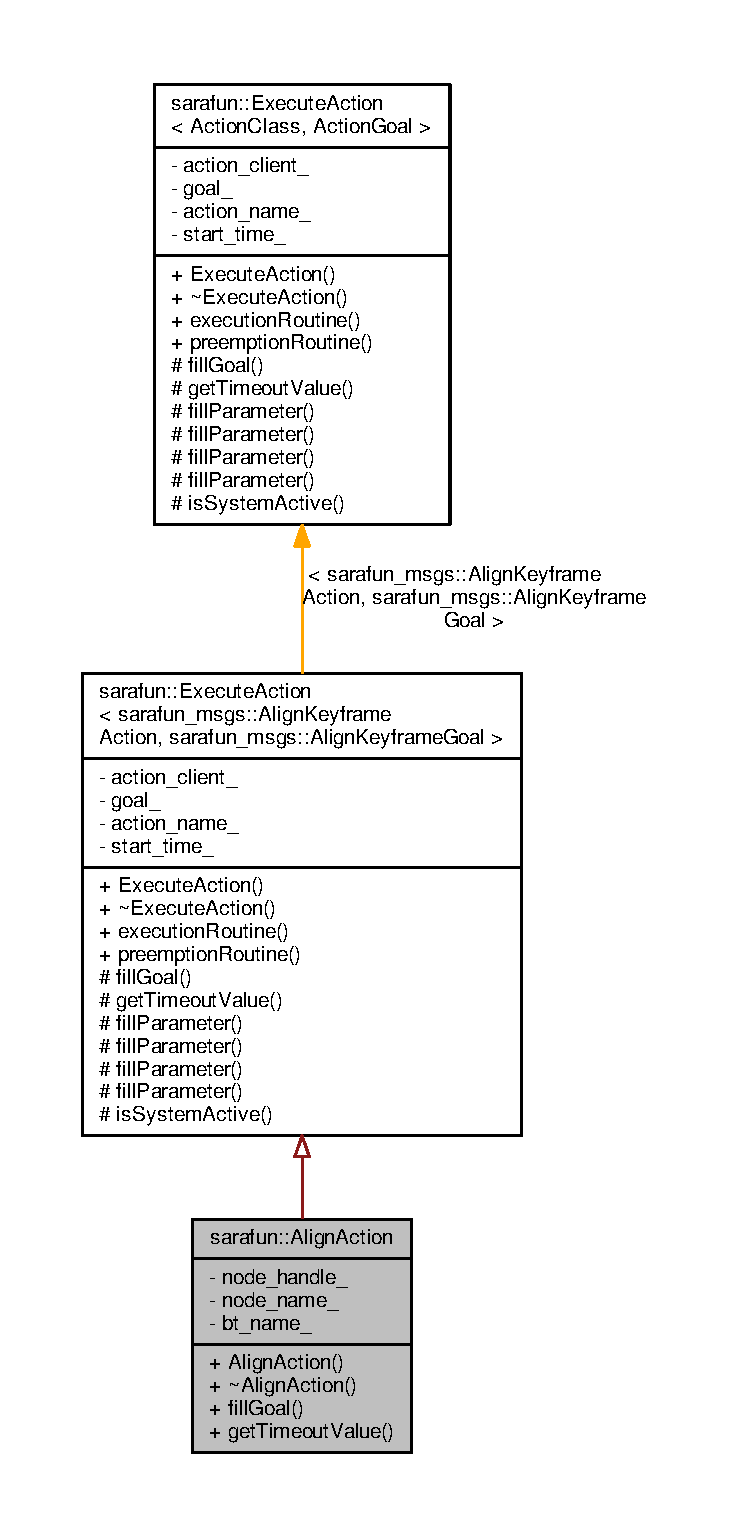
\includegraphics[height=550pt]{dc/d01/classsarafun_1_1AlignAction__inherit__graph}
\end{center}
\end{figure}


Collaboration diagram for sarafun\-:\-:Align\-Action\-:
\nopagebreak
\begin{figure}[H]
\begin{center}
\leavevmode
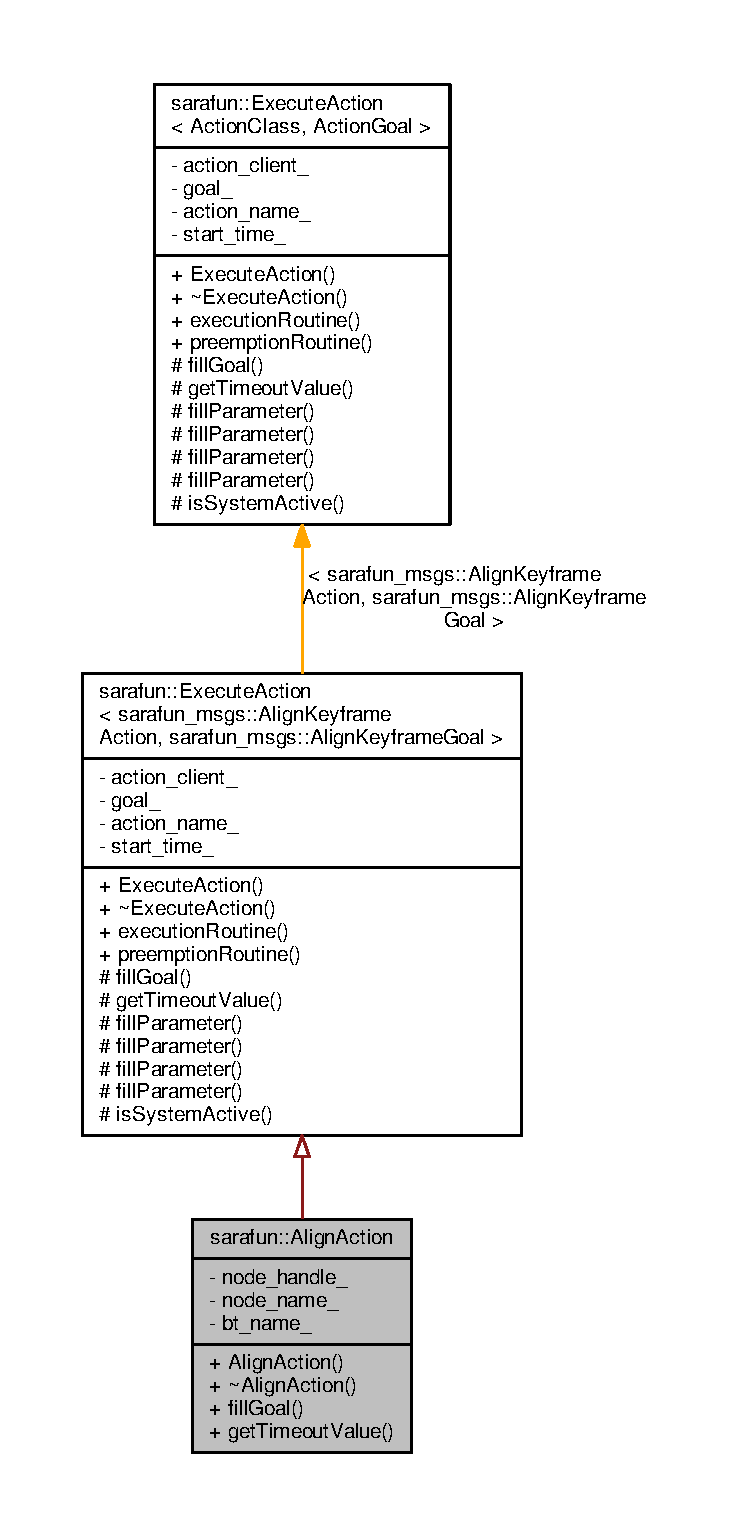
\includegraphics[height=550pt]{d2/d13/classsarafun_1_1AlignAction__coll__graph}
\end{center}
\end{figure}
\subsection*{Public Member Functions}
\begin{DoxyCompactItemize}
\item 
\hyperlink{classsarafun_1_1AlignAction_a013ed290585167a2693728565a764205_a013ed290585167a2693728565a764205}{Align\-Action} (std\-::string node\-\_\-name, std\-::string action\-\_\-name, std\-::string bt\-\_\-name)
\item 
\hyperlink{classsarafun_1_1AlignAction_a0fdb2f1de94801608024fb7dddd84f57_a0fdb2f1de94801608024fb7dddd84f57}{$\sim$\-Align\-Action} ()
\item 
bool \hyperlink{classsarafun_1_1AlignAction_ab92a62085ebd60438638b7b6c56da786_ab92a62085ebd60438638b7b6c56da786}{fill\-Goal} (sarafun\-\_\-msgs\-::\-Align\-Keyframe\-Goal \&goal)
\item 
double \hyperlink{classsarafun_1_1AlignAction_a9b9741ec3203bdc1b2e7b7cecc96e6ed_a9b9741ec3203bdc1b2e7b7cecc96e6ed}{get\-Timeout\-Value} ()
\end{DoxyCompactItemize}
\subsection*{Private Attributes}
\begin{DoxyCompactItemize}
\item 
ros\-::\-Node\-Handle \hyperlink{classsarafun_1_1AlignAction_acd1525d3ad1ad220e91af0c58802b6cf_acd1525d3ad1ad220e91af0c58802b6cf}{node\-\_\-handle\-\_\-}
\item 
std\-::string \hyperlink{classsarafun_1_1AlignAction_a4759b5ee1ef49d647eedcd8d04288799_a4759b5ee1ef49d647eedcd8d04288799}{node\-\_\-name\-\_\-}
\item 
std\-::string \hyperlink{classsarafun_1_1AlignAction_a832ecc3a169caf20ce7cb6f45d1551e3_a832ecc3a169caf20ce7cb6f45d1551e3}{bt\-\_\-name\-\_\-}
\end{DoxyCompactItemize}
\subsection*{Additional Inherited Members}


\subsection{Detailed Description}


Definition at line 9 of file Align\-Action.\-h.



\subsection{Constructor \& Destructor Documentation}
\hypertarget{classsarafun_1_1AlignAction_a013ed290585167a2693728565a764205_a013ed290585167a2693728565a764205}{\index{sarafun\-::\-Align\-Action@{sarafun\-::\-Align\-Action}!Align\-Action@{Align\-Action}}
\index{Align\-Action@{Align\-Action}!sarafun::AlignAction@{sarafun\-::\-Align\-Action}}
\subsubsection[{Align\-Action}]{\setlength{\rightskip}{0pt plus 5cm}sarafun\-::\-Align\-Action\-::\-Align\-Action (
\begin{DoxyParamCaption}
\item[{std\-::string}]{node\-\_\-name, }
\item[{std\-::string}]{action\-\_\-name, }
\item[{std\-::string}]{bt\-\_\-name}
\end{DoxyParamCaption}
)\hspace{0.3cm}{\ttfamily [inline]}}}\label{classsarafun_1_1AlignAction_a013ed290585167a2693728565a764205_a013ed290585167a2693728565a764205}


Definition at line 13 of file Align\-Action.\-h.



References node\-\_\-handle\-\_\-.

\hypertarget{classsarafun_1_1AlignAction_a0fdb2f1de94801608024fb7dddd84f57_a0fdb2f1de94801608024fb7dddd84f57}{\index{sarafun\-::\-Align\-Action@{sarafun\-::\-Align\-Action}!$\sim$\-Align\-Action@{$\sim$\-Align\-Action}}
\index{$\sim$\-Align\-Action@{$\sim$\-Align\-Action}!sarafun::AlignAction@{sarafun\-::\-Align\-Action}}
\subsubsection[{$\sim$\-Align\-Action}]{\setlength{\rightskip}{0pt plus 5cm}sarafun\-::\-Align\-Action\-::$\sim$\-Align\-Action (
\begin{DoxyParamCaption}
{}
\end{DoxyParamCaption}
)\hspace{0.3cm}{\ttfamily [inline]}}}\label{classsarafun_1_1AlignAction_a0fdb2f1de94801608024fb7dddd84f57_a0fdb2f1de94801608024fb7dddd84f57}


Definition at line 23 of file Align\-Action.\-h.



\subsection{Member Function Documentation}
\hypertarget{classsarafun_1_1AlignAction_ab92a62085ebd60438638b7b6c56da786_ab92a62085ebd60438638b7b6c56da786}{\index{sarafun\-::\-Align\-Action@{sarafun\-::\-Align\-Action}!fill\-Goal@{fill\-Goal}}
\index{fill\-Goal@{fill\-Goal}!sarafun::AlignAction@{sarafun\-::\-Align\-Action}}
\subsubsection[{fill\-Goal}]{\setlength{\rightskip}{0pt plus 5cm}bool sarafun\-::\-Align\-Action\-::fill\-Goal (
\begin{DoxyParamCaption}
\item[{sarafun\-\_\-msgs\-::\-Align\-Keyframe\-Goal \&}]{goal}
\end{DoxyParamCaption}
)\hspace{0.3cm}{\ttfamily [virtual]}}}\label{classsarafun_1_1AlignAction_ab92a62085ebd60438638b7b6c56da786_ab92a62085ebd60438638b7b6c56da786}
Fills in the goal for a particular action.


\begin{DoxyParams}{Parameters}
{\em goal} & The actionlib goal message of the externally implemented action. \\
\hline
\end{DoxyParams}
\begin{DoxyReturn}{Returns}
False in case of error, true otherwise. 
\end{DoxyReturn}


Implements \hyperlink{classsarafun_1_1ExecuteAction_a6dd9c0f013d15a17d7e7ce8dbe40a436_a6dd9c0f013d15a17d7e7ce8dbe40a436}{sarafun\-::\-Execute\-Action$<$ sarafun\-\_\-msgs\-::\-Align\-Keyframe\-Action, sarafun\-\_\-msgs\-::\-Align\-Keyframe\-Goal $>$}.



Definition at line 4 of file Align\-Action.\-cpp.



References sarafun\-::\-Execute\-Action$<$ sarafun\-\_\-msgs\-::\-Align\-Keyframe\-Action, sarafun\-\_\-msgs\-::\-Align\-Keyframe\-Goal $>$\-::fill\-Parameter().



Here is the call graph for this function\-:
\nopagebreak
\begin{figure}[H]
\begin{center}
\leavevmode
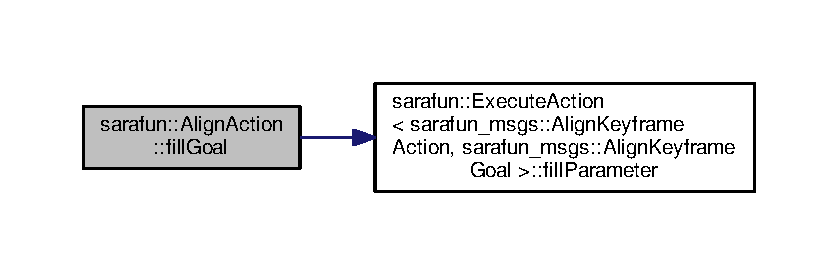
\includegraphics[width=350pt]{dc/df5/classsarafun_1_1AlignAction_ab92a62085ebd60438638b7b6c56da786_ab92a62085ebd60438638b7b6c56da786_cgraph}
\end{center}
\end{figure}


\hypertarget{classsarafun_1_1AlignAction_a9b9741ec3203bdc1b2e7b7cecc96e6ed_a9b9741ec3203bdc1b2e7b7cecc96e6ed}{\index{sarafun\-::\-Align\-Action@{sarafun\-::\-Align\-Action}!get\-Timeout\-Value@{get\-Timeout\-Value}}
\index{get\-Timeout\-Value@{get\-Timeout\-Value}!sarafun::AlignAction@{sarafun\-::\-Align\-Action}}
\subsubsection[{get\-Timeout\-Value}]{\setlength{\rightskip}{0pt plus 5cm}double sarafun\-::\-Align\-Action\-::get\-Timeout\-Value (
\begin{DoxyParamCaption}
{}
\end{DoxyParamCaption}
)\hspace{0.3cm}{\ttfamily [virtual]}}}\label{classsarafun_1_1AlignAction_a9b9741ec3203bdc1b2e7b7cecc96e6ed_a9b9741ec3203bdc1b2e7b7cecc96e6ed}
Provides the client with a timeout value for actionlib connections.

\begin{DoxyReturn}{Returns}
The timeout value (in seconds). 
\end{DoxyReturn}


Implements \hyperlink{classsarafun_1_1ExecuteAction_aba6cfa8a8ce19e735eb6394424df6d17_aba6cfa8a8ce19e735eb6394424df6d17}{sarafun\-::\-Execute\-Action$<$ sarafun\-\_\-msgs\-::\-Align\-Keyframe\-Action, sarafun\-\_\-msgs\-::\-Align\-Keyframe\-Goal $>$}.



Definition at line 13 of file Align\-Action.\-cpp.



References sarafun\-::\-Execute\-Action$<$ sarafun\-\_\-msgs\-::\-Align\-Keyframe\-Action, sarafun\-\_\-msgs\-::\-Align\-Keyframe\-Goal $>$\-::fill\-Parameter().



Here is the call graph for this function\-:
\nopagebreak
\begin{figure}[H]
\begin{center}
\leavevmode
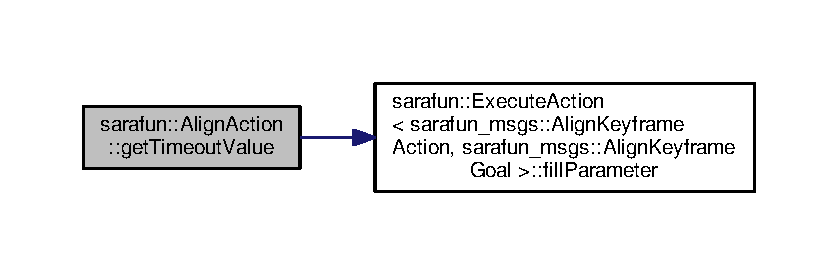
\includegraphics[width=350pt]{dc/df5/classsarafun_1_1AlignAction_a9b9741ec3203bdc1b2e7b7cecc96e6ed_a9b9741ec3203bdc1b2e7b7cecc96e6ed_cgraph}
\end{center}
\end{figure}




\subsection{Field Documentation}
\hypertarget{classsarafun_1_1AlignAction_a832ecc3a169caf20ce7cb6f45d1551e3_a832ecc3a169caf20ce7cb6f45d1551e3}{\index{sarafun\-::\-Align\-Action@{sarafun\-::\-Align\-Action}!bt\-\_\-name\-\_\-@{bt\-\_\-name\-\_\-}}
\index{bt\-\_\-name\-\_\-@{bt\-\_\-name\-\_\-}!sarafun::AlignAction@{sarafun\-::\-Align\-Action}}
\subsubsection[{bt\-\_\-name\-\_\-}]{\setlength{\rightskip}{0pt plus 5cm}std\-::string sarafun\-::\-Align\-Action\-::bt\-\_\-name\-\_\-\hspace{0.3cm}{\ttfamily [private]}}}\label{classsarafun_1_1AlignAction_a832ecc3a169caf20ce7cb6f45d1551e3_a832ecc3a169caf20ce7cb6f45d1551e3}


Definition at line 31 of file Align\-Action.\-h.

\hypertarget{classsarafun_1_1AlignAction_acd1525d3ad1ad220e91af0c58802b6cf_acd1525d3ad1ad220e91af0c58802b6cf}{\index{sarafun\-::\-Align\-Action@{sarafun\-::\-Align\-Action}!node\-\_\-handle\-\_\-@{node\-\_\-handle\-\_\-}}
\index{node\-\_\-handle\-\_\-@{node\-\_\-handle\-\_\-}!sarafun::AlignAction@{sarafun\-::\-Align\-Action}}
\subsubsection[{node\-\_\-handle\-\_\-}]{\setlength{\rightskip}{0pt plus 5cm}ros\-::\-Node\-Handle sarafun\-::\-Align\-Action\-::node\-\_\-handle\-\_\-\hspace{0.3cm}{\ttfamily [private]}}}\label{classsarafun_1_1AlignAction_acd1525d3ad1ad220e91af0c58802b6cf_acd1525d3ad1ad220e91af0c58802b6cf}


Definition at line 29 of file Align\-Action.\-h.



Referenced by Align\-Action().

\hypertarget{classsarafun_1_1AlignAction_a4759b5ee1ef49d647eedcd8d04288799_a4759b5ee1ef49d647eedcd8d04288799}{\index{sarafun\-::\-Align\-Action@{sarafun\-::\-Align\-Action}!node\-\_\-name\-\_\-@{node\-\_\-name\-\_\-}}
\index{node\-\_\-name\-\_\-@{node\-\_\-name\-\_\-}!sarafun::AlignAction@{sarafun\-::\-Align\-Action}}
\subsubsection[{node\-\_\-name\-\_\-}]{\setlength{\rightskip}{0pt plus 5cm}std\-::string sarafun\-::\-Align\-Action\-::node\-\_\-name\-\_\-\hspace{0.3cm}{\ttfamily [private]}}}\label{classsarafun_1_1AlignAction_a4759b5ee1ef49d647eedcd8d04288799_a4759b5ee1ef49d647eedcd8d04288799}


Definition at line 30 of file Align\-Action.\-h.



The documentation for this class was generated from the following files\-:\begin{DoxyCompactItemize}
\item 
Align\-Action.\-h\item 
Align\-Action.\-cpp\end{DoxyCompactItemize}

\hypertarget{classsarafun_1_1ApproachObjectsAction}{\section{sarafun\-:\-:Approach\-Objects\-Action Class Reference}
\label{classsarafun_1_1ApproachObjectsAction}\index{sarafun\-::\-Approach\-Objects\-Action@{sarafun\-::\-Approach\-Objects\-Action}}
}


{\ttfamily \#include $<$Approach\-Objects\-Action.\-h$>$}

Inheritance diagram for sarafun\-:\-:Approach\-Objects\-Action\-:\begin{figure}[H]
\begin{center}
\leavevmode
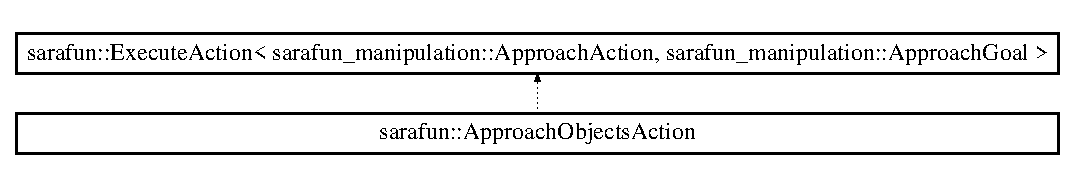
\includegraphics[height=1.839080cm]{classsarafun_1_1ApproachObjectsAction}
\end{center}
\end{figure}
\subsection*{Public Member Functions}
\begin{DoxyCompactItemize}
\item 
\hyperlink{classsarafun_1_1ApproachObjectsAction_ab0d857c262d75eeb85d8dc0e8f746f5f}{Approach\-Objects\-Action} (std\-::string node\-\_\-name, std\-::string action\-\_\-name, std\-::string bt\-\_\-name)
\item 
\hyperlink{classsarafun_1_1ApproachObjectsAction_adb6adaf7dae2e4addf53f47f07afd21e}{$\sim$\-Approach\-Objects\-Action} ()
\item 
bool \hyperlink{classsarafun_1_1ApproachObjectsAction_af5d216551122da780bc550daf4f1dca4}{fill\-Goal} (sarafun\-\_\-manipulation\-::\-Approach\-Goal \&goal)
\item 
double \hyperlink{classsarafun_1_1ApproachObjectsAction_a6852994a6e8a1edf9b2c24c91fd07df2}{get\-Timeout\-Value} ()
\end{DoxyCompactItemize}


\subsection{Constructor \& Destructor Documentation}
\hypertarget{classsarafun_1_1ApproachObjectsAction_ab0d857c262d75eeb85d8dc0e8f746f5f}{\index{sarafun\-::\-Approach\-Objects\-Action@{sarafun\-::\-Approach\-Objects\-Action}!Approach\-Objects\-Action@{Approach\-Objects\-Action}}
\index{Approach\-Objects\-Action@{Approach\-Objects\-Action}!sarafun::ApproachObjectsAction@{sarafun\-::\-Approach\-Objects\-Action}}
\subsubsection[{Approach\-Objects\-Action}]{\setlength{\rightskip}{0pt plus 5cm}sarafun\-::\-Approach\-Objects\-Action\-::\-Approach\-Objects\-Action (
\begin{DoxyParamCaption}
\item[{std\-::string}]{node\-\_\-name, }
\item[{std\-::string}]{action\-\_\-name, }
\item[{std\-::string}]{bt\-\_\-name}
\end{DoxyParamCaption}
)\hspace{0.3cm}{\ttfamily [inline]}}}\label{classsarafun_1_1ApproachObjectsAction_ab0d857c262d75eeb85d8dc0e8f746f5f}
\hypertarget{classsarafun_1_1ApproachObjectsAction_adb6adaf7dae2e4addf53f47f07afd21e}{\index{sarafun\-::\-Approach\-Objects\-Action@{sarafun\-::\-Approach\-Objects\-Action}!$\sim$\-Approach\-Objects\-Action@{$\sim$\-Approach\-Objects\-Action}}
\index{$\sim$\-Approach\-Objects\-Action@{$\sim$\-Approach\-Objects\-Action}!sarafun::ApproachObjectsAction@{sarafun\-::\-Approach\-Objects\-Action}}
\subsubsection[{$\sim$\-Approach\-Objects\-Action}]{\setlength{\rightskip}{0pt plus 5cm}sarafun\-::\-Approach\-Objects\-Action\-::$\sim$\-Approach\-Objects\-Action (
\begin{DoxyParamCaption}
{}
\end{DoxyParamCaption}
)\hspace{0.3cm}{\ttfamily [inline]}}}\label{classsarafun_1_1ApproachObjectsAction_adb6adaf7dae2e4addf53f47f07afd21e}


\subsection{Member Function Documentation}
\hypertarget{classsarafun_1_1ApproachObjectsAction_af5d216551122da780bc550daf4f1dca4}{\index{sarafun\-::\-Approach\-Objects\-Action@{sarafun\-::\-Approach\-Objects\-Action}!fill\-Goal@{fill\-Goal}}
\index{fill\-Goal@{fill\-Goal}!sarafun::ApproachObjectsAction@{sarafun\-::\-Approach\-Objects\-Action}}
\subsubsection[{fill\-Goal}]{\setlength{\rightskip}{0pt plus 5cm}bool sarafun\-::\-Approach\-Objects\-Action\-::fill\-Goal (
\begin{DoxyParamCaption}
\item[{sarafun\-\_\-manipulation\-::\-Approach\-Goal \&}]{goal}
\end{DoxyParamCaption}
)\hspace{0.3cm}{\ttfamily [virtual]}}}\label{classsarafun_1_1ApproachObjectsAction_af5d216551122da780bc550daf4f1dca4}
Fills in the goal for a particular action.


\begin{DoxyParams}{Parameters}
{\em goal} & The actionlib goal message of the externally implemented action. \\
\hline
\end{DoxyParams}
\begin{DoxyReturn}{Returns}
False in case of error, true otherwise. 
\end{DoxyReturn}


Implements \hyperlink{classsarafun_1_1ExecuteAction_a6dd9c0f013d15a17d7e7ce8dbe40a436}{sarafun\-::\-Execute\-Action$<$ sarafun\-\_\-manipulation\-::\-Approach\-Action, sarafun\-\_\-manipulation\-::\-Approach\-Goal $>$}.

\hypertarget{classsarafun_1_1ApproachObjectsAction_a6852994a6e8a1edf9b2c24c91fd07df2}{\index{sarafun\-::\-Approach\-Objects\-Action@{sarafun\-::\-Approach\-Objects\-Action}!get\-Timeout\-Value@{get\-Timeout\-Value}}
\index{get\-Timeout\-Value@{get\-Timeout\-Value}!sarafun::ApproachObjectsAction@{sarafun\-::\-Approach\-Objects\-Action}}
\subsubsection[{get\-Timeout\-Value}]{\setlength{\rightskip}{0pt plus 5cm}double sarafun\-::\-Approach\-Objects\-Action\-::get\-Timeout\-Value (
\begin{DoxyParamCaption}
{}
\end{DoxyParamCaption}
)\hspace{0.3cm}{\ttfamily [virtual]}}}\label{classsarafun_1_1ApproachObjectsAction_a6852994a6e8a1edf9b2c24c91fd07df2}
Provides the client with a timeout value for actionlib connections.

\begin{DoxyReturn}{Returns}
The timeout value (in seconds). 
\end{DoxyReturn}


Implements \hyperlink{classsarafun_1_1ExecuteAction_aba6cfa8a8ce19e735eb6394424df6d17}{sarafun\-::\-Execute\-Action$<$ sarafun\-\_\-manipulation\-::\-Approach\-Action, sarafun\-\_\-manipulation\-::\-Approach\-Goal $>$}.



The documentation for this class was generated from the following files\-:\begin{DoxyCompactItemize}
\item 
sarafun\-\_\-tree/include/sarafun\-\_\-tree/demo\-\_\-bt\-\_\-nodes/\hyperlink{ApproachObjectsAction_8h}{Approach\-Objects\-Action.\-h}\item 
sarafun\-\_\-tree/src/demo\-\_\-bt\-\_\-nodes/\hyperlink{ApproachObjectsAction_8cpp}{Approach\-Objects\-Action.\-cpp}\end{DoxyCompactItemize}

\hypertarget{classsarafun_1_1AssembledAction}{\section{sarafun\-:\-:Assembled\-Action Class Reference}
\label{classsarafun_1_1AssembledAction}\index{sarafun\-::\-Assembled\-Action@{sarafun\-::\-Assembled\-Action}}
}


{\ttfamily \#include $<$Assembled\-Action.\-h$>$}



Inheritance diagram for sarafun\-:\-:Assembled\-Action\-:
\nopagebreak
\begin{figure}[H]
\begin{center}
\leavevmode
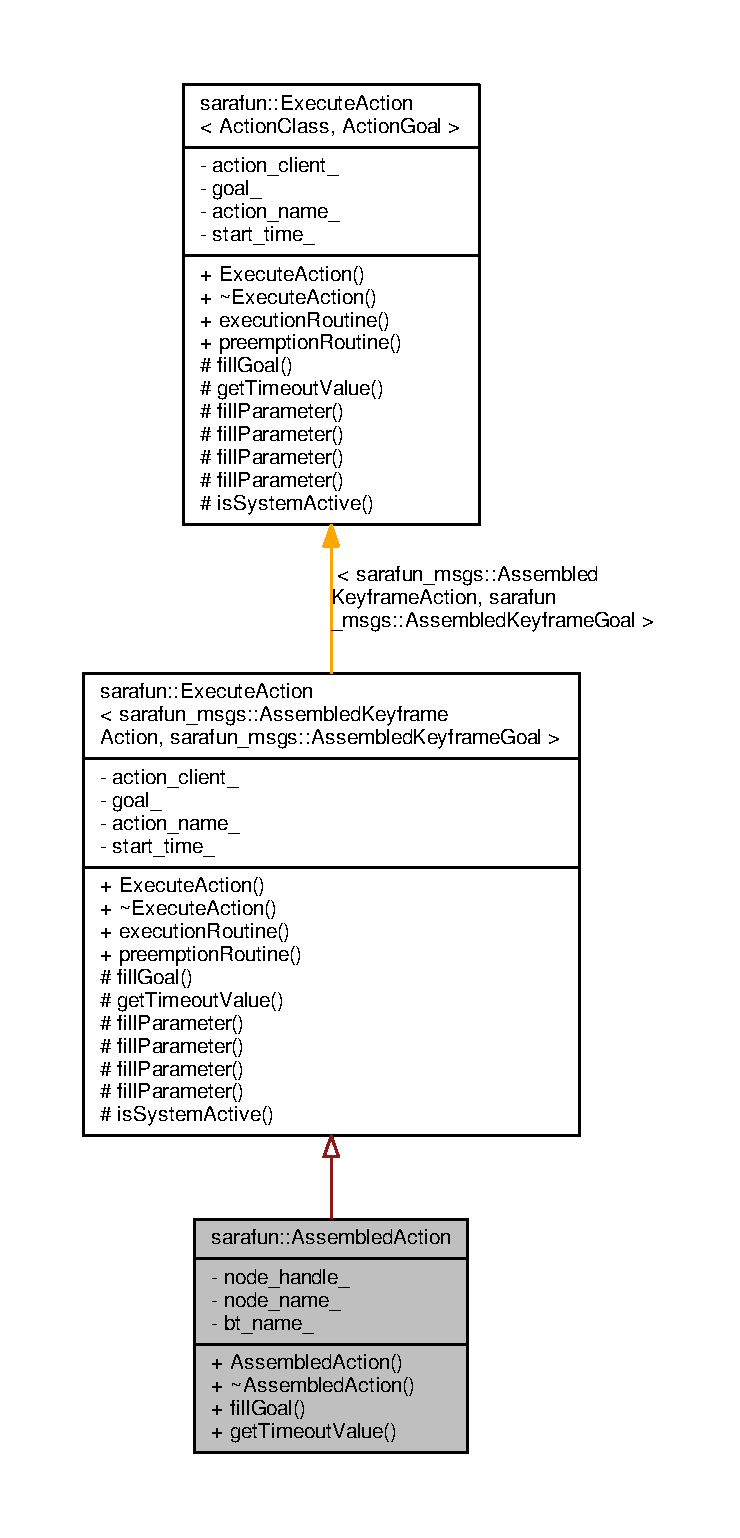
\includegraphics[height=550pt]{d9/d73/classsarafun_1_1AssembledAction__inherit__graph}
\end{center}
\end{figure}


Collaboration diagram for sarafun\-:\-:Assembled\-Action\-:
\nopagebreak
\begin{figure}[H]
\begin{center}
\leavevmode
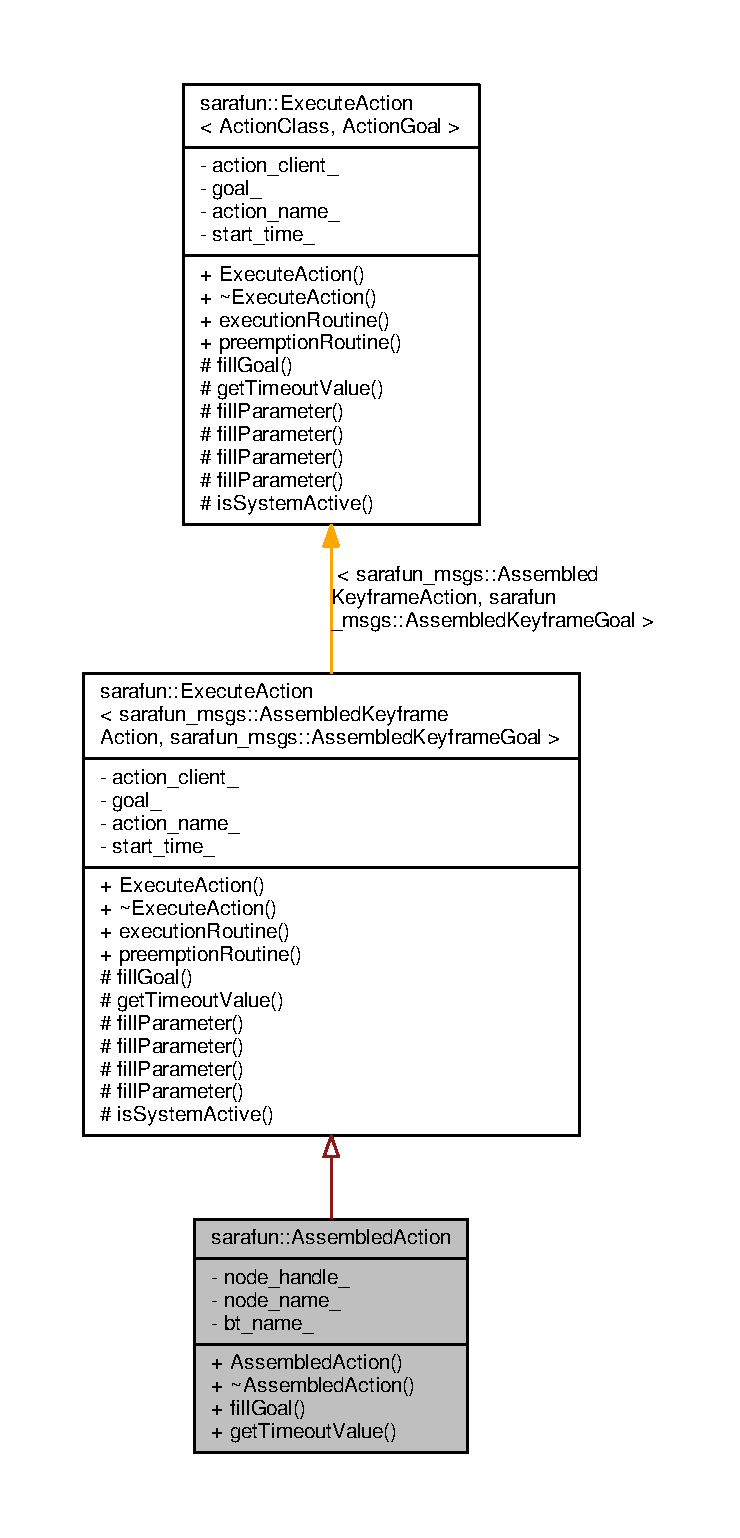
\includegraphics[height=550pt]{d7/df2/classsarafun_1_1AssembledAction__coll__graph}
\end{center}
\end{figure}
\subsection*{Public Member Functions}
\begin{DoxyCompactItemize}
\item 
\hyperlink{classsarafun_1_1AssembledAction_a0207a1b903e0189627087d7ed71bc130_a0207a1b903e0189627087d7ed71bc130}{Assembled\-Action} (std\-::string node\-\_\-name, std\-::string action\-\_\-name, std\-::string bt\-\_\-name)
\item 
\hyperlink{classsarafun_1_1AssembledAction_a8d290f1548b55bca1995df599272fc2f_a8d290f1548b55bca1995df599272fc2f}{$\sim$\-Assembled\-Action} ()
\item 
bool \hyperlink{classsarafun_1_1AssembledAction_a094a5cfde4d6bb6d024256834e771a39_a094a5cfde4d6bb6d024256834e771a39}{fill\-Goal} (sarafun\-\_\-msgs\-::\-Assembled\-Keyframe\-Goal \&goal)
\item 
double \hyperlink{classsarafun_1_1AssembledAction_ade9095a291dce652339238d137419b49_ade9095a291dce652339238d137419b49}{get\-Timeout\-Value} ()
\end{DoxyCompactItemize}
\subsection*{Private Attributes}
\begin{DoxyCompactItemize}
\item 
ros\-::\-Node\-Handle \hyperlink{classsarafun_1_1AssembledAction_ae97c585b30dd24e64cc08f78c08e52c5_ae97c585b30dd24e64cc08f78c08e52c5}{node\-\_\-handle\-\_\-}
\item 
std\-::string \hyperlink{classsarafun_1_1AssembledAction_a693b73bd880c4b9c193dea5ab62c1df8_a693b73bd880c4b9c193dea5ab62c1df8}{node\-\_\-name\-\_\-}
\item 
std\-::string \hyperlink{classsarafun_1_1AssembledAction_a4dae92c3c98d924c35f9cda69ede136d_a4dae92c3c98d924c35f9cda69ede136d}{bt\-\_\-name\-\_\-}
\end{DoxyCompactItemize}
\subsection*{Additional Inherited Members}


\subsection{Detailed Description}


Definition at line 9 of file Assembled\-Action.\-h.



\subsection{Constructor \& Destructor Documentation}
\hypertarget{classsarafun_1_1AssembledAction_a0207a1b903e0189627087d7ed71bc130_a0207a1b903e0189627087d7ed71bc130}{\index{sarafun\-::\-Assembled\-Action@{sarafun\-::\-Assembled\-Action}!Assembled\-Action@{Assembled\-Action}}
\index{Assembled\-Action@{Assembled\-Action}!sarafun::AssembledAction@{sarafun\-::\-Assembled\-Action}}
\subsubsection[{Assembled\-Action}]{\setlength{\rightskip}{0pt plus 5cm}sarafun\-::\-Assembled\-Action\-::\-Assembled\-Action (
\begin{DoxyParamCaption}
\item[{std\-::string}]{node\-\_\-name, }
\item[{std\-::string}]{action\-\_\-name, }
\item[{std\-::string}]{bt\-\_\-name}
\end{DoxyParamCaption}
)\hspace{0.3cm}{\ttfamily [inline]}}}\label{classsarafun_1_1AssembledAction_a0207a1b903e0189627087d7ed71bc130_a0207a1b903e0189627087d7ed71bc130}


Definition at line 13 of file Assembled\-Action.\-h.



References node\-\_\-handle\-\_\-.

\hypertarget{classsarafun_1_1AssembledAction_a8d290f1548b55bca1995df599272fc2f_a8d290f1548b55bca1995df599272fc2f}{\index{sarafun\-::\-Assembled\-Action@{sarafun\-::\-Assembled\-Action}!$\sim$\-Assembled\-Action@{$\sim$\-Assembled\-Action}}
\index{$\sim$\-Assembled\-Action@{$\sim$\-Assembled\-Action}!sarafun::AssembledAction@{sarafun\-::\-Assembled\-Action}}
\subsubsection[{$\sim$\-Assembled\-Action}]{\setlength{\rightskip}{0pt plus 5cm}sarafun\-::\-Assembled\-Action\-::$\sim$\-Assembled\-Action (
\begin{DoxyParamCaption}
{}
\end{DoxyParamCaption}
)\hspace{0.3cm}{\ttfamily [inline]}}}\label{classsarafun_1_1AssembledAction_a8d290f1548b55bca1995df599272fc2f_a8d290f1548b55bca1995df599272fc2f}


Definition at line 23 of file Assembled\-Action.\-h.



\subsection{Member Function Documentation}
\hypertarget{classsarafun_1_1AssembledAction_a094a5cfde4d6bb6d024256834e771a39_a094a5cfde4d6bb6d024256834e771a39}{\index{sarafun\-::\-Assembled\-Action@{sarafun\-::\-Assembled\-Action}!fill\-Goal@{fill\-Goal}}
\index{fill\-Goal@{fill\-Goal}!sarafun::AssembledAction@{sarafun\-::\-Assembled\-Action}}
\subsubsection[{fill\-Goal}]{\setlength{\rightskip}{0pt plus 5cm}bool sarafun\-::\-Assembled\-Action\-::fill\-Goal (
\begin{DoxyParamCaption}
\item[{sarafun\-\_\-msgs\-::\-Assembled\-Keyframe\-Goal \&}]{goal}
\end{DoxyParamCaption}
)\hspace{0.3cm}{\ttfamily [virtual]}}}\label{classsarafun_1_1AssembledAction_a094a5cfde4d6bb6d024256834e771a39_a094a5cfde4d6bb6d024256834e771a39}
Fills in the goal for a particular action.


\begin{DoxyParams}{Parameters}
{\em goal} & The actionlib goal message of the externally implemented action. \\
\hline
\end{DoxyParams}
\begin{DoxyReturn}{Returns}
False in case of error, true otherwise. 
\end{DoxyReturn}


Implements \hyperlink{classsarafun_1_1ExecuteAction_a6dd9c0f013d15a17d7e7ce8dbe40a436_a6dd9c0f013d15a17d7e7ce8dbe40a436}{sarafun\-::\-Execute\-Action$<$ sarafun\-\_\-msgs\-::\-Assembled\-Keyframe\-Action, sarafun\-\_\-msgs\-::\-Assembled\-Keyframe\-Goal $>$}.



Definition at line 4 of file Assembled\-Action.\-cpp.



References sarafun\-::\-Execute\-Action$<$ sarafun\-\_\-msgs\-::\-Assembled\-Keyframe\-Action, sarafun\-\_\-msgs\-::\-Assembled\-Keyframe\-Goal $>$\-::fill\-Parameter().



Here is the call graph for this function\-:
\nopagebreak
\begin{figure}[H]
\begin{center}
\leavevmode
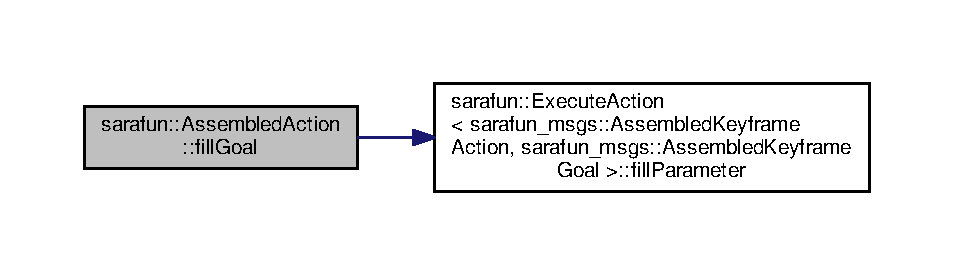
\includegraphics[width=350pt]{dc/d58/classsarafun_1_1AssembledAction_a094a5cfde4d6bb6d024256834e771a39_a094a5cfde4d6bb6d024256834e771a39_cgraph}
\end{center}
\end{figure}


\hypertarget{classsarafun_1_1AssembledAction_ade9095a291dce652339238d137419b49_ade9095a291dce652339238d137419b49}{\index{sarafun\-::\-Assembled\-Action@{sarafun\-::\-Assembled\-Action}!get\-Timeout\-Value@{get\-Timeout\-Value}}
\index{get\-Timeout\-Value@{get\-Timeout\-Value}!sarafun::AssembledAction@{sarafun\-::\-Assembled\-Action}}
\subsubsection[{get\-Timeout\-Value}]{\setlength{\rightskip}{0pt plus 5cm}double sarafun\-::\-Assembled\-Action\-::get\-Timeout\-Value (
\begin{DoxyParamCaption}
{}
\end{DoxyParamCaption}
)\hspace{0.3cm}{\ttfamily [virtual]}}}\label{classsarafun_1_1AssembledAction_ade9095a291dce652339238d137419b49_ade9095a291dce652339238d137419b49}
Provides the client with a timeout value for actionlib connections.

\begin{DoxyReturn}{Returns}
The timeout value (in seconds). 
\end{DoxyReturn}


Implements \hyperlink{classsarafun_1_1ExecuteAction_aba6cfa8a8ce19e735eb6394424df6d17_aba6cfa8a8ce19e735eb6394424df6d17}{sarafun\-::\-Execute\-Action$<$ sarafun\-\_\-msgs\-::\-Assembled\-Keyframe\-Action, sarafun\-\_\-msgs\-::\-Assembled\-Keyframe\-Goal $>$}.



Definition at line 13 of file Assembled\-Action.\-cpp.



References sarafun\-::\-Execute\-Action$<$ sarafun\-\_\-msgs\-::\-Assembled\-Keyframe\-Action, sarafun\-\_\-msgs\-::\-Assembled\-Keyframe\-Goal $>$\-::fill\-Parameter().



Here is the call graph for this function\-:
\nopagebreak
\begin{figure}[H]
\begin{center}
\leavevmode
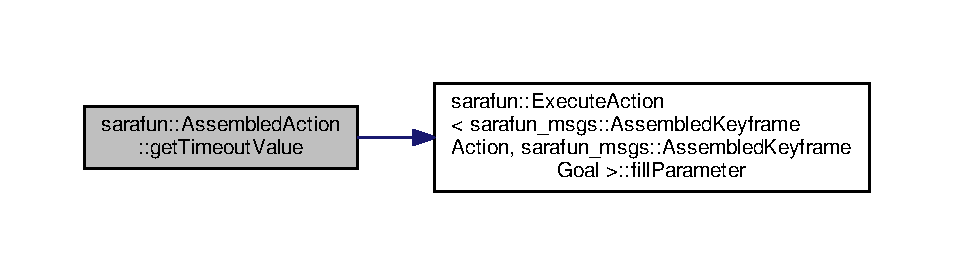
\includegraphics[width=350pt]{dc/d58/classsarafun_1_1AssembledAction_ade9095a291dce652339238d137419b49_ade9095a291dce652339238d137419b49_cgraph}
\end{center}
\end{figure}




\subsection{Field Documentation}
\hypertarget{classsarafun_1_1AssembledAction_a4dae92c3c98d924c35f9cda69ede136d_a4dae92c3c98d924c35f9cda69ede136d}{\index{sarafun\-::\-Assembled\-Action@{sarafun\-::\-Assembled\-Action}!bt\-\_\-name\-\_\-@{bt\-\_\-name\-\_\-}}
\index{bt\-\_\-name\-\_\-@{bt\-\_\-name\-\_\-}!sarafun::AssembledAction@{sarafun\-::\-Assembled\-Action}}
\subsubsection[{bt\-\_\-name\-\_\-}]{\setlength{\rightskip}{0pt plus 5cm}std\-::string sarafun\-::\-Assembled\-Action\-::bt\-\_\-name\-\_\-\hspace{0.3cm}{\ttfamily [private]}}}\label{classsarafun_1_1AssembledAction_a4dae92c3c98d924c35f9cda69ede136d_a4dae92c3c98d924c35f9cda69ede136d}


Definition at line 31 of file Assembled\-Action.\-h.

\hypertarget{classsarafun_1_1AssembledAction_ae97c585b30dd24e64cc08f78c08e52c5_ae97c585b30dd24e64cc08f78c08e52c5}{\index{sarafun\-::\-Assembled\-Action@{sarafun\-::\-Assembled\-Action}!node\-\_\-handle\-\_\-@{node\-\_\-handle\-\_\-}}
\index{node\-\_\-handle\-\_\-@{node\-\_\-handle\-\_\-}!sarafun::AssembledAction@{sarafun\-::\-Assembled\-Action}}
\subsubsection[{node\-\_\-handle\-\_\-}]{\setlength{\rightskip}{0pt plus 5cm}ros\-::\-Node\-Handle sarafun\-::\-Assembled\-Action\-::node\-\_\-handle\-\_\-\hspace{0.3cm}{\ttfamily [private]}}}\label{classsarafun_1_1AssembledAction_ae97c585b30dd24e64cc08f78c08e52c5_ae97c585b30dd24e64cc08f78c08e52c5}


Definition at line 29 of file Assembled\-Action.\-h.



Referenced by Assembled\-Action().

\hypertarget{classsarafun_1_1AssembledAction_a693b73bd880c4b9c193dea5ab62c1df8_a693b73bd880c4b9c193dea5ab62c1df8}{\index{sarafun\-::\-Assembled\-Action@{sarafun\-::\-Assembled\-Action}!node\-\_\-name\-\_\-@{node\-\_\-name\-\_\-}}
\index{node\-\_\-name\-\_\-@{node\-\_\-name\-\_\-}!sarafun::AssembledAction@{sarafun\-::\-Assembled\-Action}}
\subsubsection[{node\-\_\-name\-\_\-}]{\setlength{\rightskip}{0pt plus 5cm}std\-::string sarafun\-::\-Assembled\-Action\-::node\-\_\-name\-\_\-\hspace{0.3cm}{\ttfamily [private]}}}\label{classsarafun_1_1AssembledAction_a693b73bd880c4b9c193dea5ab62c1df8_a693b73bd880c4b9c193dea5ab62c1df8}


Definition at line 30 of file Assembled\-Action.\-h.



The documentation for this class was generated from the following files\-:\begin{DoxyCompactItemize}
\item 
Assembled\-Action.\-h\item 
Assembled\-Action.\-cpp\end{DoxyCompactItemize}

\hypertarget{classsarafun_1_1ContactAction}{\section{sarafun\-:\-:Contact\-Action Class Reference}
\label{classsarafun_1_1ContactAction}\index{sarafun\-::\-Contact\-Action@{sarafun\-::\-Contact\-Action}}
}


{\ttfamily \#include $<$Contact\-Action.\-h$>$}



Inheritance diagram for sarafun\-:\-:Contact\-Action\-:
\nopagebreak
\begin{figure}[H]
\begin{center}
\leavevmode
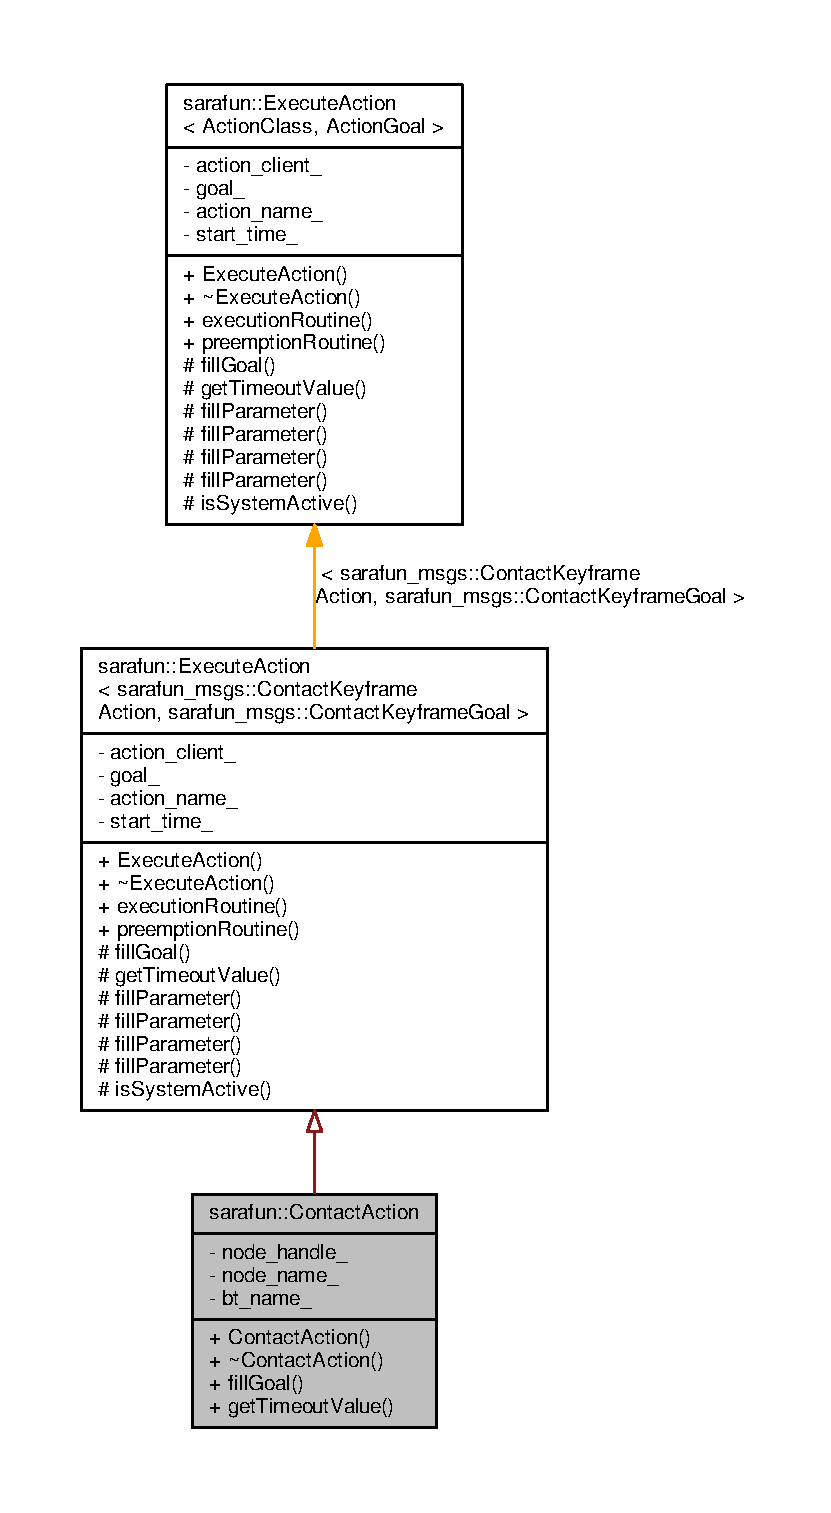
\includegraphics[height=550pt]{d8/d33/classsarafun_1_1ContactAction__inherit__graph}
\end{center}
\end{figure}


Collaboration diagram for sarafun\-:\-:Contact\-Action\-:
\nopagebreak
\begin{figure}[H]
\begin{center}
\leavevmode
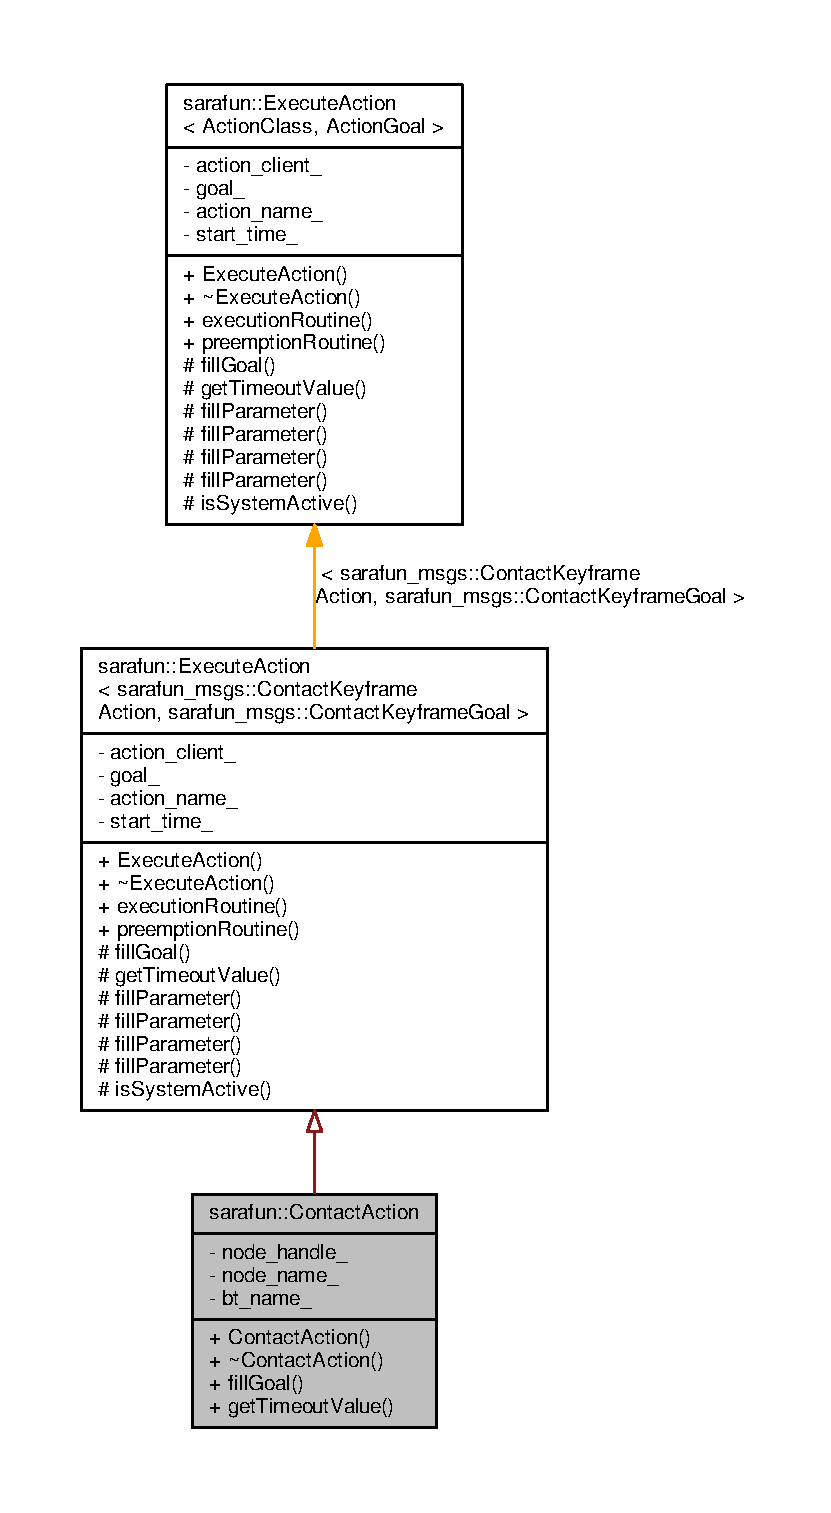
\includegraphics[height=550pt]{d3/d7e/classsarafun_1_1ContactAction__coll__graph}
\end{center}
\end{figure}
\subsection*{Public Member Functions}
\begin{DoxyCompactItemize}
\item 
\hyperlink{classsarafun_1_1ContactAction_a8374da0d20d05fe01b86f2090b2c1770_a8374da0d20d05fe01b86f2090b2c1770}{Contact\-Action} (std\-::string node\-\_\-name, std\-::string action\-\_\-name, std\-::string bt\-\_\-name)
\item 
\hyperlink{classsarafun_1_1ContactAction_a22429fcb44fbe815f745b4924ed08f34_a22429fcb44fbe815f745b4924ed08f34}{$\sim$\-Contact\-Action} ()
\item 
bool \hyperlink{classsarafun_1_1ContactAction_a563907411debe223088ef5a34d8c0fb0_a563907411debe223088ef5a34d8c0fb0}{fill\-Goal} (sarafun\-\_\-msgs\-::\-Contact\-Keyframe\-Goal \&goal)
\item 
double \hyperlink{classsarafun_1_1ContactAction_a85d81232d228fc6d2856d318d25c1bf9_a85d81232d228fc6d2856d318d25c1bf9}{get\-Timeout\-Value} ()
\end{DoxyCompactItemize}
\subsection*{Private Attributes}
\begin{DoxyCompactItemize}
\item 
ros\-::\-Node\-Handle \hyperlink{classsarafun_1_1ContactAction_a01f3f5f489242e0ec4add31d46fb8211_a01f3f5f489242e0ec4add31d46fb8211}{node\-\_\-handle\-\_\-}
\item 
std\-::string \hyperlink{classsarafun_1_1ContactAction_a1b1869bbc4525644b0986a0fbade1039_a1b1869bbc4525644b0986a0fbade1039}{node\-\_\-name\-\_\-}
\item 
std\-::string \hyperlink{classsarafun_1_1ContactAction_a71e5d4dc7682ec4dc8ca0b9b83ee214f_a71e5d4dc7682ec4dc8ca0b9b83ee214f}{bt\-\_\-name\-\_\-}
\end{DoxyCompactItemize}
\subsection*{Additional Inherited Members}


\subsection{Detailed Description}


Definition at line 9 of file Contact\-Action.\-h.



\subsection{Constructor \& Destructor Documentation}
\hypertarget{classsarafun_1_1ContactAction_a8374da0d20d05fe01b86f2090b2c1770_a8374da0d20d05fe01b86f2090b2c1770}{\index{sarafun\-::\-Contact\-Action@{sarafun\-::\-Contact\-Action}!Contact\-Action@{Contact\-Action}}
\index{Contact\-Action@{Contact\-Action}!sarafun::ContactAction@{sarafun\-::\-Contact\-Action}}
\subsubsection[{Contact\-Action}]{\setlength{\rightskip}{0pt plus 5cm}sarafun\-::\-Contact\-Action\-::\-Contact\-Action (
\begin{DoxyParamCaption}
\item[{std\-::string}]{node\-\_\-name, }
\item[{std\-::string}]{action\-\_\-name, }
\item[{std\-::string}]{bt\-\_\-name}
\end{DoxyParamCaption}
)\hspace{0.3cm}{\ttfamily [inline]}}}\label{classsarafun_1_1ContactAction_a8374da0d20d05fe01b86f2090b2c1770_a8374da0d20d05fe01b86f2090b2c1770}


Definition at line 13 of file Contact\-Action.\-h.



References node\-\_\-handle\-\_\-.

\hypertarget{classsarafun_1_1ContactAction_a22429fcb44fbe815f745b4924ed08f34_a22429fcb44fbe815f745b4924ed08f34}{\index{sarafun\-::\-Contact\-Action@{sarafun\-::\-Contact\-Action}!$\sim$\-Contact\-Action@{$\sim$\-Contact\-Action}}
\index{$\sim$\-Contact\-Action@{$\sim$\-Contact\-Action}!sarafun::ContactAction@{sarafun\-::\-Contact\-Action}}
\subsubsection[{$\sim$\-Contact\-Action}]{\setlength{\rightskip}{0pt plus 5cm}sarafun\-::\-Contact\-Action\-::$\sim$\-Contact\-Action (
\begin{DoxyParamCaption}
{}
\end{DoxyParamCaption}
)\hspace{0.3cm}{\ttfamily [inline]}}}\label{classsarafun_1_1ContactAction_a22429fcb44fbe815f745b4924ed08f34_a22429fcb44fbe815f745b4924ed08f34}


Definition at line 23 of file Contact\-Action.\-h.



\subsection{Member Function Documentation}
\hypertarget{classsarafun_1_1ContactAction_a563907411debe223088ef5a34d8c0fb0_a563907411debe223088ef5a34d8c0fb0}{\index{sarafun\-::\-Contact\-Action@{sarafun\-::\-Contact\-Action}!fill\-Goal@{fill\-Goal}}
\index{fill\-Goal@{fill\-Goal}!sarafun::ContactAction@{sarafun\-::\-Contact\-Action}}
\subsubsection[{fill\-Goal}]{\setlength{\rightskip}{0pt plus 5cm}bool sarafun\-::\-Contact\-Action\-::fill\-Goal (
\begin{DoxyParamCaption}
\item[{sarafun\-\_\-msgs\-::\-Contact\-Keyframe\-Goal \&}]{goal}
\end{DoxyParamCaption}
)\hspace{0.3cm}{\ttfamily [virtual]}}}\label{classsarafun_1_1ContactAction_a563907411debe223088ef5a34d8c0fb0_a563907411debe223088ef5a34d8c0fb0}
Fills in the goal for a particular action.


\begin{DoxyParams}{Parameters}
{\em goal} & The actionlib goal message of the externally implemented action. \\
\hline
\end{DoxyParams}
\begin{DoxyReturn}{Returns}
False in case of error, true otherwise. 
\end{DoxyReturn}


Implements \hyperlink{classsarafun_1_1ExecuteAction_a6dd9c0f013d15a17d7e7ce8dbe40a436_a6dd9c0f013d15a17d7e7ce8dbe40a436}{sarafun\-::\-Execute\-Action$<$ sarafun\-\_\-msgs\-::\-Contact\-Keyframe\-Action, sarafun\-\_\-msgs\-::\-Contact\-Keyframe\-Goal $>$}.



Definition at line 4 of file Contact\-Action.\-cpp.



References sarafun\-::\-Execute\-Action$<$ sarafun\-\_\-msgs\-::\-Contact\-Keyframe\-Action, sarafun\-\_\-msgs\-::\-Contact\-Keyframe\-Goal $>$\-::fill\-Parameter().



Here is the call graph for this function\-:
\nopagebreak
\begin{figure}[H]
\begin{center}
\leavevmode
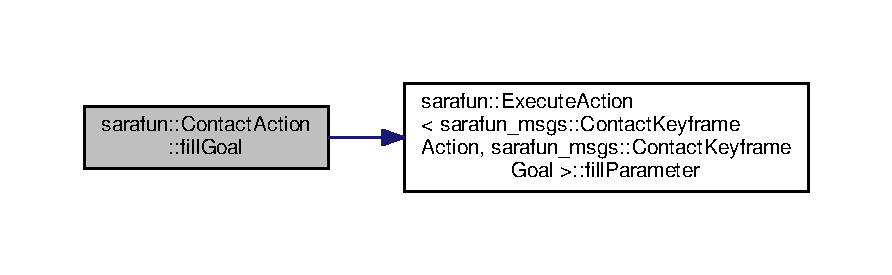
\includegraphics[width=350pt]{dc/d9f/classsarafun_1_1ContactAction_a563907411debe223088ef5a34d8c0fb0_a563907411debe223088ef5a34d8c0fb0_cgraph}
\end{center}
\end{figure}


\hypertarget{classsarafun_1_1ContactAction_a85d81232d228fc6d2856d318d25c1bf9_a85d81232d228fc6d2856d318d25c1bf9}{\index{sarafun\-::\-Contact\-Action@{sarafun\-::\-Contact\-Action}!get\-Timeout\-Value@{get\-Timeout\-Value}}
\index{get\-Timeout\-Value@{get\-Timeout\-Value}!sarafun::ContactAction@{sarafun\-::\-Contact\-Action}}
\subsubsection[{get\-Timeout\-Value}]{\setlength{\rightskip}{0pt plus 5cm}double sarafun\-::\-Contact\-Action\-::get\-Timeout\-Value (
\begin{DoxyParamCaption}
{}
\end{DoxyParamCaption}
)\hspace{0.3cm}{\ttfamily [virtual]}}}\label{classsarafun_1_1ContactAction_a85d81232d228fc6d2856d318d25c1bf9_a85d81232d228fc6d2856d318d25c1bf9}
Provides the client with a timeout value for actionlib connections.

\begin{DoxyReturn}{Returns}
The timeout value (in seconds). 
\end{DoxyReturn}


Implements \hyperlink{classsarafun_1_1ExecuteAction_aba6cfa8a8ce19e735eb6394424df6d17_aba6cfa8a8ce19e735eb6394424df6d17}{sarafun\-::\-Execute\-Action$<$ sarafun\-\_\-msgs\-::\-Contact\-Keyframe\-Action, sarafun\-\_\-msgs\-::\-Contact\-Keyframe\-Goal $>$}.



Definition at line 13 of file Contact\-Action.\-cpp.



References sarafun\-::\-Execute\-Action$<$ sarafun\-\_\-msgs\-::\-Contact\-Keyframe\-Action, sarafun\-\_\-msgs\-::\-Contact\-Keyframe\-Goal $>$\-::fill\-Parameter().



Here is the call graph for this function\-:
\nopagebreak
\begin{figure}[H]
\begin{center}
\leavevmode
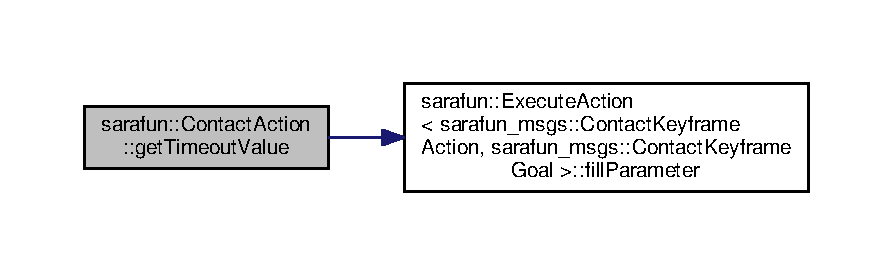
\includegraphics[width=350pt]{dc/d9f/classsarafun_1_1ContactAction_a85d81232d228fc6d2856d318d25c1bf9_a85d81232d228fc6d2856d318d25c1bf9_cgraph}
\end{center}
\end{figure}




\subsection{Field Documentation}
\hypertarget{classsarafun_1_1ContactAction_a71e5d4dc7682ec4dc8ca0b9b83ee214f_a71e5d4dc7682ec4dc8ca0b9b83ee214f}{\index{sarafun\-::\-Contact\-Action@{sarafun\-::\-Contact\-Action}!bt\-\_\-name\-\_\-@{bt\-\_\-name\-\_\-}}
\index{bt\-\_\-name\-\_\-@{bt\-\_\-name\-\_\-}!sarafun::ContactAction@{sarafun\-::\-Contact\-Action}}
\subsubsection[{bt\-\_\-name\-\_\-}]{\setlength{\rightskip}{0pt plus 5cm}std\-::string sarafun\-::\-Contact\-Action\-::bt\-\_\-name\-\_\-\hspace{0.3cm}{\ttfamily [private]}}}\label{classsarafun_1_1ContactAction_a71e5d4dc7682ec4dc8ca0b9b83ee214f_a71e5d4dc7682ec4dc8ca0b9b83ee214f}


Definition at line 31 of file Contact\-Action.\-h.

\hypertarget{classsarafun_1_1ContactAction_a01f3f5f489242e0ec4add31d46fb8211_a01f3f5f489242e0ec4add31d46fb8211}{\index{sarafun\-::\-Contact\-Action@{sarafun\-::\-Contact\-Action}!node\-\_\-handle\-\_\-@{node\-\_\-handle\-\_\-}}
\index{node\-\_\-handle\-\_\-@{node\-\_\-handle\-\_\-}!sarafun::ContactAction@{sarafun\-::\-Contact\-Action}}
\subsubsection[{node\-\_\-handle\-\_\-}]{\setlength{\rightskip}{0pt plus 5cm}ros\-::\-Node\-Handle sarafun\-::\-Contact\-Action\-::node\-\_\-handle\-\_\-\hspace{0.3cm}{\ttfamily [private]}}}\label{classsarafun_1_1ContactAction_a01f3f5f489242e0ec4add31d46fb8211_a01f3f5f489242e0ec4add31d46fb8211}


Definition at line 29 of file Contact\-Action.\-h.



Referenced by Contact\-Action().

\hypertarget{classsarafun_1_1ContactAction_a1b1869bbc4525644b0986a0fbade1039_a1b1869bbc4525644b0986a0fbade1039}{\index{sarafun\-::\-Contact\-Action@{sarafun\-::\-Contact\-Action}!node\-\_\-name\-\_\-@{node\-\_\-name\-\_\-}}
\index{node\-\_\-name\-\_\-@{node\-\_\-name\-\_\-}!sarafun::ContactAction@{sarafun\-::\-Contact\-Action}}
\subsubsection[{node\-\_\-name\-\_\-}]{\setlength{\rightskip}{0pt plus 5cm}std\-::string sarafun\-::\-Contact\-Action\-::node\-\_\-name\-\_\-\hspace{0.3cm}{\ttfamily [private]}}}\label{classsarafun_1_1ContactAction_a1b1869bbc4525644b0986a0fbade1039_a1b1869bbc4525644b0986a0fbade1039}


Definition at line 30 of file Contact\-Action.\-h.



The documentation for this class was generated from the following files\-:\begin{DoxyCompactItemize}
\item 
Contact\-Action.\-h\item 
Contact\-Action.\-cpp\end{DoxyCompactItemize}

\hypertarget{classsarafun_1_1ExecuteAction}{\section{sarafun\-:\-:Execute\-Action$<$ Action\-Class, Action\-Goal $>$ Class Template Reference}
\label{classsarafun_1_1ExecuteAction}\index{sarafun\-::\-Execute\-Action$<$ Action\-Class, Action\-Goal $>$@{sarafun\-::\-Execute\-Action$<$ Action\-Class, Action\-Goal $>$}}
}


{\ttfamily \#include $<$Execute\-Action.\-h$>$}



Inheritance diagram for sarafun\-:\-:Execute\-Action$<$ Action\-Class, Action\-Goal $>$\-:
\nopagebreak
\begin{figure}[H]
\begin{center}
\leavevmode
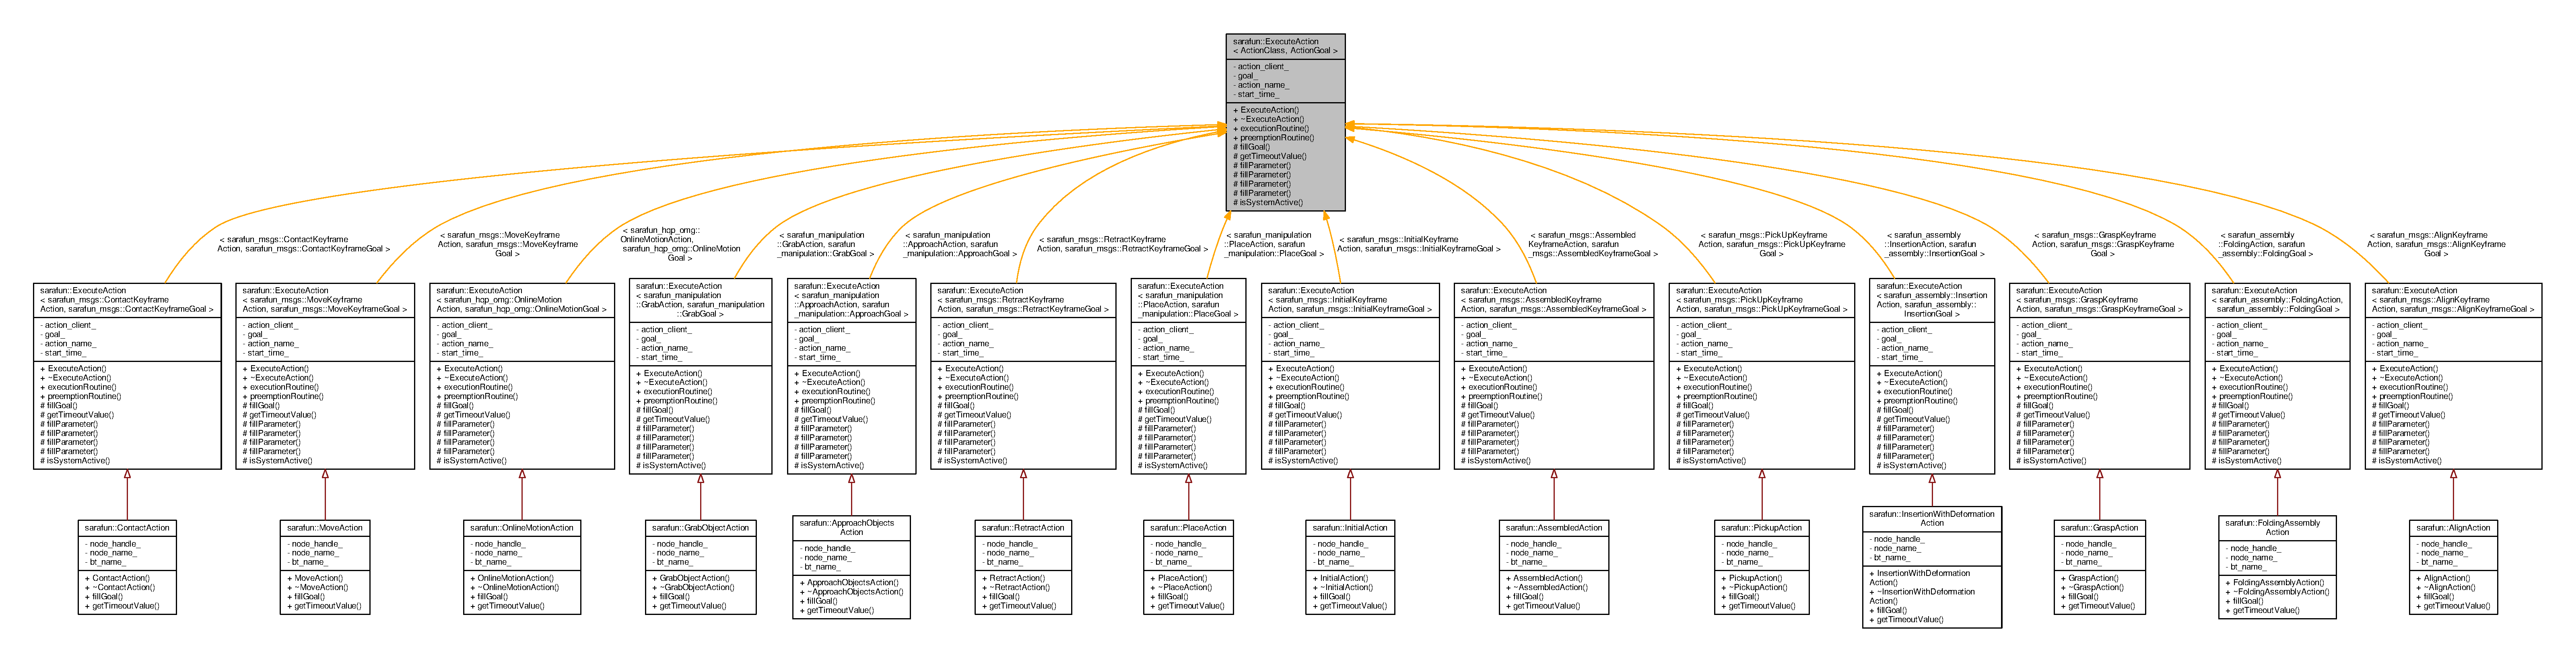
\includegraphics[width=350pt]{db/d30/classsarafun_1_1ExecuteAction__inherit__graph}
\end{center}
\end{figure}


Collaboration diagram for sarafun\-:\-:Execute\-Action$<$ Action\-Class, Action\-Goal $>$\-:
\nopagebreak
\begin{figure}[H]
\begin{center}
\leavevmode
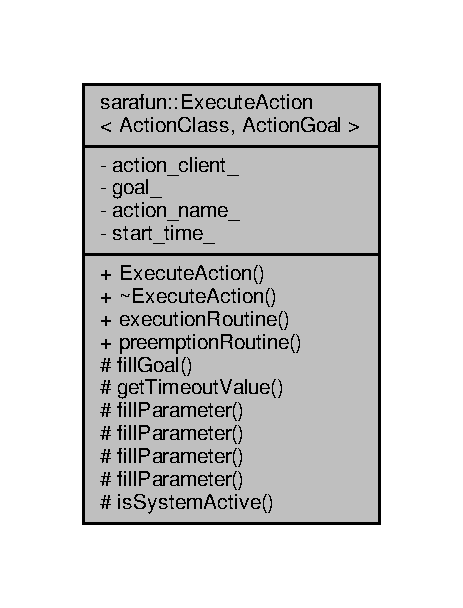
\includegraphics[width=222pt]{de/dc6/classsarafun_1_1ExecuteAction__coll__graph}
\end{center}
\end{figure}
\subsection*{Public Member Functions}
\begin{DoxyCompactItemize}
\item 
\hyperlink{classsarafun_1_1ExecuteAction_acbe4336af2941a52a96aaaceb7e801cb_acbe4336af2941a52a96aaaceb7e801cb}{Execute\-Action} (std\-::string node\-\_\-name, std\-::string actionlib\-\_\-name, std\-::string bt\-\_\-name)
\item 
virtual \hyperlink{classsarafun_1_1ExecuteAction_a194ac46f85d7c70c0aa4f09a0c2941ae_a194ac46f85d7c70c0aa4f09a0c2941ae}{$\sim$\-Execute\-Action} ()
\item 
int \hyperlink{classsarafun_1_1ExecuteAction_ae5e3d1f2779c12923ccdc6289ebba25a_ae5e3d1f2779c12923ccdc6289ebba25a}{execution\-Routine} ()
\item 
void \hyperlink{classsarafun_1_1ExecuteAction_a4075792022071239c6e335c32c70ad2e_a4075792022071239c6e335c32c70ad2e}{preemption\-Routine} ()
\end{DoxyCompactItemize}
\subsection*{Protected Member Functions}
\begin{DoxyCompactItemize}
\item 
virtual bool \hyperlink{classsarafun_1_1ExecuteAction_a6dd9c0f013d15a17d7e7ce8dbe40a436_a6dd9c0f013d15a17d7e7ce8dbe40a436}{fill\-Goal} (Action\-Goal \&goal)=0
\item 
virtual double \hyperlink{classsarafun_1_1ExecuteAction_aba6cfa8a8ce19e735eb6394424df6d17_aba6cfa8a8ce19e735eb6394424df6d17}{get\-Timeout\-Value} ()=0
\item 
bool \hyperlink{classsarafun_1_1ExecuteAction_ac1c8c1ac7392b0ebc8d095d6f6d336e3_ac1c8c1ac7392b0ebc8d095d6f6d336e3}{fill\-Parameter} (std\-::string param\-\_\-name, std\-::string \&param\-\_\-val)
\item 
void \hyperlink{classsarafun_1_1ExecuteAction_a78aa73f154cebe28d4c2fa11ec6a07cf_a78aa73f154cebe28d4c2fa11ec6a07cf}{fill\-Parameter} (std\-::string param\-\_\-name, std\-::string def, std\-::string \&param\-\_\-val)
\item 
void \hyperlink{classsarafun_1_1ExecuteAction_a0c5d656feaf29da583e87f8389570e7d_a0c5d656feaf29da583e87f8389570e7d}{fill\-Parameter} (std\-::string param\-\_\-name, double def, double \&param\-\_\-val)
\item 
void \hyperlink{classsarafun_1_1ExecuteAction_a0ab753300e7535025e7d0508335241a6_a0ab753300e7535025e7d0508335241a6}{fill\-Parameter} (std\-::string param\-\_\-name, int def, int \&param\-\_\-val)
\item 
bool \hyperlink{classsarafun_1_1ExecuteAction_ab9adb2cd743cb8e783fe2a927c94232b_ab9adb2cd743cb8e783fe2a927c94232b}{is\-System\-Active} ()
\end{DoxyCompactItemize}
\subsection*{Private Attributes}
\begin{DoxyCompactItemize}
\item 
actionlib\-::\-Simple\-Action\-Client\\*
$<$ Action\-Class $>$ $\ast$ \hyperlink{classsarafun_1_1ExecuteAction_a8f41836853e5a9daa346b90b865fd113_a8f41836853e5a9daa346b90b865fd113}{action\-\_\-client\-\_\-}
\item 
Action\-Goal \hyperlink{classsarafun_1_1ExecuteAction_a31d3f0c6e50b6abeb68ef6d0cb3c8a4a_a31d3f0c6e50b6abeb68ef6d0cb3c8a4a}{goal\-\_\-}
\item 
std\-::string \hyperlink{classsarafun_1_1ExecuteAction_ac2deed790dd2ff6ef7534fb1a500381f_ac2deed790dd2ff6ef7534fb1a500381f}{action\-\_\-name\-\_\-}
\item 
ros\-::\-Time \hyperlink{classsarafun_1_1ExecuteAction_ad7a81f5e505c421c57bc32fa35e3e84f_ad7a81f5e505c421c57bc32fa35e3e84f}{start\-\_\-time\-\_\-}
\end{DoxyCompactItemize}


\subsection{Detailed Description}
\subsubsection*{template$<$class Action\-Class, class Action\-Goal$>$class sarafun\-::\-Execute\-Action$<$ Action\-Class, Action\-Goal $>$}

This class implements an interface for B\-T actions destined to call a generic rosaction server.

It establishes a bridge between the behavior tree action class and an externally implemented action\-: B\-T $<$--$>$ \hyperlink{classsarafun_1_1ExecuteAction}{Execute\-Action} $<$--$>$ external implementation 

Definition at line 17 of file Execute\-Action.\-h.



\subsection{Constructor \& Destructor Documentation}
\hypertarget{classsarafun_1_1ExecuteAction_acbe4336af2941a52a96aaaceb7e801cb_acbe4336af2941a52a96aaaceb7e801cb}{\index{sarafun\-::\-Execute\-Action@{sarafun\-::\-Execute\-Action}!Execute\-Action@{Execute\-Action}}
\index{Execute\-Action@{Execute\-Action}!sarafun::ExecuteAction@{sarafun\-::\-Execute\-Action}}
\subsubsection[{Execute\-Action}]{\setlength{\rightskip}{0pt plus 5cm}template$<$class Action\-Class , class Action\-Goal $>$ {\bf sarafun\-::\-Execute\-Action}$<$ Action\-Class, Action\-Goal $>$\-::{\bf Execute\-Action} (
\begin{DoxyParamCaption}
\item[{std\-::string}]{node\-\_\-name, }
\item[{std\-::string}]{actionlib\-\_\-name, }
\item[{std\-::string}]{bt\-\_\-name}
\end{DoxyParamCaption}
)}}\label{classsarafun_1_1ExecuteAction_acbe4336af2941a52a96aaaceb7e801cb_acbe4336af2941a52a96aaaceb7e801cb}
Contructor.


\begin{DoxyParams}{Parameters}
{\em node\-\_\-name} & The R\-O\-S node name. \\
\hline
{\em actionlib\-\_\-name} & The actionlib server name that this action will call. \\
\hline
{\em bt\-\_\-name} & The name defined in the \char`\"{}name\char`\"{} tag from the B\-T J\-S\-O\-N input file. \\
\hline
\end{DoxyParams}


Definition at line 90 of file Execute\-Action.\-h.



References sarafun\-::\-Execute\-Action$<$ Action\-Class, Action\-Goal $>$\-::action\-\_\-client\-\_\-, and sarafun\-::\-Execute\-Action$<$ Action\-Class, Action\-Goal $>$\-::action\-\_\-name\-\_\-.

\hypertarget{classsarafun_1_1ExecuteAction_a194ac46f85d7c70c0aa4f09a0c2941ae_a194ac46f85d7c70c0aa4f09a0c2941ae}{\index{sarafun\-::\-Execute\-Action@{sarafun\-::\-Execute\-Action}!$\sim$\-Execute\-Action@{$\sim$\-Execute\-Action}}
\index{$\sim$\-Execute\-Action@{$\sim$\-Execute\-Action}!sarafun::ExecuteAction@{sarafun\-::\-Execute\-Action}}
\subsubsection[{$\sim$\-Execute\-Action}]{\setlength{\rightskip}{0pt plus 5cm}template$<$class Action\-Class , class Action\-Goal $>$ {\bf sarafun\-::\-Execute\-Action}$<$ Action\-Class, Action\-Goal $>$\-::$\sim${\bf Execute\-Action} (
\begin{DoxyParamCaption}
{}
\end{DoxyParamCaption}
)\hspace{0.3cm}{\ttfamily [virtual]}}}\label{classsarafun_1_1ExecuteAction_a194ac46f85d7c70c0aa4f09a0c2941ae_a194ac46f85d7c70c0aa4f09a0c2941ae}


Definition at line 99 of file Execute\-Action.\-h.



\subsection{Member Function Documentation}
\hypertarget{classsarafun_1_1ExecuteAction_ae5e3d1f2779c12923ccdc6289ebba25a_ae5e3d1f2779c12923ccdc6289ebba25a}{\index{sarafun\-::\-Execute\-Action@{sarafun\-::\-Execute\-Action}!execution\-Routine@{execution\-Routine}}
\index{execution\-Routine@{execution\-Routine}!sarafun::ExecuteAction@{sarafun\-::\-Execute\-Action}}
\subsubsection[{execution\-Routine}]{\setlength{\rightskip}{0pt plus 5cm}template$<$class Action\-Class , class Action\-Goal $>$ int {\bf sarafun\-::\-Execute\-Action}$<$ Action\-Class, Action\-Goal $>$\-::execution\-Routine (
\begin{DoxyParamCaption}
{}
\end{DoxyParamCaption}
)}}\label{classsarafun_1_1ExecuteAction_ae5e3d1f2779c12923ccdc6289ebba25a_ae5e3d1f2779c12923ccdc6289ebba25a}


Definition at line 128 of file Execute\-Action.\-h.

\hypertarget{classsarafun_1_1ExecuteAction_a6dd9c0f013d15a17d7e7ce8dbe40a436_a6dd9c0f013d15a17d7e7ce8dbe40a436}{\index{sarafun\-::\-Execute\-Action@{sarafun\-::\-Execute\-Action}!fill\-Goal@{fill\-Goal}}
\index{fill\-Goal@{fill\-Goal}!sarafun::ExecuteAction@{sarafun\-::\-Execute\-Action}}
\subsubsection[{fill\-Goal}]{\setlength{\rightskip}{0pt plus 5cm}template$<$class Action\-Class, class Action\-Goal$>$ virtual bool {\bf sarafun\-::\-Execute\-Action}$<$ Action\-Class, Action\-Goal $>$\-::fill\-Goal (
\begin{DoxyParamCaption}
\item[{Action\-Goal \&}]{goal}
\end{DoxyParamCaption}
)\hspace{0.3cm}{\ttfamily [protected]}, {\ttfamily [pure virtual]}}}\label{classsarafun_1_1ExecuteAction_a6dd9c0f013d15a17d7e7ce8dbe40a436_a6dd9c0f013d15a17d7e7ce8dbe40a436}
Fills in the goal for a particular action.


\begin{DoxyParams}{Parameters}
{\em goal} & The actionlib goal message of the externally implemented action. \\
\hline
\end{DoxyParams}
\begin{DoxyReturn}{Returns}
False in case of error, true otherwise. 
\end{DoxyReturn}


Implemented in \hyperlink{classsarafun_1_1ApproachObjectsAction_af5d216551122da780bc550daf4f1dca4_af5d216551122da780bc550daf4f1dca4}{sarafun\-::\-Approach\-Objects\-Action}, \hyperlink{classsarafun_1_1InsertionWithDeformationAction_a32d695dfcd626c5a7ca0fa987c245083_a32d695dfcd626c5a7ca0fa987c245083}{sarafun\-::\-Insertion\-With\-Deformation\-Action}, \hyperlink{classsarafun_1_1AlignAction_ab92a62085ebd60438638b7b6c56da786_ab92a62085ebd60438638b7b6c56da786}{sarafun\-::\-Align\-Action}, \hyperlink{classsarafun_1_1AssembledAction_a094a5cfde4d6bb6d024256834e771a39_a094a5cfde4d6bb6d024256834e771a39}{sarafun\-::\-Assembled\-Action}, \hyperlink{classsarafun_1_1ContactAction_a563907411debe223088ef5a34d8c0fb0_a563907411debe223088ef5a34d8c0fb0}{sarafun\-::\-Contact\-Action}, \hyperlink{classsarafun_1_1GraspAction_a7418fe9de5024a8fbbfe8e5f5336d66f_a7418fe9de5024a8fbbfe8e5f5336d66f}{sarafun\-::\-Grasp\-Action}, \hyperlink{classsarafun_1_1InitialAction_aac7f439c30455349e075e91542565a43_aac7f439c30455349e075e91542565a43}{sarafun\-::\-Initial\-Action}, \hyperlink{classsarafun_1_1MoveAction_ad5259389b6a5718389c24fab920c9296_ad5259389b6a5718389c24fab920c9296}{sarafun\-::\-Move\-Action}, \hyperlink{classsarafun_1_1PickupAction_a4aa9956733de9f12b52aa41038dbe87a_a4aa9956733de9f12b52aa41038dbe87a}{sarafun\-::\-Pickup\-Action}, \hyperlink{classsarafun_1_1RetractAction_ad0db1c2615d68603bc972ffa26049a70_ad0db1c2615d68603bc972ffa26049a70}{sarafun\-::\-Retract\-Action}, \hyperlink{classsarafun_1_1GrabObjectAction_a61fe8b0cb93dec244f10d6c5dbee913c_a61fe8b0cb93dec244f10d6c5dbee913c}{sarafun\-::\-Grab\-Object\-Action}, \hyperlink{classsarafun_1_1OnlineMotionAction_aacaa264dad7ba07b5c9a985d66ea48f7_aacaa264dad7ba07b5c9a985d66ea48f7}{sarafun\-::\-Online\-Motion\-Action}, \hyperlink{classsarafun_1_1PlaceAction_a7d48e758adf6cea93fa15409bafda8c8_a7d48e758adf6cea93fa15409bafda8c8}{sarafun\-::\-Place\-Action}, and \hyperlink{classsarafun_1_1FoldingAssemblyAction_a51597860319456f359d03c3e27c2fb96_a51597860319456f359d03c3e27c2fb96}{sarafun\-::\-Folding\-Assembly\-Action}.

\hypertarget{classsarafun_1_1ExecuteAction_ac1c8c1ac7392b0ebc8d095d6f6d336e3_ac1c8c1ac7392b0ebc8d095d6f6d336e3}{\index{sarafun\-::\-Execute\-Action@{sarafun\-::\-Execute\-Action}!fill\-Parameter@{fill\-Parameter}}
\index{fill\-Parameter@{fill\-Parameter}!sarafun::ExecuteAction@{sarafun\-::\-Execute\-Action}}
\subsubsection[{fill\-Parameter}]{\setlength{\rightskip}{0pt plus 5cm}template$<$class Action\-Class , class Action\-Goal $>$ bool {\bf sarafun\-::\-Execute\-Action}$<$ Action\-Class, Action\-Goal $>$\-::fill\-Parameter (
\begin{DoxyParamCaption}
\item[{std\-::string}]{param\-\_\-name, }
\item[{std\-::string \&}]{param\-\_\-val}
\end{DoxyParamCaption}
)\hspace{0.3cm}{\ttfamily [protected]}}}\label{classsarafun_1_1ExecuteAction_ac1c8c1ac7392b0ebc8d095d6f6d336e3_ac1c8c1ac7392b0ebc8d095d6f6d336e3}
Gets generic parameter from the parameter server.


\begin{DoxyParams}{Parameters}
{\em The} & parameter name.  The parameter value. \\
\hline
\end{DoxyParams}
\begin{DoxyReturn}{Returns}
False in case the parameter does not exist, true otherise. 
\end{DoxyReturn}


Definition at line 198 of file Execute\-Action.\-h.

\hypertarget{classsarafun_1_1ExecuteAction_a78aa73f154cebe28d4c2fa11ec6a07cf_a78aa73f154cebe28d4c2fa11ec6a07cf}{\index{sarafun\-::\-Execute\-Action@{sarafun\-::\-Execute\-Action}!fill\-Parameter@{fill\-Parameter}}
\index{fill\-Parameter@{fill\-Parameter}!sarafun::ExecuteAction@{sarafun\-::\-Execute\-Action}}
\subsubsection[{fill\-Parameter}]{\setlength{\rightskip}{0pt plus 5cm}template$<$class Action\-Class , class Action\-Goal $>$ void {\bf sarafun\-::\-Execute\-Action}$<$ Action\-Class, Action\-Goal $>$\-::fill\-Parameter (
\begin{DoxyParamCaption}
\item[{std\-::string}]{param\-\_\-name, }
\item[{std\-::string}]{def, }
\item[{std\-::string \&}]{param\-\_\-val}
\end{DoxyParamCaption}
)\hspace{0.3cm}{\ttfamily [protected]}}}\label{classsarafun_1_1ExecuteAction_a78aa73f154cebe28d4c2fa11ec6a07cf_a78aa73f154cebe28d4c2fa11ec6a07cf}
Gets a generic parameter from the parameter server. Sets it to a default in case the parameter does not exist.


\begin{DoxyParams}{Parameters}
{\em The} & parameter name \\
\hline
{\em def} & The default parameter value  The parameter value \\
\hline
\end{DoxyParams}


Definition at line 210 of file Execute\-Action.\-h.

\hypertarget{classsarafun_1_1ExecuteAction_a0c5d656feaf29da583e87f8389570e7d_a0c5d656feaf29da583e87f8389570e7d}{\index{sarafun\-::\-Execute\-Action@{sarafun\-::\-Execute\-Action}!fill\-Parameter@{fill\-Parameter}}
\index{fill\-Parameter@{fill\-Parameter}!sarafun::ExecuteAction@{sarafun\-::\-Execute\-Action}}
\subsubsection[{fill\-Parameter}]{\setlength{\rightskip}{0pt plus 5cm}template$<$class Action\-Class , class Action\-Goal $>$ void {\bf sarafun\-::\-Execute\-Action}$<$ Action\-Class, Action\-Goal $>$\-::fill\-Parameter (
\begin{DoxyParamCaption}
\item[{std\-::string}]{param\-\_\-name, }
\item[{double}]{def, }
\item[{double \&}]{param\-\_\-val}
\end{DoxyParamCaption}
)\hspace{0.3cm}{\ttfamily [protected]}}}\label{classsarafun_1_1ExecuteAction_a0c5d656feaf29da583e87f8389570e7d_a0c5d656feaf29da583e87f8389570e7d}


Definition at line 221 of file Execute\-Action.\-h.

\hypertarget{classsarafun_1_1ExecuteAction_a0ab753300e7535025e7d0508335241a6_a0ab753300e7535025e7d0508335241a6}{\index{sarafun\-::\-Execute\-Action@{sarafun\-::\-Execute\-Action}!fill\-Parameter@{fill\-Parameter}}
\index{fill\-Parameter@{fill\-Parameter}!sarafun::ExecuteAction@{sarafun\-::\-Execute\-Action}}
\subsubsection[{fill\-Parameter}]{\setlength{\rightskip}{0pt plus 5cm}template$<$class Action\-Class , class Action\-Goal $>$ void {\bf sarafun\-::\-Execute\-Action}$<$ Action\-Class, Action\-Goal $>$\-::fill\-Parameter (
\begin{DoxyParamCaption}
\item[{std\-::string}]{param\-\_\-name, }
\item[{int}]{def, }
\item[{int \&}]{param\-\_\-val}
\end{DoxyParamCaption}
)\hspace{0.3cm}{\ttfamily [protected]}}}\label{classsarafun_1_1ExecuteAction_a0ab753300e7535025e7d0508335241a6_a0ab753300e7535025e7d0508335241a6}


Definition at line 232 of file Execute\-Action.\-h.

\hypertarget{classsarafun_1_1ExecuteAction_aba6cfa8a8ce19e735eb6394424df6d17_aba6cfa8a8ce19e735eb6394424df6d17}{\index{sarafun\-::\-Execute\-Action@{sarafun\-::\-Execute\-Action}!get\-Timeout\-Value@{get\-Timeout\-Value}}
\index{get\-Timeout\-Value@{get\-Timeout\-Value}!sarafun::ExecuteAction@{sarafun\-::\-Execute\-Action}}
\subsubsection[{get\-Timeout\-Value}]{\setlength{\rightskip}{0pt plus 5cm}template$<$class Action\-Class, class Action\-Goal$>$ virtual double {\bf sarafun\-::\-Execute\-Action}$<$ Action\-Class, Action\-Goal $>$\-::get\-Timeout\-Value (
\begin{DoxyParamCaption}
{}
\end{DoxyParamCaption}
)\hspace{0.3cm}{\ttfamily [protected]}, {\ttfamily [pure virtual]}}}\label{classsarafun_1_1ExecuteAction_aba6cfa8a8ce19e735eb6394424df6d17_aba6cfa8a8ce19e735eb6394424df6d17}
Provides the client with a timeout value for actionlib connections.

\begin{DoxyReturn}{Returns}
The timeout value (in seconds). 
\end{DoxyReturn}


Implemented in \hyperlink{classsarafun_1_1ApproachObjectsAction_a6852994a6e8a1edf9b2c24c91fd07df2_a6852994a6e8a1edf9b2c24c91fd07df2}{sarafun\-::\-Approach\-Objects\-Action}, \hyperlink{classsarafun_1_1InsertionWithDeformationAction_a8d77b104fb2396000b273cb6754ff879_a8d77b104fb2396000b273cb6754ff879}{sarafun\-::\-Insertion\-With\-Deformation\-Action}, \hyperlink{classsarafun_1_1AlignAction_a9b9741ec3203bdc1b2e7b7cecc96e6ed_a9b9741ec3203bdc1b2e7b7cecc96e6ed}{sarafun\-::\-Align\-Action}, \hyperlink{classsarafun_1_1AssembledAction_ade9095a291dce652339238d137419b49_ade9095a291dce652339238d137419b49}{sarafun\-::\-Assembled\-Action}, \hyperlink{classsarafun_1_1ContactAction_a85d81232d228fc6d2856d318d25c1bf9_a85d81232d228fc6d2856d318d25c1bf9}{sarafun\-::\-Contact\-Action}, \hyperlink{classsarafun_1_1GraspAction_a406d5c86b5f788537c5af9d125724a55_a406d5c86b5f788537c5af9d125724a55}{sarafun\-::\-Grasp\-Action}, \hyperlink{classsarafun_1_1InitialAction_a1b58c06c32ec9f9d3e75c37de5e7d2c8_a1b58c06c32ec9f9d3e75c37de5e7d2c8}{sarafun\-::\-Initial\-Action}, \hyperlink{classsarafun_1_1MoveAction_a3a0d4d2919b30b878c603a884db6a470_a3a0d4d2919b30b878c603a884db6a470}{sarafun\-::\-Move\-Action}, \hyperlink{classsarafun_1_1PickupAction_a02643cdc836095102e5622b660233f26_a02643cdc836095102e5622b660233f26}{sarafun\-::\-Pickup\-Action}, \hyperlink{classsarafun_1_1RetractAction_af95bb8d3826dbe1444a8a3e12d8596b0_af95bb8d3826dbe1444a8a3e12d8596b0}{sarafun\-::\-Retract\-Action}, \hyperlink{classsarafun_1_1GrabObjectAction_a6e2ee834fda8bd8d0dbdc101c8acdd9c_a6e2ee834fda8bd8d0dbdc101c8acdd9c}{sarafun\-::\-Grab\-Object\-Action}, \hyperlink{classsarafun_1_1OnlineMotionAction_a453e7dca41a0d73b5297ce191e760b31_a453e7dca41a0d73b5297ce191e760b31}{sarafun\-::\-Online\-Motion\-Action}, \hyperlink{classsarafun_1_1PlaceAction_a0b53372fd2de920c3ebd94c8c7f80b6a_a0b53372fd2de920c3ebd94c8c7f80b6a}{sarafun\-::\-Place\-Action}, and \hyperlink{classsarafun_1_1FoldingAssemblyAction_a14174e375aa1b8d5b63159f275b7d971_a14174e375aa1b8d5b63159f275b7d971}{sarafun\-::\-Folding\-Assembly\-Action}.

\hypertarget{classsarafun_1_1ExecuteAction_ab9adb2cd743cb8e783fe2a927c94232b_ab9adb2cd743cb8e783fe2a927c94232b}{\index{sarafun\-::\-Execute\-Action@{sarafun\-::\-Execute\-Action}!is\-System\-Active@{is\-System\-Active}}
\index{is\-System\-Active@{is\-System\-Active}!sarafun::ExecuteAction@{sarafun\-::\-Execute\-Action}}
\subsubsection[{is\-System\-Active}]{\setlength{\rightskip}{0pt plus 5cm}template$<$class Action\-Class , class Action\-Goal $>$ bool {\bf sarafun\-::\-Execute\-Action}$<$ Action\-Class, Action\-Goal $>$\-::is\-System\-Active (
\begin{DoxyParamCaption}
{}
\end{DoxyParamCaption}
)\hspace{0.3cm}{\ttfamily [protected]}}}\label{classsarafun_1_1ExecuteAction_ab9adb2cd743cb8e783fe2a927c94232b_ab9adb2cd743cb8e783fe2a927c94232b}
Checks if B\-T action execution is allowed.

\begin{DoxyReturn}{Returns}
True if the tree is active, false otherwise. 
\end{DoxyReturn}


Definition at line 104 of file Execute\-Action.\-h.

\hypertarget{classsarafun_1_1ExecuteAction_a4075792022071239c6e335c32c70ad2e_a4075792022071239c6e335c32c70ad2e}{\index{sarafun\-::\-Execute\-Action@{sarafun\-::\-Execute\-Action}!preemption\-Routine@{preemption\-Routine}}
\index{preemption\-Routine@{preemption\-Routine}!sarafun::ExecuteAction@{sarafun\-::\-Execute\-Action}}
\subsubsection[{preemption\-Routine}]{\setlength{\rightskip}{0pt plus 5cm}template$<$class Action\-Class , class Action\-Goal $>$ void {\bf sarafun\-::\-Execute\-Action}$<$ Action\-Class, Action\-Goal $>$\-::preemption\-Routine (
\begin{DoxyParamCaption}
{}
\end{DoxyParamCaption}
)}}\label{classsarafun_1_1ExecuteAction_a4075792022071239c6e335c32c70ad2e_a4075792022071239c6e335c32c70ad2e}


Definition at line 120 of file Execute\-Action.\-h.



\subsection{Field Documentation}
\hypertarget{classsarafun_1_1ExecuteAction_a8f41836853e5a9daa346b90b865fd113_a8f41836853e5a9daa346b90b865fd113}{\index{sarafun\-::\-Execute\-Action@{sarafun\-::\-Execute\-Action}!action\-\_\-client\-\_\-@{action\-\_\-client\-\_\-}}
\index{action\-\_\-client\-\_\-@{action\-\_\-client\-\_\-}!sarafun::ExecuteAction@{sarafun\-::\-Execute\-Action}}
\subsubsection[{action\-\_\-client\-\_\-}]{\setlength{\rightskip}{0pt plus 5cm}template$<$class Action\-Class, class Action\-Goal$>$ actionlib\-::\-Simple\-Action\-Client$<$Action\-Class$>$$\ast$ {\bf sarafun\-::\-Execute\-Action}$<$ Action\-Class, Action\-Goal $>$\-::action\-\_\-client\-\_\-\hspace{0.3cm}{\ttfamily [private]}}}\label{classsarafun_1_1ExecuteAction_a8f41836853e5a9daa346b90b865fd113_a8f41836853e5a9daa346b90b865fd113}


Definition at line 80 of file Execute\-Action.\-h.



Referenced by sarafun\-::\-Execute\-Action$<$ Action\-Class, Action\-Goal $>$\-::\-Execute\-Action().

\hypertarget{classsarafun_1_1ExecuteAction_ac2deed790dd2ff6ef7534fb1a500381f_ac2deed790dd2ff6ef7534fb1a500381f}{\index{sarafun\-::\-Execute\-Action@{sarafun\-::\-Execute\-Action}!action\-\_\-name\-\_\-@{action\-\_\-name\-\_\-}}
\index{action\-\_\-name\-\_\-@{action\-\_\-name\-\_\-}!sarafun::ExecuteAction@{sarafun\-::\-Execute\-Action}}
\subsubsection[{action\-\_\-name\-\_\-}]{\setlength{\rightskip}{0pt plus 5cm}template$<$class Action\-Class, class Action\-Goal$>$ std\-::string {\bf sarafun\-::\-Execute\-Action}$<$ Action\-Class, Action\-Goal $>$\-::action\-\_\-name\-\_\-\hspace{0.3cm}{\ttfamily [private]}}}\label{classsarafun_1_1ExecuteAction_ac2deed790dd2ff6ef7534fb1a500381f_ac2deed790dd2ff6ef7534fb1a500381f}


Definition at line 82 of file Execute\-Action.\-h.



Referenced by sarafun\-::\-Execute\-Action$<$ Action\-Class, Action\-Goal $>$\-::\-Execute\-Action().

\hypertarget{classsarafun_1_1ExecuteAction_a31d3f0c6e50b6abeb68ef6d0cb3c8a4a_a31d3f0c6e50b6abeb68ef6d0cb3c8a4a}{\index{sarafun\-::\-Execute\-Action@{sarafun\-::\-Execute\-Action}!goal\-\_\-@{goal\-\_\-}}
\index{goal\-\_\-@{goal\-\_\-}!sarafun::ExecuteAction@{sarafun\-::\-Execute\-Action}}
\subsubsection[{goal\-\_\-}]{\setlength{\rightskip}{0pt plus 5cm}template$<$class Action\-Class, class Action\-Goal$>$ Action\-Goal {\bf sarafun\-::\-Execute\-Action}$<$ Action\-Class, Action\-Goal $>$\-::goal\-\_\-\hspace{0.3cm}{\ttfamily [private]}}}\label{classsarafun_1_1ExecuteAction_a31d3f0c6e50b6abeb68ef6d0cb3c8a4a_a31d3f0c6e50b6abeb68ef6d0cb3c8a4a}


Definition at line 81 of file Execute\-Action.\-h.

\hypertarget{classsarafun_1_1ExecuteAction_ad7a81f5e505c421c57bc32fa35e3e84f_ad7a81f5e505c421c57bc32fa35e3e84f}{\index{sarafun\-::\-Execute\-Action@{sarafun\-::\-Execute\-Action}!start\-\_\-time\-\_\-@{start\-\_\-time\-\_\-}}
\index{start\-\_\-time\-\_\-@{start\-\_\-time\-\_\-}!sarafun::ExecuteAction@{sarafun\-::\-Execute\-Action}}
\subsubsection[{start\-\_\-time\-\_\-}]{\setlength{\rightskip}{0pt plus 5cm}template$<$class Action\-Class, class Action\-Goal$>$ ros\-::\-Time {\bf sarafun\-::\-Execute\-Action}$<$ Action\-Class, Action\-Goal $>$\-::start\-\_\-time\-\_\-\hspace{0.3cm}{\ttfamily [private]}}}\label{classsarafun_1_1ExecuteAction_ad7a81f5e505c421c57bc32fa35e3e84f_ad7a81f5e505c421c57bc32fa35e3e84f}


Definition at line 83 of file Execute\-Action.\-h.



The documentation for this class was generated from the following file\-:\begin{DoxyCompactItemize}
\item 
Execute\-Action.\-h\end{DoxyCompactItemize}

\hypertarget{classsarafun_1_1FoldingAssemblyAction}{\section{sarafun\-:\-:Folding\-Assembly\-Action Class Reference}
\label{classsarafun_1_1FoldingAssemblyAction}\index{sarafun\-::\-Folding\-Assembly\-Action@{sarafun\-::\-Folding\-Assembly\-Action}}
}


{\ttfamily \#include $<$Folding\-Assembly\-Action.\-h$>$}



Inheritance diagram for sarafun\-:\-:Folding\-Assembly\-Action\-:
\nopagebreak
\begin{figure}[H]
\begin{center}
\leavevmode
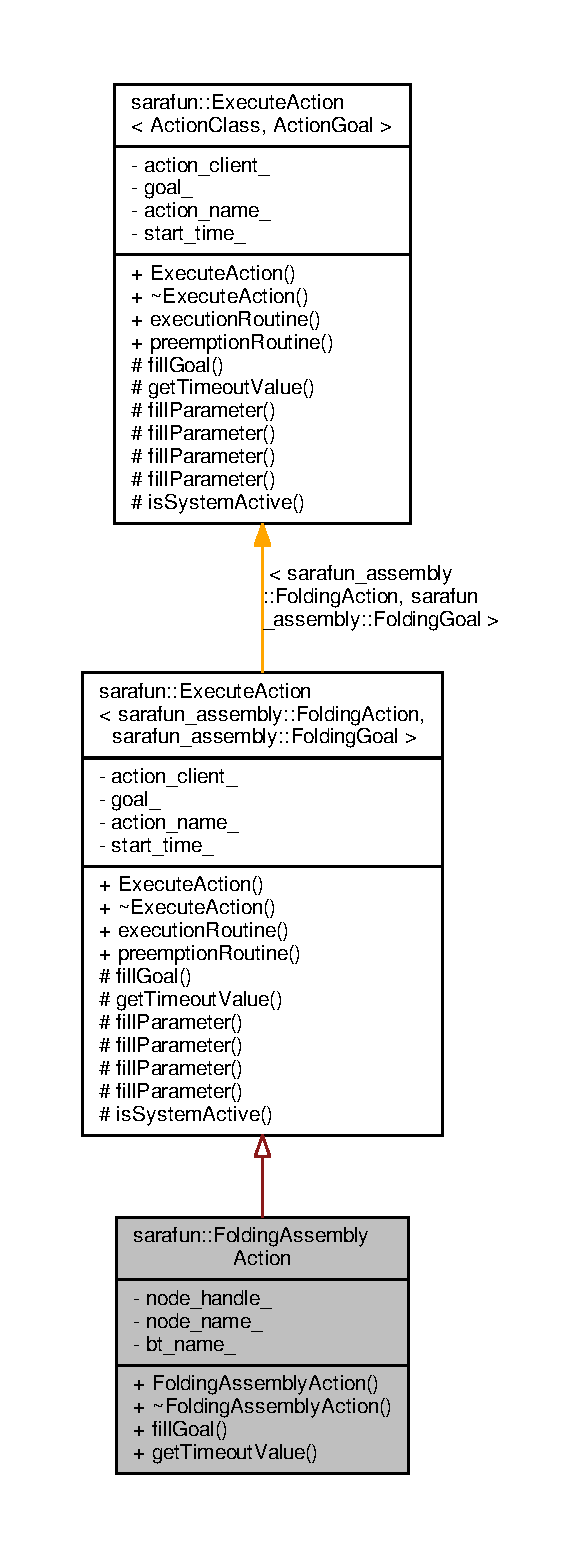
\includegraphics[height=550pt]{d3/d87/classsarafun_1_1FoldingAssemblyAction__inherit__graph}
\end{center}
\end{figure}


Collaboration diagram for sarafun\-:\-:Folding\-Assembly\-Action\-:
\nopagebreak
\begin{figure}[H]
\begin{center}
\leavevmode
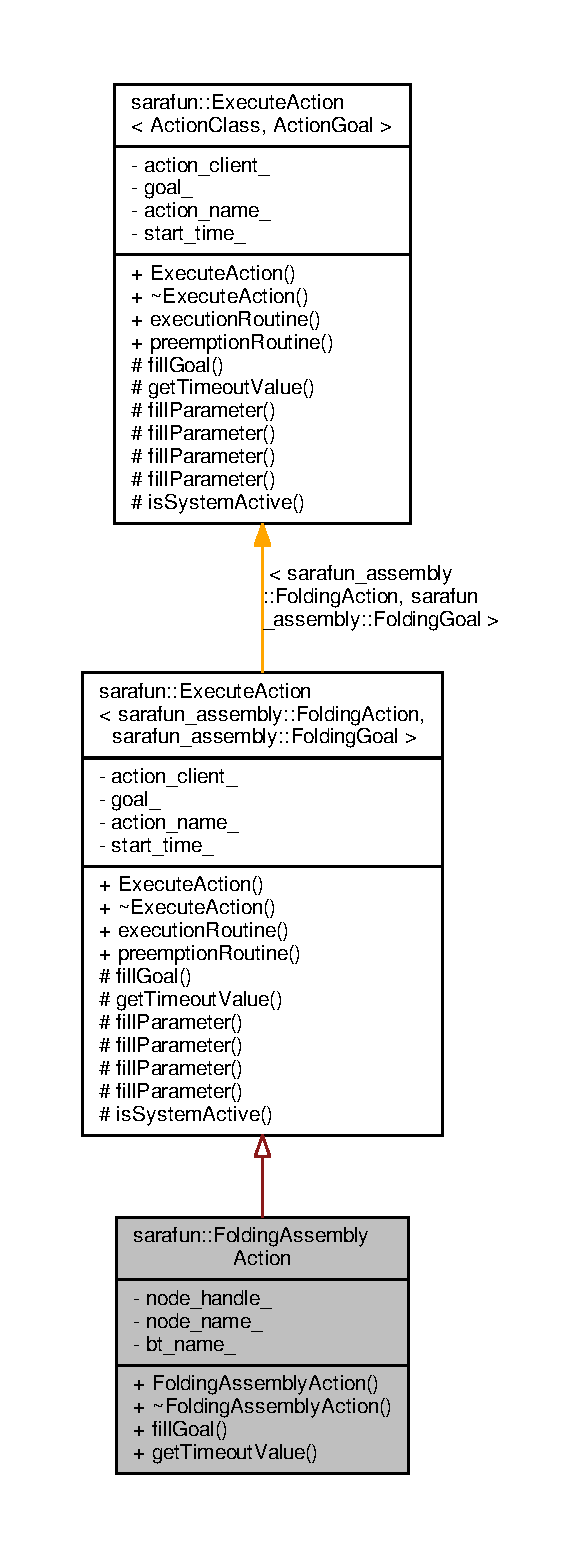
\includegraphics[height=550pt]{de/d2e/classsarafun_1_1FoldingAssemblyAction__coll__graph}
\end{center}
\end{figure}
\subsection*{Public Member Functions}
\begin{DoxyCompactItemize}
\item 
\hyperlink{classsarafun_1_1FoldingAssemblyAction_afc2da251f362a62c892f41d8e0bea0e5_afc2da251f362a62c892f41d8e0bea0e5}{Folding\-Assembly\-Action} (std\-::string node\-\_\-name, std\-::string action\-\_\-name, std\-::string bt\-\_\-name)
\item 
\hyperlink{classsarafun_1_1FoldingAssemblyAction_a0e38e473ec7b9327dc0a4d32e11cc0d6_a0e38e473ec7b9327dc0a4d32e11cc0d6}{$\sim$\-Folding\-Assembly\-Action} ()
\item 
bool \hyperlink{classsarafun_1_1FoldingAssemblyAction_a51597860319456f359d03c3e27c2fb96_a51597860319456f359d03c3e27c2fb96}{fill\-Goal} (sarafun\-\_\-assembly\-::\-Folding\-Goal \&goal)
\item 
double \hyperlink{classsarafun_1_1FoldingAssemblyAction_a14174e375aa1b8d5b63159f275b7d971_a14174e375aa1b8d5b63159f275b7d971}{get\-Timeout\-Value} ()
\end{DoxyCompactItemize}
\subsection*{Private Attributes}
\begin{DoxyCompactItemize}
\item 
ros\-::\-Node\-Handle \hyperlink{classsarafun_1_1FoldingAssemblyAction_a93ef41f7c8fe0fff59227e01deae7625_a93ef41f7c8fe0fff59227e01deae7625}{node\-\_\-handle\-\_\-}
\item 
std\-::string \hyperlink{classsarafun_1_1FoldingAssemblyAction_a80098bc35b0c446a61b0e84f4e97c8ab_a80098bc35b0c446a61b0e84f4e97c8ab}{node\-\_\-name\-\_\-}
\item 
std\-::string \hyperlink{classsarafun_1_1FoldingAssemblyAction_a058ad644052e931e604053b6064f7576_a058ad644052e931e604053b6064f7576}{bt\-\_\-name\-\_\-}
\end{DoxyCompactItemize}
\subsection*{Additional Inherited Members}


\subsection{Detailed Description}


Definition at line 9 of file Folding\-Assembly\-Action.\-h.



\subsection{Constructor \& Destructor Documentation}
\hypertarget{classsarafun_1_1FoldingAssemblyAction_afc2da251f362a62c892f41d8e0bea0e5_afc2da251f362a62c892f41d8e0bea0e5}{\index{sarafun\-::\-Folding\-Assembly\-Action@{sarafun\-::\-Folding\-Assembly\-Action}!Folding\-Assembly\-Action@{Folding\-Assembly\-Action}}
\index{Folding\-Assembly\-Action@{Folding\-Assembly\-Action}!sarafun::FoldingAssemblyAction@{sarafun\-::\-Folding\-Assembly\-Action}}
\subsubsection[{Folding\-Assembly\-Action}]{\setlength{\rightskip}{0pt plus 5cm}sarafun\-::\-Folding\-Assembly\-Action\-::\-Folding\-Assembly\-Action (
\begin{DoxyParamCaption}
\item[{std\-::string}]{node\-\_\-name, }
\item[{std\-::string}]{action\-\_\-name, }
\item[{std\-::string}]{bt\-\_\-name}
\end{DoxyParamCaption}
)\hspace{0.3cm}{\ttfamily [inline]}}}\label{classsarafun_1_1FoldingAssemblyAction_afc2da251f362a62c892f41d8e0bea0e5_afc2da251f362a62c892f41d8e0bea0e5}


Definition at line 12 of file Folding\-Assembly\-Action.\-h.



References node\-\_\-handle\-\_\-.

\hypertarget{classsarafun_1_1FoldingAssemblyAction_a0e38e473ec7b9327dc0a4d32e11cc0d6_a0e38e473ec7b9327dc0a4d32e11cc0d6}{\index{sarafun\-::\-Folding\-Assembly\-Action@{sarafun\-::\-Folding\-Assembly\-Action}!$\sim$\-Folding\-Assembly\-Action@{$\sim$\-Folding\-Assembly\-Action}}
\index{$\sim$\-Folding\-Assembly\-Action@{$\sim$\-Folding\-Assembly\-Action}!sarafun::FoldingAssemblyAction@{sarafun\-::\-Folding\-Assembly\-Action}}
\subsubsection[{$\sim$\-Folding\-Assembly\-Action}]{\setlength{\rightskip}{0pt plus 5cm}sarafun\-::\-Folding\-Assembly\-Action\-::$\sim$\-Folding\-Assembly\-Action (
\begin{DoxyParamCaption}
{}
\end{DoxyParamCaption}
)\hspace{0.3cm}{\ttfamily [inline]}}}\label{classsarafun_1_1FoldingAssemblyAction_a0e38e473ec7b9327dc0a4d32e11cc0d6_a0e38e473ec7b9327dc0a4d32e11cc0d6}


Definition at line 21 of file Folding\-Assembly\-Action.\-h.



\subsection{Member Function Documentation}
\hypertarget{classsarafun_1_1FoldingAssemblyAction_a51597860319456f359d03c3e27c2fb96_a51597860319456f359d03c3e27c2fb96}{\index{sarafun\-::\-Folding\-Assembly\-Action@{sarafun\-::\-Folding\-Assembly\-Action}!fill\-Goal@{fill\-Goal}}
\index{fill\-Goal@{fill\-Goal}!sarafun::FoldingAssemblyAction@{sarafun\-::\-Folding\-Assembly\-Action}}
\subsubsection[{fill\-Goal}]{\setlength{\rightskip}{0pt plus 5cm}bool sarafun\-::\-Folding\-Assembly\-Action\-::fill\-Goal (
\begin{DoxyParamCaption}
\item[{sarafun\-\_\-assembly\-::\-Folding\-Goal \&}]{goal}
\end{DoxyParamCaption}
)\hspace{0.3cm}{\ttfamily [virtual]}}}\label{classsarafun_1_1FoldingAssemblyAction_a51597860319456f359d03c3e27c2fb96_a51597860319456f359d03c3e27c2fb96}
Fills in the goal for a particular action.


\begin{DoxyParams}{Parameters}
{\em goal} & The actionlib goal message of the externally implemented action. \\
\hline
\end{DoxyParams}
\begin{DoxyReturn}{Returns}
False in case of error, true otherwise. 
\end{DoxyReturn}


Implements \hyperlink{classsarafun_1_1ExecuteAction_a6dd9c0f013d15a17d7e7ce8dbe40a436_a6dd9c0f013d15a17d7e7ce8dbe40a436}{sarafun\-::\-Execute\-Action$<$ sarafun\-\_\-assembly\-::\-Folding\-Action, sarafun\-\_\-assembly\-::\-Folding\-Goal $>$}.



Definition at line 11 of file Folding\-Assembly\-Action.\-cpp.

\hypertarget{classsarafun_1_1FoldingAssemblyAction_a14174e375aa1b8d5b63159f275b7d971_a14174e375aa1b8d5b63159f275b7d971}{\index{sarafun\-::\-Folding\-Assembly\-Action@{sarafun\-::\-Folding\-Assembly\-Action}!get\-Timeout\-Value@{get\-Timeout\-Value}}
\index{get\-Timeout\-Value@{get\-Timeout\-Value}!sarafun::FoldingAssemblyAction@{sarafun\-::\-Folding\-Assembly\-Action}}
\subsubsection[{get\-Timeout\-Value}]{\setlength{\rightskip}{0pt plus 5cm}double sarafun\-::\-Folding\-Assembly\-Action\-::get\-Timeout\-Value (
\begin{DoxyParamCaption}
{}
\end{DoxyParamCaption}
)\hspace{0.3cm}{\ttfamily [virtual]}}}\label{classsarafun_1_1FoldingAssemblyAction_a14174e375aa1b8d5b63159f275b7d971_a14174e375aa1b8d5b63159f275b7d971}
Provides the client with a timeout value for actionlib connections.

\begin{DoxyReturn}{Returns}
The timeout value (in seconds). 
\end{DoxyReturn}


Implements \hyperlink{classsarafun_1_1ExecuteAction_aba6cfa8a8ce19e735eb6394424df6d17_aba6cfa8a8ce19e735eb6394424df6d17}{sarafun\-::\-Execute\-Action$<$ sarafun\-\_\-assembly\-::\-Folding\-Action, sarafun\-\_\-assembly\-::\-Folding\-Goal $>$}.



Definition at line 4 of file Folding\-Assembly\-Action.\-cpp.



References sarafun\-::\-Execute\-Action$<$ sarafun\-\_\-assembly\-::\-Folding\-Action, sarafun\-\_\-assembly\-::\-Folding\-Goal $>$\-::fill\-Parameter().



Here is the call graph for this function\-:
\nopagebreak
\begin{figure}[H]
\begin{center}
\leavevmode
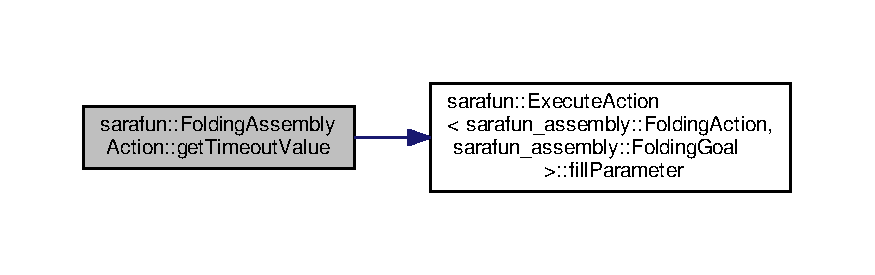
\includegraphics[width=350pt]{dd/df2/classsarafun_1_1FoldingAssemblyAction_a14174e375aa1b8d5b63159f275b7d971_a14174e375aa1b8d5b63159f275b7d971_cgraph}
\end{center}
\end{figure}




\subsection{Field Documentation}
\hypertarget{classsarafun_1_1FoldingAssemblyAction_a058ad644052e931e604053b6064f7576_a058ad644052e931e604053b6064f7576}{\index{sarafun\-::\-Folding\-Assembly\-Action@{sarafun\-::\-Folding\-Assembly\-Action}!bt\-\_\-name\-\_\-@{bt\-\_\-name\-\_\-}}
\index{bt\-\_\-name\-\_\-@{bt\-\_\-name\-\_\-}!sarafun::FoldingAssemblyAction@{sarafun\-::\-Folding\-Assembly\-Action}}
\subsubsection[{bt\-\_\-name\-\_\-}]{\setlength{\rightskip}{0pt plus 5cm}std\-::string sarafun\-::\-Folding\-Assembly\-Action\-::bt\-\_\-name\-\_\-\hspace{0.3cm}{\ttfamily [private]}}}\label{classsarafun_1_1FoldingAssemblyAction_a058ad644052e931e604053b6064f7576_a058ad644052e931e604053b6064f7576}


Definition at line 29 of file Folding\-Assembly\-Action.\-h.

\hypertarget{classsarafun_1_1FoldingAssemblyAction_a93ef41f7c8fe0fff59227e01deae7625_a93ef41f7c8fe0fff59227e01deae7625}{\index{sarafun\-::\-Folding\-Assembly\-Action@{sarafun\-::\-Folding\-Assembly\-Action}!node\-\_\-handle\-\_\-@{node\-\_\-handle\-\_\-}}
\index{node\-\_\-handle\-\_\-@{node\-\_\-handle\-\_\-}!sarafun::FoldingAssemblyAction@{sarafun\-::\-Folding\-Assembly\-Action}}
\subsubsection[{node\-\_\-handle\-\_\-}]{\setlength{\rightskip}{0pt plus 5cm}ros\-::\-Node\-Handle sarafun\-::\-Folding\-Assembly\-Action\-::node\-\_\-handle\-\_\-\hspace{0.3cm}{\ttfamily [private]}}}\label{classsarafun_1_1FoldingAssemblyAction_a93ef41f7c8fe0fff59227e01deae7625_a93ef41f7c8fe0fff59227e01deae7625}


Definition at line 27 of file Folding\-Assembly\-Action.\-h.



Referenced by Folding\-Assembly\-Action().

\hypertarget{classsarafun_1_1FoldingAssemblyAction_a80098bc35b0c446a61b0e84f4e97c8ab_a80098bc35b0c446a61b0e84f4e97c8ab}{\index{sarafun\-::\-Folding\-Assembly\-Action@{sarafun\-::\-Folding\-Assembly\-Action}!node\-\_\-name\-\_\-@{node\-\_\-name\-\_\-}}
\index{node\-\_\-name\-\_\-@{node\-\_\-name\-\_\-}!sarafun::FoldingAssemblyAction@{sarafun\-::\-Folding\-Assembly\-Action}}
\subsubsection[{node\-\_\-name\-\_\-}]{\setlength{\rightskip}{0pt plus 5cm}std\-::string sarafun\-::\-Folding\-Assembly\-Action\-::node\-\_\-name\-\_\-\hspace{0.3cm}{\ttfamily [private]}}}\label{classsarafun_1_1FoldingAssemblyAction_a80098bc35b0c446a61b0e84f4e97c8ab_a80098bc35b0c446a61b0e84f4e97c8ab}


Definition at line 28 of file Folding\-Assembly\-Action.\-h.



The documentation for this class was generated from the following files\-:\begin{DoxyCompactItemize}
\item 
Folding\-Assembly\-Action.\-h\item 
Folding\-Assembly\-Action.\-cpp\end{DoxyCompactItemize}

\hypertarget{classsarafun_1_1GrabObjectAction}{\section{sarafun\-:\-:Grab\-Object\-Action Class Reference}
\label{classsarafun_1_1GrabObjectAction}\index{sarafun\-::\-Grab\-Object\-Action@{sarafun\-::\-Grab\-Object\-Action}}
}


{\ttfamily \#include $<$Grab\-Object\-Action.\-h$>$}



Inheritance diagram for sarafun\-:\-:Grab\-Object\-Action\-:
\nopagebreak
\begin{figure}[H]
\begin{center}
\leavevmode
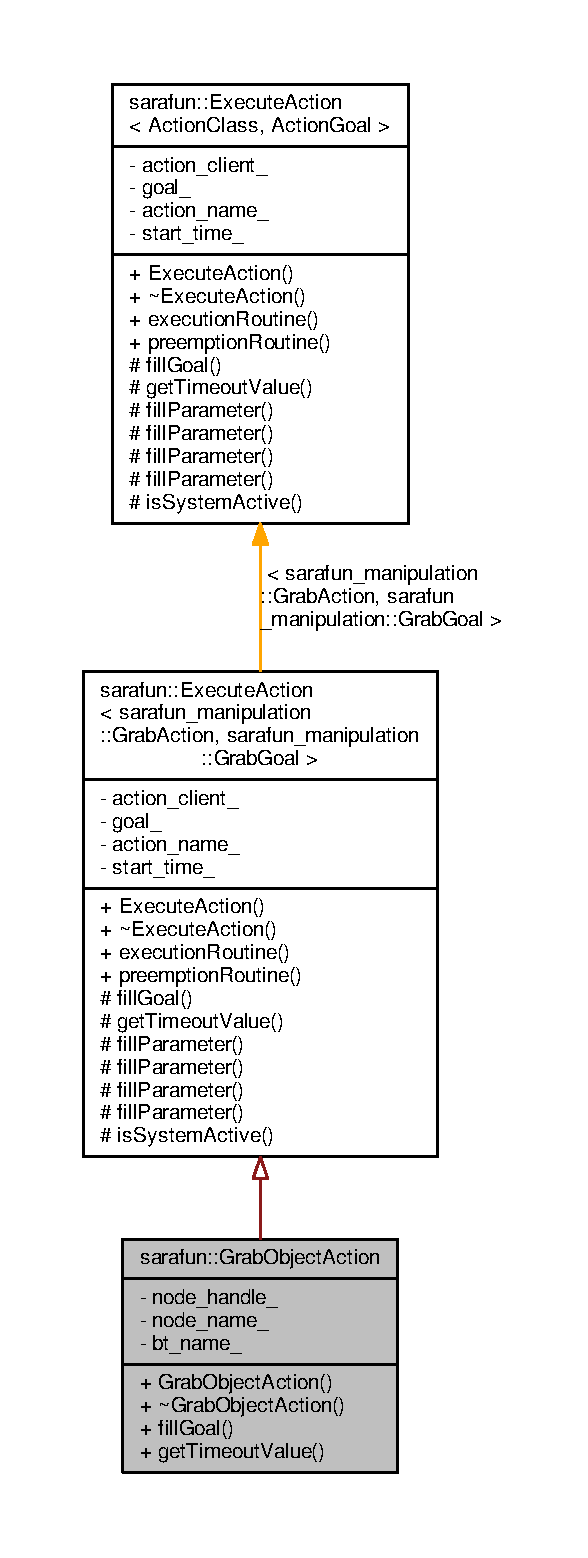
\includegraphics[height=550pt]{db/dc6/classsarafun_1_1GrabObjectAction__inherit__graph}
\end{center}
\end{figure}


Collaboration diagram for sarafun\-:\-:Grab\-Object\-Action\-:
\nopagebreak
\begin{figure}[H]
\begin{center}
\leavevmode
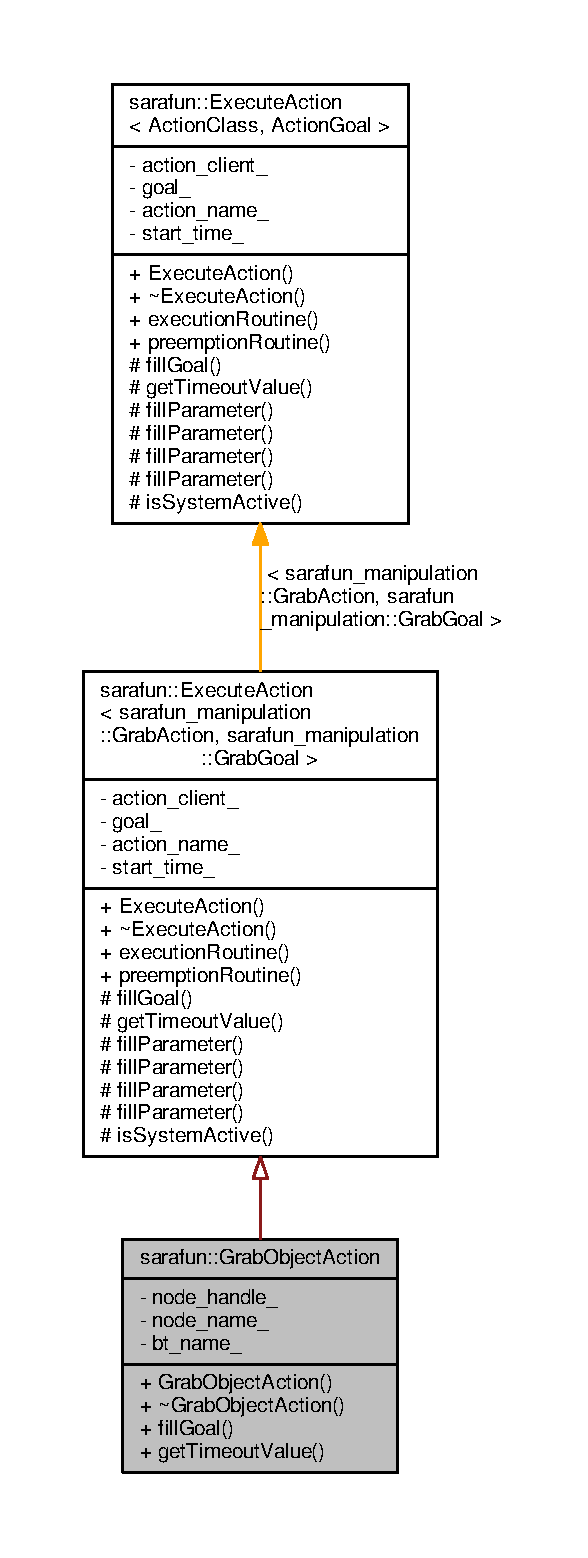
\includegraphics[height=550pt]{d7/d04/classsarafun_1_1GrabObjectAction__coll__graph}
\end{center}
\end{figure}
\subsection*{Public Member Functions}
\begin{DoxyCompactItemize}
\item 
\hyperlink{classsarafun_1_1GrabObjectAction_abca8f2d915cf1a8d507d04885b3e1df9_abca8f2d915cf1a8d507d04885b3e1df9}{Grab\-Object\-Action} (std\-::string node\-\_\-name, std\-::string action\-\_\-name, std\-::string bt\-\_\-name)
\item 
\hyperlink{classsarafun_1_1GrabObjectAction_a1b1ee63f9ba24332b2184b67021dbf0e_a1b1ee63f9ba24332b2184b67021dbf0e}{$\sim$\-Grab\-Object\-Action} ()
\item 
bool \hyperlink{classsarafun_1_1GrabObjectAction_a61fe8b0cb93dec244f10d6c5dbee913c_a61fe8b0cb93dec244f10d6c5dbee913c}{fill\-Goal} (sarafun\-\_\-manipulation\-::\-Grab\-Goal \&goal)
\item 
double \hyperlink{classsarafun_1_1GrabObjectAction_a6e2ee834fda8bd8d0dbdc101c8acdd9c_a6e2ee834fda8bd8d0dbdc101c8acdd9c}{get\-Timeout\-Value} ()
\end{DoxyCompactItemize}
\subsection*{Private Attributes}
\begin{DoxyCompactItemize}
\item 
ros\-::\-Node\-Handle \hyperlink{classsarafun_1_1GrabObjectAction_add955e0266ed5eaf3b6f7b3b3bccd4ae_add955e0266ed5eaf3b6f7b3b3bccd4ae}{node\-\_\-handle\-\_\-}
\item 
std\-::string \hyperlink{classsarafun_1_1GrabObjectAction_a586c34a94df1b7d435617d6b753d9e11_a586c34a94df1b7d435617d6b753d9e11}{node\-\_\-name\-\_\-}
\item 
std\-::string \hyperlink{classsarafun_1_1GrabObjectAction_a99b30dab79220943e417769f1a3d4f36_a99b30dab79220943e417769f1a3d4f36}{bt\-\_\-name\-\_\-}
\end{DoxyCompactItemize}
\subsection*{Additional Inherited Members}


\subsection{Detailed Description}


Definition at line 9 of file Grab\-Object\-Action.\-h.



\subsection{Constructor \& Destructor Documentation}
\hypertarget{classsarafun_1_1GrabObjectAction_abca8f2d915cf1a8d507d04885b3e1df9_abca8f2d915cf1a8d507d04885b3e1df9}{\index{sarafun\-::\-Grab\-Object\-Action@{sarafun\-::\-Grab\-Object\-Action}!Grab\-Object\-Action@{Grab\-Object\-Action}}
\index{Grab\-Object\-Action@{Grab\-Object\-Action}!sarafun::GrabObjectAction@{sarafun\-::\-Grab\-Object\-Action}}
\subsubsection[{Grab\-Object\-Action}]{\setlength{\rightskip}{0pt plus 5cm}sarafun\-::\-Grab\-Object\-Action\-::\-Grab\-Object\-Action (
\begin{DoxyParamCaption}
\item[{std\-::string}]{node\-\_\-name, }
\item[{std\-::string}]{action\-\_\-name, }
\item[{std\-::string}]{bt\-\_\-name}
\end{DoxyParamCaption}
)\hspace{0.3cm}{\ttfamily [inline]}}}\label{classsarafun_1_1GrabObjectAction_abca8f2d915cf1a8d507d04885b3e1df9_abca8f2d915cf1a8d507d04885b3e1df9}


Definition at line 12 of file Grab\-Object\-Action.\-h.



References node\-\_\-handle\-\_\-.

\hypertarget{classsarafun_1_1GrabObjectAction_a1b1ee63f9ba24332b2184b67021dbf0e_a1b1ee63f9ba24332b2184b67021dbf0e}{\index{sarafun\-::\-Grab\-Object\-Action@{sarafun\-::\-Grab\-Object\-Action}!$\sim$\-Grab\-Object\-Action@{$\sim$\-Grab\-Object\-Action}}
\index{$\sim$\-Grab\-Object\-Action@{$\sim$\-Grab\-Object\-Action}!sarafun::GrabObjectAction@{sarafun\-::\-Grab\-Object\-Action}}
\subsubsection[{$\sim$\-Grab\-Object\-Action}]{\setlength{\rightskip}{0pt plus 5cm}sarafun\-::\-Grab\-Object\-Action\-::$\sim$\-Grab\-Object\-Action (
\begin{DoxyParamCaption}
{}
\end{DoxyParamCaption}
)\hspace{0.3cm}{\ttfamily [inline]}}}\label{classsarafun_1_1GrabObjectAction_a1b1ee63f9ba24332b2184b67021dbf0e_a1b1ee63f9ba24332b2184b67021dbf0e}


Definition at line 22 of file Grab\-Object\-Action.\-h.



\subsection{Member Function Documentation}
\hypertarget{classsarafun_1_1GrabObjectAction_a61fe8b0cb93dec244f10d6c5dbee913c_a61fe8b0cb93dec244f10d6c5dbee913c}{\index{sarafun\-::\-Grab\-Object\-Action@{sarafun\-::\-Grab\-Object\-Action}!fill\-Goal@{fill\-Goal}}
\index{fill\-Goal@{fill\-Goal}!sarafun::GrabObjectAction@{sarafun\-::\-Grab\-Object\-Action}}
\subsubsection[{fill\-Goal}]{\setlength{\rightskip}{0pt plus 5cm}bool sarafun\-::\-Grab\-Object\-Action\-::fill\-Goal (
\begin{DoxyParamCaption}
\item[{sarafun\-\_\-manipulation\-::\-Grab\-Goal \&}]{goal}
\end{DoxyParamCaption}
)\hspace{0.3cm}{\ttfamily [virtual]}}}\label{classsarafun_1_1GrabObjectAction_a61fe8b0cb93dec244f10d6c5dbee913c_a61fe8b0cb93dec244f10d6c5dbee913c}
Fills in the goal for a particular action.


\begin{DoxyParams}{Parameters}
{\em goal} & The actionlib goal message of the externally implemented action. \\
\hline
\end{DoxyParams}
\begin{DoxyReturn}{Returns}
False in case of error, true otherwise. 
\end{DoxyReturn}


Implements \hyperlink{classsarafun_1_1ExecuteAction_a6dd9c0f013d15a17d7e7ce8dbe40a436_a6dd9c0f013d15a17d7e7ce8dbe40a436}{sarafun\-::\-Execute\-Action$<$ sarafun\-\_\-manipulation\-::\-Grab\-Action, sarafun\-\_\-manipulation\-::\-Grab\-Goal $>$}.



Definition at line 10 of file Grab\-Object\-Action.\-cpp.

\hypertarget{classsarafun_1_1GrabObjectAction_a6e2ee834fda8bd8d0dbdc101c8acdd9c_a6e2ee834fda8bd8d0dbdc101c8acdd9c}{\index{sarafun\-::\-Grab\-Object\-Action@{sarafun\-::\-Grab\-Object\-Action}!get\-Timeout\-Value@{get\-Timeout\-Value}}
\index{get\-Timeout\-Value@{get\-Timeout\-Value}!sarafun::GrabObjectAction@{sarafun\-::\-Grab\-Object\-Action}}
\subsubsection[{get\-Timeout\-Value}]{\setlength{\rightskip}{0pt plus 5cm}double sarafun\-::\-Grab\-Object\-Action\-::get\-Timeout\-Value (
\begin{DoxyParamCaption}
{}
\end{DoxyParamCaption}
)\hspace{0.3cm}{\ttfamily [virtual]}}}\label{classsarafun_1_1GrabObjectAction_a6e2ee834fda8bd8d0dbdc101c8acdd9c_a6e2ee834fda8bd8d0dbdc101c8acdd9c}
Provides the client with a timeout value for actionlib connections.

\begin{DoxyReturn}{Returns}
The timeout value (in seconds). 
\end{DoxyReturn}


Implements \hyperlink{classsarafun_1_1ExecuteAction_aba6cfa8a8ce19e735eb6394424df6d17_aba6cfa8a8ce19e735eb6394424df6d17}{sarafun\-::\-Execute\-Action$<$ sarafun\-\_\-manipulation\-::\-Grab\-Action, sarafun\-\_\-manipulation\-::\-Grab\-Goal $>$}.



Definition at line 4 of file Grab\-Object\-Action.\-cpp.



References sarafun\-::\-Execute\-Action$<$ sarafun\-\_\-manipulation\-::\-Grab\-Action, sarafun\-\_\-manipulation\-::\-Grab\-Goal $>$\-::fill\-Parameter().



Here is the call graph for this function\-:
\nopagebreak
\begin{figure}[H]
\begin{center}
\leavevmode
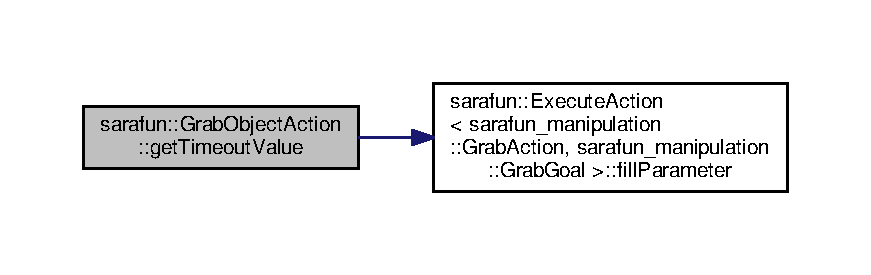
\includegraphics[width=350pt]{db/d0c/classsarafun_1_1GrabObjectAction_a6e2ee834fda8bd8d0dbdc101c8acdd9c_a6e2ee834fda8bd8d0dbdc101c8acdd9c_cgraph}
\end{center}
\end{figure}




\subsection{Field Documentation}
\hypertarget{classsarafun_1_1GrabObjectAction_a99b30dab79220943e417769f1a3d4f36_a99b30dab79220943e417769f1a3d4f36}{\index{sarafun\-::\-Grab\-Object\-Action@{sarafun\-::\-Grab\-Object\-Action}!bt\-\_\-name\-\_\-@{bt\-\_\-name\-\_\-}}
\index{bt\-\_\-name\-\_\-@{bt\-\_\-name\-\_\-}!sarafun::GrabObjectAction@{sarafun\-::\-Grab\-Object\-Action}}
\subsubsection[{bt\-\_\-name\-\_\-}]{\setlength{\rightskip}{0pt plus 5cm}std\-::string sarafun\-::\-Grab\-Object\-Action\-::bt\-\_\-name\-\_\-\hspace{0.3cm}{\ttfamily [private]}}}\label{classsarafun_1_1GrabObjectAction_a99b30dab79220943e417769f1a3d4f36_a99b30dab79220943e417769f1a3d4f36}


Definition at line 30 of file Grab\-Object\-Action.\-h.

\hypertarget{classsarafun_1_1GrabObjectAction_add955e0266ed5eaf3b6f7b3b3bccd4ae_add955e0266ed5eaf3b6f7b3b3bccd4ae}{\index{sarafun\-::\-Grab\-Object\-Action@{sarafun\-::\-Grab\-Object\-Action}!node\-\_\-handle\-\_\-@{node\-\_\-handle\-\_\-}}
\index{node\-\_\-handle\-\_\-@{node\-\_\-handle\-\_\-}!sarafun::GrabObjectAction@{sarafun\-::\-Grab\-Object\-Action}}
\subsubsection[{node\-\_\-handle\-\_\-}]{\setlength{\rightskip}{0pt plus 5cm}ros\-::\-Node\-Handle sarafun\-::\-Grab\-Object\-Action\-::node\-\_\-handle\-\_\-\hspace{0.3cm}{\ttfamily [private]}}}\label{classsarafun_1_1GrabObjectAction_add955e0266ed5eaf3b6f7b3b3bccd4ae_add955e0266ed5eaf3b6f7b3b3bccd4ae}


Definition at line 28 of file Grab\-Object\-Action.\-h.



Referenced by Grab\-Object\-Action().

\hypertarget{classsarafun_1_1GrabObjectAction_a586c34a94df1b7d435617d6b753d9e11_a586c34a94df1b7d435617d6b753d9e11}{\index{sarafun\-::\-Grab\-Object\-Action@{sarafun\-::\-Grab\-Object\-Action}!node\-\_\-name\-\_\-@{node\-\_\-name\-\_\-}}
\index{node\-\_\-name\-\_\-@{node\-\_\-name\-\_\-}!sarafun::GrabObjectAction@{sarafun\-::\-Grab\-Object\-Action}}
\subsubsection[{node\-\_\-name\-\_\-}]{\setlength{\rightskip}{0pt plus 5cm}std\-::string sarafun\-::\-Grab\-Object\-Action\-::node\-\_\-name\-\_\-\hspace{0.3cm}{\ttfamily [private]}}}\label{classsarafun_1_1GrabObjectAction_a586c34a94df1b7d435617d6b753d9e11_a586c34a94df1b7d435617d6b753d9e11}


Definition at line 29 of file Grab\-Object\-Action.\-h.



The documentation for this class was generated from the following files\-:\begin{DoxyCompactItemize}
\item 
Grab\-Object\-Action.\-h\item 
Grab\-Object\-Action.\-cpp\end{DoxyCompactItemize}

\hypertarget{classsarafun_1_1GraspAction}{\section{sarafun\-:\-:Grasp\-Action Class Reference}
\label{classsarafun_1_1GraspAction}\index{sarafun\-::\-Grasp\-Action@{sarafun\-::\-Grasp\-Action}}
}


{\ttfamily \#include $<$Grasp\-Action.\-h$>$}



Inheritance diagram for sarafun\-:\-:Grasp\-Action\-:\nopagebreak
\begin{figure}[H]
\begin{center}
\leavevmode
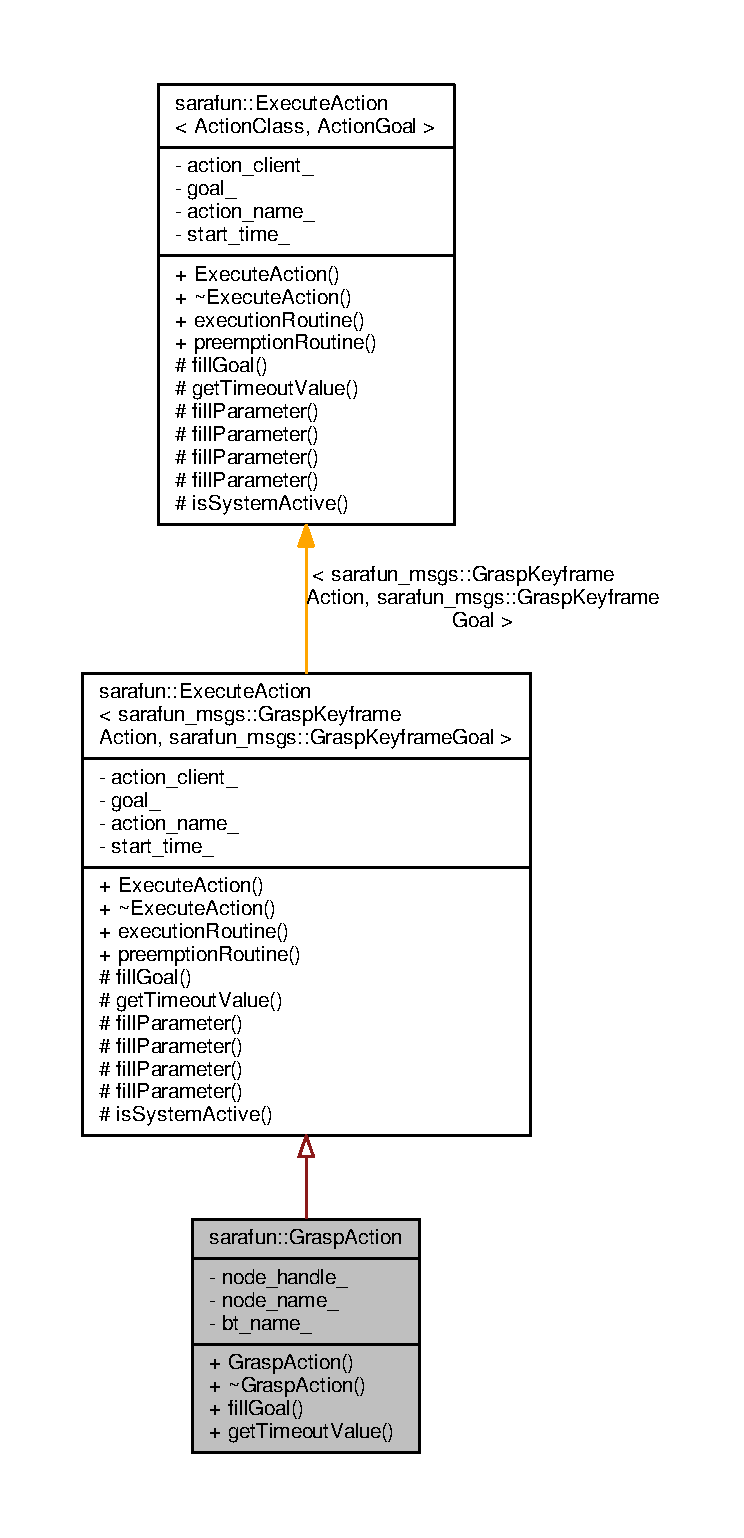
\includegraphics[height=550pt]{de/d55/classsarafun_1_1GraspAction__inherit__graph}
\end{center}
\end{figure}


Collaboration diagram for sarafun\-:\-:Grasp\-Action\-:\nopagebreak
\begin{figure}[H]
\begin{center}
\leavevmode
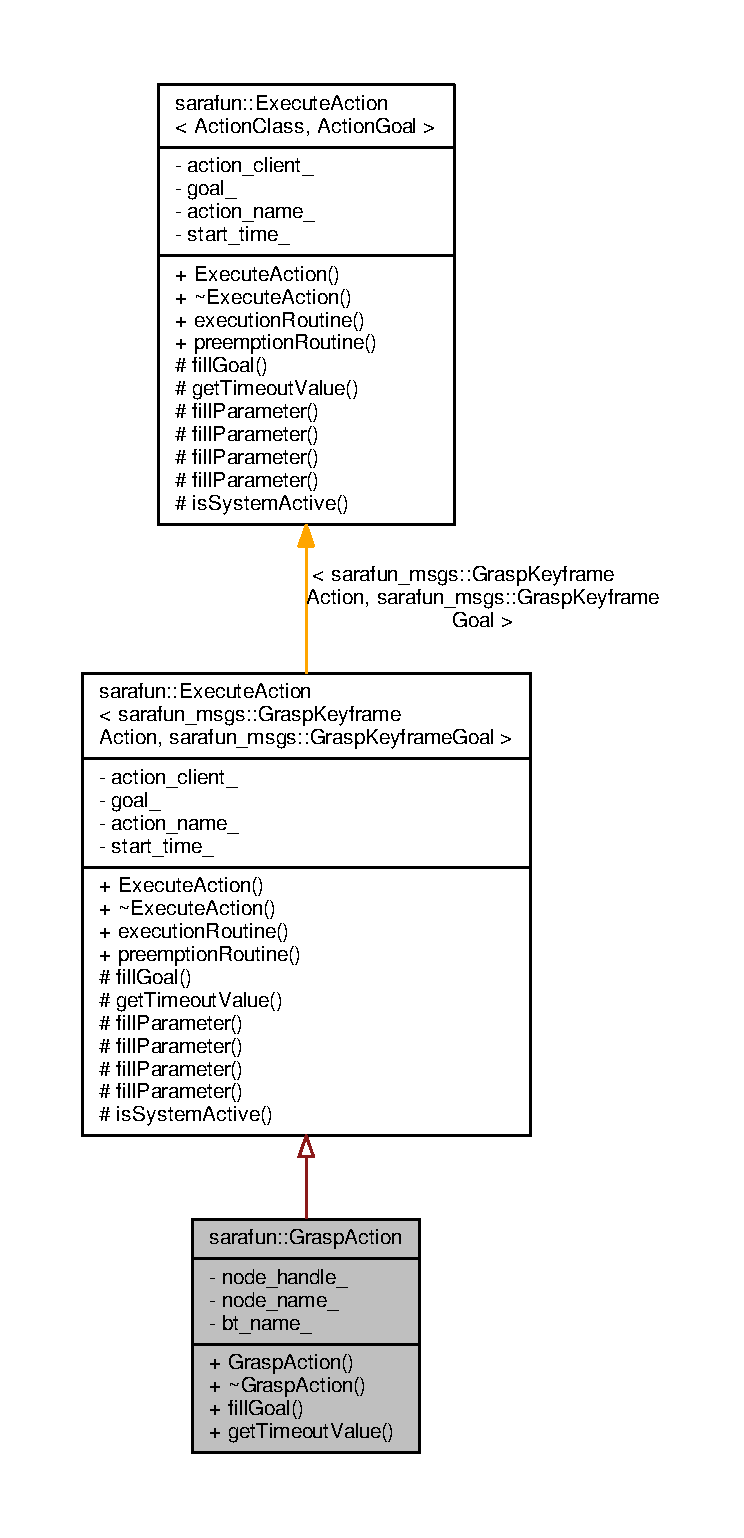
\includegraphics[height=550pt]{d0/dab/classsarafun_1_1GraspAction__coll__graph}
\end{center}
\end{figure}
\subsection*{Public Member Functions}
\begin{DoxyCompactItemize}
\item 
\hyperlink{classsarafun_1_1GraspAction_ae3eed6fe11388023bab8316803759ac5_ae3eed6fe11388023bab8316803759ac5}{Grasp\-Action} (std\-::string node\-\_\-name, std\-::string action\-\_\-name, std\-::string bt\-\_\-name)
\item 
\hyperlink{classsarafun_1_1GraspAction_aeb09ce6ab575e2653bfb88aa62b09361_aeb09ce6ab575e2653bfb88aa62b09361}{$\sim$\-Grasp\-Action} ()
\item 
bool \hyperlink{classsarafun_1_1GraspAction_a7418fe9de5024a8fbbfe8e5f5336d66f_a7418fe9de5024a8fbbfe8e5f5336d66f}{fill\-Goal} (sarafun\-\_\-msgs\-::\-Grasp\-Keyframe\-Goal \&goal)
\item 
double \hyperlink{classsarafun_1_1GraspAction_a406d5c86b5f788537c5af9d125724a55_a406d5c86b5f788537c5af9d125724a55}{get\-Timeout\-Value} ()
\end{DoxyCompactItemize}
\subsection*{Private Attributes}
\begin{DoxyCompactItemize}
\item 
ros\-::\-Node\-Handle \hyperlink{classsarafun_1_1GraspAction_a4b39e13eba27c71ee0d2cce0243b3e08_a4b39e13eba27c71ee0d2cce0243b3e08}{node\-\_\-handle\-\_\-}
\item 
std\-::string \hyperlink{classsarafun_1_1GraspAction_afd7e5985ad75e7b94ccd3190243d9df2_afd7e5985ad75e7b94ccd3190243d9df2}{node\-\_\-name\-\_\-}
\item 
std\-::string \hyperlink{classsarafun_1_1GraspAction_a3c06e926769370c2e80f864f8f36b958_a3c06e926769370c2e80f864f8f36b958}{bt\-\_\-name\-\_\-}
\end{DoxyCompactItemize}
\subsection*{Additional Inherited Members}


\subsection{Detailed Description}


Definition at line 9 of file Grasp\-Action.\-h.



\subsection{Constructor \& Destructor Documentation}
\hypertarget{classsarafun_1_1GraspAction_ae3eed6fe11388023bab8316803759ac5_ae3eed6fe11388023bab8316803759ac5}{\index{sarafun\-::\-Grasp\-Action@{sarafun\-::\-Grasp\-Action}!Grasp\-Action@{Grasp\-Action}}
\index{Grasp\-Action@{Grasp\-Action}!sarafun::GraspAction@{sarafun\-::\-Grasp\-Action}}
\subsubsection[{Grasp\-Action}]{\setlength{\rightskip}{0pt plus 5cm}sarafun\-::\-Grasp\-Action\-::\-Grasp\-Action (
\begin{DoxyParamCaption}
\item[{std\-::string}]{node\-\_\-name, }
\item[{std\-::string}]{action\-\_\-name, }
\item[{std\-::string}]{bt\-\_\-name}
\end{DoxyParamCaption}
)\hspace{0.3cm}{\ttfamily [inline]}}}\label{classsarafun_1_1GraspAction_ae3eed6fe11388023bab8316803759ac5_ae3eed6fe11388023bab8316803759ac5}


Definition at line 13 of file Grasp\-Action.\-h.



References node\-\_\-handle\-\_\-.

\hypertarget{classsarafun_1_1GraspAction_aeb09ce6ab575e2653bfb88aa62b09361_aeb09ce6ab575e2653bfb88aa62b09361}{\index{sarafun\-::\-Grasp\-Action@{sarafun\-::\-Grasp\-Action}!$\sim$\-Grasp\-Action@{$\sim$\-Grasp\-Action}}
\index{$\sim$\-Grasp\-Action@{$\sim$\-Grasp\-Action}!sarafun::GraspAction@{sarafun\-::\-Grasp\-Action}}
\subsubsection[{$\sim$\-Grasp\-Action}]{\setlength{\rightskip}{0pt plus 5cm}sarafun\-::\-Grasp\-Action\-::$\sim$\-Grasp\-Action (
\begin{DoxyParamCaption}
{}
\end{DoxyParamCaption}
)\hspace{0.3cm}{\ttfamily [inline]}}}\label{classsarafun_1_1GraspAction_aeb09ce6ab575e2653bfb88aa62b09361_aeb09ce6ab575e2653bfb88aa62b09361}


Definition at line 23 of file Grasp\-Action.\-h.



\subsection{Member Function Documentation}
\hypertarget{classsarafun_1_1GraspAction_a7418fe9de5024a8fbbfe8e5f5336d66f_a7418fe9de5024a8fbbfe8e5f5336d66f}{\index{sarafun\-::\-Grasp\-Action@{sarafun\-::\-Grasp\-Action}!fill\-Goal@{fill\-Goal}}
\index{fill\-Goal@{fill\-Goal}!sarafun::GraspAction@{sarafun\-::\-Grasp\-Action}}
\subsubsection[{fill\-Goal}]{\setlength{\rightskip}{0pt plus 5cm}bool sarafun\-::\-Grasp\-Action\-::fill\-Goal (
\begin{DoxyParamCaption}
\item[{sarafun\-\_\-msgs\-::\-Grasp\-Keyframe\-Goal \&}]{goal}
\end{DoxyParamCaption}
)\hspace{0.3cm}{\ttfamily [virtual]}}}\label{classsarafun_1_1GraspAction_a7418fe9de5024a8fbbfe8e5f5336d66f_a7418fe9de5024a8fbbfe8e5f5336d66f}
Fills in the goal for a particular action.


\begin{DoxyParams}{Parameters}
{\em goal} & The actionlib goal message of the externally implemented action. \\
\hline
\end{DoxyParams}
\begin{DoxyReturn}{Returns}
False in case of error, true otherwise. 
\end{DoxyReturn}


Implements \hyperlink{classsarafun_1_1ExecuteAction_a6dd9c0f013d15a17d7e7ce8dbe40a436_a6dd9c0f013d15a17d7e7ce8dbe40a436}{sarafun\-::\-Execute\-Action$<$ sarafun\-\_\-msgs\-::\-Grasp\-Keyframe\-Action, sarafun\-\_\-msgs\-::\-Grasp\-Keyframe\-Goal $>$}.



Definition at line 4 of file Grasp\-Action.\-cpp.

\hypertarget{classsarafun_1_1GraspAction_a406d5c86b5f788537c5af9d125724a55_a406d5c86b5f788537c5af9d125724a55}{\index{sarafun\-::\-Grasp\-Action@{sarafun\-::\-Grasp\-Action}!get\-Timeout\-Value@{get\-Timeout\-Value}}
\index{get\-Timeout\-Value@{get\-Timeout\-Value}!sarafun::GraspAction@{sarafun\-::\-Grasp\-Action}}
\subsubsection[{get\-Timeout\-Value}]{\setlength{\rightskip}{0pt plus 5cm}double sarafun\-::\-Grasp\-Action\-::get\-Timeout\-Value (
\begin{DoxyParamCaption}
{}
\end{DoxyParamCaption}
)\hspace{0.3cm}{\ttfamily [virtual]}}}\label{classsarafun_1_1GraspAction_a406d5c86b5f788537c5af9d125724a55_a406d5c86b5f788537c5af9d125724a55}
Provides the client with a timeout value for actionlib connections.

\begin{DoxyReturn}{Returns}
The timeout value (in seconds). 
\end{DoxyReturn}


Implements \hyperlink{classsarafun_1_1ExecuteAction_aba6cfa8a8ce19e735eb6394424df6d17_aba6cfa8a8ce19e735eb6394424df6d17}{sarafun\-::\-Execute\-Action$<$ sarafun\-\_\-msgs\-::\-Grasp\-Keyframe\-Action, sarafun\-\_\-msgs\-::\-Grasp\-Keyframe\-Goal $>$}.



Definition at line 8 of file Grasp\-Action.\-cpp.



References sarafun\-::\-Execute\-Action$<$ sarafun\-\_\-msgs\-::\-Grasp\-Keyframe\-Action, sarafun\-\_\-msgs\-::\-Grasp\-Keyframe\-Goal $>$\-::fill\-Parameter().



Here is the call graph for this function\-:\nopagebreak
\begin{figure}[H]
\begin{center}
\leavevmode
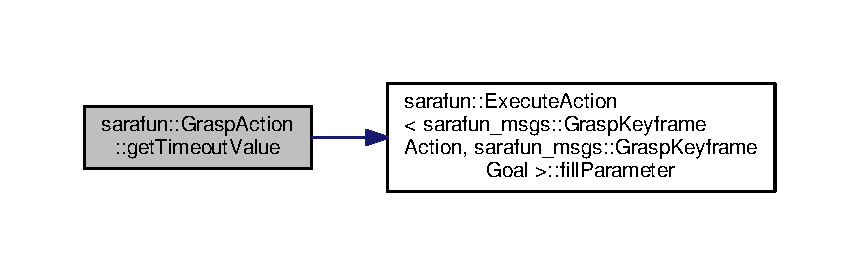
\includegraphics[width=350pt]{d0/d03/classsarafun_1_1GraspAction_a406d5c86b5f788537c5af9d125724a55_a406d5c86b5f788537c5af9d125724a55_cgraph}
\end{center}
\end{figure}




\subsection{Field Documentation}
\hypertarget{classsarafun_1_1GraspAction_a3c06e926769370c2e80f864f8f36b958_a3c06e926769370c2e80f864f8f36b958}{\index{sarafun\-::\-Grasp\-Action@{sarafun\-::\-Grasp\-Action}!bt\-\_\-name\-\_\-@{bt\-\_\-name\-\_\-}}
\index{bt\-\_\-name\-\_\-@{bt\-\_\-name\-\_\-}!sarafun::GraspAction@{sarafun\-::\-Grasp\-Action}}
\subsubsection[{bt\-\_\-name\-\_\-}]{\setlength{\rightskip}{0pt plus 5cm}std\-::string sarafun\-::\-Grasp\-Action\-::bt\-\_\-name\-\_\-\hspace{0.3cm}{\ttfamily [private]}}}\label{classsarafun_1_1GraspAction_a3c06e926769370c2e80f864f8f36b958_a3c06e926769370c2e80f864f8f36b958}


Definition at line 31 of file Grasp\-Action.\-h.

\hypertarget{classsarafun_1_1GraspAction_a4b39e13eba27c71ee0d2cce0243b3e08_a4b39e13eba27c71ee0d2cce0243b3e08}{\index{sarafun\-::\-Grasp\-Action@{sarafun\-::\-Grasp\-Action}!node\-\_\-handle\-\_\-@{node\-\_\-handle\-\_\-}}
\index{node\-\_\-handle\-\_\-@{node\-\_\-handle\-\_\-}!sarafun::GraspAction@{sarafun\-::\-Grasp\-Action}}
\subsubsection[{node\-\_\-handle\-\_\-}]{\setlength{\rightskip}{0pt plus 5cm}ros\-::\-Node\-Handle sarafun\-::\-Grasp\-Action\-::node\-\_\-handle\-\_\-\hspace{0.3cm}{\ttfamily [private]}}}\label{classsarafun_1_1GraspAction_a4b39e13eba27c71ee0d2cce0243b3e08_a4b39e13eba27c71ee0d2cce0243b3e08}


Definition at line 29 of file Grasp\-Action.\-h.



Referenced by Grasp\-Action().

\hypertarget{classsarafun_1_1GraspAction_afd7e5985ad75e7b94ccd3190243d9df2_afd7e5985ad75e7b94ccd3190243d9df2}{\index{sarafun\-::\-Grasp\-Action@{sarafun\-::\-Grasp\-Action}!node\-\_\-name\-\_\-@{node\-\_\-name\-\_\-}}
\index{node\-\_\-name\-\_\-@{node\-\_\-name\-\_\-}!sarafun::GraspAction@{sarafun\-::\-Grasp\-Action}}
\subsubsection[{node\-\_\-name\-\_\-}]{\setlength{\rightskip}{0pt plus 5cm}std\-::string sarafun\-::\-Grasp\-Action\-::node\-\_\-name\-\_\-\hspace{0.3cm}{\ttfamily [private]}}}\label{classsarafun_1_1GraspAction_afd7e5985ad75e7b94ccd3190243d9df2_afd7e5985ad75e7b94ccd3190243d9df2}


Definition at line 30 of file Grasp\-Action.\-h.



The documentation for this class was generated from the following files\-:\begin{DoxyCompactItemize}
\item 
Grasp\-Action.\-h\item 
Grasp\-Action.\-cpp\end{DoxyCompactItemize}

\hypertarget{classsarafun_1_1InitialAction}{\section{sarafun\-:\-:Initial\-Action Class Reference}
\label{classsarafun_1_1InitialAction}\index{sarafun\-::\-Initial\-Action@{sarafun\-::\-Initial\-Action}}
}


{\ttfamily \#include $<$Initial\-Action.\-h$>$}



Inheritance diagram for sarafun\-:\-:Initial\-Action\-:\nopagebreak
\begin{figure}[H]
\begin{center}
\leavevmode
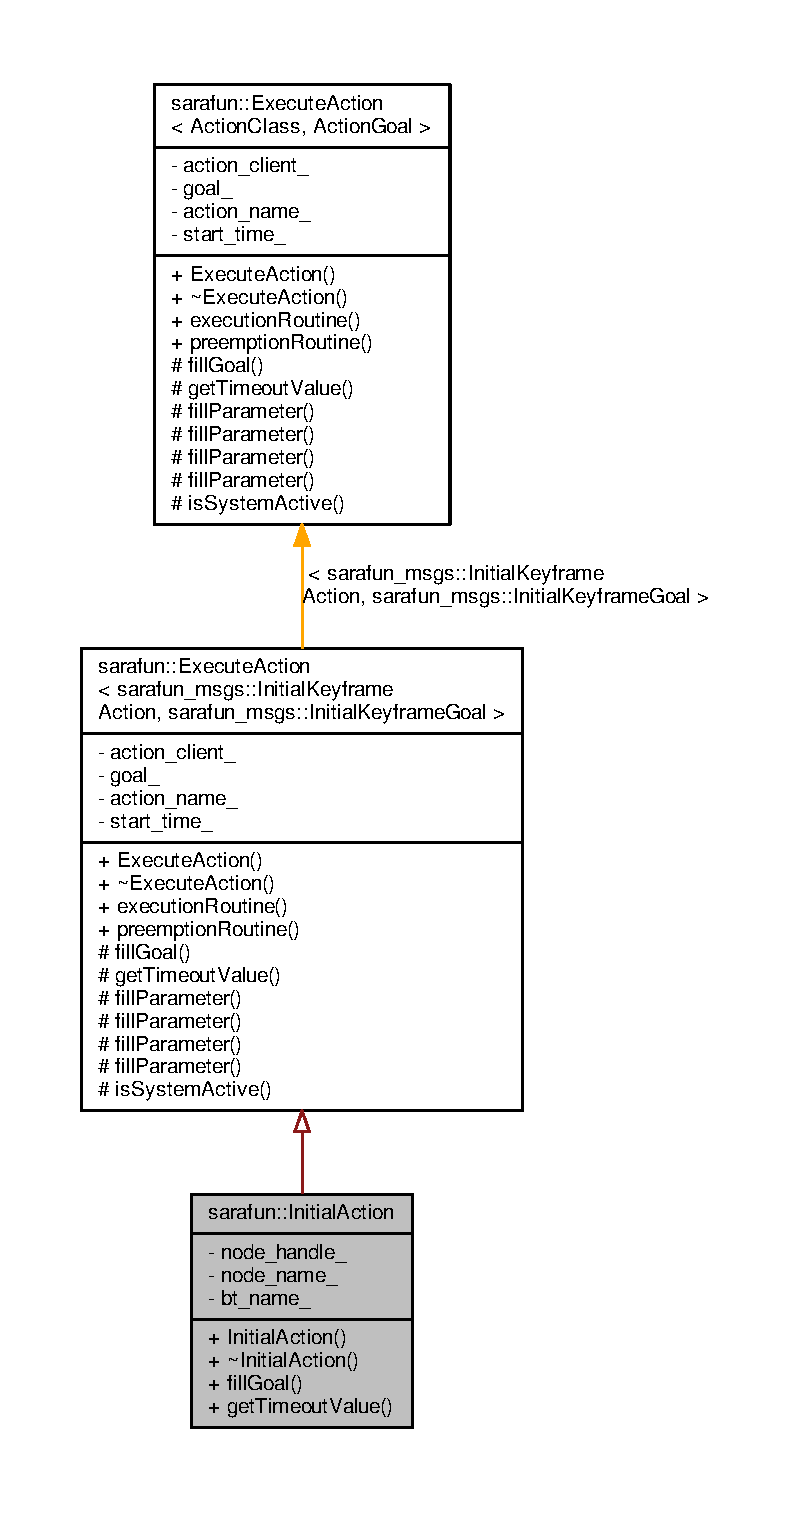
\includegraphics[height=550pt]{d2/dd7/classsarafun_1_1InitialAction__inherit__graph}
\end{center}
\end{figure}


Collaboration diagram for sarafun\-:\-:Initial\-Action\-:\nopagebreak
\begin{figure}[H]
\begin{center}
\leavevmode
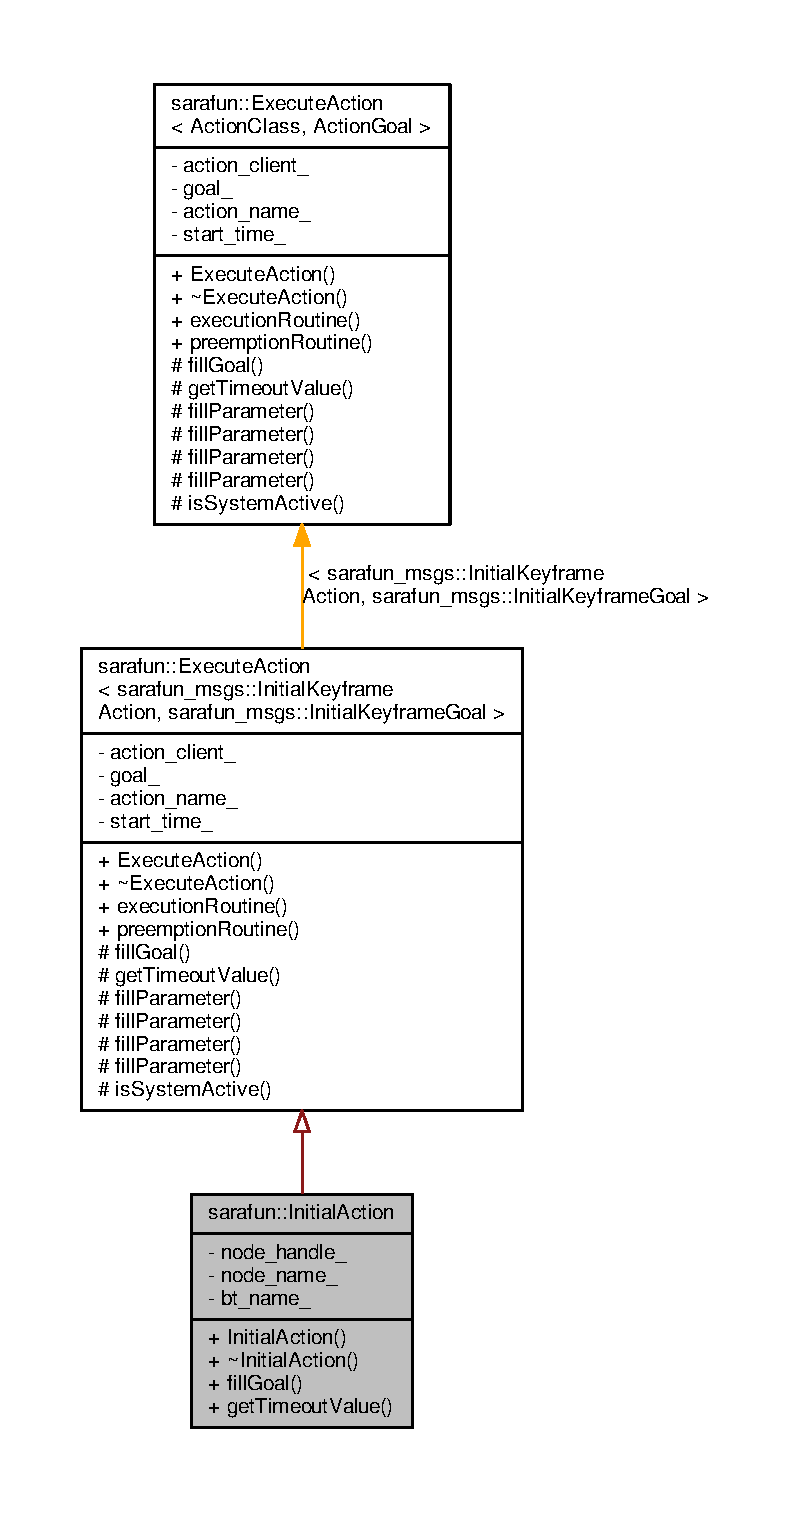
\includegraphics[height=550pt]{da/d64/classsarafun_1_1InitialAction__coll__graph}
\end{center}
\end{figure}
\subsection*{Public Member Functions}
\begin{DoxyCompactItemize}
\item 
\hyperlink{classsarafun_1_1InitialAction_afecd855fe18671ea36bdab881603e8bc_afecd855fe18671ea36bdab881603e8bc}{Initial\-Action} (std\-::string node\-\_\-name, std\-::string action\-\_\-name, std\-::string bt\-\_\-name)
\item 
\hyperlink{classsarafun_1_1InitialAction_af1f0a71513d093f5c2d7657b4b84661b_af1f0a71513d093f5c2d7657b4b84661b}{$\sim$\-Initial\-Action} ()
\item 
bool \hyperlink{classsarafun_1_1InitialAction_aac7f439c30455349e075e91542565a43_aac7f439c30455349e075e91542565a43}{fill\-Goal} (sarafun\-\_\-msgs\-::\-Initial\-Keyframe\-Goal \&goal)
\item 
double \hyperlink{classsarafun_1_1InitialAction_a1b58c06c32ec9f9d3e75c37de5e7d2c8_a1b58c06c32ec9f9d3e75c37de5e7d2c8}{get\-Timeout\-Value} ()
\end{DoxyCompactItemize}
\subsection*{Private Attributes}
\begin{DoxyCompactItemize}
\item 
ros\-::\-Node\-Handle \hyperlink{classsarafun_1_1InitialAction_ab28f63a6c2bfb376d0c52b619fb6b473_ab28f63a6c2bfb376d0c52b619fb6b473}{node\-\_\-handle\-\_\-}
\item 
std\-::string \hyperlink{classsarafun_1_1InitialAction_a985fe910cf04f8e6f918672175eb8ca6_a985fe910cf04f8e6f918672175eb8ca6}{node\-\_\-name\-\_\-}
\item 
std\-::string \hyperlink{classsarafun_1_1InitialAction_aaa1d120b5ff08ffaebe777d8f3793be3_aaa1d120b5ff08ffaebe777d8f3793be3}{bt\-\_\-name\-\_\-}
\end{DoxyCompactItemize}
\subsection*{Additional Inherited Members}


\subsection{Detailed Description}


Definition at line 9 of file Initial\-Action.\-h.



\subsection{Constructor \& Destructor Documentation}
\hypertarget{classsarafun_1_1InitialAction_afecd855fe18671ea36bdab881603e8bc_afecd855fe18671ea36bdab881603e8bc}{\index{sarafun\-::\-Initial\-Action@{sarafun\-::\-Initial\-Action}!Initial\-Action@{Initial\-Action}}
\index{Initial\-Action@{Initial\-Action}!sarafun::InitialAction@{sarafun\-::\-Initial\-Action}}
\subsubsection[{Initial\-Action}]{\setlength{\rightskip}{0pt plus 5cm}sarafun\-::\-Initial\-Action\-::\-Initial\-Action (
\begin{DoxyParamCaption}
\item[{std\-::string}]{node\-\_\-name, }
\item[{std\-::string}]{action\-\_\-name, }
\item[{std\-::string}]{bt\-\_\-name}
\end{DoxyParamCaption}
)\hspace{0.3cm}{\ttfamily [inline]}}}\label{classsarafun_1_1InitialAction_afecd855fe18671ea36bdab881603e8bc_afecd855fe18671ea36bdab881603e8bc}


Definition at line 13 of file Initial\-Action.\-h.



References node\-\_\-handle\-\_\-.

\hypertarget{classsarafun_1_1InitialAction_af1f0a71513d093f5c2d7657b4b84661b_af1f0a71513d093f5c2d7657b4b84661b}{\index{sarafun\-::\-Initial\-Action@{sarafun\-::\-Initial\-Action}!$\sim$\-Initial\-Action@{$\sim$\-Initial\-Action}}
\index{$\sim$\-Initial\-Action@{$\sim$\-Initial\-Action}!sarafun::InitialAction@{sarafun\-::\-Initial\-Action}}
\subsubsection[{$\sim$\-Initial\-Action}]{\setlength{\rightskip}{0pt plus 5cm}sarafun\-::\-Initial\-Action\-::$\sim$\-Initial\-Action (
\begin{DoxyParamCaption}
{}
\end{DoxyParamCaption}
)\hspace{0.3cm}{\ttfamily [inline]}}}\label{classsarafun_1_1InitialAction_af1f0a71513d093f5c2d7657b4b84661b_af1f0a71513d093f5c2d7657b4b84661b}


Definition at line 23 of file Initial\-Action.\-h.



\subsection{Member Function Documentation}
\hypertarget{classsarafun_1_1InitialAction_aac7f439c30455349e075e91542565a43_aac7f439c30455349e075e91542565a43}{\index{sarafun\-::\-Initial\-Action@{sarafun\-::\-Initial\-Action}!fill\-Goal@{fill\-Goal}}
\index{fill\-Goal@{fill\-Goal}!sarafun::InitialAction@{sarafun\-::\-Initial\-Action}}
\subsubsection[{fill\-Goal}]{\setlength{\rightskip}{0pt plus 5cm}bool sarafun\-::\-Initial\-Action\-::fill\-Goal (
\begin{DoxyParamCaption}
\item[{sarafun\-\_\-msgs\-::\-Initial\-Keyframe\-Goal \&}]{goal}
\end{DoxyParamCaption}
)\hspace{0.3cm}{\ttfamily [virtual]}}}\label{classsarafun_1_1InitialAction_aac7f439c30455349e075e91542565a43_aac7f439c30455349e075e91542565a43}
Fills in the goal for a particular action.


\begin{DoxyParams}{Parameters}
{\em goal} & The actionlib goal message of the externally implemented action. \\
\hline
\end{DoxyParams}
\begin{DoxyReturn}{Returns}
False in case of error, true otherwise. 
\end{DoxyReturn}


Implements \hyperlink{classsarafun_1_1ExecuteAction_a6dd9c0f013d15a17d7e7ce8dbe40a436_a6dd9c0f013d15a17d7e7ce8dbe40a436}{sarafun\-::\-Execute\-Action$<$ sarafun\-\_\-msgs\-::\-Initial\-Keyframe\-Action, sarafun\-\_\-msgs\-::\-Initial\-Keyframe\-Goal $>$}.



Definition at line 4 of file Initial\-Action.\-cpp.



References sarafun\-::\-Execute\-Action$<$ sarafun\-\_\-msgs\-::\-Initial\-Keyframe\-Action, sarafun\-\_\-msgs\-::\-Initial\-Keyframe\-Goal $>$\-::fill\-Parameter().



Here is the call graph for this function\-:\nopagebreak
\begin{figure}[H]
\begin{center}
\leavevmode
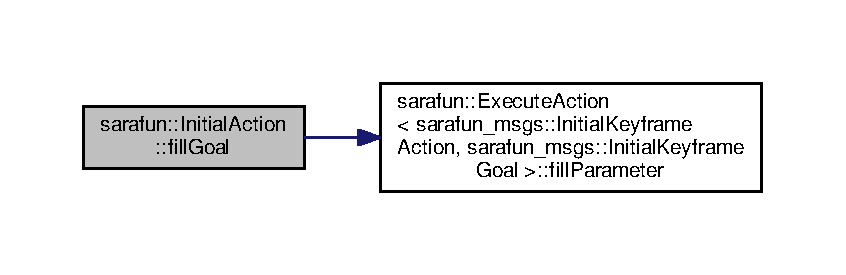
\includegraphics[width=350pt]{d6/d64/classsarafun_1_1InitialAction_aac7f439c30455349e075e91542565a43_aac7f439c30455349e075e91542565a43_cgraph}
\end{center}
\end{figure}


\hypertarget{classsarafun_1_1InitialAction_a1b58c06c32ec9f9d3e75c37de5e7d2c8_a1b58c06c32ec9f9d3e75c37de5e7d2c8}{\index{sarafun\-::\-Initial\-Action@{sarafun\-::\-Initial\-Action}!get\-Timeout\-Value@{get\-Timeout\-Value}}
\index{get\-Timeout\-Value@{get\-Timeout\-Value}!sarafun::InitialAction@{sarafun\-::\-Initial\-Action}}
\subsubsection[{get\-Timeout\-Value}]{\setlength{\rightskip}{0pt plus 5cm}double sarafun\-::\-Initial\-Action\-::get\-Timeout\-Value (
\begin{DoxyParamCaption}
{}
\end{DoxyParamCaption}
)\hspace{0.3cm}{\ttfamily [virtual]}}}\label{classsarafun_1_1InitialAction_a1b58c06c32ec9f9d3e75c37de5e7d2c8_a1b58c06c32ec9f9d3e75c37de5e7d2c8}
Provides the client with a timeout value for actionlib connections.

\begin{DoxyReturn}{Returns}
The timeout value (in seconds). 
\end{DoxyReturn}


Implements \hyperlink{classsarafun_1_1ExecuteAction_aba6cfa8a8ce19e735eb6394424df6d17_aba6cfa8a8ce19e735eb6394424df6d17}{sarafun\-::\-Execute\-Action$<$ sarafun\-\_\-msgs\-::\-Initial\-Keyframe\-Action, sarafun\-\_\-msgs\-::\-Initial\-Keyframe\-Goal $>$}.



Definition at line 13 of file Initial\-Action.\-cpp.



References sarafun\-::\-Execute\-Action$<$ sarafun\-\_\-msgs\-::\-Initial\-Keyframe\-Action, sarafun\-\_\-msgs\-::\-Initial\-Keyframe\-Goal $>$\-::fill\-Parameter().



Here is the call graph for this function\-:\nopagebreak
\begin{figure}[H]
\begin{center}
\leavevmode
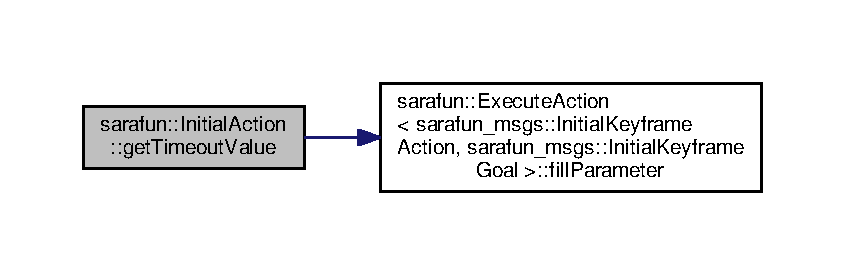
\includegraphics[width=350pt]{d6/d64/classsarafun_1_1InitialAction_a1b58c06c32ec9f9d3e75c37de5e7d2c8_a1b58c06c32ec9f9d3e75c37de5e7d2c8_cgraph}
\end{center}
\end{figure}




\subsection{Field Documentation}
\hypertarget{classsarafun_1_1InitialAction_aaa1d120b5ff08ffaebe777d8f3793be3_aaa1d120b5ff08ffaebe777d8f3793be3}{\index{sarafun\-::\-Initial\-Action@{sarafun\-::\-Initial\-Action}!bt\-\_\-name\-\_\-@{bt\-\_\-name\-\_\-}}
\index{bt\-\_\-name\-\_\-@{bt\-\_\-name\-\_\-}!sarafun::InitialAction@{sarafun\-::\-Initial\-Action}}
\subsubsection[{bt\-\_\-name\-\_\-}]{\setlength{\rightskip}{0pt plus 5cm}std\-::string sarafun\-::\-Initial\-Action\-::bt\-\_\-name\-\_\-\hspace{0.3cm}{\ttfamily [private]}}}\label{classsarafun_1_1InitialAction_aaa1d120b5ff08ffaebe777d8f3793be3_aaa1d120b5ff08ffaebe777d8f3793be3}


Definition at line 31 of file Initial\-Action.\-h.

\hypertarget{classsarafun_1_1InitialAction_ab28f63a6c2bfb376d0c52b619fb6b473_ab28f63a6c2bfb376d0c52b619fb6b473}{\index{sarafun\-::\-Initial\-Action@{sarafun\-::\-Initial\-Action}!node\-\_\-handle\-\_\-@{node\-\_\-handle\-\_\-}}
\index{node\-\_\-handle\-\_\-@{node\-\_\-handle\-\_\-}!sarafun::InitialAction@{sarafun\-::\-Initial\-Action}}
\subsubsection[{node\-\_\-handle\-\_\-}]{\setlength{\rightskip}{0pt plus 5cm}ros\-::\-Node\-Handle sarafun\-::\-Initial\-Action\-::node\-\_\-handle\-\_\-\hspace{0.3cm}{\ttfamily [private]}}}\label{classsarafun_1_1InitialAction_ab28f63a6c2bfb376d0c52b619fb6b473_ab28f63a6c2bfb376d0c52b619fb6b473}


Definition at line 29 of file Initial\-Action.\-h.



Referenced by Initial\-Action().

\hypertarget{classsarafun_1_1InitialAction_a985fe910cf04f8e6f918672175eb8ca6_a985fe910cf04f8e6f918672175eb8ca6}{\index{sarafun\-::\-Initial\-Action@{sarafun\-::\-Initial\-Action}!node\-\_\-name\-\_\-@{node\-\_\-name\-\_\-}}
\index{node\-\_\-name\-\_\-@{node\-\_\-name\-\_\-}!sarafun::InitialAction@{sarafun\-::\-Initial\-Action}}
\subsubsection[{node\-\_\-name\-\_\-}]{\setlength{\rightskip}{0pt plus 5cm}std\-::string sarafun\-::\-Initial\-Action\-::node\-\_\-name\-\_\-\hspace{0.3cm}{\ttfamily [private]}}}\label{classsarafun_1_1InitialAction_a985fe910cf04f8e6f918672175eb8ca6_a985fe910cf04f8e6f918672175eb8ca6}


Definition at line 30 of file Initial\-Action.\-h.



The documentation for this class was generated from the following files\-:\begin{DoxyCompactItemize}
\item 
Initial\-Action.\-h\item 
Initial\-Action.\-cpp\end{DoxyCompactItemize}

\hypertarget{classsarafun_1_1InsertionWithDeformationAction}{\section{sarafun\-:\-:Insertion\-With\-Deformation\-Action Class Reference}
\label{classsarafun_1_1InsertionWithDeformationAction}\index{sarafun\-::\-Insertion\-With\-Deformation\-Action@{sarafun\-::\-Insertion\-With\-Deformation\-Action}}
}


{\ttfamily \#include $<$Insertion\-With\-Deformation\-Action.\-h$>$}



Inheritance diagram for sarafun\-:\-:Insertion\-With\-Deformation\-Action\-:
\nopagebreak
\begin{figure}[H]
\begin{center}
\leavevmode
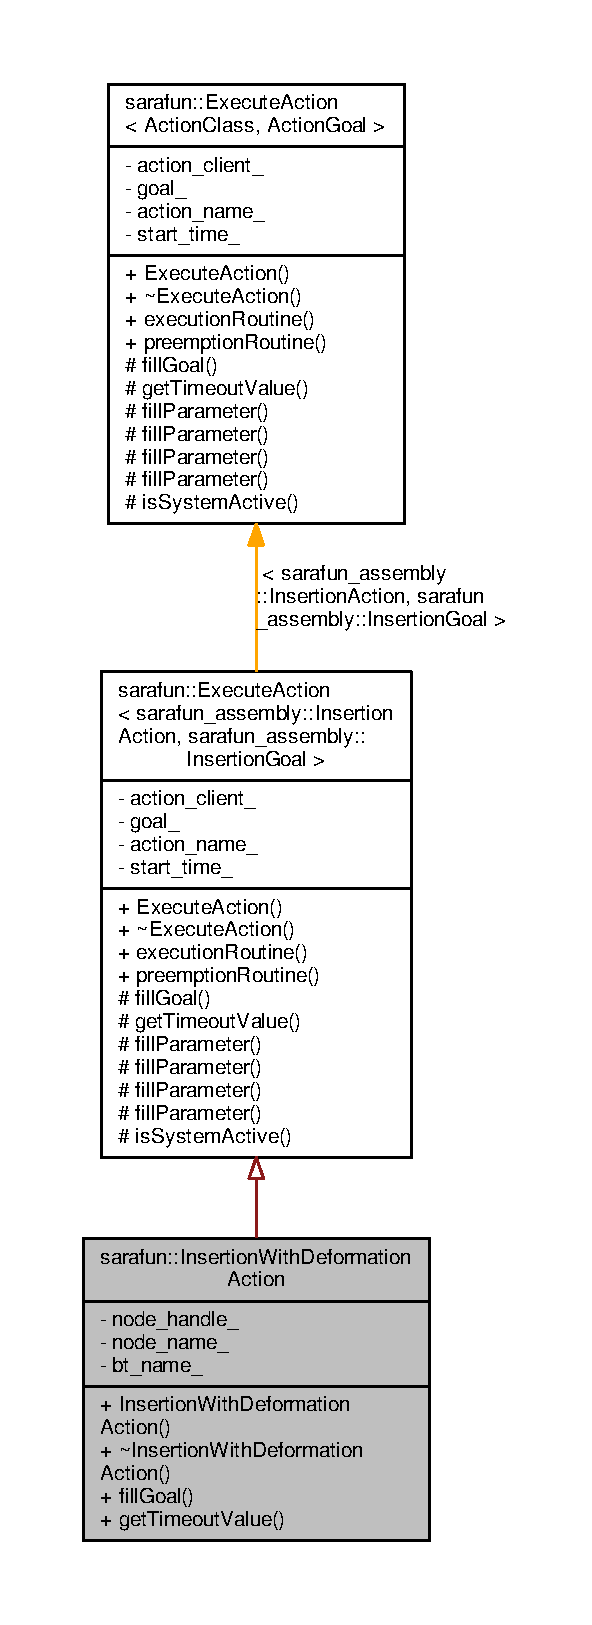
\includegraphics[height=550pt]{de/dd8/classsarafun_1_1InsertionWithDeformationAction__inherit__graph}
\end{center}
\end{figure}


Collaboration diagram for sarafun\-:\-:Insertion\-With\-Deformation\-Action\-:
\nopagebreak
\begin{figure}[H]
\begin{center}
\leavevmode
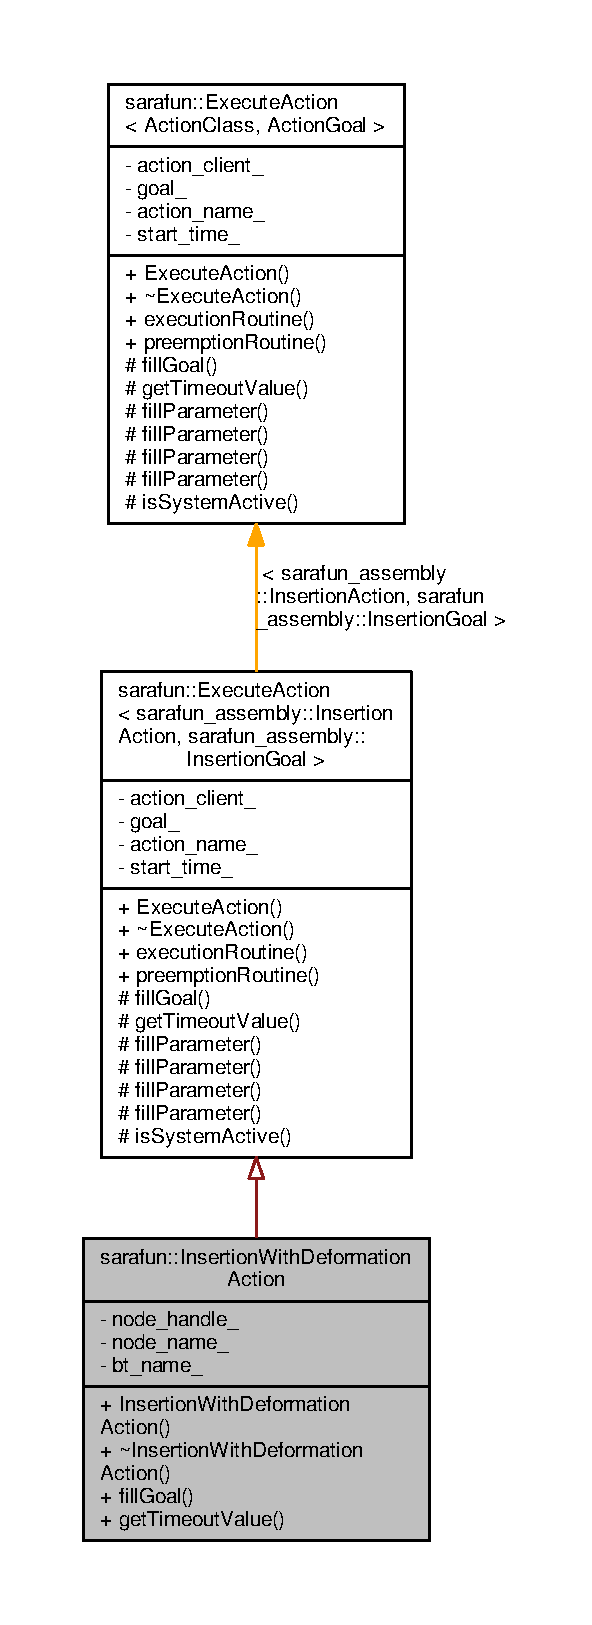
\includegraphics[height=550pt]{da/dd6/classsarafun_1_1InsertionWithDeformationAction__coll__graph}
\end{center}
\end{figure}
\subsection*{Public Member Functions}
\begin{DoxyCompactItemize}
\item 
\hyperlink{classsarafun_1_1InsertionWithDeformationAction_a2b851f2604c6a10f32b1d4b51bfae6a8_a2b851f2604c6a10f32b1d4b51bfae6a8}{Insertion\-With\-Deformation\-Action} (std\-::string node\-\_\-name, std\-::string action\-\_\-name, std\-::string bt\-\_\-name)
\item 
\hyperlink{classsarafun_1_1InsertionWithDeformationAction_a9b8740951e51538bf47d6534b8b4fe36_a9b8740951e51538bf47d6534b8b4fe36}{$\sim$\-Insertion\-With\-Deformation\-Action} ()
\item 
bool \hyperlink{classsarafun_1_1InsertionWithDeformationAction_a32d695dfcd626c5a7ca0fa987c245083_a32d695dfcd626c5a7ca0fa987c245083}{fill\-Goal} (sarafun\-\_\-assembly\-::\-Insertion\-Goal \&goal)
\item 
double \hyperlink{classsarafun_1_1InsertionWithDeformationAction_a8d77b104fb2396000b273cb6754ff879_a8d77b104fb2396000b273cb6754ff879}{get\-Timeout\-Value} ()
\end{DoxyCompactItemize}
\subsection*{Private Attributes}
\begin{DoxyCompactItemize}
\item 
ros\-::\-Node\-Handle \hyperlink{classsarafun_1_1InsertionWithDeformationAction_a97fcbe6b19d7f2185e19f5e8397b2307_a97fcbe6b19d7f2185e19f5e8397b2307}{node\-\_\-handle\-\_\-}
\item 
std\-::string \hyperlink{classsarafun_1_1InsertionWithDeformationAction_a493a532429347d18fa4d525d982c0204_a493a532429347d18fa4d525d982c0204}{node\-\_\-name\-\_\-}
\item 
std\-::string \hyperlink{classsarafun_1_1InsertionWithDeformationAction_aa5a6397046e4d8ac145d2961d04fc27c_aa5a6397046e4d8ac145d2961d04fc27c}{bt\-\_\-name\-\_\-}
\end{DoxyCompactItemize}
\subsection*{Additional Inherited Members}


\subsection{Detailed Description}


Definition at line 9 of file Insertion\-With\-Deformation\-Action.\-h.



\subsection{Constructor \& Destructor Documentation}
\hypertarget{classsarafun_1_1InsertionWithDeformationAction_a2b851f2604c6a10f32b1d4b51bfae6a8_a2b851f2604c6a10f32b1d4b51bfae6a8}{\index{sarafun\-::\-Insertion\-With\-Deformation\-Action@{sarafun\-::\-Insertion\-With\-Deformation\-Action}!Insertion\-With\-Deformation\-Action@{Insertion\-With\-Deformation\-Action}}
\index{Insertion\-With\-Deformation\-Action@{Insertion\-With\-Deformation\-Action}!sarafun::InsertionWithDeformationAction@{sarafun\-::\-Insertion\-With\-Deformation\-Action}}
\subsubsection[{Insertion\-With\-Deformation\-Action}]{\setlength{\rightskip}{0pt plus 5cm}sarafun\-::\-Insertion\-With\-Deformation\-Action\-::\-Insertion\-With\-Deformation\-Action (
\begin{DoxyParamCaption}
\item[{std\-::string}]{node\-\_\-name, }
\item[{std\-::string}]{action\-\_\-name, }
\item[{std\-::string}]{bt\-\_\-name}
\end{DoxyParamCaption}
)\hspace{0.3cm}{\ttfamily [inline]}}}\label{classsarafun_1_1InsertionWithDeformationAction_a2b851f2604c6a10f32b1d4b51bfae6a8_a2b851f2604c6a10f32b1d4b51bfae6a8}


Definition at line 13 of file Insertion\-With\-Deformation\-Action.\-h.



References node\-\_\-handle\-\_\-.

\hypertarget{classsarafun_1_1InsertionWithDeformationAction_a9b8740951e51538bf47d6534b8b4fe36_a9b8740951e51538bf47d6534b8b4fe36}{\index{sarafun\-::\-Insertion\-With\-Deformation\-Action@{sarafun\-::\-Insertion\-With\-Deformation\-Action}!$\sim$\-Insertion\-With\-Deformation\-Action@{$\sim$\-Insertion\-With\-Deformation\-Action}}
\index{$\sim$\-Insertion\-With\-Deformation\-Action@{$\sim$\-Insertion\-With\-Deformation\-Action}!sarafun::InsertionWithDeformationAction@{sarafun\-::\-Insertion\-With\-Deformation\-Action}}
\subsubsection[{$\sim$\-Insertion\-With\-Deformation\-Action}]{\setlength{\rightskip}{0pt plus 5cm}sarafun\-::\-Insertion\-With\-Deformation\-Action\-::$\sim$\-Insertion\-With\-Deformation\-Action (
\begin{DoxyParamCaption}
{}
\end{DoxyParamCaption}
)\hspace{0.3cm}{\ttfamily [inline]}}}\label{classsarafun_1_1InsertionWithDeformationAction_a9b8740951e51538bf47d6534b8b4fe36_a9b8740951e51538bf47d6534b8b4fe36}


Definition at line 23 of file Insertion\-With\-Deformation\-Action.\-h.



\subsection{Member Function Documentation}
\hypertarget{classsarafun_1_1InsertionWithDeformationAction_a32d695dfcd626c5a7ca0fa987c245083_a32d695dfcd626c5a7ca0fa987c245083}{\index{sarafun\-::\-Insertion\-With\-Deformation\-Action@{sarafun\-::\-Insertion\-With\-Deformation\-Action}!fill\-Goal@{fill\-Goal}}
\index{fill\-Goal@{fill\-Goal}!sarafun::InsertionWithDeformationAction@{sarafun\-::\-Insertion\-With\-Deformation\-Action}}
\subsubsection[{fill\-Goal}]{\setlength{\rightskip}{0pt plus 5cm}bool sarafun\-::\-Insertion\-With\-Deformation\-Action\-::fill\-Goal (
\begin{DoxyParamCaption}
\item[{sarafun\-\_\-assembly\-::\-Insertion\-Goal \&}]{goal}
\end{DoxyParamCaption}
)\hspace{0.3cm}{\ttfamily [virtual]}}}\label{classsarafun_1_1InsertionWithDeformationAction_a32d695dfcd626c5a7ca0fa987c245083_a32d695dfcd626c5a7ca0fa987c245083}
Fills in the goal for a particular action.


\begin{DoxyParams}{Parameters}
{\em goal} & The actionlib goal message of the externally implemented action. \\
\hline
\end{DoxyParams}
\begin{DoxyReturn}{Returns}
False in case of error, true otherwise. 
\end{DoxyReturn}


Implements \hyperlink{classsarafun_1_1ExecuteAction_a6dd9c0f013d15a17d7e7ce8dbe40a436_a6dd9c0f013d15a17d7e7ce8dbe40a436}{sarafun\-::\-Execute\-Action$<$ sarafun\-\_\-assembly\-::\-Insertion\-Action, sarafun\-\_\-assembly\-::\-Insertion\-Goal $>$}.



Definition at line 11 of file Insertion\-With\-Deformation\-Action.\-cpp.

\hypertarget{classsarafun_1_1InsertionWithDeformationAction_a8d77b104fb2396000b273cb6754ff879_a8d77b104fb2396000b273cb6754ff879}{\index{sarafun\-::\-Insertion\-With\-Deformation\-Action@{sarafun\-::\-Insertion\-With\-Deformation\-Action}!get\-Timeout\-Value@{get\-Timeout\-Value}}
\index{get\-Timeout\-Value@{get\-Timeout\-Value}!sarafun::InsertionWithDeformationAction@{sarafun\-::\-Insertion\-With\-Deformation\-Action}}
\subsubsection[{get\-Timeout\-Value}]{\setlength{\rightskip}{0pt plus 5cm}double sarafun\-::\-Insertion\-With\-Deformation\-Action\-::get\-Timeout\-Value (
\begin{DoxyParamCaption}
{}
\end{DoxyParamCaption}
)\hspace{0.3cm}{\ttfamily [virtual]}}}\label{classsarafun_1_1InsertionWithDeformationAction_a8d77b104fb2396000b273cb6754ff879_a8d77b104fb2396000b273cb6754ff879}
Provides the client with a timeout value for actionlib connections.

\begin{DoxyReturn}{Returns}
The timeout value (in seconds). 
\end{DoxyReturn}


Implements \hyperlink{classsarafun_1_1ExecuteAction_aba6cfa8a8ce19e735eb6394424df6d17_aba6cfa8a8ce19e735eb6394424df6d17}{sarafun\-::\-Execute\-Action$<$ sarafun\-\_\-assembly\-::\-Insertion\-Action, sarafun\-\_\-assembly\-::\-Insertion\-Goal $>$}.



Definition at line 4 of file Insertion\-With\-Deformation\-Action.\-cpp.



References sarafun\-::\-Execute\-Action$<$ sarafun\-\_\-assembly\-::\-Insertion\-Action, sarafun\-\_\-assembly\-::\-Insertion\-Goal $>$\-::fill\-Parameter().



Here is the call graph for this function\-:
\nopagebreak
\begin{figure}[H]
\begin{center}
\leavevmode
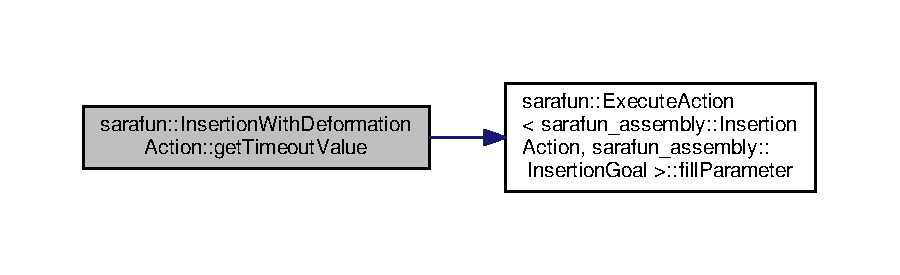
\includegraphics[width=350pt]{d8/db8/classsarafun_1_1InsertionWithDeformationAction_a8d77b104fb2396000b273cb6754ff879_a8d77b104fb2396000b273cb6754ff879_cgraph}
\end{center}
\end{figure}




\subsection{Field Documentation}
\hypertarget{classsarafun_1_1InsertionWithDeformationAction_aa5a6397046e4d8ac145d2961d04fc27c_aa5a6397046e4d8ac145d2961d04fc27c}{\index{sarafun\-::\-Insertion\-With\-Deformation\-Action@{sarafun\-::\-Insertion\-With\-Deformation\-Action}!bt\-\_\-name\-\_\-@{bt\-\_\-name\-\_\-}}
\index{bt\-\_\-name\-\_\-@{bt\-\_\-name\-\_\-}!sarafun::InsertionWithDeformationAction@{sarafun\-::\-Insertion\-With\-Deformation\-Action}}
\subsubsection[{bt\-\_\-name\-\_\-}]{\setlength{\rightskip}{0pt plus 5cm}std\-::string sarafun\-::\-Insertion\-With\-Deformation\-Action\-::bt\-\_\-name\-\_\-\hspace{0.3cm}{\ttfamily [private]}}}\label{classsarafun_1_1InsertionWithDeformationAction_aa5a6397046e4d8ac145d2961d04fc27c_aa5a6397046e4d8ac145d2961d04fc27c}


Definition at line 31 of file Insertion\-With\-Deformation\-Action.\-h.

\hypertarget{classsarafun_1_1InsertionWithDeformationAction_a97fcbe6b19d7f2185e19f5e8397b2307_a97fcbe6b19d7f2185e19f5e8397b2307}{\index{sarafun\-::\-Insertion\-With\-Deformation\-Action@{sarafun\-::\-Insertion\-With\-Deformation\-Action}!node\-\_\-handle\-\_\-@{node\-\_\-handle\-\_\-}}
\index{node\-\_\-handle\-\_\-@{node\-\_\-handle\-\_\-}!sarafun::InsertionWithDeformationAction@{sarafun\-::\-Insertion\-With\-Deformation\-Action}}
\subsubsection[{node\-\_\-handle\-\_\-}]{\setlength{\rightskip}{0pt plus 5cm}ros\-::\-Node\-Handle sarafun\-::\-Insertion\-With\-Deformation\-Action\-::node\-\_\-handle\-\_\-\hspace{0.3cm}{\ttfamily [private]}}}\label{classsarafun_1_1InsertionWithDeformationAction_a97fcbe6b19d7f2185e19f5e8397b2307_a97fcbe6b19d7f2185e19f5e8397b2307}


Definition at line 29 of file Insertion\-With\-Deformation\-Action.\-h.



Referenced by Insertion\-With\-Deformation\-Action().

\hypertarget{classsarafun_1_1InsertionWithDeformationAction_a493a532429347d18fa4d525d982c0204_a493a532429347d18fa4d525d982c0204}{\index{sarafun\-::\-Insertion\-With\-Deformation\-Action@{sarafun\-::\-Insertion\-With\-Deformation\-Action}!node\-\_\-name\-\_\-@{node\-\_\-name\-\_\-}}
\index{node\-\_\-name\-\_\-@{node\-\_\-name\-\_\-}!sarafun::InsertionWithDeformationAction@{sarafun\-::\-Insertion\-With\-Deformation\-Action}}
\subsubsection[{node\-\_\-name\-\_\-}]{\setlength{\rightskip}{0pt plus 5cm}std\-::string sarafun\-::\-Insertion\-With\-Deformation\-Action\-::node\-\_\-name\-\_\-\hspace{0.3cm}{\ttfamily [private]}}}\label{classsarafun_1_1InsertionWithDeformationAction_a493a532429347d18fa4d525d982c0204_a493a532429347d18fa4d525d982c0204}


Definition at line 30 of file Insertion\-With\-Deformation\-Action.\-h.



The documentation for this class was generated from the following files\-:\begin{DoxyCompactItemize}
\item 
Insertion\-With\-Deformation\-Action.\-h\item 
Insertion\-With\-Deformation\-Action.\-cpp\end{DoxyCompactItemize}

\hypertarget{classsarafun_1_1IsSimple}{\section{sarafun\-:\-:Is\-Simple Class Reference}
\label{classsarafun_1_1IsSimple}\index{sarafun\-::\-Is\-Simple@{sarafun\-::\-Is\-Simple}}
}


{\ttfamily \#include $<$Is\-Simple.\-h$>$}



Inherits Condition\-Template.



Collaboration diagram for sarafun\-:\-:Is\-Simple\-:\nopagebreak
\begin{figure}[H]
\begin{center}
\leavevmode
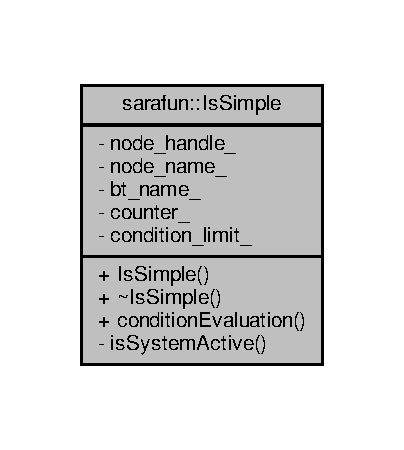
\includegraphics[width=194pt]{de/d41/classsarafun_1_1IsSimple__coll__graph}
\end{center}
\end{figure}
\subsection*{Public Member Functions}
\begin{DoxyCompactItemize}
\item 
\hyperlink{classsarafun_1_1IsSimple_a299c558037426826c95bfc54dbe1a399_a299c558037426826c95bfc54dbe1a399}{Is\-Simple} (std\-::string node\-\_\-name, std\-::string bt\-\_\-name)
\item 
\hyperlink{classsarafun_1_1IsSimple_a90b55180452143b098bfa0f5a184ee58_a90b55180452143b098bfa0f5a184ee58}{$\sim$\-Is\-Simple} ()
\item 
bool \hyperlink{classsarafun_1_1IsSimple_aa57bb3baf9d3ac955e5fdfd5351d45a0_aa57bb3baf9d3ac955e5fdfd5351d45a0}{condition\-Evaluation} ()
\end{DoxyCompactItemize}
\subsection*{Private Member Functions}
\begin{DoxyCompactItemize}
\item 
bool \hyperlink{classsarafun_1_1IsSimple_ac90630b4194e090dfe1e93e7f442576c_ac90630b4194e090dfe1e93e7f442576c}{is\-System\-Active} ()
\end{DoxyCompactItemize}
\subsection*{Private Attributes}
\begin{DoxyCompactItemize}
\item 
ros\-::\-Node\-Handle \hyperlink{classsarafun_1_1IsSimple_a461e5f5f34c94f31f81c11ebd5ccbdc3_a461e5f5f34c94f31f81c11ebd5ccbdc3}{node\-\_\-handle\-\_\-}
\item 
std\-::string \hyperlink{classsarafun_1_1IsSimple_a93a14fccdb5329357b784cb6eb71e2e1_a93a14fccdb5329357b784cb6eb71e2e1}{node\-\_\-name\-\_\-}
\item 
std\-::string \hyperlink{classsarafun_1_1IsSimple_a880440b230fe9b00d396905dbe4dfbc6_a880440b230fe9b00d396905dbe4dfbc6}{bt\-\_\-name\-\_\-}
\item 
int \hyperlink{classsarafun_1_1IsSimple_a57504174276eda97908a4e48b3625a97_a57504174276eda97908a4e48b3625a97}{counter\-\_\-}
\item 
int \hyperlink{classsarafun_1_1IsSimple_aa02f0e66054f68dccf7cc78c763c7141_aa02f0e66054f68dccf7cc78c763c7141}{condition\-\_\-limit\-\_\-}
\end{DoxyCompactItemize}


\subsection{Detailed Description}


Definition at line 8 of file Is\-Simple.\-h.



\subsection{Constructor \& Destructor Documentation}
\hypertarget{classsarafun_1_1IsSimple_a299c558037426826c95bfc54dbe1a399_a299c558037426826c95bfc54dbe1a399}{\index{sarafun\-::\-Is\-Simple@{sarafun\-::\-Is\-Simple}!Is\-Simple@{Is\-Simple}}
\index{Is\-Simple@{Is\-Simple}!sarafun::IsSimple@{sarafun\-::\-Is\-Simple}}
\subsubsection[{Is\-Simple}]{\setlength{\rightskip}{0pt plus 5cm}sarafun\-::\-Is\-Simple\-::\-Is\-Simple (
\begin{DoxyParamCaption}
\item[{std\-::string}]{node\-\_\-name, }
\item[{std\-::string}]{bt\-\_\-name}
\end{DoxyParamCaption}
)\hspace{0.3cm}{\ttfamily [inline]}}}\label{classsarafun_1_1IsSimple_a299c558037426826c95bfc54dbe1a399_a299c558037426826c95bfc54dbe1a399}


Definition at line 10 of file Is\-Simple.\-h.



References bt\-\_\-name\-\_\-, condition\-\_\-limit\-\_\-, counter\-\_\-, and node\-\_\-handle\-\_\-.

\hypertarget{classsarafun_1_1IsSimple_a90b55180452143b098bfa0f5a184ee58_a90b55180452143b098bfa0f5a184ee58}{\index{sarafun\-::\-Is\-Simple@{sarafun\-::\-Is\-Simple}!$\sim$\-Is\-Simple@{$\sim$\-Is\-Simple}}
\index{$\sim$\-Is\-Simple@{$\sim$\-Is\-Simple}!sarafun::IsSimple@{sarafun\-::\-Is\-Simple}}
\subsubsection[{$\sim$\-Is\-Simple}]{\setlength{\rightskip}{0pt plus 5cm}sarafun\-::\-Is\-Simple\-::$\sim$\-Is\-Simple (
\begin{DoxyParamCaption}
{}
\end{DoxyParamCaption}
)\hspace{0.3cm}{\ttfamily [inline]}}}\label{classsarafun_1_1IsSimple_a90b55180452143b098bfa0f5a184ee58_a90b55180452143b098bfa0f5a184ee58}


Definition at line 17 of file Is\-Simple.\-h.



\subsection{Member Function Documentation}
\hypertarget{classsarafun_1_1IsSimple_aa57bb3baf9d3ac955e5fdfd5351d45a0_aa57bb3baf9d3ac955e5fdfd5351d45a0}{\index{sarafun\-::\-Is\-Simple@{sarafun\-::\-Is\-Simple}!condition\-Evaluation@{condition\-Evaluation}}
\index{condition\-Evaluation@{condition\-Evaluation}!sarafun::IsSimple@{sarafun\-::\-Is\-Simple}}
\subsubsection[{condition\-Evaluation}]{\setlength{\rightskip}{0pt plus 5cm}bool sarafun\-::\-Is\-Simple\-::condition\-Evaluation (
\begin{DoxyParamCaption}
{}
\end{DoxyParamCaption}
)}}\label{classsarafun_1_1IsSimple_aa57bb3baf9d3ac955e5fdfd5351d45a0_aa57bb3baf9d3ac955e5fdfd5351d45a0}


Definition at line 20 of file Is\-Simple.\-cpp.



References bt\-\_\-name\-\_\-, condition\-\_\-limit\-\_\-, counter\-\_\-, and is\-System\-Active().



Here is the call graph for this function\-:\nopagebreak
\begin{figure}[H]
\begin{center}
\leavevmode
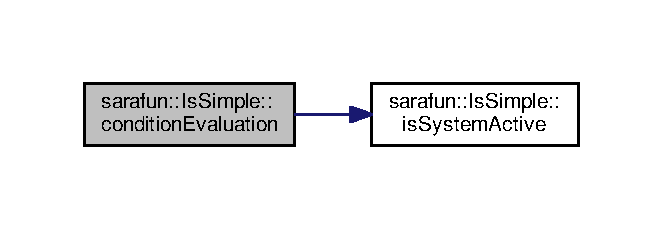
\includegraphics[width=318pt]{dc/d18/classsarafun_1_1IsSimple_aa57bb3baf9d3ac955e5fdfd5351d45a0_aa57bb3baf9d3ac955e5fdfd5351d45a0_cgraph}
\end{center}
\end{figure}


\hypertarget{classsarafun_1_1IsSimple_ac90630b4194e090dfe1e93e7f442576c_ac90630b4194e090dfe1e93e7f442576c}{\index{sarafun\-::\-Is\-Simple@{sarafun\-::\-Is\-Simple}!is\-System\-Active@{is\-System\-Active}}
\index{is\-System\-Active@{is\-System\-Active}!sarafun::IsSimple@{sarafun\-::\-Is\-Simple}}
\subsubsection[{is\-System\-Active}]{\setlength{\rightskip}{0pt plus 5cm}bool sarafun\-::\-Is\-Simple\-::is\-System\-Active (
\begin{DoxyParamCaption}
{}
\end{DoxyParamCaption}
)\hspace{0.3cm}{\ttfamily [private]}}}\label{classsarafun_1_1IsSimple_ac90630b4194e090dfe1e93e7f442576c_ac90630b4194e090dfe1e93e7f442576c}


Definition at line 5 of file Is\-Simple.\-cpp.



Referenced by condition\-Evaluation().



\subsection{Field Documentation}
\hypertarget{classsarafun_1_1IsSimple_a880440b230fe9b00d396905dbe4dfbc6_a880440b230fe9b00d396905dbe4dfbc6}{\index{sarafun\-::\-Is\-Simple@{sarafun\-::\-Is\-Simple}!bt\-\_\-name\-\_\-@{bt\-\_\-name\-\_\-}}
\index{bt\-\_\-name\-\_\-@{bt\-\_\-name\-\_\-}!sarafun::IsSimple@{sarafun\-::\-Is\-Simple}}
\subsubsection[{bt\-\_\-name\-\_\-}]{\setlength{\rightskip}{0pt plus 5cm}std\-::string sarafun\-::\-Is\-Simple\-::bt\-\_\-name\-\_\-\hspace{0.3cm}{\ttfamily [private]}}}\label{classsarafun_1_1IsSimple_a880440b230fe9b00d396905dbe4dfbc6_a880440b230fe9b00d396905dbe4dfbc6}


Definition at line 24 of file Is\-Simple.\-h.



Referenced by condition\-Evaluation(), and Is\-Simple().

\hypertarget{classsarafun_1_1IsSimple_aa02f0e66054f68dccf7cc78c763c7141_aa02f0e66054f68dccf7cc78c763c7141}{\index{sarafun\-::\-Is\-Simple@{sarafun\-::\-Is\-Simple}!condition\-\_\-limit\-\_\-@{condition\-\_\-limit\-\_\-}}
\index{condition\-\_\-limit\-\_\-@{condition\-\_\-limit\-\_\-}!sarafun::IsSimple@{sarafun\-::\-Is\-Simple}}
\subsubsection[{condition\-\_\-limit\-\_\-}]{\setlength{\rightskip}{0pt plus 5cm}int sarafun\-::\-Is\-Simple\-::condition\-\_\-limit\-\_\-\hspace{0.3cm}{\ttfamily [private]}}}\label{classsarafun_1_1IsSimple_aa02f0e66054f68dccf7cc78c763c7141_aa02f0e66054f68dccf7cc78c763c7141}


Definition at line 26 of file Is\-Simple.\-h.



Referenced by condition\-Evaluation(), and Is\-Simple().

\hypertarget{classsarafun_1_1IsSimple_a57504174276eda97908a4e48b3625a97_a57504174276eda97908a4e48b3625a97}{\index{sarafun\-::\-Is\-Simple@{sarafun\-::\-Is\-Simple}!counter\-\_\-@{counter\-\_\-}}
\index{counter\-\_\-@{counter\-\_\-}!sarafun::IsSimple@{sarafun\-::\-Is\-Simple}}
\subsubsection[{counter\-\_\-}]{\setlength{\rightskip}{0pt plus 5cm}int sarafun\-::\-Is\-Simple\-::counter\-\_\-\hspace{0.3cm}{\ttfamily [private]}}}\label{classsarafun_1_1IsSimple_a57504174276eda97908a4e48b3625a97_a57504174276eda97908a4e48b3625a97}


Definition at line 26 of file Is\-Simple.\-h.



Referenced by condition\-Evaluation(), and Is\-Simple().

\hypertarget{classsarafun_1_1IsSimple_a461e5f5f34c94f31f81c11ebd5ccbdc3_a461e5f5f34c94f31f81c11ebd5ccbdc3}{\index{sarafun\-::\-Is\-Simple@{sarafun\-::\-Is\-Simple}!node\-\_\-handle\-\_\-@{node\-\_\-handle\-\_\-}}
\index{node\-\_\-handle\-\_\-@{node\-\_\-handle\-\_\-}!sarafun::IsSimple@{sarafun\-::\-Is\-Simple}}
\subsubsection[{node\-\_\-handle\-\_\-}]{\setlength{\rightskip}{0pt plus 5cm}ros\-::\-Node\-Handle sarafun\-::\-Is\-Simple\-::node\-\_\-handle\-\_\-\hspace{0.3cm}{\ttfamily [private]}}}\label{classsarafun_1_1IsSimple_a461e5f5f34c94f31f81c11ebd5ccbdc3_a461e5f5f34c94f31f81c11ebd5ccbdc3}


Definition at line 22 of file Is\-Simple.\-h.



Referenced by Is\-Simple().

\hypertarget{classsarafun_1_1IsSimple_a93a14fccdb5329357b784cb6eb71e2e1_a93a14fccdb5329357b784cb6eb71e2e1}{\index{sarafun\-::\-Is\-Simple@{sarafun\-::\-Is\-Simple}!node\-\_\-name\-\_\-@{node\-\_\-name\-\_\-}}
\index{node\-\_\-name\-\_\-@{node\-\_\-name\-\_\-}!sarafun::IsSimple@{sarafun\-::\-Is\-Simple}}
\subsubsection[{node\-\_\-name\-\_\-}]{\setlength{\rightskip}{0pt plus 5cm}std\-::string sarafun\-::\-Is\-Simple\-::node\-\_\-name\-\_\-\hspace{0.3cm}{\ttfamily [private]}}}\label{classsarafun_1_1IsSimple_a93a14fccdb5329357b784cb6eb71e2e1_a93a14fccdb5329357b784cb6eb71e2e1}


Definition at line 23 of file Is\-Simple.\-h.



The documentation for this class was generated from the following files\-:\begin{DoxyCompactItemize}
\item 
Is\-Simple.\-h\item 
Is\-Simple.\-cpp\end{DoxyCompactItemize}

\hypertarget{classsarafun_1_1MoveAction}{\section{sarafun\-:\-:Move\-Action Class Reference}
\label{classsarafun_1_1MoveAction}\index{sarafun\-::\-Move\-Action@{sarafun\-::\-Move\-Action}}
}


{\ttfamily \#include $<$Move\-Action.\-h$>$}

Inheritance diagram for sarafun\-:\-:Move\-Action\-:\begin{figure}[H]
\begin{center}
\leavevmode
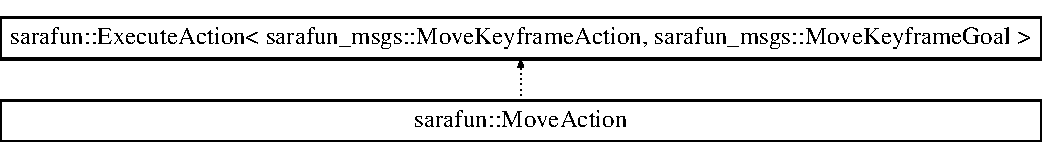
\includegraphics[height=1.914530cm]{classsarafun_1_1MoveAction}
\end{center}
\end{figure}
\subsection*{Public Member Functions}
\begin{DoxyCompactItemize}
\item 
\hyperlink{classsarafun_1_1MoveAction_a423d16aa9d5a47e9f558eae9e013c5e7}{Move\-Action} (std\-::string node\-\_\-name, std\-::string action\-\_\-name, std\-::string bt\-\_\-name)
\item 
\hyperlink{classsarafun_1_1MoveAction_ab9b7f0e483bd9a0b53f9651d661c93b7}{$\sim$\-Move\-Action} ()
\item 
bool \hyperlink{classsarafun_1_1MoveAction_ad5259389b6a5718389c24fab920c9296}{fill\-Goal} (sarafun\-\_\-msgs\-::\-Move\-Keyframe\-Goal \&goal)
\item 
double \hyperlink{classsarafun_1_1MoveAction_a3a0d4d2919b30b878c603a884db6a470}{get\-Timeout\-Value} ()
\end{DoxyCompactItemize}


\subsection{Constructor \& Destructor Documentation}
\hypertarget{classsarafun_1_1MoveAction_a423d16aa9d5a47e9f558eae9e013c5e7}{\index{sarafun\-::\-Move\-Action@{sarafun\-::\-Move\-Action}!Move\-Action@{Move\-Action}}
\index{Move\-Action@{Move\-Action}!sarafun::MoveAction@{sarafun\-::\-Move\-Action}}
\subsubsection[{Move\-Action}]{\setlength{\rightskip}{0pt plus 5cm}sarafun\-::\-Move\-Action\-::\-Move\-Action (
\begin{DoxyParamCaption}
\item[{std\-::string}]{node\-\_\-name, }
\item[{std\-::string}]{action\-\_\-name, }
\item[{std\-::string}]{bt\-\_\-name}
\end{DoxyParamCaption}
)\hspace{0.3cm}{\ttfamily [inline]}}}\label{classsarafun_1_1MoveAction_a423d16aa9d5a47e9f558eae9e013c5e7}
\hypertarget{classsarafun_1_1MoveAction_ab9b7f0e483bd9a0b53f9651d661c93b7}{\index{sarafun\-::\-Move\-Action@{sarafun\-::\-Move\-Action}!$\sim$\-Move\-Action@{$\sim$\-Move\-Action}}
\index{$\sim$\-Move\-Action@{$\sim$\-Move\-Action}!sarafun::MoveAction@{sarafun\-::\-Move\-Action}}
\subsubsection[{$\sim$\-Move\-Action}]{\setlength{\rightskip}{0pt plus 5cm}sarafun\-::\-Move\-Action\-::$\sim$\-Move\-Action (
\begin{DoxyParamCaption}
{}
\end{DoxyParamCaption}
)\hspace{0.3cm}{\ttfamily [inline]}}}\label{classsarafun_1_1MoveAction_ab9b7f0e483bd9a0b53f9651d661c93b7}


\subsection{Member Function Documentation}
\hypertarget{classsarafun_1_1MoveAction_ad5259389b6a5718389c24fab920c9296}{\index{sarafun\-::\-Move\-Action@{sarafun\-::\-Move\-Action}!fill\-Goal@{fill\-Goal}}
\index{fill\-Goal@{fill\-Goal}!sarafun::MoveAction@{sarafun\-::\-Move\-Action}}
\subsubsection[{fill\-Goal}]{\setlength{\rightskip}{0pt plus 5cm}bool sarafun\-::\-Move\-Action\-::fill\-Goal (
\begin{DoxyParamCaption}
\item[{sarafun\-\_\-msgs\-::\-Move\-Keyframe\-Goal \&}]{goal}
\end{DoxyParamCaption}
)\hspace{0.3cm}{\ttfamily [virtual]}}}\label{classsarafun_1_1MoveAction_ad5259389b6a5718389c24fab920c9296}
Fills in the goal for a particular action.


\begin{DoxyParams}{Parameters}
{\em goal} & The actionlib goal message of the externally implemented action. \\
\hline
\end{DoxyParams}
\begin{DoxyReturn}{Returns}
False in case of error, true otherwise. 
\end{DoxyReturn}


Implements \hyperlink{classsarafun_1_1ExecuteAction_a6dd9c0f013d15a17d7e7ce8dbe40a436}{sarafun\-::\-Execute\-Action$<$ sarafun\-\_\-msgs\-::\-Move\-Keyframe\-Action, sarafun\-\_\-msgs\-::\-Move\-Keyframe\-Goal $>$}.

\hypertarget{classsarafun_1_1MoveAction_a3a0d4d2919b30b878c603a884db6a470}{\index{sarafun\-::\-Move\-Action@{sarafun\-::\-Move\-Action}!get\-Timeout\-Value@{get\-Timeout\-Value}}
\index{get\-Timeout\-Value@{get\-Timeout\-Value}!sarafun::MoveAction@{sarafun\-::\-Move\-Action}}
\subsubsection[{get\-Timeout\-Value}]{\setlength{\rightskip}{0pt plus 5cm}double sarafun\-::\-Move\-Action\-::get\-Timeout\-Value (
\begin{DoxyParamCaption}
{}
\end{DoxyParamCaption}
)\hspace{0.3cm}{\ttfamily [virtual]}}}\label{classsarafun_1_1MoveAction_a3a0d4d2919b30b878c603a884db6a470}
Provides the client with a timeout value for actionlib connections.

\begin{DoxyReturn}{Returns}
The timeout value (in seconds). 
\end{DoxyReturn}


Implements \hyperlink{classsarafun_1_1ExecuteAction_aba6cfa8a8ce19e735eb6394424df6d17}{sarafun\-::\-Execute\-Action$<$ sarafun\-\_\-msgs\-::\-Move\-Keyframe\-Action, sarafun\-\_\-msgs\-::\-Move\-Keyframe\-Goal $>$}.



The documentation for this class was generated from the following files\-:\begin{DoxyCompactItemize}
\item 
sarafun\-\_\-tree/include/sarafun\-\_\-tree/sarafun\-\_\-action\-\_\-nodes/\hyperlink{MoveAction_8h}{Move\-Action.\-h}\item 
sarafun\-\_\-tree/src/sarafun\-\_\-action\-\_\-nodes/\hyperlink{MoveAction_8cpp}{Move\-Action.\-cpp}\end{DoxyCompactItemize}

\hypertarget{classsarafun_1_1OnlineMotionAction}{\section{sarafun\-:\-:Online\-Motion\-Action Class Reference}
\label{classsarafun_1_1OnlineMotionAction}\index{sarafun\-::\-Online\-Motion\-Action@{sarafun\-::\-Online\-Motion\-Action}}
}


{\ttfamily \#include $<$Online\-Motion\-Action.\-h$>$}

Inheritance diagram for sarafun\-:\-:Online\-Motion\-Action\-:\begin{figure}[H]
\begin{center}
\leavevmode
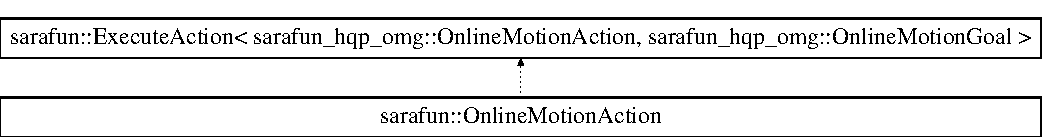
\includegraphics[height=1.845140cm]{classsarafun_1_1OnlineMotionAction}
\end{center}
\end{figure}
\subsection*{Public Member Functions}
\begin{DoxyCompactItemize}
\item 
\hyperlink{classsarafun_1_1OnlineMotionAction_ab66225e6e9383411dc925e88fb1cf4f9}{Online\-Motion\-Action} (std\-::string node\-\_\-name, std\-::string action\-\_\-name, std\-::string bt\-\_\-name)
\item 
\hyperlink{classsarafun_1_1OnlineMotionAction_a63134a65e9ead7a8250abe2afee5b388}{$\sim$\-Online\-Motion\-Action} ()
\item 
bool \hyperlink{classsarafun_1_1OnlineMotionAction_aacaa264dad7ba07b5c9a985d66ea48f7}{fill\-Goal} (sarafun\-\_\-hqp\-\_\-omg\-::\-Online\-Motion\-Goal \&goal)
\item 
double \hyperlink{classsarafun_1_1OnlineMotionAction_a453e7dca41a0d73b5297ce191e760b31}{get\-Timeout\-Value} ()
\end{DoxyCompactItemize}


\subsection{Constructor \& Destructor Documentation}
\hypertarget{classsarafun_1_1OnlineMotionAction_ab66225e6e9383411dc925e88fb1cf4f9}{\index{sarafun\-::\-Online\-Motion\-Action@{sarafun\-::\-Online\-Motion\-Action}!Online\-Motion\-Action@{Online\-Motion\-Action}}
\index{Online\-Motion\-Action@{Online\-Motion\-Action}!sarafun::OnlineMotionAction@{sarafun\-::\-Online\-Motion\-Action}}
\subsubsection[{Online\-Motion\-Action}]{\setlength{\rightskip}{0pt plus 5cm}sarafun\-::\-Online\-Motion\-Action\-::\-Online\-Motion\-Action (
\begin{DoxyParamCaption}
\item[{std\-::string}]{node\-\_\-name, }
\item[{std\-::string}]{action\-\_\-name, }
\item[{std\-::string}]{bt\-\_\-name}
\end{DoxyParamCaption}
)\hspace{0.3cm}{\ttfamily [inline]}}}\label{classsarafun_1_1OnlineMotionAction_ab66225e6e9383411dc925e88fb1cf4f9}
\hypertarget{classsarafun_1_1OnlineMotionAction_a63134a65e9ead7a8250abe2afee5b388}{\index{sarafun\-::\-Online\-Motion\-Action@{sarafun\-::\-Online\-Motion\-Action}!$\sim$\-Online\-Motion\-Action@{$\sim$\-Online\-Motion\-Action}}
\index{$\sim$\-Online\-Motion\-Action@{$\sim$\-Online\-Motion\-Action}!sarafun::OnlineMotionAction@{sarafun\-::\-Online\-Motion\-Action}}
\subsubsection[{$\sim$\-Online\-Motion\-Action}]{\setlength{\rightskip}{0pt plus 5cm}sarafun\-::\-Online\-Motion\-Action\-::$\sim$\-Online\-Motion\-Action (
\begin{DoxyParamCaption}
{}
\end{DoxyParamCaption}
)\hspace{0.3cm}{\ttfamily [inline]}}}\label{classsarafun_1_1OnlineMotionAction_a63134a65e9ead7a8250abe2afee5b388}


\subsection{Member Function Documentation}
\hypertarget{classsarafun_1_1OnlineMotionAction_aacaa264dad7ba07b5c9a985d66ea48f7}{\index{sarafun\-::\-Online\-Motion\-Action@{sarafun\-::\-Online\-Motion\-Action}!fill\-Goal@{fill\-Goal}}
\index{fill\-Goal@{fill\-Goal}!sarafun::OnlineMotionAction@{sarafun\-::\-Online\-Motion\-Action}}
\subsubsection[{fill\-Goal}]{\setlength{\rightskip}{0pt plus 5cm}bool sarafun\-::\-Online\-Motion\-Action\-::fill\-Goal (
\begin{DoxyParamCaption}
\item[{sarafun\-\_\-hqp\-\_\-omg\-::\-Online\-Motion\-Goal \&}]{goal}
\end{DoxyParamCaption}
)\hspace{0.3cm}{\ttfamily [virtual]}}}\label{classsarafun_1_1OnlineMotionAction_aacaa264dad7ba07b5c9a985d66ea48f7}
Fills in the goal for a particular action.


\begin{DoxyParams}{Parameters}
{\em goal} & The actionlib goal message of the externally implemented action. \\
\hline
\end{DoxyParams}
\begin{DoxyReturn}{Returns}
False in case of error, true otherwise. 
\end{DoxyReturn}


Implements \hyperlink{classsarafun_1_1ExecuteAction_a6dd9c0f013d15a17d7e7ce8dbe40a436}{sarafun\-::\-Execute\-Action$<$ sarafun\-\_\-hqp\-\_\-omg\-::\-Online\-Motion\-Action, sarafun\-\_\-hqp\-\_\-omg\-::\-Online\-Motion\-Goal $>$}.

\hypertarget{classsarafun_1_1OnlineMotionAction_a453e7dca41a0d73b5297ce191e760b31}{\index{sarafun\-::\-Online\-Motion\-Action@{sarafun\-::\-Online\-Motion\-Action}!get\-Timeout\-Value@{get\-Timeout\-Value}}
\index{get\-Timeout\-Value@{get\-Timeout\-Value}!sarafun::OnlineMotionAction@{sarafun\-::\-Online\-Motion\-Action}}
\subsubsection[{get\-Timeout\-Value}]{\setlength{\rightskip}{0pt plus 5cm}double sarafun\-::\-Online\-Motion\-Action\-::get\-Timeout\-Value (
\begin{DoxyParamCaption}
{}
\end{DoxyParamCaption}
)\hspace{0.3cm}{\ttfamily [virtual]}}}\label{classsarafun_1_1OnlineMotionAction_a453e7dca41a0d73b5297ce191e760b31}
Provides the client with a timeout value for actionlib connections.

\begin{DoxyReturn}{Returns}
The timeout value (in seconds). 
\end{DoxyReturn}


Implements \hyperlink{classsarafun_1_1ExecuteAction_aba6cfa8a8ce19e735eb6394424df6d17}{sarafun\-::\-Execute\-Action$<$ sarafun\-\_\-hqp\-\_\-omg\-::\-Online\-Motion\-Action, sarafun\-\_\-hqp\-\_\-omg\-::\-Online\-Motion\-Goal $>$}.



The documentation for this class was generated from the following files\-:\begin{DoxyCompactItemize}
\item 
sarafun\-\_\-tree/include/sarafun\-\_\-tree/demo\-\_\-bt\-\_\-nodes/\hyperlink{OnlineMotionAction_8h}{Online\-Motion\-Action.\-h}\item 
sarafun\-\_\-tree/src/demo\-\_\-bt\-\_\-nodes/\hyperlink{OnlineMotionAction_8cpp}{Online\-Motion\-Action.\-cpp}\end{DoxyCompactItemize}

\hypertarget{classbt__parser_1_1Parser}{\section{bt\-\_\-parser\-:\-:Parser Class Reference}
\label{classbt__parser_1_1Parser}\index{bt\-\_\-parser\-::\-Parser@{bt\-\_\-parser\-::\-Parser}}
}


{\ttfamily \#include $<$parse\-\_\-tree.\-h$>$}



Collaboration diagram for bt\-\_\-parser\-:\-:Parser\-:\nopagebreak
\begin{figure}[H]
\begin{center}
\leavevmode
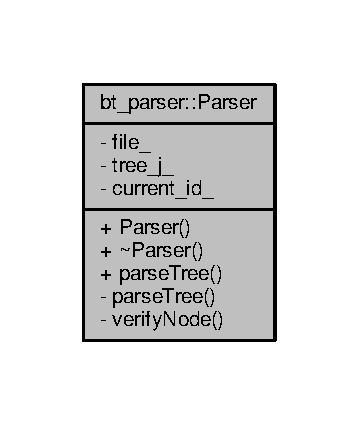
\includegraphics[width=172pt]{d2/d92/classbt__parser_1_1Parser__coll__graph}
\end{center}
\end{figure}
\subsection*{Public Member Functions}
\begin{DoxyCompactItemize}
\item 
\hyperlink{classbt__parser_1_1Parser_abcd6235386f006f36b56ceb08c898deb_abcd6235386f006f36b56ceb08c898deb}{Parser} (std\-::string filepath)
\item 
\hyperlink{classbt__parser_1_1Parser_a5a8992b935e01bac1fa36da4d20eb718_a5a8992b935e01bac1fa36da4d20eb718}{$\sim$\-Parser} ()
\item 
B\-T\-::\-Tree\-Node $\ast$ \hyperlink{classbt__parser_1_1Parser_a7c744cc625df4ce26fbaa3deba496737_a7c744cc625df4ce26fbaa3deba496737}{parse\-Tree} ()
\end{DoxyCompactItemize}
\subsection*{Private Member Functions}
\begin{DoxyCompactItemize}
\item 
B\-T\-::\-Tree\-Node $\ast$ \hyperlink{classbt__parser_1_1Parser_a30c924ebeff1273b8612c41bd5e7ffe2_a30c924ebeff1273b8612c41bd5e7ffe2}{parse\-Tree} (json node)
\item 
void \hyperlink{classbt__parser_1_1Parser_a67d8ea4c25f3088b8e5b18cc01837d1a_a67d8ea4c25f3088b8e5b18cc01837d1a}{verify\-Node} (json node)
\end{DoxyCompactItemize}
\subsection*{Private Attributes}
\begin{DoxyCompactItemize}
\item 
std\-::ifstream \hyperlink{classbt__parser_1_1Parser_a2f2c7b9fcfd823c22b8e4385e8e2ce63_a2f2c7b9fcfd823c22b8e4385e8e2ce63}{file\-\_\-}
\item 
json \hyperlink{classbt__parser_1_1Parser_abd894df8a1d8c0aaf660fc02ca1f3882_abd894df8a1d8c0aaf660fc02ca1f3882}{tree\-\_\-j\-\_\-}
\item 
std\-::string \hyperlink{classbt__parser_1_1Parser_a8a2cd4996ff4cc8a6de26caa52756620_a8a2cd4996ff4cc8a6de26caa52756620}{current\-\_\-id\-\_\-}
\end{DoxyCompactItemize}


\subsection{Detailed Description}
Implements a behavior tree parser, that reads a J\-S\-O\-N file describing the tree and generates the executable tree structure. 

Definition at line 17 of file parse\-\_\-tree.\-h.



\subsection{Constructor \& Destructor Documentation}
\hypertarget{classbt__parser_1_1Parser_abcd6235386f006f36b56ceb08c898deb_abcd6235386f006f36b56ceb08c898deb}{\index{bt\-\_\-parser\-::\-Parser@{bt\-\_\-parser\-::\-Parser}!Parser@{Parser}}
\index{Parser@{Parser}!bt_parser::Parser@{bt\-\_\-parser\-::\-Parser}}
\subsubsection[{Parser}]{\setlength{\rightskip}{0pt plus 5cm}bt\-\_\-parser\-::\-Parser\-::\-Parser (
\begin{DoxyParamCaption}
\item[{std\-::string}]{filepath}
\end{DoxyParamCaption}
)}}\label{classbt__parser_1_1Parser_abcd6235386f006f36b56ceb08c898deb_abcd6235386f006f36b56ceb08c898deb}

\begin{DoxyParams}{Parameters}
{\em filepath} & The directory of the J\-S\-O\-N tree description. \\
\hline
\end{DoxyParams}


Definition at line 5 of file parse\-\_\-tree.\-cpp.



References file\-\_\-.

\hypertarget{classbt__parser_1_1Parser_a5a8992b935e01bac1fa36da4d20eb718_a5a8992b935e01bac1fa36da4d20eb718}{\index{bt\-\_\-parser\-::\-Parser@{bt\-\_\-parser\-::\-Parser}!$\sim$\-Parser@{$\sim$\-Parser}}
\index{$\sim$\-Parser@{$\sim$\-Parser}!bt_parser::Parser@{bt\-\_\-parser\-::\-Parser}}
\subsubsection[{$\sim$\-Parser}]{\setlength{\rightskip}{0pt plus 5cm}bt\-\_\-parser\-::\-Parser\-::$\sim$\-Parser (
\begin{DoxyParamCaption}
{}
\end{DoxyParamCaption}
)}}\label{classbt__parser_1_1Parser_a5a8992b935e01bac1fa36da4d20eb718_a5a8992b935e01bac1fa36da4d20eb718}


Definition at line 6 of file parse\-\_\-tree.\-cpp.



References file\-\_\-.



\subsection{Member Function Documentation}
\hypertarget{classbt__parser_1_1Parser_a7c744cc625df4ce26fbaa3deba496737_a7c744cc625df4ce26fbaa3deba496737}{\index{bt\-\_\-parser\-::\-Parser@{bt\-\_\-parser\-::\-Parser}!parse\-Tree@{parse\-Tree}}
\index{parse\-Tree@{parse\-Tree}!bt_parser::Parser@{bt\-\_\-parser\-::\-Parser}}
\subsubsection[{parse\-Tree}]{\setlength{\rightskip}{0pt plus 5cm}B\-T\-::\-Tree\-Node $\ast$ bt\-\_\-parser\-::\-Parser\-::parse\-Tree (
\begin{DoxyParamCaption}
{}
\end{DoxyParamCaption}
)}}\label{classbt__parser_1_1Parser_a7c744cc625df4ce26fbaa3deba496737_a7c744cc625df4ce26fbaa3deba496737}


Definition at line 29 of file parse\-\_\-tree.\-cpp.



References current\-\_\-id\-\_\-, file\-\_\-, and tree\-\_\-j\-\_\-.



Referenced by parse\-Tree().

\hypertarget{classbt__parser_1_1Parser_a30c924ebeff1273b8612c41bd5e7ffe2_a30c924ebeff1273b8612c41bd5e7ffe2}{\index{bt\-\_\-parser\-::\-Parser@{bt\-\_\-parser\-::\-Parser}!parse\-Tree@{parse\-Tree}}
\index{parse\-Tree@{parse\-Tree}!bt_parser::Parser@{bt\-\_\-parser\-::\-Parser}}
\subsubsection[{parse\-Tree}]{\setlength{\rightskip}{0pt plus 5cm}B\-T\-::\-Tree\-Node $\ast$ bt\-\_\-parser\-::\-Parser\-::parse\-Tree (
\begin{DoxyParamCaption}
\item[{json}]{node}
\end{DoxyParamCaption}
)\hspace{0.3cm}{\ttfamily [private]}}}\label{classbt__parser_1_1Parser_a30c924ebeff1273b8612c41bd5e7ffe2_a30c924ebeff1273b8612c41bd5e7ffe2}


Definition at line 56 of file parse\-\_\-tree.\-cpp.



References current\-\_\-id\-\_\-, parse\-Tree(), tree\-\_\-j\-\_\-, and verify\-Node().



Here is the call graph for this function\-:\nopagebreak
\begin{figure}[H]
\begin{center}
\leavevmode
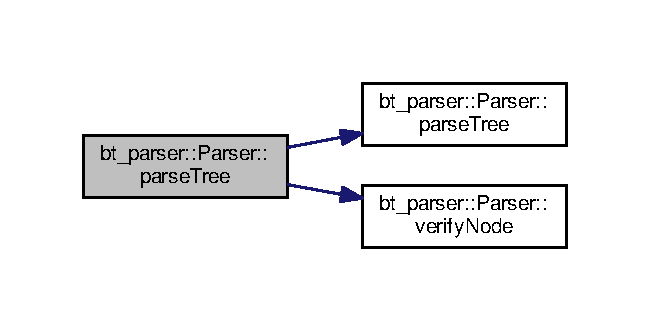
\includegraphics[width=312pt]{dd/d2f/classbt__parser_1_1Parser_a30c924ebeff1273b8612c41bd5e7ffe2_a30c924ebeff1273b8612c41bd5e7ffe2_cgraph}
\end{center}
\end{figure}


\hypertarget{classbt__parser_1_1Parser_a67d8ea4c25f3088b8e5b18cc01837d1a_a67d8ea4c25f3088b8e5b18cc01837d1a}{\index{bt\-\_\-parser\-::\-Parser@{bt\-\_\-parser\-::\-Parser}!verify\-Node@{verify\-Node}}
\index{verify\-Node@{verify\-Node}!bt_parser::Parser@{bt\-\_\-parser\-::\-Parser}}
\subsubsection[{verify\-Node}]{\setlength{\rightskip}{0pt plus 5cm}void bt\-\_\-parser\-::\-Parser\-::verify\-Node (
\begin{DoxyParamCaption}
\item[{json}]{node}
\end{DoxyParamCaption}
)\hspace{0.3cm}{\ttfamily [private]}}}\label{classbt__parser_1_1Parser_a67d8ea4c25f3088b8e5b18cc01837d1a_a67d8ea4c25f3088b8e5b18cc01837d1a}
Verifies the sanity of the given J\-S\-O\-N node describing a B\-T subtree.


\begin{DoxyParams}{Parameters}
{\em node} & A json node object with a B\-T subtree. \\
\hline
\end{DoxyParams}

\begin{DoxyExceptions}{Exceptions}
{\em logic\-\_\-error} & \\
\hline
\end{DoxyExceptions}


Definition at line 8 of file parse\-\_\-tree.\-cpp.



Referenced by parse\-Tree().



\subsection{Field Documentation}
\hypertarget{classbt__parser_1_1Parser_a8a2cd4996ff4cc8a6de26caa52756620_a8a2cd4996ff4cc8a6de26caa52756620}{\index{bt\-\_\-parser\-::\-Parser@{bt\-\_\-parser\-::\-Parser}!current\-\_\-id\-\_\-@{current\-\_\-id\-\_\-}}
\index{current\-\_\-id\-\_\-@{current\-\_\-id\-\_\-}!bt_parser::Parser@{bt\-\_\-parser\-::\-Parser}}
\subsubsection[{current\-\_\-id\-\_\-}]{\setlength{\rightskip}{0pt plus 5cm}std\-::string bt\-\_\-parser\-::\-Parser\-::current\-\_\-id\-\_\-\hspace{0.3cm}{\ttfamily [private]}}}\label{classbt__parser_1_1Parser_a8a2cd4996ff4cc8a6de26caa52756620_a8a2cd4996ff4cc8a6de26caa52756620}


Definition at line 36 of file parse\-\_\-tree.\-h.



Referenced by parse\-Tree().

\hypertarget{classbt__parser_1_1Parser_a2f2c7b9fcfd823c22b8e4385e8e2ce63_a2f2c7b9fcfd823c22b8e4385e8e2ce63}{\index{bt\-\_\-parser\-::\-Parser@{bt\-\_\-parser\-::\-Parser}!file\-\_\-@{file\-\_\-}}
\index{file\-\_\-@{file\-\_\-}!bt_parser::Parser@{bt\-\_\-parser\-::\-Parser}}
\subsubsection[{file\-\_\-}]{\setlength{\rightskip}{0pt plus 5cm}std\-::ifstream bt\-\_\-parser\-::\-Parser\-::file\-\_\-\hspace{0.3cm}{\ttfamily [private]}}}\label{classbt__parser_1_1Parser_a2f2c7b9fcfd823c22b8e4385e8e2ce63_a2f2c7b9fcfd823c22b8e4385e8e2ce63}


Definition at line 34 of file parse\-\_\-tree.\-h.



Referenced by Parser(), parse\-Tree(), and $\sim$\-Parser().

\hypertarget{classbt__parser_1_1Parser_abd894df8a1d8c0aaf660fc02ca1f3882_abd894df8a1d8c0aaf660fc02ca1f3882}{\index{bt\-\_\-parser\-::\-Parser@{bt\-\_\-parser\-::\-Parser}!tree\-\_\-j\-\_\-@{tree\-\_\-j\-\_\-}}
\index{tree\-\_\-j\-\_\-@{tree\-\_\-j\-\_\-}!bt_parser::Parser@{bt\-\_\-parser\-::\-Parser}}
\subsubsection[{tree\-\_\-j\-\_\-}]{\setlength{\rightskip}{0pt plus 5cm}json bt\-\_\-parser\-::\-Parser\-::tree\-\_\-j\-\_\-\hspace{0.3cm}{\ttfamily [private]}}}\label{classbt__parser_1_1Parser_abd894df8a1d8c0aaf660fc02ca1f3882_abd894df8a1d8c0aaf660fc02ca1f3882}


Definition at line 35 of file parse\-\_\-tree.\-h.



Referenced by parse\-Tree().



The documentation for this class was generated from the following files\-:\begin{DoxyCompactItemize}
\item 
parse\-\_\-tree.\-h\item 
parse\-\_\-tree.\-cpp\end{DoxyCompactItemize}

\hypertarget{classsarafun_1_1PickupAction}{\section{sarafun\-:\-:Pickup\-Action Class Reference}
\label{classsarafun_1_1PickupAction}\index{sarafun\-::\-Pickup\-Action@{sarafun\-::\-Pickup\-Action}}
}


{\ttfamily \#include $<$Pickup\-Action.\-h$>$}



Inheritance diagram for sarafun\-:\-:Pickup\-Action\-:
\nopagebreak
\begin{figure}[H]
\begin{center}
\leavevmode
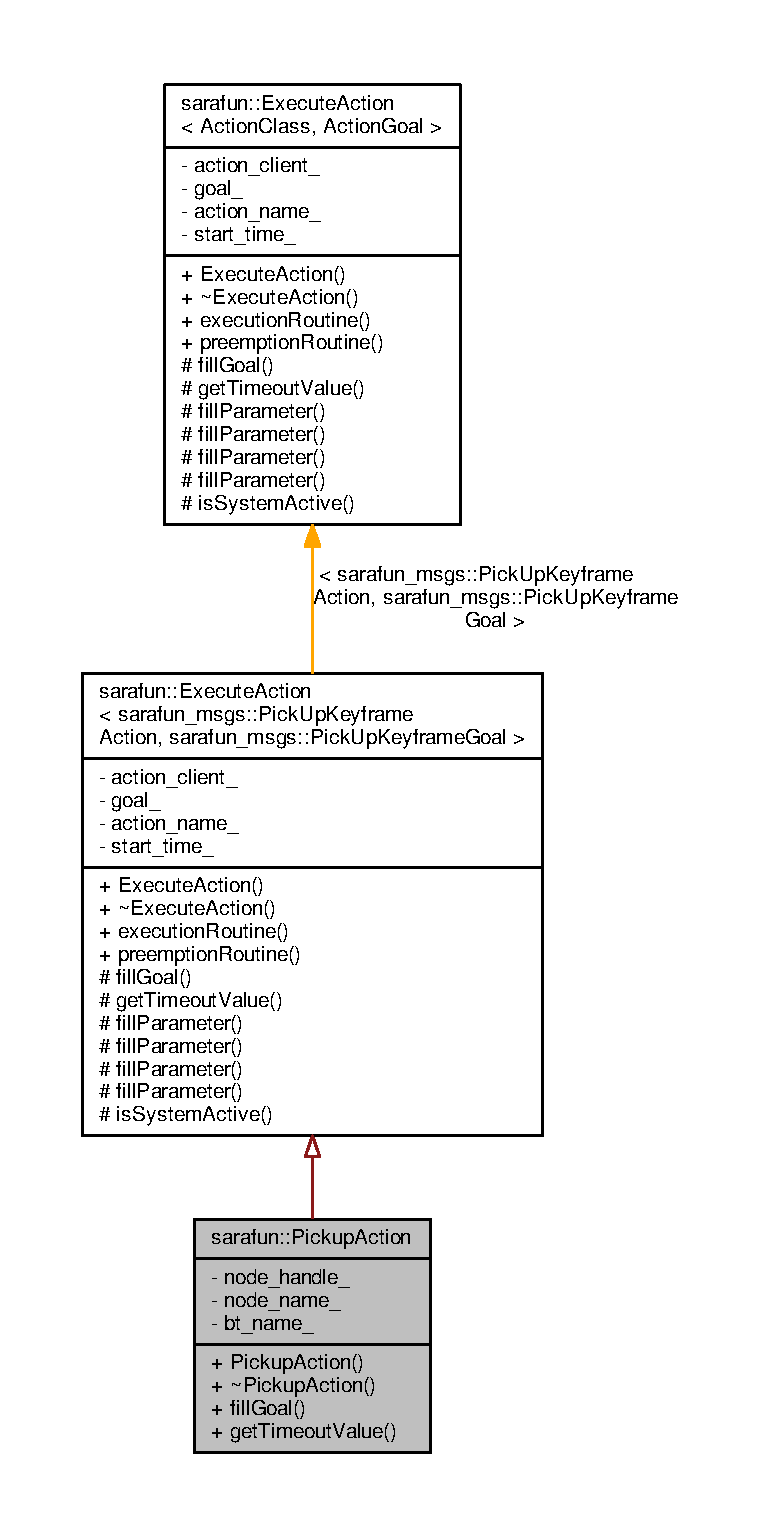
\includegraphics[height=550pt]{db/de1/classsarafun_1_1PickupAction__inherit__graph}
\end{center}
\end{figure}


Collaboration diagram for sarafun\-:\-:Pickup\-Action\-:
\nopagebreak
\begin{figure}[H]
\begin{center}
\leavevmode
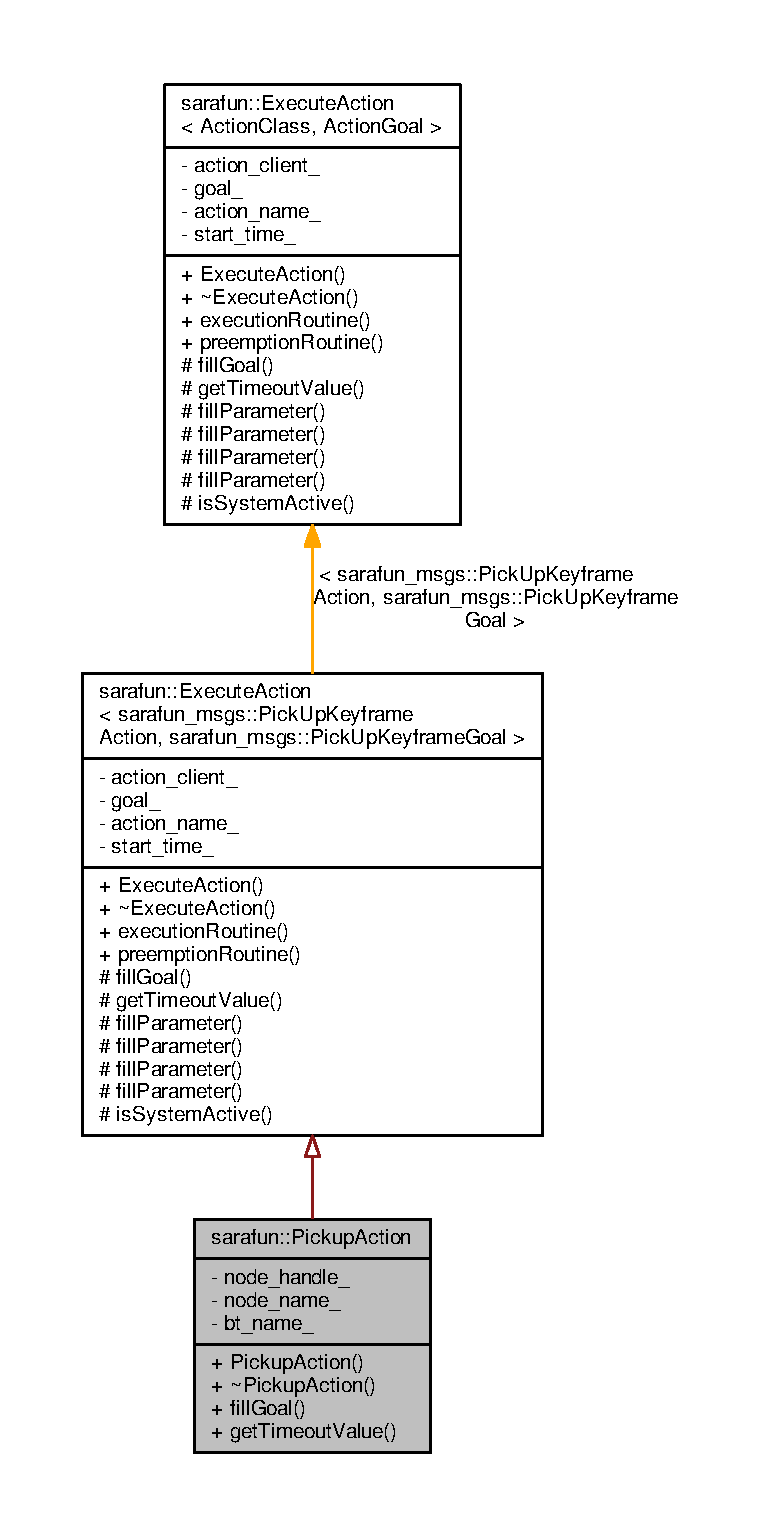
\includegraphics[height=550pt]{d5/da2/classsarafun_1_1PickupAction__coll__graph}
\end{center}
\end{figure}
\subsection*{Public Member Functions}
\begin{DoxyCompactItemize}
\item 
\hyperlink{classsarafun_1_1PickupAction_a1663ebd551413acbc5f21e86a0e3b8cc_a1663ebd551413acbc5f21e86a0e3b8cc}{Pickup\-Action} (std\-::string node\-\_\-name, std\-::string action\-\_\-name, std\-::string bt\-\_\-name)
\item 
\hyperlink{classsarafun_1_1PickupAction_acadfc84a0339caa9cc02c5d599e6aaeb_acadfc84a0339caa9cc02c5d599e6aaeb}{$\sim$\-Pickup\-Action} ()
\item 
bool \hyperlink{classsarafun_1_1PickupAction_a4aa9956733de9f12b52aa41038dbe87a_a4aa9956733de9f12b52aa41038dbe87a}{fill\-Goal} (sarafun\-\_\-msgs\-::\-Pick\-Up\-Keyframe\-Goal \&goal)
\item 
double \hyperlink{classsarafun_1_1PickupAction_a02643cdc836095102e5622b660233f26_a02643cdc836095102e5622b660233f26}{get\-Timeout\-Value} ()
\end{DoxyCompactItemize}
\subsection*{Private Attributes}
\begin{DoxyCompactItemize}
\item 
ros\-::\-Node\-Handle \hyperlink{classsarafun_1_1PickupAction_a7e7ccf1fed497576aebe7bb3c6cb57b3_a7e7ccf1fed497576aebe7bb3c6cb57b3}{node\-\_\-handle\-\_\-}
\item 
std\-::string \hyperlink{classsarafun_1_1PickupAction_a07fa3609628d2c5ac95a6cce904aa1b2_a07fa3609628d2c5ac95a6cce904aa1b2}{node\-\_\-name\-\_\-}
\item 
std\-::string \hyperlink{classsarafun_1_1PickupAction_a67b2fdfacb038bcd76dca5a3c2c2077c_a67b2fdfacb038bcd76dca5a3c2c2077c}{bt\-\_\-name\-\_\-}
\end{DoxyCompactItemize}
\subsection*{Additional Inherited Members}


\subsection{Detailed Description}


Definition at line 9 of file Pickup\-Action.\-h.



\subsection{Constructor \& Destructor Documentation}
\hypertarget{classsarafun_1_1PickupAction_a1663ebd551413acbc5f21e86a0e3b8cc_a1663ebd551413acbc5f21e86a0e3b8cc}{\index{sarafun\-::\-Pickup\-Action@{sarafun\-::\-Pickup\-Action}!Pickup\-Action@{Pickup\-Action}}
\index{Pickup\-Action@{Pickup\-Action}!sarafun::PickupAction@{sarafun\-::\-Pickup\-Action}}
\subsubsection[{Pickup\-Action}]{\setlength{\rightskip}{0pt plus 5cm}sarafun\-::\-Pickup\-Action\-::\-Pickup\-Action (
\begin{DoxyParamCaption}
\item[{std\-::string}]{node\-\_\-name, }
\item[{std\-::string}]{action\-\_\-name, }
\item[{std\-::string}]{bt\-\_\-name}
\end{DoxyParamCaption}
)\hspace{0.3cm}{\ttfamily [inline]}}}\label{classsarafun_1_1PickupAction_a1663ebd551413acbc5f21e86a0e3b8cc_a1663ebd551413acbc5f21e86a0e3b8cc}


Definition at line 13 of file Pickup\-Action.\-h.



References node\-\_\-handle\-\_\-.

\hypertarget{classsarafun_1_1PickupAction_acadfc84a0339caa9cc02c5d599e6aaeb_acadfc84a0339caa9cc02c5d599e6aaeb}{\index{sarafun\-::\-Pickup\-Action@{sarafun\-::\-Pickup\-Action}!$\sim$\-Pickup\-Action@{$\sim$\-Pickup\-Action}}
\index{$\sim$\-Pickup\-Action@{$\sim$\-Pickup\-Action}!sarafun::PickupAction@{sarafun\-::\-Pickup\-Action}}
\subsubsection[{$\sim$\-Pickup\-Action}]{\setlength{\rightskip}{0pt plus 5cm}sarafun\-::\-Pickup\-Action\-::$\sim$\-Pickup\-Action (
\begin{DoxyParamCaption}
{}
\end{DoxyParamCaption}
)\hspace{0.3cm}{\ttfamily [inline]}}}\label{classsarafun_1_1PickupAction_acadfc84a0339caa9cc02c5d599e6aaeb_acadfc84a0339caa9cc02c5d599e6aaeb}


Definition at line 23 of file Pickup\-Action.\-h.



\subsection{Member Function Documentation}
\hypertarget{classsarafun_1_1PickupAction_a4aa9956733de9f12b52aa41038dbe87a_a4aa9956733de9f12b52aa41038dbe87a}{\index{sarafun\-::\-Pickup\-Action@{sarafun\-::\-Pickup\-Action}!fill\-Goal@{fill\-Goal}}
\index{fill\-Goal@{fill\-Goal}!sarafun::PickupAction@{sarafun\-::\-Pickup\-Action}}
\subsubsection[{fill\-Goal}]{\setlength{\rightskip}{0pt plus 5cm}bool sarafun\-::\-Pickup\-Action\-::fill\-Goal (
\begin{DoxyParamCaption}
\item[{sarafun\-\_\-msgs\-::\-Pick\-Up\-Keyframe\-Goal \&}]{goal}
\end{DoxyParamCaption}
)\hspace{0.3cm}{\ttfamily [virtual]}}}\label{classsarafun_1_1PickupAction_a4aa9956733de9f12b52aa41038dbe87a_a4aa9956733de9f12b52aa41038dbe87a}
Fills in the goal for a particular action.


\begin{DoxyParams}{Parameters}
{\em goal} & The actionlib goal message of the externally implemented action. \\
\hline
\end{DoxyParams}
\begin{DoxyReturn}{Returns}
False in case of error, true otherwise. 
\end{DoxyReturn}


Implements \hyperlink{classsarafun_1_1ExecuteAction_a6dd9c0f013d15a17d7e7ce8dbe40a436_a6dd9c0f013d15a17d7e7ce8dbe40a436}{sarafun\-::\-Execute\-Action$<$ sarafun\-\_\-msgs\-::\-Pick\-Up\-Keyframe\-Action, sarafun\-\_\-msgs\-::\-Pick\-Up\-Keyframe\-Goal $>$}.



Definition at line 4 of file Pickup\-Action.\-cpp.



References sarafun\-::\-Execute\-Action$<$ sarafun\-\_\-msgs\-::\-Pick\-Up\-Keyframe\-Action, sarafun\-\_\-msgs\-::\-Pick\-Up\-Keyframe\-Goal $>$\-::fill\-Parameter().



Here is the call graph for this function\-:
\nopagebreak
\begin{figure}[H]
\begin{center}
\leavevmode
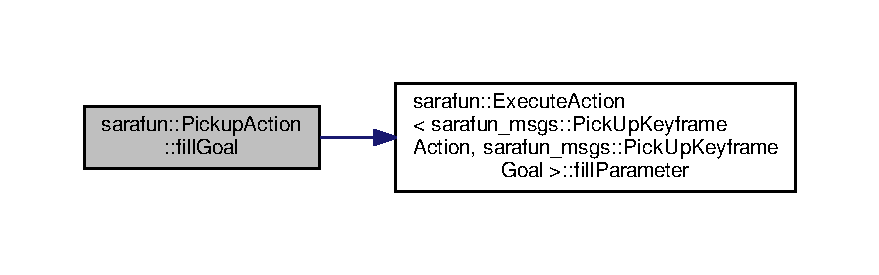
\includegraphics[width=350pt]{d8/dba/classsarafun_1_1PickupAction_a4aa9956733de9f12b52aa41038dbe87a_a4aa9956733de9f12b52aa41038dbe87a_cgraph}
\end{center}
\end{figure}


\hypertarget{classsarafun_1_1PickupAction_a02643cdc836095102e5622b660233f26_a02643cdc836095102e5622b660233f26}{\index{sarafun\-::\-Pickup\-Action@{sarafun\-::\-Pickup\-Action}!get\-Timeout\-Value@{get\-Timeout\-Value}}
\index{get\-Timeout\-Value@{get\-Timeout\-Value}!sarafun::PickupAction@{sarafun\-::\-Pickup\-Action}}
\subsubsection[{get\-Timeout\-Value}]{\setlength{\rightskip}{0pt plus 5cm}double sarafun\-::\-Pickup\-Action\-::get\-Timeout\-Value (
\begin{DoxyParamCaption}
{}
\end{DoxyParamCaption}
)\hspace{0.3cm}{\ttfamily [virtual]}}}\label{classsarafun_1_1PickupAction_a02643cdc836095102e5622b660233f26_a02643cdc836095102e5622b660233f26}
Provides the client with a timeout value for actionlib connections.

\begin{DoxyReturn}{Returns}
The timeout value (in seconds). 
\end{DoxyReturn}


Implements \hyperlink{classsarafun_1_1ExecuteAction_aba6cfa8a8ce19e735eb6394424df6d17_aba6cfa8a8ce19e735eb6394424df6d17}{sarafun\-::\-Execute\-Action$<$ sarafun\-\_\-msgs\-::\-Pick\-Up\-Keyframe\-Action, sarafun\-\_\-msgs\-::\-Pick\-Up\-Keyframe\-Goal $>$}.



Definition at line 13 of file Pickup\-Action.\-cpp.



References sarafun\-::\-Execute\-Action$<$ sarafun\-\_\-msgs\-::\-Pick\-Up\-Keyframe\-Action, sarafun\-\_\-msgs\-::\-Pick\-Up\-Keyframe\-Goal $>$\-::fill\-Parameter().



Here is the call graph for this function\-:
\nopagebreak
\begin{figure}[H]
\begin{center}
\leavevmode
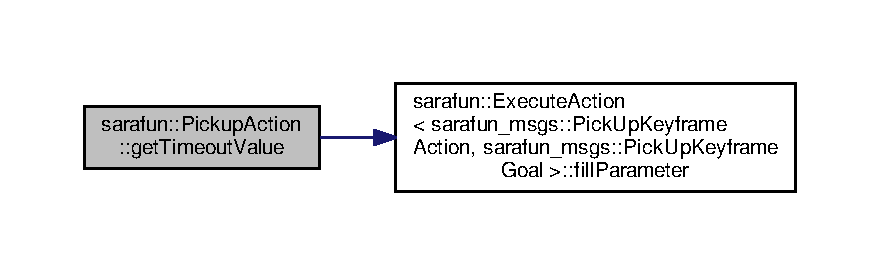
\includegraphics[width=350pt]{d8/dba/classsarafun_1_1PickupAction_a02643cdc836095102e5622b660233f26_a02643cdc836095102e5622b660233f26_cgraph}
\end{center}
\end{figure}




\subsection{Field Documentation}
\hypertarget{classsarafun_1_1PickupAction_a67b2fdfacb038bcd76dca5a3c2c2077c_a67b2fdfacb038bcd76dca5a3c2c2077c}{\index{sarafun\-::\-Pickup\-Action@{sarafun\-::\-Pickup\-Action}!bt\-\_\-name\-\_\-@{bt\-\_\-name\-\_\-}}
\index{bt\-\_\-name\-\_\-@{bt\-\_\-name\-\_\-}!sarafun::PickupAction@{sarafun\-::\-Pickup\-Action}}
\subsubsection[{bt\-\_\-name\-\_\-}]{\setlength{\rightskip}{0pt plus 5cm}std\-::string sarafun\-::\-Pickup\-Action\-::bt\-\_\-name\-\_\-\hspace{0.3cm}{\ttfamily [private]}}}\label{classsarafun_1_1PickupAction_a67b2fdfacb038bcd76dca5a3c2c2077c_a67b2fdfacb038bcd76dca5a3c2c2077c}


Definition at line 31 of file Pickup\-Action.\-h.

\hypertarget{classsarafun_1_1PickupAction_a7e7ccf1fed497576aebe7bb3c6cb57b3_a7e7ccf1fed497576aebe7bb3c6cb57b3}{\index{sarafun\-::\-Pickup\-Action@{sarafun\-::\-Pickup\-Action}!node\-\_\-handle\-\_\-@{node\-\_\-handle\-\_\-}}
\index{node\-\_\-handle\-\_\-@{node\-\_\-handle\-\_\-}!sarafun::PickupAction@{sarafun\-::\-Pickup\-Action}}
\subsubsection[{node\-\_\-handle\-\_\-}]{\setlength{\rightskip}{0pt plus 5cm}ros\-::\-Node\-Handle sarafun\-::\-Pickup\-Action\-::node\-\_\-handle\-\_\-\hspace{0.3cm}{\ttfamily [private]}}}\label{classsarafun_1_1PickupAction_a7e7ccf1fed497576aebe7bb3c6cb57b3_a7e7ccf1fed497576aebe7bb3c6cb57b3}


Definition at line 29 of file Pickup\-Action.\-h.



Referenced by Pickup\-Action().

\hypertarget{classsarafun_1_1PickupAction_a07fa3609628d2c5ac95a6cce904aa1b2_a07fa3609628d2c5ac95a6cce904aa1b2}{\index{sarafun\-::\-Pickup\-Action@{sarafun\-::\-Pickup\-Action}!node\-\_\-name\-\_\-@{node\-\_\-name\-\_\-}}
\index{node\-\_\-name\-\_\-@{node\-\_\-name\-\_\-}!sarafun::PickupAction@{sarafun\-::\-Pickup\-Action}}
\subsubsection[{node\-\_\-name\-\_\-}]{\setlength{\rightskip}{0pt plus 5cm}std\-::string sarafun\-::\-Pickup\-Action\-::node\-\_\-name\-\_\-\hspace{0.3cm}{\ttfamily [private]}}}\label{classsarafun_1_1PickupAction_a07fa3609628d2c5ac95a6cce904aa1b2_a07fa3609628d2c5ac95a6cce904aa1b2}


Definition at line 30 of file Pickup\-Action.\-h.



The documentation for this class was generated from the following files\-:\begin{DoxyCompactItemize}
\item 
Pickup\-Action.\-h\item 
Pickup\-Action.\-cpp\end{DoxyCompactItemize}

\hypertarget{classsarafun_1_1PlaceAction}{\section{sarafun\-:\-:Place\-Action Class Reference}
\label{classsarafun_1_1PlaceAction}\index{sarafun\-::\-Place\-Action@{sarafun\-::\-Place\-Action}}
}


{\ttfamily \#include $<$Place\-Action.\-h$>$}



Inheritance diagram for sarafun\-:\-:Place\-Action\-:
\nopagebreak
\begin{figure}[H]
\begin{center}
\leavevmode
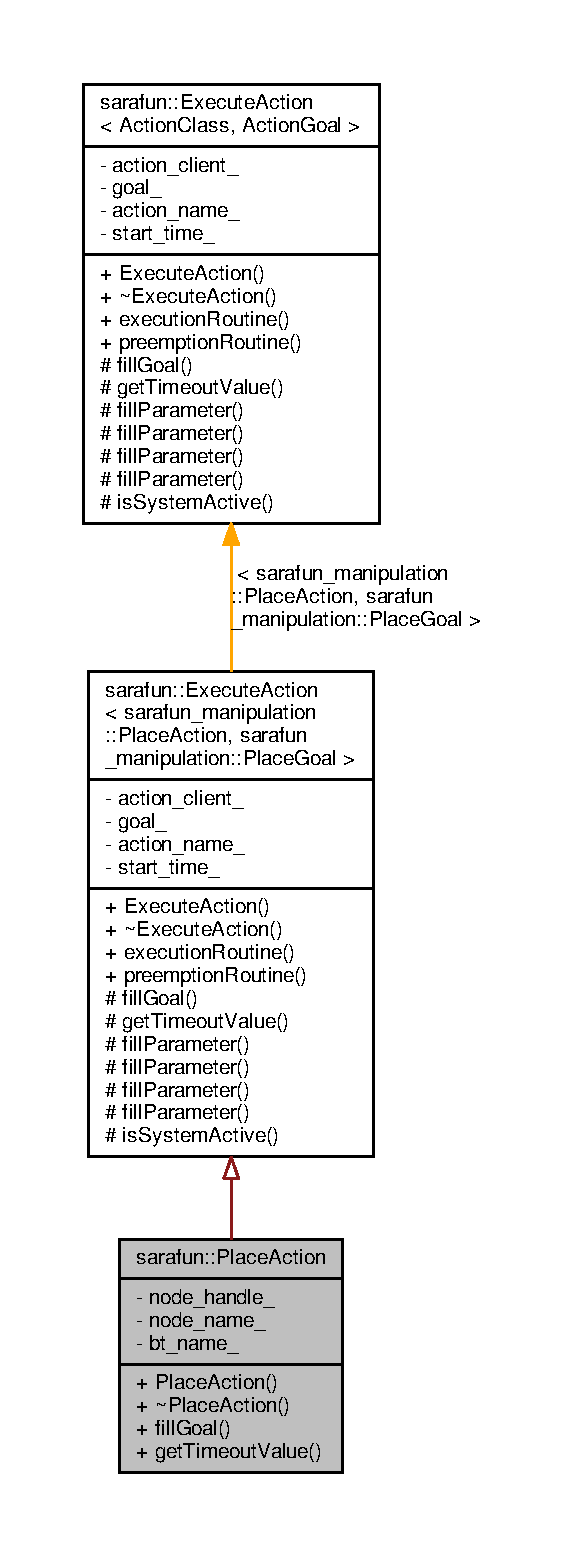
\includegraphics[height=550pt]{dd/d57/classsarafun_1_1PlaceAction__inherit__graph}
\end{center}
\end{figure}


Collaboration diagram for sarafun\-:\-:Place\-Action\-:
\nopagebreak
\begin{figure}[H]
\begin{center}
\leavevmode
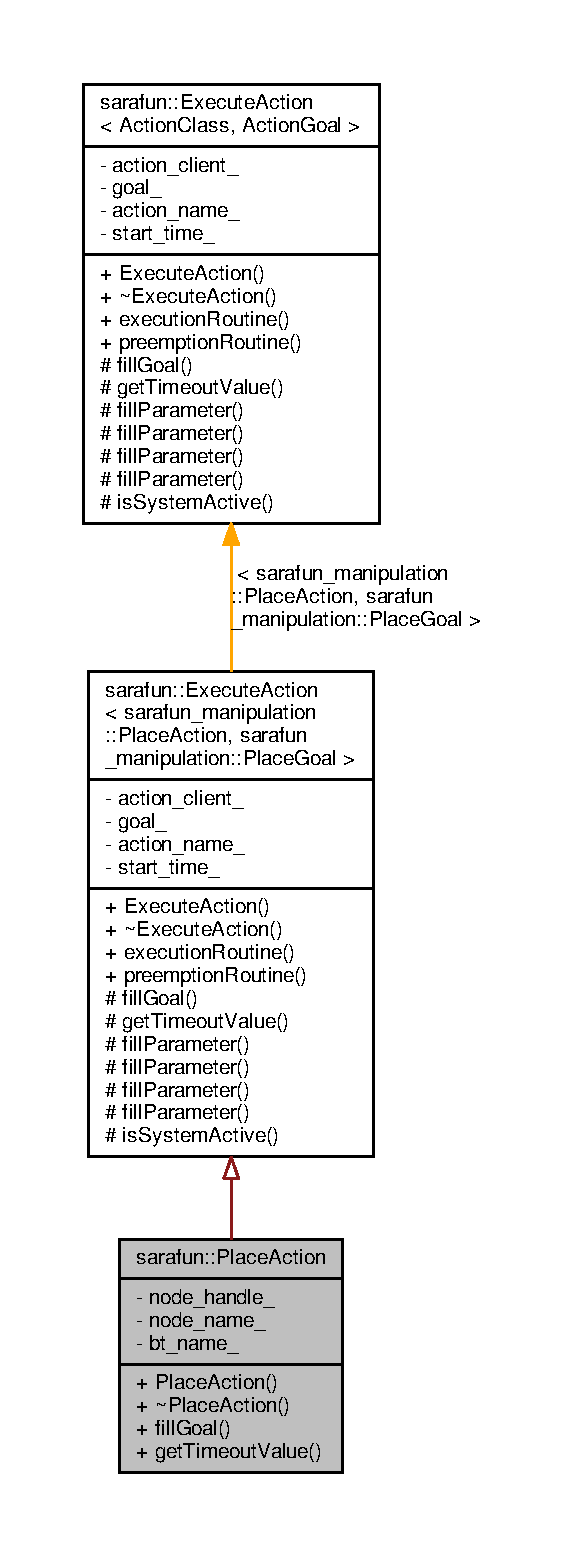
\includegraphics[height=550pt]{d9/df5/classsarafun_1_1PlaceAction__coll__graph}
\end{center}
\end{figure}
\subsection*{Public Member Functions}
\begin{DoxyCompactItemize}
\item 
\hyperlink{classsarafun_1_1PlaceAction_ad55f21266cf4807d831e2834fb6e5259_ad55f21266cf4807d831e2834fb6e5259}{Place\-Action} (std\-::string node\-\_\-name, std\-::string action\-\_\-name, std\-::string bt\-\_\-name)
\item 
\hyperlink{classsarafun_1_1PlaceAction_ae98d86339fdd0d275acff03c968ff834_ae98d86339fdd0d275acff03c968ff834}{$\sim$\-Place\-Action} ()
\item 
bool \hyperlink{classsarafun_1_1PlaceAction_a7d48e758adf6cea93fa15409bafda8c8_a7d48e758adf6cea93fa15409bafda8c8}{fill\-Goal} (sarafun\-\_\-manipulation\-::\-Place\-Goal \&goal)
\item 
double \hyperlink{classsarafun_1_1PlaceAction_a0b53372fd2de920c3ebd94c8c7f80b6a_a0b53372fd2de920c3ebd94c8c7f80b6a}{get\-Timeout\-Value} ()
\end{DoxyCompactItemize}
\subsection*{Private Attributes}
\begin{DoxyCompactItemize}
\item 
ros\-::\-Node\-Handle \hyperlink{classsarafun_1_1PlaceAction_a23f95c7612c9ebb2a64dcfa6ddbd9ec2_a23f95c7612c9ebb2a64dcfa6ddbd9ec2}{node\-\_\-handle\-\_\-}
\item 
std\-::string \hyperlink{classsarafun_1_1PlaceAction_ae8cc4bc053661bae5bdf93a08eaf3416_ae8cc4bc053661bae5bdf93a08eaf3416}{node\-\_\-name\-\_\-}
\item 
std\-::string \hyperlink{classsarafun_1_1PlaceAction_aa477ccd7678ea126e43f3a586be7d72d_aa477ccd7678ea126e43f3a586be7d72d}{bt\-\_\-name\-\_\-}
\end{DoxyCompactItemize}
\subsection*{Additional Inherited Members}


\subsection{Detailed Description}


Definition at line 9 of file Place\-Action.\-h.



\subsection{Constructor \& Destructor Documentation}
\hypertarget{classsarafun_1_1PlaceAction_ad55f21266cf4807d831e2834fb6e5259_ad55f21266cf4807d831e2834fb6e5259}{\index{sarafun\-::\-Place\-Action@{sarafun\-::\-Place\-Action}!Place\-Action@{Place\-Action}}
\index{Place\-Action@{Place\-Action}!sarafun::PlaceAction@{sarafun\-::\-Place\-Action}}
\subsubsection[{Place\-Action}]{\setlength{\rightskip}{0pt plus 5cm}sarafun\-::\-Place\-Action\-::\-Place\-Action (
\begin{DoxyParamCaption}
\item[{std\-::string}]{node\-\_\-name, }
\item[{std\-::string}]{action\-\_\-name, }
\item[{std\-::string}]{bt\-\_\-name}
\end{DoxyParamCaption}
)\hspace{0.3cm}{\ttfamily [inline]}}}\label{classsarafun_1_1PlaceAction_ad55f21266cf4807d831e2834fb6e5259_ad55f21266cf4807d831e2834fb6e5259}


Definition at line 12 of file Place\-Action.\-h.



References node\-\_\-handle\-\_\-.

\hypertarget{classsarafun_1_1PlaceAction_ae98d86339fdd0d275acff03c968ff834_ae98d86339fdd0d275acff03c968ff834}{\index{sarafun\-::\-Place\-Action@{sarafun\-::\-Place\-Action}!$\sim$\-Place\-Action@{$\sim$\-Place\-Action}}
\index{$\sim$\-Place\-Action@{$\sim$\-Place\-Action}!sarafun::PlaceAction@{sarafun\-::\-Place\-Action}}
\subsubsection[{$\sim$\-Place\-Action}]{\setlength{\rightskip}{0pt plus 5cm}sarafun\-::\-Place\-Action\-::$\sim$\-Place\-Action (
\begin{DoxyParamCaption}
{}
\end{DoxyParamCaption}
)\hspace{0.3cm}{\ttfamily [inline]}}}\label{classsarafun_1_1PlaceAction_ae98d86339fdd0d275acff03c968ff834_ae98d86339fdd0d275acff03c968ff834}


Definition at line 22 of file Place\-Action.\-h.



\subsection{Member Function Documentation}
\hypertarget{classsarafun_1_1PlaceAction_a7d48e758adf6cea93fa15409bafda8c8_a7d48e758adf6cea93fa15409bafda8c8}{\index{sarafun\-::\-Place\-Action@{sarafun\-::\-Place\-Action}!fill\-Goal@{fill\-Goal}}
\index{fill\-Goal@{fill\-Goal}!sarafun::PlaceAction@{sarafun\-::\-Place\-Action}}
\subsubsection[{fill\-Goal}]{\setlength{\rightskip}{0pt plus 5cm}bool sarafun\-::\-Place\-Action\-::fill\-Goal (
\begin{DoxyParamCaption}
\item[{sarafun\-\_\-manipulation\-::\-Place\-Goal \&}]{goal}
\end{DoxyParamCaption}
)\hspace{0.3cm}{\ttfamily [virtual]}}}\label{classsarafun_1_1PlaceAction_a7d48e758adf6cea93fa15409bafda8c8_a7d48e758adf6cea93fa15409bafda8c8}
Fills in the goal for a particular action.


\begin{DoxyParams}{Parameters}
{\em goal} & The actionlib goal message of the externally implemented action. \\
\hline
\end{DoxyParams}
\begin{DoxyReturn}{Returns}
False in case of error, true otherwise. 
\end{DoxyReturn}


Implements \hyperlink{classsarafun_1_1ExecuteAction_a6dd9c0f013d15a17d7e7ce8dbe40a436_a6dd9c0f013d15a17d7e7ce8dbe40a436}{sarafun\-::\-Execute\-Action$<$ sarafun\-\_\-manipulation\-::\-Place\-Action, sarafun\-\_\-manipulation\-::\-Place\-Goal $>$}.



Definition at line 11 of file Place\-Action.\-cpp.

\hypertarget{classsarafun_1_1PlaceAction_a0b53372fd2de920c3ebd94c8c7f80b6a_a0b53372fd2de920c3ebd94c8c7f80b6a}{\index{sarafun\-::\-Place\-Action@{sarafun\-::\-Place\-Action}!get\-Timeout\-Value@{get\-Timeout\-Value}}
\index{get\-Timeout\-Value@{get\-Timeout\-Value}!sarafun::PlaceAction@{sarafun\-::\-Place\-Action}}
\subsubsection[{get\-Timeout\-Value}]{\setlength{\rightskip}{0pt plus 5cm}double sarafun\-::\-Place\-Action\-::get\-Timeout\-Value (
\begin{DoxyParamCaption}
{}
\end{DoxyParamCaption}
)\hspace{0.3cm}{\ttfamily [virtual]}}}\label{classsarafun_1_1PlaceAction_a0b53372fd2de920c3ebd94c8c7f80b6a_a0b53372fd2de920c3ebd94c8c7f80b6a}
Provides the client with a timeout value for actionlib connections.

\begin{DoxyReturn}{Returns}
The timeout value (in seconds). 
\end{DoxyReturn}


Implements \hyperlink{classsarafun_1_1ExecuteAction_aba6cfa8a8ce19e735eb6394424df6d17_aba6cfa8a8ce19e735eb6394424df6d17}{sarafun\-::\-Execute\-Action$<$ sarafun\-\_\-manipulation\-::\-Place\-Action, sarafun\-\_\-manipulation\-::\-Place\-Goal $>$}.



Definition at line 4 of file Place\-Action.\-cpp.



References sarafun\-::\-Execute\-Action$<$ sarafun\-\_\-manipulation\-::\-Place\-Action, sarafun\-\_\-manipulation\-::\-Place\-Goal $>$\-::fill\-Parameter().



Here is the call graph for this function\-:
\nopagebreak
\begin{figure}[H]
\begin{center}
\leavevmode
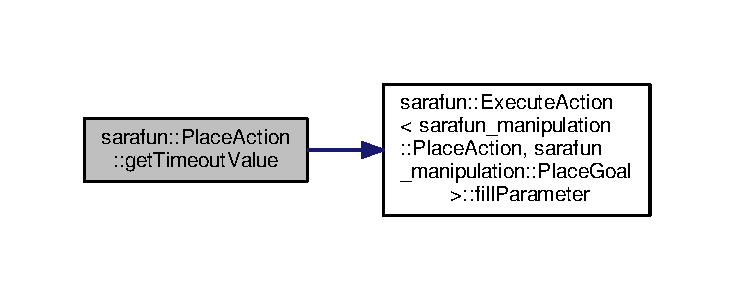
\includegraphics[width=350pt]{d3/dd9/classsarafun_1_1PlaceAction_a0b53372fd2de920c3ebd94c8c7f80b6a_a0b53372fd2de920c3ebd94c8c7f80b6a_cgraph}
\end{center}
\end{figure}




\subsection{Field Documentation}
\hypertarget{classsarafun_1_1PlaceAction_aa477ccd7678ea126e43f3a586be7d72d_aa477ccd7678ea126e43f3a586be7d72d}{\index{sarafun\-::\-Place\-Action@{sarafun\-::\-Place\-Action}!bt\-\_\-name\-\_\-@{bt\-\_\-name\-\_\-}}
\index{bt\-\_\-name\-\_\-@{bt\-\_\-name\-\_\-}!sarafun::PlaceAction@{sarafun\-::\-Place\-Action}}
\subsubsection[{bt\-\_\-name\-\_\-}]{\setlength{\rightskip}{0pt plus 5cm}std\-::string sarafun\-::\-Place\-Action\-::bt\-\_\-name\-\_\-\hspace{0.3cm}{\ttfamily [private]}}}\label{classsarafun_1_1PlaceAction_aa477ccd7678ea126e43f3a586be7d72d_aa477ccd7678ea126e43f3a586be7d72d}


Definition at line 30 of file Place\-Action.\-h.

\hypertarget{classsarafun_1_1PlaceAction_a23f95c7612c9ebb2a64dcfa6ddbd9ec2_a23f95c7612c9ebb2a64dcfa6ddbd9ec2}{\index{sarafun\-::\-Place\-Action@{sarafun\-::\-Place\-Action}!node\-\_\-handle\-\_\-@{node\-\_\-handle\-\_\-}}
\index{node\-\_\-handle\-\_\-@{node\-\_\-handle\-\_\-}!sarafun::PlaceAction@{sarafun\-::\-Place\-Action}}
\subsubsection[{node\-\_\-handle\-\_\-}]{\setlength{\rightskip}{0pt plus 5cm}ros\-::\-Node\-Handle sarafun\-::\-Place\-Action\-::node\-\_\-handle\-\_\-\hspace{0.3cm}{\ttfamily [private]}}}\label{classsarafun_1_1PlaceAction_a23f95c7612c9ebb2a64dcfa6ddbd9ec2_a23f95c7612c9ebb2a64dcfa6ddbd9ec2}


Definition at line 28 of file Place\-Action.\-h.



Referenced by Place\-Action().

\hypertarget{classsarafun_1_1PlaceAction_ae8cc4bc053661bae5bdf93a08eaf3416_ae8cc4bc053661bae5bdf93a08eaf3416}{\index{sarafun\-::\-Place\-Action@{sarafun\-::\-Place\-Action}!node\-\_\-name\-\_\-@{node\-\_\-name\-\_\-}}
\index{node\-\_\-name\-\_\-@{node\-\_\-name\-\_\-}!sarafun::PlaceAction@{sarafun\-::\-Place\-Action}}
\subsubsection[{node\-\_\-name\-\_\-}]{\setlength{\rightskip}{0pt plus 5cm}std\-::string sarafun\-::\-Place\-Action\-::node\-\_\-name\-\_\-\hspace{0.3cm}{\ttfamily [private]}}}\label{classsarafun_1_1PlaceAction_ae8cc4bc053661bae5bdf93a08eaf3416_ae8cc4bc053661bae5bdf93a08eaf3416}


Definition at line 29 of file Place\-Action.\-h.



The documentation for this class was generated from the following files\-:\begin{DoxyCompactItemize}
\item 
Place\-Action.\-h\item 
Place\-Action.\-cpp\end{DoxyCompactItemize}

\hypertarget{classsarafun_1_1RetractAction}{\section{sarafun\-:\-:Retract\-Action Class Reference}
\label{classsarafun_1_1RetractAction}\index{sarafun\-::\-Retract\-Action@{sarafun\-::\-Retract\-Action}}
}


{\ttfamily \#include $<$Retract\-Action.\-h$>$}



Inheritance diagram for sarafun\-:\-:Retract\-Action\-:\nopagebreak
\begin{figure}[H]
\begin{center}
\leavevmode
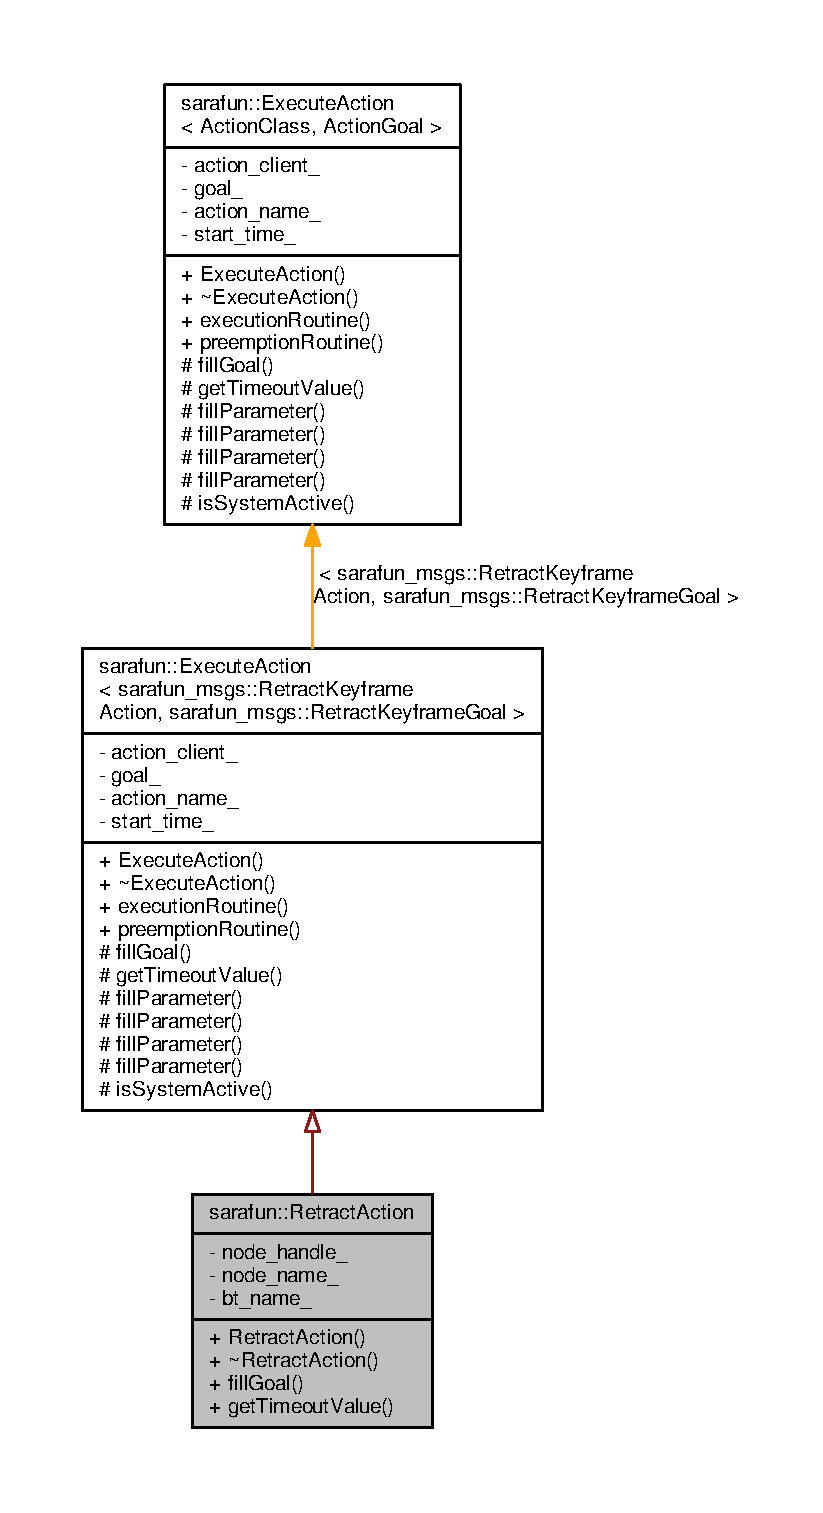
\includegraphics[height=550pt]{d6/d3a/classsarafun_1_1RetractAction__inherit__graph}
\end{center}
\end{figure}


Collaboration diagram for sarafun\-:\-:Retract\-Action\-:\nopagebreak
\begin{figure}[H]
\begin{center}
\leavevmode
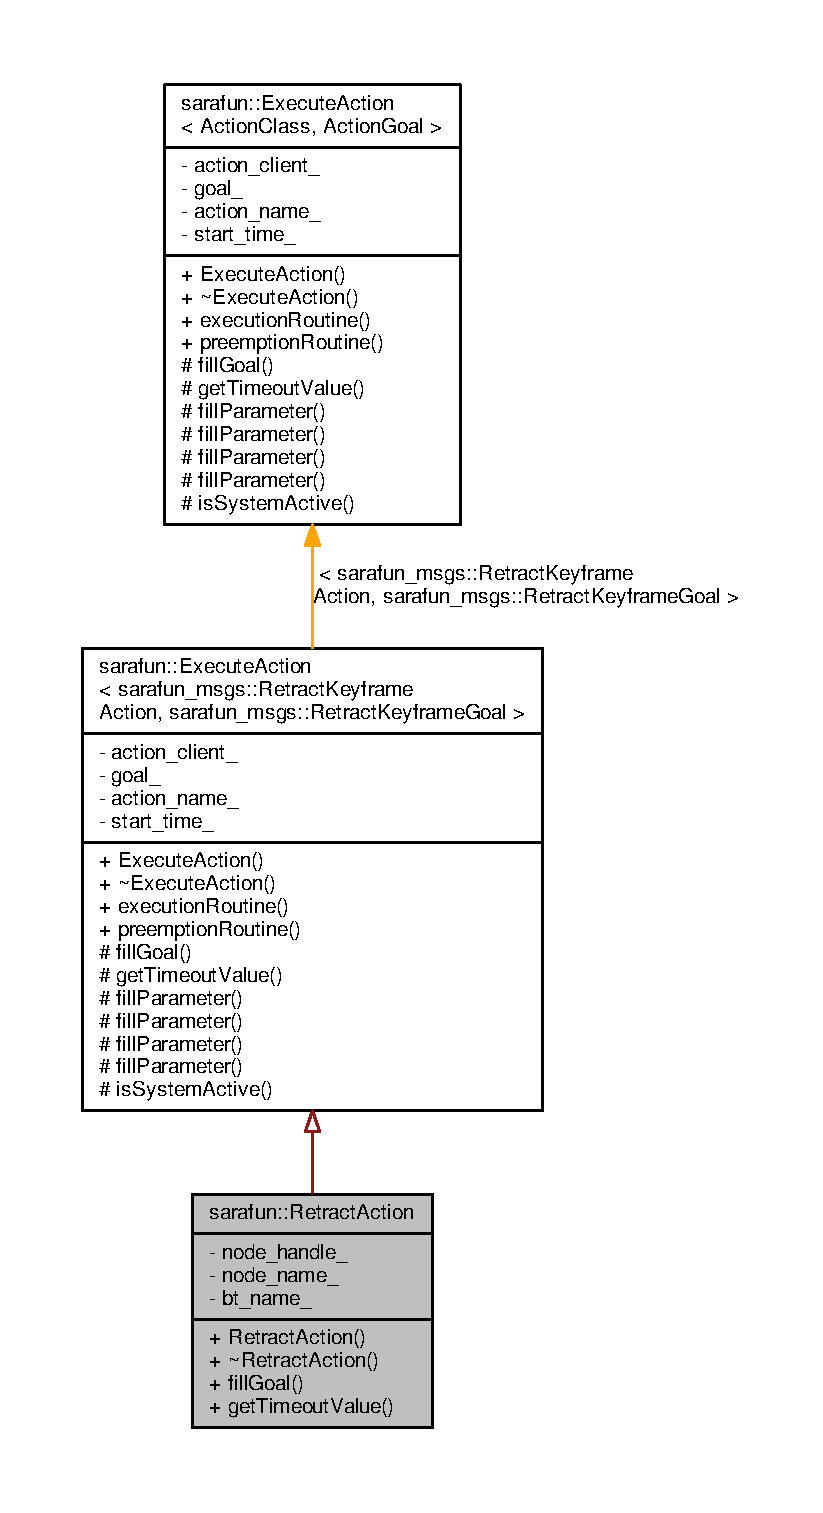
\includegraphics[height=550pt]{de/d4f/classsarafun_1_1RetractAction__coll__graph}
\end{center}
\end{figure}
\subsection*{Public Member Functions}
\begin{DoxyCompactItemize}
\item 
\hyperlink{classsarafun_1_1RetractAction_a0f56a3d5ff6c07f48bbd3cede93f0a81_a0f56a3d5ff6c07f48bbd3cede93f0a81}{Retract\-Action} (std\-::string node\-\_\-name, std\-::string action\-\_\-name, std\-::string bt\-\_\-name)
\item 
\hyperlink{classsarafun_1_1RetractAction_adb37a0fb90d06636009f90b7565f00cf_adb37a0fb90d06636009f90b7565f00cf}{$\sim$\-Retract\-Action} ()
\item 
bool \hyperlink{classsarafun_1_1RetractAction_ad0db1c2615d68603bc972ffa26049a70_ad0db1c2615d68603bc972ffa26049a70}{fill\-Goal} (sarafun\-\_\-msgs\-::\-Retract\-Keyframe\-Goal \&goal)
\item 
double \hyperlink{classsarafun_1_1RetractAction_af95bb8d3826dbe1444a8a3e12d8596b0_af95bb8d3826dbe1444a8a3e12d8596b0}{get\-Timeout\-Value} ()
\end{DoxyCompactItemize}
\subsection*{Private Attributes}
\begin{DoxyCompactItemize}
\item 
ros\-::\-Node\-Handle \hyperlink{classsarafun_1_1RetractAction_aaed00694d79d51ddd40fa3d098faaccd_aaed00694d79d51ddd40fa3d098faaccd}{node\-\_\-handle\-\_\-}
\item 
std\-::string \hyperlink{classsarafun_1_1RetractAction_ab4386c388115f5b76ff82f55895cc1ee_ab4386c388115f5b76ff82f55895cc1ee}{node\-\_\-name\-\_\-}
\item 
std\-::string \hyperlink{classsarafun_1_1RetractAction_a186b48e8f63ea5e0cd8c8047cfa36843_a186b48e8f63ea5e0cd8c8047cfa36843}{bt\-\_\-name\-\_\-}
\end{DoxyCompactItemize}
\subsection*{Additional Inherited Members}


\subsection{Detailed Description}


Definition at line 9 of file Retract\-Action.\-h.



\subsection{Constructor \& Destructor Documentation}
\hypertarget{classsarafun_1_1RetractAction_a0f56a3d5ff6c07f48bbd3cede93f0a81_a0f56a3d5ff6c07f48bbd3cede93f0a81}{\index{sarafun\-::\-Retract\-Action@{sarafun\-::\-Retract\-Action}!Retract\-Action@{Retract\-Action}}
\index{Retract\-Action@{Retract\-Action}!sarafun::RetractAction@{sarafun\-::\-Retract\-Action}}
\subsubsection[{Retract\-Action}]{\setlength{\rightskip}{0pt plus 5cm}sarafun\-::\-Retract\-Action\-::\-Retract\-Action (
\begin{DoxyParamCaption}
\item[{std\-::string}]{node\-\_\-name, }
\item[{std\-::string}]{action\-\_\-name, }
\item[{std\-::string}]{bt\-\_\-name}
\end{DoxyParamCaption}
)\hspace{0.3cm}{\ttfamily [inline]}}}\label{classsarafun_1_1RetractAction_a0f56a3d5ff6c07f48bbd3cede93f0a81_a0f56a3d5ff6c07f48bbd3cede93f0a81}


Definition at line 13 of file Retract\-Action.\-h.



References node\-\_\-handle\-\_\-.

\hypertarget{classsarafun_1_1RetractAction_adb37a0fb90d06636009f90b7565f00cf_adb37a0fb90d06636009f90b7565f00cf}{\index{sarafun\-::\-Retract\-Action@{sarafun\-::\-Retract\-Action}!$\sim$\-Retract\-Action@{$\sim$\-Retract\-Action}}
\index{$\sim$\-Retract\-Action@{$\sim$\-Retract\-Action}!sarafun::RetractAction@{sarafun\-::\-Retract\-Action}}
\subsubsection[{$\sim$\-Retract\-Action}]{\setlength{\rightskip}{0pt plus 5cm}sarafun\-::\-Retract\-Action\-::$\sim$\-Retract\-Action (
\begin{DoxyParamCaption}
{}
\end{DoxyParamCaption}
)\hspace{0.3cm}{\ttfamily [inline]}}}\label{classsarafun_1_1RetractAction_adb37a0fb90d06636009f90b7565f00cf_adb37a0fb90d06636009f90b7565f00cf}


Definition at line 23 of file Retract\-Action.\-h.



\subsection{Member Function Documentation}
\hypertarget{classsarafun_1_1RetractAction_ad0db1c2615d68603bc972ffa26049a70_ad0db1c2615d68603bc972ffa26049a70}{\index{sarafun\-::\-Retract\-Action@{sarafun\-::\-Retract\-Action}!fill\-Goal@{fill\-Goal}}
\index{fill\-Goal@{fill\-Goal}!sarafun::RetractAction@{sarafun\-::\-Retract\-Action}}
\subsubsection[{fill\-Goal}]{\setlength{\rightskip}{0pt plus 5cm}bool sarafun\-::\-Retract\-Action\-::fill\-Goal (
\begin{DoxyParamCaption}
\item[{sarafun\-\_\-msgs\-::\-Retract\-Keyframe\-Goal \&}]{goal}
\end{DoxyParamCaption}
)\hspace{0.3cm}{\ttfamily [virtual]}}}\label{classsarafun_1_1RetractAction_ad0db1c2615d68603bc972ffa26049a70_ad0db1c2615d68603bc972ffa26049a70}
Fills in the goal for a particular action.


\begin{DoxyParams}{Parameters}
{\em goal} & The actionlib goal message of the externally implemented action. \\
\hline
\end{DoxyParams}
\begin{DoxyReturn}{Returns}
False in case of error, true otherwise. 
\end{DoxyReturn}


Implements \hyperlink{classsarafun_1_1ExecuteAction_a6dd9c0f013d15a17d7e7ce8dbe40a436_a6dd9c0f013d15a17d7e7ce8dbe40a436}{sarafun\-::\-Execute\-Action$<$ sarafun\-\_\-msgs\-::\-Retract\-Keyframe\-Action, sarafun\-\_\-msgs\-::\-Retract\-Keyframe\-Goal $>$}.



Definition at line 4 of file Retract\-Action.\-cpp.



References sarafun\-::\-Execute\-Action$<$ sarafun\-\_\-msgs\-::\-Retract\-Keyframe\-Action, sarafun\-\_\-msgs\-::\-Retract\-Keyframe\-Goal $>$\-::fill\-Parameter().



Here is the call graph for this function\-:\nopagebreak
\begin{figure}[H]
\begin{center}
\leavevmode
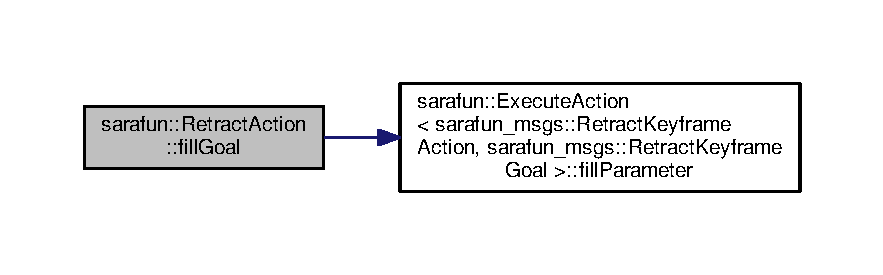
\includegraphics[width=350pt]{d4/dd3/classsarafun_1_1RetractAction_ad0db1c2615d68603bc972ffa26049a70_ad0db1c2615d68603bc972ffa26049a70_cgraph}
\end{center}
\end{figure}


\hypertarget{classsarafun_1_1RetractAction_af95bb8d3826dbe1444a8a3e12d8596b0_af95bb8d3826dbe1444a8a3e12d8596b0}{\index{sarafun\-::\-Retract\-Action@{sarafun\-::\-Retract\-Action}!get\-Timeout\-Value@{get\-Timeout\-Value}}
\index{get\-Timeout\-Value@{get\-Timeout\-Value}!sarafun::RetractAction@{sarafun\-::\-Retract\-Action}}
\subsubsection[{get\-Timeout\-Value}]{\setlength{\rightskip}{0pt plus 5cm}double sarafun\-::\-Retract\-Action\-::get\-Timeout\-Value (
\begin{DoxyParamCaption}
{}
\end{DoxyParamCaption}
)\hspace{0.3cm}{\ttfamily [virtual]}}}\label{classsarafun_1_1RetractAction_af95bb8d3826dbe1444a8a3e12d8596b0_af95bb8d3826dbe1444a8a3e12d8596b0}
Provides the client with a timeout value for actionlib connections.

\begin{DoxyReturn}{Returns}
The timeout value (in seconds). 
\end{DoxyReturn}


Implements \hyperlink{classsarafun_1_1ExecuteAction_aba6cfa8a8ce19e735eb6394424df6d17_aba6cfa8a8ce19e735eb6394424df6d17}{sarafun\-::\-Execute\-Action$<$ sarafun\-\_\-msgs\-::\-Retract\-Keyframe\-Action, sarafun\-\_\-msgs\-::\-Retract\-Keyframe\-Goal $>$}.



Definition at line 13 of file Retract\-Action.\-cpp.



References sarafun\-::\-Execute\-Action$<$ sarafun\-\_\-msgs\-::\-Retract\-Keyframe\-Action, sarafun\-\_\-msgs\-::\-Retract\-Keyframe\-Goal $>$\-::fill\-Parameter().



Here is the call graph for this function\-:\nopagebreak
\begin{figure}[H]
\begin{center}
\leavevmode
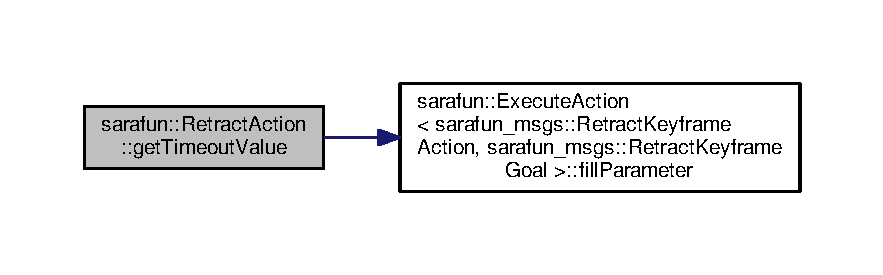
\includegraphics[width=350pt]{d4/dd3/classsarafun_1_1RetractAction_af95bb8d3826dbe1444a8a3e12d8596b0_af95bb8d3826dbe1444a8a3e12d8596b0_cgraph}
\end{center}
\end{figure}




\subsection{Field Documentation}
\hypertarget{classsarafun_1_1RetractAction_a186b48e8f63ea5e0cd8c8047cfa36843_a186b48e8f63ea5e0cd8c8047cfa36843}{\index{sarafun\-::\-Retract\-Action@{sarafun\-::\-Retract\-Action}!bt\-\_\-name\-\_\-@{bt\-\_\-name\-\_\-}}
\index{bt\-\_\-name\-\_\-@{bt\-\_\-name\-\_\-}!sarafun::RetractAction@{sarafun\-::\-Retract\-Action}}
\subsubsection[{bt\-\_\-name\-\_\-}]{\setlength{\rightskip}{0pt plus 5cm}std\-::string sarafun\-::\-Retract\-Action\-::bt\-\_\-name\-\_\-\hspace{0.3cm}{\ttfamily [private]}}}\label{classsarafun_1_1RetractAction_a186b48e8f63ea5e0cd8c8047cfa36843_a186b48e8f63ea5e0cd8c8047cfa36843}


Definition at line 31 of file Retract\-Action.\-h.

\hypertarget{classsarafun_1_1RetractAction_aaed00694d79d51ddd40fa3d098faaccd_aaed00694d79d51ddd40fa3d098faaccd}{\index{sarafun\-::\-Retract\-Action@{sarafun\-::\-Retract\-Action}!node\-\_\-handle\-\_\-@{node\-\_\-handle\-\_\-}}
\index{node\-\_\-handle\-\_\-@{node\-\_\-handle\-\_\-}!sarafun::RetractAction@{sarafun\-::\-Retract\-Action}}
\subsubsection[{node\-\_\-handle\-\_\-}]{\setlength{\rightskip}{0pt plus 5cm}ros\-::\-Node\-Handle sarafun\-::\-Retract\-Action\-::node\-\_\-handle\-\_\-\hspace{0.3cm}{\ttfamily [private]}}}\label{classsarafun_1_1RetractAction_aaed00694d79d51ddd40fa3d098faaccd_aaed00694d79d51ddd40fa3d098faaccd}


Definition at line 29 of file Retract\-Action.\-h.



Referenced by Retract\-Action().

\hypertarget{classsarafun_1_1RetractAction_ab4386c388115f5b76ff82f55895cc1ee_ab4386c388115f5b76ff82f55895cc1ee}{\index{sarafun\-::\-Retract\-Action@{sarafun\-::\-Retract\-Action}!node\-\_\-name\-\_\-@{node\-\_\-name\-\_\-}}
\index{node\-\_\-name\-\_\-@{node\-\_\-name\-\_\-}!sarafun::RetractAction@{sarafun\-::\-Retract\-Action}}
\subsubsection[{node\-\_\-name\-\_\-}]{\setlength{\rightskip}{0pt plus 5cm}std\-::string sarafun\-::\-Retract\-Action\-::node\-\_\-name\-\_\-\hspace{0.3cm}{\ttfamily [private]}}}\label{classsarafun_1_1RetractAction_ab4386c388115f5b76ff82f55895cc1ee_ab4386c388115f5b76ff82f55895cc1ee}


Definition at line 30 of file Retract\-Action.\-h.



The documentation for this class was generated from the following files\-:\begin{DoxyCompactItemize}
\item 
Retract\-Action.\-h\item 
Retract\-Action.\-cpp\end{DoxyCompactItemize}

\hypertarget{classtree__generator_1_1SubTreeFromKF}{\section{tree\-\_\-generator\-:\-:Sub\-Tree\-From\-K\-F Class Reference}
\label{classtree__generator_1_1SubTreeFromKF}\index{tree\-\_\-generator\-::\-Sub\-Tree\-From\-K\-F@{tree\-\_\-generator\-::\-Sub\-Tree\-From\-K\-F}}
}


{\ttfamily \#include $<$Tree\-From\-K\-F.\-hpp$>$}



Collaboration diagram for tree\-\_\-generator\-:\-:Sub\-Tree\-From\-K\-F\-:
\nopagebreak
\begin{figure}[H]
\begin{center}
\leavevmode
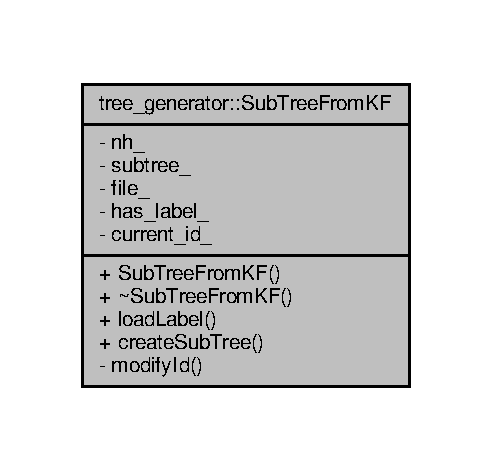
\includegraphics[width=236pt]{de/d5a/classtree__generator_1_1SubTreeFromKF__coll__graph}
\end{center}
\end{figure}
\subsection*{Public Member Functions}
\begin{DoxyCompactItemize}
\item 
\hyperlink{classtree__generator_1_1SubTreeFromKF_ab7af1f33766b79ffb8d596db12a567f4_ab7af1f33766b79ffb8d596db12a567f4}{Sub\-Tree\-From\-K\-F} ()
\item 
\hyperlink{classtree__generator_1_1SubTreeFromKF_aa6f44a5c131577ea1719a3fa3a28d65d_aa6f44a5c131577ea1719a3fa3a28d65d}{$\sim$\-Sub\-Tree\-From\-K\-F} ()
\item 
bool \hyperlink{classtree__generator_1_1SubTreeFromKF_a3e4e089333af3305e40434e49dcc0878_a3e4e089333af3305e40434e49dcc0878}{load\-Label} (std\-::string label)
\item 
json \hyperlink{classtree__generator_1_1SubTreeFromKF_a531cc034d2af6a380a40763894542760_a531cc034d2af6a380a40763894542760}{create\-Sub\-Tree} (std\-::vector$<$ int $>$ \&indices)
\end{DoxyCompactItemize}
\subsection*{Private Member Functions}
\begin{DoxyCompactItemize}
\item 
json \hyperlink{classtree__generator_1_1SubTreeFromKF_aea29705cc665f48d15ee436a409d55a9_aea29705cc665f48d15ee436a409d55a9}{modify\-Id} (json node, std\-::vector$<$ int $>$ \&indices)
\end{DoxyCompactItemize}
\subsection*{Private Attributes}
\begin{DoxyCompactItemize}
\item 
ros\-::\-Node\-Handle \hyperlink{classtree__generator_1_1SubTreeFromKF_af32fafef64d1f98df5b38697d1984d80_af32fafef64d1f98df5b38697d1984d80}{nh\-\_\-}
\item 
json \hyperlink{classtree__generator_1_1SubTreeFromKF_a2c9edbe4a6243a1a8bad6ae524df884b_a2c9edbe4a6243a1a8bad6ae524df884b}{subtree\-\_\-}
\item 
std\-::ifstream \hyperlink{classtree__generator_1_1SubTreeFromKF_a66c16669fa438a7a923a88557f8c9654_a66c16669fa438a7a923a88557f8c9654}{file\-\_\-}
\item 
bool \hyperlink{classtree__generator_1_1SubTreeFromKF_abf3280300d7972d36344adf0196d6aba_abf3280300d7972d36344adf0196d6aba}{has\-\_\-label\-\_\-}
\item 
std\-::string \hyperlink{classtree__generator_1_1SubTreeFromKF_a93cab044cd81910fd6b22522e7aa12a6_a93cab044cd81910fd6b22522e7aa12a6}{current\-\_\-id\-\_\-}
\end{DoxyCompactItemize}


\subsection{Detailed Description}
This class constructs one pre-\/defined B\-T subtree, given the semantic information contained in a keyframe.

The files describing the subtrees are defined in the /data/subtrees directory, and must have names matching the labels loaded in the parameter server. 

Definition at line 22 of file Tree\-From\-K\-F.\-hpp.



\subsection{Constructor \& Destructor Documentation}
\hypertarget{classtree__generator_1_1SubTreeFromKF_ab7af1f33766b79ffb8d596db12a567f4_ab7af1f33766b79ffb8d596db12a567f4}{\index{tree\-\_\-generator\-::\-Sub\-Tree\-From\-K\-F@{tree\-\_\-generator\-::\-Sub\-Tree\-From\-K\-F}!Sub\-Tree\-From\-K\-F@{Sub\-Tree\-From\-K\-F}}
\index{Sub\-Tree\-From\-K\-F@{Sub\-Tree\-From\-K\-F}!tree_generator::SubTreeFromKF@{tree\-\_\-generator\-::\-Sub\-Tree\-From\-K\-F}}
\subsubsection[{Sub\-Tree\-From\-K\-F}]{\setlength{\rightskip}{0pt plus 5cm}tree\-\_\-generator\-::\-Sub\-Tree\-From\-K\-F\-::\-Sub\-Tree\-From\-K\-F (
\begin{DoxyParamCaption}
{}
\end{DoxyParamCaption}
)}}\label{classtree__generator_1_1SubTreeFromKF_ab7af1f33766b79ffb8d596db12a567f4_ab7af1f33766b79ffb8d596db12a567f4}


Definition at line 6 of file Tree\-From\-K\-F.\-cpp.



References has\-\_\-label\-\_\-, and nh\-\_\-.

\hypertarget{classtree__generator_1_1SubTreeFromKF_aa6f44a5c131577ea1719a3fa3a28d65d_aa6f44a5c131577ea1719a3fa3a28d65d}{\index{tree\-\_\-generator\-::\-Sub\-Tree\-From\-K\-F@{tree\-\_\-generator\-::\-Sub\-Tree\-From\-K\-F}!$\sim$\-Sub\-Tree\-From\-K\-F@{$\sim$\-Sub\-Tree\-From\-K\-F}}
\index{$\sim$\-Sub\-Tree\-From\-K\-F@{$\sim$\-Sub\-Tree\-From\-K\-F}!tree_generator::SubTreeFromKF@{tree\-\_\-generator\-::\-Sub\-Tree\-From\-K\-F}}
\subsubsection[{$\sim$\-Sub\-Tree\-From\-K\-F}]{\setlength{\rightskip}{0pt plus 5cm}tree\-\_\-generator\-::\-Sub\-Tree\-From\-K\-F\-::$\sim$\-Sub\-Tree\-From\-K\-F (
\begin{DoxyParamCaption}
{}
\end{DoxyParamCaption}
)\hspace{0.3cm}{\ttfamily [inline]}}}\label{classtree__generator_1_1SubTreeFromKF_aa6f44a5c131577ea1719a3fa3a28d65d_aa6f44a5c131577ea1719a3fa3a28d65d}


Definition at line 25 of file Tree\-From\-K\-F.\-hpp.



\subsection{Member Function Documentation}
\hypertarget{classtree__generator_1_1SubTreeFromKF_a531cc034d2af6a380a40763894542760_a531cc034d2af6a380a40763894542760}{\index{tree\-\_\-generator\-::\-Sub\-Tree\-From\-K\-F@{tree\-\_\-generator\-::\-Sub\-Tree\-From\-K\-F}!create\-Sub\-Tree@{create\-Sub\-Tree}}
\index{create\-Sub\-Tree@{create\-Sub\-Tree}!tree_generator::SubTreeFromKF@{tree\-\_\-generator\-::\-Sub\-Tree\-From\-K\-F}}
\subsubsection[{create\-Sub\-Tree}]{\setlength{\rightskip}{0pt plus 5cm}json tree\-\_\-generator\-::\-Sub\-Tree\-From\-K\-F\-::create\-Sub\-Tree (
\begin{DoxyParamCaption}
\item[{std\-::vector$<$ int $>$ \&}]{indices}
\end{DoxyParamCaption}
)}}\label{classtree__generator_1_1SubTreeFromKF_a531cc034d2af6a380a40763894542760_a531cc034d2af6a380a40763894542760}


Definition at line 53 of file Tree\-From\-K\-F.\-cpp.



References file\-\_\-, has\-\_\-label\-\_\-, modify\-Id(), and subtree\-\_\-.



Referenced by tree\-\_\-generator\-::\-Tree\-From\-K\-F\-::create\-Tree().



Here is the call graph for this function\-:
\nopagebreak
\begin{figure}[H]
\begin{center}
\leavevmode
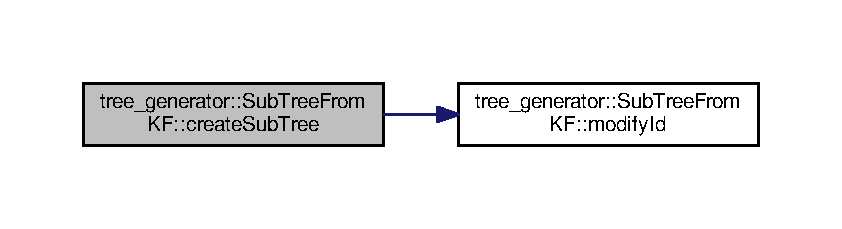
\includegraphics[width=350pt]{d9/de6/classtree__generator_1_1SubTreeFromKF_a531cc034d2af6a380a40763894542760_a531cc034d2af6a380a40763894542760_cgraph}
\end{center}
\end{figure}


\hypertarget{classtree__generator_1_1SubTreeFromKF_a3e4e089333af3305e40434e49dcc0878_a3e4e089333af3305e40434e49dcc0878}{\index{tree\-\_\-generator\-::\-Sub\-Tree\-From\-K\-F@{tree\-\_\-generator\-::\-Sub\-Tree\-From\-K\-F}!load\-Label@{load\-Label}}
\index{load\-Label@{load\-Label}!tree_generator::SubTreeFromKF@{tree\-\_\-generator\-::\-Sub\-Tree\-From\-K\-F}}
\subsubsection[{load\-Label}]{\setlength{\rightskip}{0pt plus 5cm}bool tree\-\_\-generator\-::\-Sub\-Tree\-From\-K\-F\-::load\-Label (
\begin{DoxyParamCaption}
\item[{std\-::string}]{label}
\end{DoxyParamCaption}
)}}\label{classtree__generator_1_1SubTreeFromKF_a3e4e089333af3305e40434e49dcc0878_a3e4e089333af3305e40434e49dcc0878}
Recovers a B\-T subtree with a label that matches the keyframe.


\begin{DoxyParams}{Parameters}
{\em label} & The K\-F label that identifies the subtree. \\
\hline
\end{DoxyParams}
\begin{DoxyReturn}{Returns}
True in case the label exists and the file is recovered. False otherwise. 
\end{DoxyReturn}


Definition at line 26 of file Tree\-From\-K\-F.\-cpp.



References file\-\_\-, has\-\_\-label\-\_\-, nh\-\_\-, and tree\-\_\-generator\-::replace\-With\-Underscore().



Referenced by tree\-\_\-generator\-::\-Tree\-From\-K\-F\-::create\-Tree().



Here is the call graph for this function\-:
\nopagebreak
\begin{figure}[H]
\begin{center}
\leavevmode
\includegraphics[width=350pt]{d9/de6/classtree__generator_1_1SubTreeFromKF_a3e4e089333af3305e40434e49dcc0878_a3e4e089333af3305e40434e49dcc0878_cgraph}
\end{center}
\end{figure}


\hypertarget{classtree__generator_1_1SubTreeFromKF_aea29705cc665f48d15ee436a409d55a9_aea29705cc665f48d15ee436a409d55a9}{\index{tree\-\_\-generator\-::\-Sub\-Tree\-From\-K\-F@{tree\-\_\-generator\-::\-Sub\-Tree\-From\-K\-F}!modify\-Id@{modify\-Id}}
\index{modify\-Id@{modify\-Id}!tree_generator::SubTreeFromKF@{tree\-\_\-generator\-::\-Sub\-Tree\-From\-K\-F}}
\subsubsection[{modify\-Id}]{\setlength{\rightskip}{0pt plus 5cm}json tree\-\_\-generator\-::\-Sub\-Tree\-From\-K\-F\-::modify\-Id (
\begin{DoxyParamCaption}
\item[{json}]{node, }
\item[{std\-::vector$<$ int $>$ \&}]{indices}
\end{DoxyParamCaption}
)\hspace{0.3cm}{\ttfamily [private]}}}\label{classtree__generator_1_1SubTreeFromKF_aea29705cc665f48d15ee436a409d55a9_aea29705cc665f48d15ee436a409d55a9}
Make sure that the created json subtree has nodes with proper indices.


\begin{DoxyParams}{Parameters}
{\em node} & The J\-S\-O\-N node with the subtree description. \\
\hline
{\em indices} & The vector of indices. \\
\hline
\end{DoxyParams}
\begin{DoxyReturn}{Returns}
The modified json N\-O\-D\-E. 
\end{DoxyReturn}

\begin{DoxyExceptions}{Exceptions}
{\em logic\-\_\-error} & \\
\hline
\end{DoxyExceptions}


Definition at line 77 of file Tree\-From\-K\-F.\-cpp.



References tree\-\_\-generator\-::\-A\-C\-T\-I\-O\-N, tree\-\_\-generator\-::\-C\-O\-N\-D\-I\-T\-I\-O\-N, tree\-\_\-generator\-::\-S\-E\-L, tree\-\_\-generator\-::\-S\-E\-L\-S\-T\-A\-R, tree\-\_\-generator\-::\-S\-E\-Q, and tree\-\_\-generator\-::\-S\-E\-Q\-S\-T\-A\-R.



Referenced by create\-Sub\-Tree().



\subsection{Field Documentation}
\hypertarget{classtree__generator_1_1SubTreeFromKF_a93cab044cd81910fd6b22522e7aa12a6_a93cab044cd81910fd6b22522e7aa12a6}{\index{tree\-\_\-generator\-::\-Sub\-Tree\-From\-K\-F@{tree\-\_\-generator\-::\-Sub\-Tree\-From\-K\-F}!current\-\_\-id\-\_\-@{current\-\_\-id\-\_\-}}
\index{current\-\_\-id\-\_\-@{current\-\_\-id\-\_\-}!tree_generator::SubTreeFromKF@{tree\-\_\-generator\-::\-Sub\-Tree\-From\-K\-F}}
\subsubsection[{current\-\_\-id\-\_\-}]{\setlength{\rightskip}{0pt plus 5cm}std\-::string tree\-\_\-generator\-::\-Sub\-Tree\-From\-K\-F\-::current\-\_\-id\-\_\-\hspace{0.3cm}{\ttfamily [private]}}}\label{classtree__generator_1_1SubTreeFromKF_a93cab044cd81910fd6b22522e7aa12a6_a93cab044cd81910fd6b22522e7aa12a6}


Definition at line 52 of file Tree\-From\-K\-F.\-hpp.

\hypertarget{classtree__generator_1_1SubTreeFromKF_a66c16669fa438a7a923a88557f8c9654_a66c16669fa438a7a923a88557f8c9654}{\index{tree\-\_\-generator\-::\-Sub\-Tree\-From\-K\-F@{tree\-\_\-generator\-::\-Sub\-Tree\-From\-K\-F}!file\-\_\-@{file\-\_\-}}
\index{file\-\_\-@{file\-\_\-}!tree_generator::SubTreeFromKF@{tree\-\_\-generator\-::\-Sub\-Tree\-From\-K\-F}}
\subsubsection[{file\-\_\-}]{\setlength{\rightskip}{0pt plus 5cm}std\-::ifstream tree\-\_\-generator\-::\-Sub\-Tree\-From\-K\-F\-::file\-\_\-\hspace{0.3cm}{\ttfamily [private]}}}\label{classtree__generator_1_1SubTreeFromKF_a66c16669fa438a7a923a88557f8c9654_a66c16669fa438a7a923a88557f8c9654}


Definition at line 50 of file Tree\-From\-K\-F.\-hpp.



Referenced by create\-Sub\-Tree(), and load\-Label().

\hypertarget{classtree__generator_1_1SubTreeFromKF_abf3280300d7972d36344adf0196d6aba_abf3280300d7972d36344adf0196d6aba}{\index{tree\-\_\-generator\-::\-Sub\-Tree\-From\-K\-F@{tree\-\_\-generator\-::\-Sub\-Tree\-From\-K\-F}!has\-\_\-label\-\_\-@{has\-\_\-label\-\_\-}}
\index{has\-\_\-label\-\_\-@{has\-\_\-label\-\_\-}!tree_generator::SubTreeFromKF@{tree\-\_\-generator\-::\-Sub\-Tree\-From\-K\-F}}
\subsubsection[{has\-\_\-label\-\_\-}]{\setlength{\rightskip}{0pt plus 5cm}bool tree\-\_\-generator\-::\-Sub\-Tree\-From\-K\-F\-::has\-\_\-label\-\_\-\hspace{0.3cm}{\ttfamily [private]}}}\label{classtree__generator_1_1SubTreeFromKF_abf3280300d7972d36344adf0196d6aba_abf3280300d7972d36344adf0196d6aba}


Definition at line 51 of file Tree\-From\-K\-F.\-hpp.



Referenced by create\-Sub\-Tree(), load\-Label(), and Sub\-Tree\-From\-K\-F().

\hypertarget{classtree__generator_1_1SubTreeFromKF_af32fafef64d1f98df5b38697d1984d80_af32fafef64d1f98df5b38697d1984d80}{\index{tree\-\_\-generator\-::\-Sub\-Tree\-From\-K\-F@{tree\-\_\-generator\-::\-Sub\-Tree\-From\-K\-F}!nh\-\_\-@{nh\-\_\-}}
\index{nh\-\_\-@{nh\-\_\-}!tree_generator::SubTreeFromKF@{tree\-\_\-generator\-::\-Sub\-Tree\-From\-K\-F}}
\subsubsection[{nh\-\_\-}]{\setlength{\rightskip}{0pt plus 5cm}ros\-::\-Node\-Handle tree\-\_\-generator\-::\-Sub\-Tree\-From\-K\-F\-::nh\-\_\-\hspace{0.3cm}{\ttfamily [private]}}}\label{classtree__generator_1_1SubTreeFromKF_af32fafef64d1f98df5b38697d1984d80_af32fafef64d1f98df5b38697d1984d80}


Definition at line 48 of file Tree\-From\-K\-F.\-hpp.



Referenced by load\-Label(), and Sub\-Tree\-From\-K\-F().

\hypertarget{classtree__generator_1_1SubTreeFromKF_a2c9edbe4a6243a1a8bad6ae524df884b_a2c9edbe4a6243a1a8bad6ae524df884b}{\index{tree\-\_\-generator\-::\-Sub\-Tree\-From\-K\-F@{tree\-\_\-generator\-::\-Sub\-Tree\-From\-K\-F}!subtree\-\_\-@{subtree\-\_\-}}
\index{subtree\-\_\-@{subtree\-\_\-}!tree_generator::SubTreeFromKF@{tree\-\_\-generator\-::\-Sub\-Tree\-From\-K\-F}}
\subsubsection[{subtree\-\_\-}]{\setlength{\rightskip}{0pt plus 5cm}json tree\-\_\-generator\-::\-Sub\-Tree\-From\-K\-F\-::subtree\-\_\-\hspace{0.3cm}{\ttfamily [private]}}}\label{classtree__generator_1_1SubTreeFromKF_a2c9edbe4a6243a1a8bad6ae524df884b_a2c9edbe4a6243a1a8bad6ae524df884b}


Definition at line 49 of file Tree\-From\-K\-F.\-hpp.



Referenced by create\-Sub\-Tree().



The documentation for this class was generated from the following files\-:\begin{DoxyCompactItemize}
\item 
Tree\-From\-K\-F.\-hpp\item 
Tree\-From\-K\-F.\-cpp\end{DoxyCompactItemize}

\hypertarget{classsarafun_1_1TestAlign}{\section{sarafun\-:\-:Test\-Align Class Reference}
\label{classsarafun_1_1TestAlign}\index{sarafun\-::\-Test\-Align@{sarafun\-::\-Test\-Align}}
}


{\ttfamily \#include $<$Align\-Dummy.\-h$>$}



Inheritance diagram for sarafun\-:\-:Test\-Align\-:\nopagebreak
\begin{figure}[H]
\begin{center}
\leavevmode
\includegraphics[width=350pt]{df/d5d/classsarafun_1_1TestAlign__inherit__graph}
\end{center}
\end{figure}


Collaboration diagram for sarafun\-:\-:Test\-Align\-:\nopagebreak
\begin{figure}[H]
\begin{center}
\leavevmode
\includegraphics[width=350pt]{d0/d3f/classsarafun_1_1TestAlign__coll__graph}
\end{center}
\end{figure}
\subsection*{Public Member Functions}
\begin{DoxyCompactItemize}
\item 
\hyperlink{classsarafun_1_1TestAlign_aa2815fa88b5bd3f41ba32168d2101d58_aa2815fa88b5bd3f41ba32168d2101d58}{Test\-Align} (std\-::string node\-\_\-name, std\-::string actionlib\-\_\-name)
\item 
\hyperlink{classsarafun_1_1TestAlign_a5d171c40cea90663e8cc6e358132ad3f_a5d171c40cea90663e8cc6e358132ad3f}{$\sim$\-Test\-Align} ()
\end{DoxyCompactItemize}
\subsection*{Protected Member Functions}
\begin{DoxyCompactItemize}
\item 
bool \hyperlink{classsarafun_1_1TestAlign_ac9c8c7df9316690c7f1daf95f9ef7e04_ac9c8c7df9316690c7f1daf95f9ef7e04}{parse\-Goal} (const sarafun\-\_\-msgs\-::\-Align\-Keyframe\-Goal\-Const\-Ptr \&goal)
\end{DoxyCompactItemize}
\subsection*{Additional Inherited Members}


\subsection{Detailed Description}


Definition at line 9 of file Align\-Dummy.\-h.



\subsection{Constructor \& Destructor Documentation}
\hypertarget{classsarafun_1_1TestAlign_aa2815fa88b5bd3f41ba32168d2101d58_aa2815fa88b5bd3f41ba32168d2101d58}{\index{sarafun\-::\-Test\-Align@{sarafun\-::\-Test\-Align}!Test\-Align@{Test\-Align}}
\index{Test\-Align@{Test\-Align}!sarafun::TestAlign@{sarafun\-::\-Test\-Align}}
\subsubsection[{Test\-Align}]{\setlength{\rightskip}{0pt plus 5cm}sarafun\-::\-Test\-Align\-::\-Test\-Align (
\begin{DoxyParamCaption}
\item[{std\-::string}]{node\-\_\-name, }
\item[{std\-::string}]{actionlib\-\_\-name}
\end{DoxyParamCaption}
)\hspace{0.3cm}{\ttfamily [inline]}}}\label{classsarafun_1_1TestAlign_aa2815fa88b5bd3f41ba32168d2101d58_aa2815fa88b5bd3f41ba32168d2101d58}


Definition at line 14 of file Align\-Dummy.\-h.

\hypertarget{classsarafun_1_1TestAlign_a5d171c40cea90663e8cc6e358132ad3f_a5d171c40cea90663e8cc6e358132ad3f}{\index{sarafun\-::\-Test\-Align@{sarafun\-::\-Test\-Align}!$\sim$\-Test\-Align@{$\sim$\-Test\-Align}}
\index{$\sim$\-Test\-Align@{$\sim$\-Test\-Align}!sarafun::TestAlign@{sarafun\-::\-Test\-Align}}
\subsubsection[{$\sim$\-Test\-Align}]{\setlength{\rightskip}{0pt plus 5cm}sarafun\-::\-Test\-Align\-::$\sim$\-Test\-Align (
\begin{DoxyParamCaption}
{}
\end{DoxyParamCaption}
)\hspace{0.3cm}{\ttfamily [inline]}}}\label{classsarafun_1_1TestAlign_a5d171c40cea90663e8cc6e358132ad3f_a5d171c40cea90663e8cc6e358132ad3f}


Definition at line 22 of file Align\-Dummy.\-h.



\subsection{Member Function Documentation}
\hypertarget{classsarafun_1_1TestAlign_ac9c8c7df9316690c7f1daf95f9ef7e04_ac9c8c7df9316690c7f1daf95f9ef7e04}{\index{sarafun\-::\-Test\-Align@{sarafun\-::\-Test\-Align}!parse\-Goal@{parse\-Goal}}
\index{parse\-Goal@{parse\-Goal}!sarafun::TestAlign@{sarafun\-::\-Test\-Align}}
\subsubsection[{parse\-Goal}]{\setlength{\rightskip}{0pt plus 5cm}bool sarafun\-::\-Test\-Align\-::parse\-Goal (
\begin{DoxyParamCaption}
\item[{const sarafun\-\_\-msgs\-::\-Align\-Keyframe\-Goal\-Const\-Ptr \&}]{goal}
\end{DoxyParamCaption}
)\hspace{0.3cm}{\ttfamily [protected]}, {\ttfamily [virtual]}}}\label{classsarafun_1_1TestAlign_ac9c8c7df9316690c7f1daf95f9ef7e04_ac9c8c7df9316690c7f1daf95f9ef7e04}
Should print goal contents on the screen and return true or false depending on if they are properly filled in or not. 

Implements \hyperlink{classsarafun_1_1TestServer_a85b9721105c2a4b46bae26428433513e_a85b9721105c2a4b46bae26428433513e}{sarafun\-::\-Test\-Server$<$ sarafun\-\_\-msgs\-::\-Align\-Keyframe\-Action, sarafun\-\_\-msgs\-::\-Align\-Keyframe\-Goal\-Const\-Ptr, sarafun\-\_\-msgs\-::\-Align\-Keyframe\-Feedback, sarafun\-\_\-msgs\-::\-Align\-Keyframe\-Result $>$}.



Definition at line 4 of file Align\-Dummy.\-cpp.



References sarafun\-::\-Test\-Server$<$ sarafun\-\_\-msgs\-::\-Align\-Keyframe\-Action, sarafun\-\_\-msgs\-::\-Align\-Keyframe\-Goal\-Const\-Ptr, sarafun\-\_\-msgs\-::\-Align\-Keyframe\-Feedback, sarafun\-\_\-msgs\-::\-Align\-Keyframe\-Result $>$\-::action\-\_\-name\-\_\-.



The documentation for this class was generated from the following files\-:\begin{DoxyCompactItemize}
\item 
Align\-Dummy.\-h\item 
Align\-Dummy.\-cpp\end{DoxyCompactItemize}

\hypertarget{classsarafun_1_1TestApproach}{\section{sarafun\-:\-:Test\-Approach Class Reference}
\label{classsarafun_1_1TestApproach}\index{sarafun\-::\-Test\-Approach@{sarafun\-::\-Test\-Approach}}
}


{\ttfamily \#include $<$Approach\-Dummy.\-h$>$}



Inheritance diagram for sarafun\-:\-:Test\-Approach\-:\nopagebreak
\begin{figure}[H]
\begin{center}
\leavevmode
\includegraphics[height=550pt]{d9/d9a/classsarafun_1_1TestApproach__inherit__graph}
\end{center}
\end{figure}


Collaboration diagram for sarafun\-:\-:Test\-Approach\-:\nopagebreak
\begin{figure}[H]
\begin{center}
\leavevmode
\includegraphics[height=550pt]{d1/d01/classsarafun_1_1TestApproach__coll__graph}
\end{center}
\end{figure}
\subsection*{Public Member Functions}
\begin{DoxyCompactItemize}
\item 
\hyperlink{classsarafun_1_1TestApproach_aebd82243594c941ecceb4f73b44d4139_aebd82243594c941ecceb4f73b44d4139}{Test\-Approach} (std\-::string node\-\_\-name, std\-::string actionlib\-\_\-name)
\item 
\hyperlink{classsarafun_1_1TestApproach_a5a261f65818ad6ee669b75573811c31f_a5a261f65818ad6ee669b75573811c31f}{$\sim$\-Test\-Approach} ()
\end{DoxyCompactItemize}
\subsection*{Protected Member Functions}
\begin{DoxyCompactItemize}
\item 
bool \hyperlink{classsarafun_1_1TestApproach_a28514fa2ab41956d1cd6622ffecdbd56_a28514fa2ab41956d1cd6622ffecdbd56}{parse\-Goal} (const sarafun\-\_\-manipulation\-::\-Approach\-Goal\-Const\-Ptr \&goal)
\end{DoxyCompactItemize}
\subsection*{Additional Inherited Members}


\subsection{Detailed Description}


Definition at line 9 of file Approach\-Dummy.\-h.



\subsection{Constructor \& Destructor Documentation}
\hypertarget{classsarafun_1_1TestApproach_aebd82243594c941ecceb4f73b44d4139_aebd82243594c941ecceb4f73b44d4139}{\index{sarafun\-::\-Test\-Approach@{sarafun\-::\-Test\-Approach}!Test\-Approach@{Test\-Approach}}
\index{Test\-Approach@{Test\-Approach}!sarafun::TestApproach@{sarafun\-::\-Test\-Approach}}
\subsubsection[{Test\-Approach}]{\setlength{\rightskip}{0pt plus 5cm}sarafun\-::\-Test\-Approach\-::\-Test\-Approach (
\begin{DoxyParamCaption}
\item[{std\-::string}]{node\-\_\-name, }
\item[{std\-::string}]{actionlib\-\_\-name}
\end{DoxyParamCaption}
)\hspace{0.3cm}{\ttfamily [inline]}}}\label{classsarafun_1_1TestApproach_aebd82243594c941ecceb4f73b44d4139_aebd82243594c941ecceb4f73b44d4139}


Definition at line 14 of file Approach\-Dummy.\-h.

\hypertarget{classsarafun_1_1TestApproach_a5a261f65818ad6ee669b75573811c31f_a5a261f65818ad6ee669b75573811c31f}{\index{sarafun\-::\-Test\-Approach@{sarafun\-::\-Test\-Approach}!$\sim$\-Test\-Approach@{$\sim$\-Test\-Approach}}
\index{$\sim$\-Test\-Approach@{$\sim$\-Test\-Approach}!sarafun::TestApproach@{sarafun\-::\-Test\-Approach}}
\subsubsection[{$\sim$\-Test\-Approach}]{\setlength{\rightskip}{0pt plus 5cm}sarafun\-::\-Test\-Approach\-::$\sim$\-Test\-Approach (
\begin{DoxyParamCaption}
{}
\end{DoxyParamCaption}
)\hspace{0.3cm}{\ttfamily [inline]}}}\label{classsarafun_1_1TestApproach_a5a261f65818ad6ee669b75573811c31f_a5a261f65818ad6ee669b75573811c31f}


Definition at line 22 of file Approach\-Dummy.\-h.



\subsection{Member Function Documentation}
\hypertarget{classsarafun_1_1TestApproach_a28514fa2ab41956d1cd6622ffecdbd56_a28514fa2ab41956d1cd6622ffecdbd56}{\index{sarafun\-::\-Test\-Approach@{sarafun\-::\-Test\-Approach}!parse\-Goal@{parse\-Goal}}
\index{parse\-Goal@{parse\-Goal}!sarafun::TestApproach@{sarafun\-::\-Test\-Approach}}
\subsubsection[{parse\-Goal}]{\setlength{\rightskip}{0pt plus 5cm}bool sarafun\-::\-Test\-Approach\-::parse\-Goal (
\begin{DoxyParamCaption}
\item[{const sarafun\-\_\-manipulation\-::\-Approach\-Goal\-Const\-Ptr \&}]{goal}
\end{DoxyParamCaption}
)\hspace{0.3cm}{\ttfamily [protected]}, {\ttfamily [virtual]}}}\label{classsarafun_1_1TestApproach_a28514fa2ab41956d1cd6622ffecdbd56_a28514fa2ab41956d1cd6622ffecdbd56}
Should print goal contents on the screen and return true or false depending on if they are properly filled in or not. 

Implements \hyperlink{classsarafun_1_1TestServer_a85b9721105c2a4b46bae26428433513e_a85b9721105c2a4b46bae26428433513e}{sarafun\-::\-Test\-Server$<$ sarafun\-\_\-manipulation\-::\-Approach\-Action, sarafun\-\_\-manipulation\-::\-Approach\-Goal\-Const\-Ptr, sarafun\-\_\-manipulation\-::\-Approach\-Feedback, sarafun\-\_\-manipulation\-::\-Approach\-Result $>$}.



Definition at line 4 of file Approach\-Dummy.\-cpp.



The documentation for this class was generated from the following files\-:\begin{DoxyCompactItemize}
\item 
Approach\-Dummy.\-h\item 
Approach\-Dummy.\-cpp\end{DoxyCompactItemize}

\hypertarget{classsarafun_1_1TestAssembled}{\section{sarafun\-:\-:Test\-Assembled Class Reference}
\label{classsarafun_1_1TestAssembled}\index{sarafun\-::\-Test\-Assembled@{sarafun\-::\-Test\-Assembled}}
}


{\ttfamily \#include $<$Assembled\-Dummy.\-h$>$}

Inheritance diagram for sarafun\-:\-:Test\-Assembled\-:\begin{figure}[H]
\begin{center}
\leavevmode
\includegraphics[height=0.950764cm]{classsarafun_1_1TestAssembled}
\end{center}
\end{figure}
\subsection*{Public Member Functions}
\begin{DoxyCompactItemize}
\item 
\hyperlink{classsarafun_1_1TestAssembled_a8dc24147e3bf80fc15270d83b1f49c89}{Test\-Assembled} (std\-::string node\-\_\-name, std\-::string actionlib\-\_\-name)
\item 
\hyperlink{classsarafun_1_1TestAssembled_a5f9109b205eea68a6f54773657198880}{$\sim$\-Test\-Assembled} ()
\end{DoxyCompactItemize}
\subsection*{Protected Member Functions}
\begin{DoxyCompactItemize}
\item 
bool \hyperlink{classsarafun_1_1TestAssembled_a789f7d148a50abb23c9a4c0b5aeabdff}{parse\-Goal} (const sarafun\-\_\-msgs\-::\-Assembled\-Keyframe\-Goal\-Const\-Ptr \&goal)
\end{DoxyCompactItemize}


\subsection{Constructor \& Destructor Documentation}
\hypertarget{classsarafun_1_1TestAssembled_a8dc24147e3bf80fc15270d83b1f49c89}{\index{sarafun\-::\-Test\-Assembled@{sarafun\-::\-Test\-Assembled}!Test\-Assembled@{Test\-Assembled}}
\index{Test\-Assembled@{Test\-Assembled}!sarafun::TestAssembled@{sarafun\-::\-Test\-Assembled}}
\subsubsection[{Test\-Assembled}]{\setlength{\rightskip}{0pt plus 5cm}sarafun\-::\-Test\-Assembled\-::\-Test\-Assembled (
\begin{DoxyParamCaption}
\item[{std\-::string}]{node\-\_\-name, }
\item[{std\-::string}]{actionlib\-\_\-name}
\end{DoxyParamCaption}
)\hspace{0.3cm}{\ttfamily [inline]}}}\label{classsarafun_1_1TestAssembled_a8dc24147e3bf80fc15270d83b1f49c89}
\hypertarget{classsarafun_1_1TestAssembled_a5f9109b205eea68a6f54773657198880}{\index{sarafun\-::\-Test\-Assembled@{sarafun\-::\-Test\-Assembled}!$\sim$\-Test\-Assembled@{$\sim$\-Test\-Assembled}}
\index{$\sim$\-Test\-Assembled@{$\sim$\-Test\-Assembled}!sarafun::TestAssembled@{sarafun\-::\-Test\-Assembled}}
\subsubsection[{$\sim$\-Test\-Assembled}]{\setlength{\rightskip}{0pt plus 5cm}sarafun\-::\-Test\-Assembled\-::$\sim$\-Test\-Assembled (
\begin{DoxyParamCaption}
{}
\end{DoxyParamCaption}
)\hspace{0.3cm}{\ttfamily [inline]}}}\label{classsarafun_1_1TestAssembled_a5f9109b205eea68a6f54773657198880}


\subsection{Member Function Documentation}
\hypertarget{classsarafun_1_1TestAssembled_a789f7d148a50abb23c9a4c0b5aeabdff}{\index{sarafun\-::\-Test\-Assembled@{sarafun\-::\-Test\-Assembled}!parse\-Goal@{parse\-Goal}}
\index{parse\-Goal@{parse\-Goal}!sarafun::TestAssembled@{sarafun\-::\-Test\-Assembled}}
\subsubsection[{parse\-Goal}]{\setlength{\rightskip}{0pt plus 5cm}bool sarafun\-::\-Test\-Assembled\-::parse\-Goal (
\begin{DoxyParamCaption}
\item[{const sarafun\-\_\-msgs\-::\-Assembled\-Keyframe\-Goal\-Const\-Ptr \&}]{goal}
\end{DoxyParamCaption}
)\hspace{0.3cm}{\ttfamily [protected]}, {\ttfamily [virtual]}}}\label{classsarafun_1_1TestAssembled_a789f7d148a50abb23c9a4c0b5aeabdff}
Should print goal contents on the screen and return true or false depending on if they are properly filled in or not. 

Implements \hyperlink{classsarafun_1_1TestServer_a85b9721105c2a4b46bae26428433513e}{sarafun\-::\-Test\-Server$<$ sarafun\-\_\-msgs\-::\-Assembled\-Keyframe\-Action, sarafun\-\_\-msgs\-::\-Assembled\-Keyframe\-Goal\-Const\-Ptr, sarafun\-\_\-msgs\-::\-Assembled\-Keyframe\-Feedback, sarafun\-\_\-msgs\-::\-Assembled\-Keyframe\-Result $>$}.



The documentation for this class was generated from the following files\-:\begin{DoxyCompactItemize}
\item 
sarafun\-\_\-bt\-\_\-nodes\-\_\-test/include/sarafun\-\_\-bt\-\_\-nodes\-\_\-test/\hyperlink{AssembledDummy_8h}{Assembled\-Dummy.\-h}\item 
sarafun\-\_\-bt\-\_\-nodes\-\_\-test/src/\hyperlink{AssembledDummy_8cpp}{Assembled\-Dummy.\-cpp}\end{DoxyCompactItemize}

\hypertarget{classsarafun_1_1TestContact}{\section{sarafun\-:\-:Test\-Contact Class Reference}
\label{classsarafun_1_1TestContact}\index{sarafun\-::\-Test\-Contact@{sarafun\-::\-Test\-Contact}}
}


{\ttfamily \#include $<$Contact\-Dummy.\-h$>$}

Inheritance diagram for sarafun\-:\-:Test\-Contact\-:\begin{figure}[H]
\begin{center}
\leavevmode
\includegraphics[height=1.012658cm]{classsarafun_1_1TestContact}
\end{center}
\end{figure}
\subsection*{Public Member Functions}
\begin{DoxyCompactItemize}
\item 
\hyperlink{classsarafun_1_1TestContact_a0b2c1e94e50342e0433ea04919c31189}{Test\-Contact} (std\-::string node\-\_\-name, std\-::string actionlib\-\_\-name)
\item 
\hyperlink{classsarafun_1_1TestContact_a8b045e1f7984add10b7c024b6fde69ed}{$\sim$\-Test\-Contact} ()
\end{DoxyCompactItemize}
\subsection*{Protected Member Functions}
\begin{DoxyCompactItemize}
\item 
bool \hyperlink{classsarafun_1_1TestContact_aa20264e537658c9eb9aad4a56d7d1d07}{parse\-Goal} (const sarafun\-\_\-msgs\-::\-Contact\-Keyframe\-Goal\-Const\-Ptr \&goal)
\end{DoxyCompactItemize}


\subsection{Constructor \& Destructor Documentation}
\hypertarget{classsarafun_1_1TestContact_a0b2c1e94e50342e0433ea04919c31189}{\index{sarafun\-::\-Test\-Contact@{sarafun\-::\-Test\-Contact}!Test\-Contact@{Test\-Contact}}
\index{Test\-Contact@{Test\-Contact}!sarafun::TestContact@{sarafun\-::\-Test\-Contact}}
\subsubsection[{Test\-Contact}]{\setlength{\rightskip}{0pt plus 5cm}sarafun\-::\-Test\-Contact\-::\-Test\-Contact (
\begin{DoxyParamCaption}
\item[{std\-::string}]{node\-\_\-name, }
\item[{std\-::string}]{actionlib\-\_\-name}
\end{DoxyParamCaption}
)\hspace{0.3cm}{\ttfamily [inline]}}}\label{classsarafun_1_1TestContact_a0b2c1e94e50342e0433ea04919c31189}
\hypertarget{classsarafun_1_1TestContact_a8b045e1f7984add10b7c024b6fde69ed}{\index{sarafun\-::\-Test\-Contact@{sarafun\-::\-Test\-Contact}!$\sim$\-Test\-Contact@{$\sim$\-Test\-Contact}}
\index{$\sim$\-Test\-Contact@{$\sim$\-Test\-Contact}!sarafun::TestContact@{sarafun\-::\-Test\-Contact}}
\subsubsection[{$\sim$\-Test\-Contact}]{\setlength{\rightskip}{0pt plus 5cm}sarafun\-::\-Test\-Contact\-::$\sim$\-Test\-Contact (
\begin{DoxyParamCaption}
{}
\end{DoxyParamCaption}
)\hspace{0.3cm}{\ttfamily [inline]}}}\label{classsarafun_1_1TestContact_a8b045e1f7984add10b7c024b6fde69ed}


\subsection{Member Function Documentation}
\hypertarget{classsarafun_1_1TestContact_aa20264e537658c9eb9aad4a56d7d1d07}{\index{sarafun\-::\-Test\-Contact@{sarafun\-::\-Test\-Contact}!parse\-Goal@{parse\-Goal}}
\index{parse\-Goal@{parse\-Goal}!sarafun::TestContact@{sarafun\-::\-Test\-Contact}}
\subsubsection[{parse\-Goal}]{\setlength{\rightskip}{0pt plus 5cm}bool sarafun\-::\-Test\-Contact\-::parse\-Goal (
\begin{DoxyParamCaption}
\item[{const sarafun\-\_\-msgs\-::\-Contact\-Keyframe\-Goal\-Const\-Ptr \&}]{goal}
\end{DoxyParamCaption}
)\hspace{0.3cm}{\ttfamily [protected]}, {\ttfamily [virtual]}}}\label{classsarafun_1_1TestContact_aa20264e537658c9eb9aad4a56d7d1d07}
Should print goal contents on the screen and return true or false depending on if they are properly filled in or not. 

Implements \hyperlink{classsarafun_1_1TestServer_a85b9721105c2a4b46bae26428433513e}{sarafun\-::\-Test\-Server$<$ sarafun\-\_\-msgs\-::\-Contact\-Keyframe\-Action, sarafun\-\_\-msgs\-::\-Contact\-Keyframe\-Goal\-Const\-Ptr, sarafun\-\_\-msgs\-::\-Contact\-Keyframe\-Feedback, sarafun\-\_\-msgs\-::\-Contact\-Keyframe\-Result $>$}.



The documentation for this class was generated from the following files\-:\begin{DoxyCompactItemize}
\item 
sarafun\-\_\-bt\-\_\-nodes\-\_\-test/include/sarafun\-\_\-bt\-\_\-nodes\-\_\-test/\hyperlink{ContactDummy_8h}{Contact\-Dummy.\-h}\item 
sarafun\-\_\-bt\-\_\-nodes\-\_\-test/src/\hyperlink{ContactDummy_8cpp}{Contact\-Dummy.\-cpp}\end{DoxyCompactItemize}

\hypertarget{classsarafun_1_1TestFolding}{\section{sarafun\-:\-:Test\-Folding Class Reference}
\label{classsarafun_1_1TestFolding}\index{sarafun\-::\-Test\-Folding@{sarafun\-::\-Test\-Folding}}
}


{\ttfamily \#include $<$Folding\-Dummy.\-h$>$}



Inheritance diagram for sarafun\-:\-:Test\-Folding\-:
\nopagebreak
\begin{figure}[H]
\begin{center}
\leavevmode
\includegraphics[height=550pt]{d5/d07/classsarafun_1_1TestFolding__inherit__graph}
\end{center}
\end{figure}


Collaboration diagram for sarafun\-:\-:Test\-Folding\-:
\nopagebreak
\begin{figure}[H]
\begin{center}
\leavevmode
\includegraphics[height=550pt]{d4/da4/classsarafun_1_1TestFolding__coll__graph}
\end{center}
\end{figure}
\subsection*{Public Member Functions}
\begin{DoxyCompactItemize}
\item 
\hyperlink{classsarafun_1_1TestFolding_a8e2588633f0ed83b89bc36cd68e537d8_a8e2588633f0ed83b89bc36cd68e537d8}{Test\-Folding} (std\-::string node\-\_\-name, std\-::string actionlib\-\_\-name)
\item 
\hyperlink{classsarafun_1_1TestFolding_ae84f7398db7911dc72a929e9b4d71726_ae84f7398db7911dc72a929e9b4d71726}{$\sim$\-Test\-Folding} ()
\end{DoxyCompactItemize}
\subsection*{Protected Member Functions}
\begin{DoxyCompactItemize}
\item 
bool \hyperlink{classsarafun_1_1TestFolding_a5b02e0313f9561d2ae5d21ad8ddb1c03_a5b02e0313f9561d2ae5d21ad8ddb1c03}{parse\-Goal} (const sarafun\-\_\-assembly\-::\-Folding\-Goal\-Const\-Ptr \&goal)
\end{DoxyCompactItemize}
\subsection*{Additional Inherited Members}


\subsection{Detailed Description}


Definition at line 9 of file Folding\-Dummy.\-h.



\subsection{Constructor \& Destructor Documentation}
\hypertarget{classsarafun_1_1TestFolding_a8e2588633f0ed83b89bc36cd68e537d8_a8e2588633f0ed83b89bc36cd68e537d8}{\index{sarafun\-::\-Test\-Folding@{sarafun\-::\-Test\-Folding}!Test\-Folding@{Test\-Folding}}
\index{Test\-Folding@{Test\-Folding}!sarafun::TestFolding@{sarafun\-::\-Test\-Folding}}
\subsubsection[{Test\-Folding}]{\setlength{\rightskip}{0pt plus 5cm}sarafun\-::\-Test\-Folding\-::\-Test\-Folding (
\begin{DoxyParamCaption}
\item[{std\-::string}]{node\-\_\-name, }
\item[{std\-::string}]{actionlib\-\_\-name}
\end{DoxyParamCaption}
)\hspace{0.3cm}{\ttfamily [inline]}}}\label{classsarafun_1_1TestFolding_a8e2588633f0ed83b89bc36cd68e537d8_a8e2588633f0ed83b89bc36cd68e537d8}


Definition at line 14 of file Folding\-Dummy.\-h.

\hypertarget{classsarafun_1_1TestFolding_ae84f7398db7911dc72a929e9b4d71726_ae84f7398db7911dc72a929e9b4d71726}{\index{sarafun\-::\-Test\-Folding@{sarafun\-::\-Test\-Folding}!$\sim$\-Test\-Folding@{$\sim$\-Test\-Folding}}
\index{$\sim$\-Test\-Folding@{$\sim$\-Test\-Folding}!sarafun::TestFolding@{sarafun\-::\-Test\-Folding}}
\subsubsection[{$\sim$\-Test\-Folding}]{\setlength{\rightskip}{0pt plus 5cm}sarafun\-::\-Test\-Folding\-::$\sim$\-Test\-Folding (
\begin{DoxyParamCaption}
{}
\end{DoxyParamCaption}
)\hspace{0.3cm}{\ttfamily [inline]}}}\label{classsarafun_1_1TestFolding_ae84f7398db7911dc72a929e9b4d71726_ae84f7398db7911dc72a929e9b4d71726}


Definition at line 22 of file Folding\-Dummy.\-h.



\subsection{Member Function Documentation}
\hypertarget{classsarafun_1_1TestFolding_a5b02e0313f9561d2ae5d21ad8ddb1c03_a5b02e0313f9561d2ae5d21ad8ddb1c03}{\index{sarafun\-::\-Test\-Folding@{sarafun\-::\-Test\-Folding}!parse\-Goal@{parse\-Goal}}
\index{parse\-Goal@{parse\-Goal}!sarafun::TestFolding@{sarafun\-::\-Test\-Folding}}
\subsubsection[{parse\-Goal}]{\setlength{\rightskip}{0pt plus 5cm}bool sarafun\-::\-Test\-Folding\-::parse\-Goal (
\begin{DoxyParamCaption}
\item[{const sarafun\-\_\-assembly\-::\-Folding\-Goal\-Const\-Ptr \&}]{goal}
\end{DoxyParamCaption}
)\hspace{0.3cm}{\ttfamily [protected]}, {\ttfamily [virtual]}}}\label{classsarafun_1_1TestFolding_a5b02e0313f9561d2ae5d21ad8ddb1c03_a5b02e0313f9561d2ae5d21ad8ddb1c03}
Should print goal contents on the screen and return true or false depending on if they are properly filled in or not. 

Implements \hyperlink{classsarafun_1_1TestServer_a85b9721105c2a4b46bae26428433513e_a85b9721105c2a4b46bae26428433513e}{sarafun\-::\-Test\-Server$<$ sarafun\-\_\-assembly\-::\-Folding\-Action, sarafun\-\_\-assembly\-::\-Folding\-Goal\-Const\-Ptr, sarafun\-\_\-assembly\-::\-Folding\-Feedback, sarafun\-\_\-assembly\-::\-Folding\-Result $>$}.



Definition at line 4 of file Folding\-Dummy.\-cpp.



The documentation for this class was generated from the following files\-:\begin{DoxyCompactItemize}
\item 
Folding\-Dummy.\-h\item 
Folding\-Dummy.\-cpp\end{DoxyCompactItemize}

\hypertarget{classsarafun_1_1TestGrab}{\section{sarafun\-:\-:Test\-Grab Class Reference}
\label{classsarafun_1_1TestGrab}\index{sarafun\-::\-Test\-Grab@{sarafun\-::\-Test\-Grab}}
}


{\ttfamily \#include $<$Grab\-Dummy.\-h$>$}



Inheritance diagram for sarafun\-:\-:Test\-Grab\-:\nopagebreak
\begin{figure}[H]
\begin{center}
\leavevmode
\includegraphics[height=550pt]{dc/d55/classsarafun_1_1TestGrab__inherit__graph}
\end{center}
\end{figure}


Collaboration diagram for sarafun\-:\-:Test\-Grab\-:\nopagebreak
\begin{figure}[H]
\begin{center}
\leavevmode
\includegraphics[height=550pt]{d9/deb/classsarafun_1_1TestGrab__coll__graph}
\end{center}
\end{figure}
\subsection*{Public Member Functions}
\begin{DoxyCompactItemize}
\item 
\hyperlink{classsarafun_1_1TestGrab_a3f9ee23df0bde4b2e8e48d1bc6f942b7_a3f9ee23df0bde4b2e8e48d1bc6f942b7}{Test\-Grab} (std\-::string node\-\_\-name, std\-::string actionlib\-\_\-name)
\item 
\hyperlink{classsarafun_1_1TestGrab_a68d490aee932b31716030f11ad969fdf_a68d490aee932b31716030f11ad969fdf}{$\sim$\-Test\-Grab} ()
\end{DoxyCompactItemize}
\subsection*{Protected Member Functions}
\begin{DoxyCompactItemize}
\item 
bool \hyperlink{classsarafun_1_1TestGrab_a3a7022f2d95efa833b72f745bca91a04_a3a7022f2d95efa833b72f745bca91a04}{parse\-Goal} (const sarafun\-\_\-manipulation\-::\-Grab\-Goal\-Const\-Ptr \&goal)
\end{DoxyCompactItemize}
\subsection*{Additional Inherited Members}


\subsection{Detailed Description}


Definition at line 9 of file Grab\-Dummy.\-h.



\subsection{Constructor \& Destructor Documentation}
\hypertarget{classsarafun_1_1TestGrab_a3f9ee23df0bde4b2e8e48d1bc6f942b7_a3f9ee23df0bde4b2e8e48d1bc6f942b7}{\index{sarafun\-::\-Test\-Grab@{sarafun\-::\-Test\-Grab}!Test\-Grab@{Test\-Grab}}
\index{Test\-Grab@{Test\-Grab}!sarafun::TestGrab@{sarafun\-::\-Test\-Grab}}
\subsubsection[{Test\-Grab}]{\setlength{\rightskip}{0pt plus 5cm}sarafun\-::\-Test\-Grab\-::\-Test\-Grab (
\begin{DoxyParamCaption}
\item[{std\-::string}]{node\-\_\-name, }
\item[{std\-::string}]{actionlib\-\_\-name}
\end{DoxyParamCaption}
)\hspace{0.3cm}{\ttfamily [inline]}}}\label{classsarafun_1_1TestGrab_a3f9ee23df0bde4b2e8e48d1bc6f942b7_a3f9ee23df0bde4b2e8e48d1bc6f942b7}


Definition at line 14 of file Grab\-Dummy.\-h.

\hypertarget{classsarafun_1_1TestGrab_a68d490aee932b31716030f11ad969fdf_a68d490aee932b31716030f11ad969fdf}{\index{sarafun\-::\-Test\-Grab@{sarafun\-::\-Test\-Grab}!$\sim$\-Test\-Grab@{$\sim$\-Test\-Grab}}
\index{$\sim$\-Test\-Grab@{$\sim$\-Test\-Grab}!sarafun::TestGrab@{sarafun\-::\-Test\-Grab}}
\subsubsection[{$\sim$\-Test\-Grab}]{\setlength{\rightskip}{0pt plus 5cm}sarafun\-::\-Test\-Grab\-::$\sim$\-Test\-Grab (
\begin{DoxyParamCaption}
{}
\end{DoxyParamCaption}
)\hspace{0.3cm}{\ttfamily [inline]}}}\label{classsarafun_1_1TestGrab_a68d490aee932b31716030f11ad969fdf_a68d490aee932b31716030f11ad969fdf}


Definition at line 22 of file Grab\-Dummy.\-h.



\subsection{Member Function Documentation}
\hypertarget{classsarafun_1_1TestGrab_a3a7022f2d95efa833b72f745bca91a04_a3a7022f2d95efa833b72f745bca91a04}{\index{sarafun\-::\-Test\-Grab@{sarafun\-::\-Test\-Grab}!parse\-Goal@{parse\-Goal}}
\index{parse\-Goal@{parse\-Goal}!sarafun::TestGrab@{sarafun\-::\-Test\-Grab}}
\subsubsection[{parse\-Goal}]{\setlength{\rightskip}{0pt plus 5cm}bool sarafun\-::\-Test\-Grab\-::parse\-Goal (
\begin{DoxyParamCaption}
\item[{const sarafun\-\_\-manipulation\-::\-Grab\-Goal\-Const\-Ptr \&}]{goal}
\end{DoxyParamCaption}
)\hspace{0.3cm}{\ttfamily [protected]}, {\ttfamily [virtual]}}}\label{classsarafun_1_1TestGrab_a3a7022f2d95efa833b72f745bca91a04_a3a7022f2d95efa833b72f745bca91a04}
Should print goal contents on the screen and return true or false depending on if they are properly filled in or not. 

Implements \hyperlink{classsarafun_1_1TestServer_a85b9721105c2a4b46bae26428433513e_a85b9721105c2a4b46bae26428433513e}{sarafun\-::\-Test\-Server$<$ sarafun\-\_\-manipulation\-::\-Grab\-Action, sarafun\-\_\-manipulation\-::\-Grab\-Goal\-Const\-Ptr, sarafun\-\_\-manipulation\-::\-Grab\-Feedback, sarafun\-\_\-manipulation\-::\-Grab\-Result $>$}.



Definition at line 4 of file Grab\-Dummy.\-cpp.



The documentation for this class was generated from the following files\-:\begin{DoxyCompactItemize}
\item 
Grab\-Dummy.\-h\item 
Grab\-Dummy.\-cpp\end{DoxyCompactItemize}

\hypertarget{classsarafun_1_1TestGrasp}{\section{sarafun\-:\-:Test\-Grasp Class Reference}
\label{classsarafun_1_1TestGrasp}\index{sarafun\-::\-Test\-Grasp@{sarafun\-::\-Test\-Grasp}}
}


{\ttfamily \#include $<$Grasp\-Dummy.\-h$>$}

Inheritance diagram for sarafun\-:\-:Test\-Grasp\-:\begin{figure}[H]
\begin{center}
\leavevmode
\includegraphics[height=1.046729cm]{classsarafun_1_1TestGrasp}
\end{center}
\end{figure}
\subsection*{Public Member Functions}
\begin{DoxyCompactItemize}
\item 
\hyperlink{classsarafun_1_1TestGrasp_a271a9845d2436b578a67b5be0b1ff3f3}{Test\-Grasp} (std\-::string node\-\_\-name, std\-::string actionlib\-\_\-name)
\item 
\hyperlink{classsarafun_1_1TestGrasp_ac49b5dffffedba55736264d9c321df22}{$\sim$\-Test\-Grasp} ()
\end{DoxyCompactItemize}
\subsection*{Protected Member Functions}
\begin{DoxyCompactItemize}
\item 
bool \hyperlink{classsarafun_1_1TestGrasp_a2fe802b91970efe925cf6dc620bf7378}{parse\-Goal} (const sarafun\-\_\-msgs\-::\-Grasp\-Keyframe\-Goal\-Const\-Ptr \&goal)
\end{DoxyCompactItemize}


\subsection{Constructor \& Destructor Documentation}
\hypertarget{classsarafun_1_1TestGrasp_a271a9845d2436b578a67b5be0b1ff3f3}{\index{sarafun\-::\-Test\-Grasp@{sarafun\-::\-Test\-Grasp}!Test\-Grasp@{Test\-Grasp}}
\index{Test\-Grasp@{Test\-Grasp}!sarafun::TestGrasp@{sarafun\-::\-Test\-Grasp}}
\subsubsection[{Test\-Grasp}]{\setlength{\rightskip}{0pt plus 5cm}sarafun\-::\-Test\-Grasp\-::\-Test\-Grasp (
\begin{DoxyParamCaption}
\item[{std\-::string}]{node\-\_\-name, }
\item[{std\-::string}]{actionlib\-\_\-name}
\end{DoxyParamCaption}
)\hspace{0.3cm}{\ttfamily [inline]}}}\label{classsarafun_1_1TestGrasp_a271a9845d2436b578a67b5be0b1ff3f3}
\hypertarget{classsarafun_1_1TestGrasp_ac49b5dffffedba55736264d9c321df22}{\index{sarafun\-::\-Test\-Grasp@{sarafun\-::\-Test\-Grasp}!$\sim$\-Test\-Grasp@{$\sim$\-Test\-Grasp}}
\index{$\sim$\-Test\-Grasp@{$\sim$\-Test\-Grasp}!sarafun::TestGrasp@{sarafun\-::\-Test\-Grasp}}
\subsubsection[{$\sim$\-Test\-Grasp}]{\setlength{\rightskip}{0pt plus 5cm}sarafun\-::\-Test\-Grasp\-::$\sim$\-Test\-Grasp (
\begin{DoxyParamCaption}
{}
\end{DoxyParamCaption}
)\hspace{0.3cm}{\ttfamily [inline]}}}\label{classsarafun_1_1TestGrasp_ac49b5dffffedba55736264d9c321df22}


\subsection{Member Function Documentation}
\hypertarget{classsarafun_1_1TestGrasp_a2fe802b91970efe925cf6dc620bf7378}{\index{sarafun\-::\-Test\-Grasp@{sarafun\-::\-Test\-Grasp}!parse\-Goal@{parse\-Goal}}
\index{parse\-Goal@{parse\-Goal}!sarafun::TestGrasp@{sarafun\-::\-Test\-Grasp}}
\subsubsection[{parse\-Goal}]{\setlength{\rightskip}{0pt plus 5cm}bool sarafun\-::\-Test\-Grasp\-::parse\-Goal (
\begin{DoxyParamCaption}
\item[{const sarafun\-\_\-msgs\-::\-Grasp\-Keyframe\-Goal\-Const\-Ptr \&}]{goal}
\end{DoxyParamCaption}
)\hspace{0.3cm}{\ttfamily [protected]}, {\ttfamily [virtual]}}}\label{classsarafun_1_1TestGrasp_a2fe802b91970efe925cf6dc620bf7378}
Should print goal contents on the screen and return true or false depending on if they are properly filled in or not. 

Implements \hyperlink{classsarafun_1_1TestServer_a85b9721105c2a4b46bae26428433513e}{sarafun\-::\-Test\-Server$<$ sarafun\-\_\-msgs\-::\-Grasp\-Keyframe\-Action, sarafun\-\_\-msgs\-::\-Grasp\-Keyframe\-Goal\-Const\-Ptr, sarafun\-\_\-msgs\-::\-Grasp\-Keyframe\-Feedback, sarafun\-\_\-msgs\-::\-Grasp\-Keyframe\-Result $>$}.



The documentation for this class was generated from the following files\-:\begin{DoxyCompactItemize}
\item 
sarafun\-\_\-bt\-\_\-nodes\-\_\-test/include/sarafun\-\_\-bt\-\_\-nodes\-\_\-test/\hyperlink{GraspDummy_8h}{Grasp\-Dummy.\-h}\item 
sarafun\-\_\-bt\-\_\-nodes\-\_\-test/src/\hyperlink{GraspDummy_8cpp}{Grasp\-Dummy.\-cpp}\end{DoxyCompactItemize}

\hypertarget{classsarafun_1_1TestInitial}{\section{sarafun\-:\-:Test\-Initial Class Reference}
\label{classsarafun_1_1TestInitial}\index{sarafun\-::\-Test\-Initial@{sarafun\-::\-Test\-Initial}}
}


{\ttfamily \#include $<$Initial\-Dummy.\-h$>$}



Inheritance diagram for sarafun\-:\-:Test\-Initial\-:\nopagebreak
\begin{figure}[H]
\begin{center}
\leavevmode
\includegraphics[width=350pt]{de/df0/classsarafun_1_1TestInitial__inherit__graph}
\end{center}
\end{figure}


Collaboration diagram for sarafun\-:\-:Test\-Initial\-:\nopagebreak
\begin{figure}[H]
\begin{center}
\leavevmode
\includegraphics[width=350pt]{d8/d5d/classsarafun_1_1TestInitial__coll__graph}
\end{center}
\end{figure}
\subsection*{Public Member Functions}
\begin{DoxyCompactItemize}
\item 
\hyperlink{classsarafun_1_1TestInitial_a823bdc6188c1f3cdf7546b2ed9ea7ea7_a823bdc6188c1f3cdf7546b2ed9ea7ea7}{Test\-Initial} (std\-::string node\-\_\-name, std\-::string actionlib\-\_\-name)
\item 
\hyperlink{classsarafun_1_1TestInitial_af9c5ec764aeb3f64c640714844dc23c4_af9c5ec764aeb3f64c640714844dc23c4}{$\sim$\-Test\-Initial} ()
\end{DoxyCompactItemize}
\subsection*{Protected Member Functions}
\begin{DoxyCompactItemize}
\item 
bool \hyperlink{classsarafun_1_1TestInitial_a8f5793099cb6078feadada77538d515b_a8f5793099cb6078feadada77538d515b}{parse\-Goal} (const sarafun\-\_\-msgs\-::\-Initial\-Keyframe\-Goal\-Const\-Ptr \&goal)
\end{DoxyCompactItemize}
\subsection*{Additional Inherited Members}


\subsection{Detailed Description}


Definition at line 9 of file Initial\-Dummy.\-h.



\subsection{Constructor \& Destructor Documentation}
\hypertarget{classsarafun_1_1TestInitial_a823bdc6188c1f3cdf7546b2ed9ea7ea7_a823bdc6188c1f3cdf7546b2ed9ea7ea7}{\index{sarafun\-::\-Test\-Initial@{sarafun\-::\-Test\-Initial}!Test\-Initial@{Test\-Initial}}
\index{Test\-Initial@{Test\-Initial}!sarafun::TestInitial@{sarafun\-::\-Test\-Initial}}
\subsubsection[{Test\-Initial}]{\setlength{\rightskip}{0pt plus 5cm}sarafun\-::\-Test\-Initial\-::\-Test\-Initial (
\begin{DoxyParamCaption}
\item[{std\-::string}]{node\-\_\-name, }
\item[{std\-::string}]{actionlib\-\_\-name}
\end{DoxyParamCaption}
)\hspace{0.3cm}{\ttfamily [inline]}}}\label{classsarafun_1_1TestInitial_a823bdc6188c1f3cdf7546b2ed9ea7ea7_a823bdc6188c1f3cdf7546b2ed9ea7ea7}


Definition at line 14 of file Initial\-Dummy.\-h.

\hypertarget{classsarafun_1_1TestInitial_af9c5ec764aeb3f64c640714844dc23c4_af9c5ec764aeb3f64c640714844dc23c4}{\index{sarafun\-::\-Test\-Initial@{sarafun\-::\-Test\-Initial}!$\sim$\-Test\-Initial@{$\sim$\-Test\-Initial}}
\index{$\sim$\-Test\-Initial@{$\sim$\-Test\-Initial}!sarafun::TestInitial@{sarafun\-::\-Test\-Initial}}
\subsubsection[{$\sim$\-Test\-Initial}]{\setlength{\rightskip}{0pt plus 5cm}sarafun\-::\-Test\-Initial\-::$\sim$\-Test\-Initial (
\begin{DoxyParamCaption}
{}
\end{DoxyParamCaption}
)\hspace{0.3cm}{\ttfamily [inline]}}}\label{classsarafun_1_1TestInitial_af9c5ec764aeb3f64c640714844dc23c4_af9c5ec764aeb3f64c640714844dc23c4}


Definition at line 22 of file Initial\-Dummy.\-h.



\subsection{Member Function Documentation}
\hypertarget{classsarafun_1_1TestInitial_a8f5793099cb6078feadada77538d515b_a8f5793099cb6078feadada77538d515b}{\index{sarafun\-::\-Test\-Initial@{sarafun\-::\-Test\-Initial}!parse\-Goal@{parse\-Goal}}
\index{parse\-Goal@{parse\-Goal}!sarafun::TestInitial@{sarafun\-::\-Test\-Initial}}
\subsubsection[{parse\-Goal}]{\setlength{\rightskip}{0pt plus 5cm}bool sarafun\-::\-Test\-Initial\-::parse\-Goal (
\begin{DoxyParamCaption}
\item[{const sarafun\-\_\-msgs\-::\-Initial\-Keyframe\-Goal\-Const\-Ptr \&}]{goal}
\end{DoxyParamCaption}
)\hspace{0.3cm}{\ttfamily [protected]}, {\ttfamily [virtual]}}}\label{classsarafun_1_1TestInitial_a8f5793099cb6078feadada77538d515b_a8f5793099cb6078feadada77538d515b}
Should print goal contents on the screen and return true or false depending on if they are properly filled in or not. 

Implements \hyperlink{classsarafun_1_1TestServer_a85b9721105c2a4b46bae26428433513e_a85b9721105c2a4b46bae26428433513e}{sarafun\-::\-Test\-Server$<$ sarafun\-\_\-msgs\-::\-Initial\-Keyframe\-Action, sarafun\-\_\-msgs\-::\-Initial\-Keyframe\-Goal\-Const\-Ptr, sarafun\-\_\-msgs\-::\-Initial\-Keyframe\-Feedback, sarafun\-\_\-msgs\-::\-Initial\-Keyframe\-Result $>$}.



Definition at line 4 of file Initial\-Dummy.\-cpp.



References sarafun\-::\-Test\-Server$<$ sarafun\-\_\-msgs\-::\-Initial\-Keyframe\-Action, sarafun\-\_\-msgs\-::\-Initial\-Keyframe\-Goal\-Const\-Ptr, sarafun\-\_\-msgs\-::\-Initial\-Keyframe\-Feedback, sarafun\-\_\-msgs\-::\-Initial\-Keyframe\-Result $>$\-::action\-\_\-name\-\_\-.



The documentation for this class was generated from the following files\-:\begin{DoxyCompactItemize}
\item 
Initial\-Dummy.\-h\item 
Initial\-Dummy.\-cpp\end{DoxyCompactItemize}

\hypertarget{classsarafun_1_1TestInsertion}{\section{sarafun\-:\-:Test\-Insertion Class Reference}
\label{classsarafun_1_1TestInsertion}\index{sarafun\-::\-Test\-Insertion@{sarafun\-::\-Test\-Insertion}}
}


{\ttfamily \#include $<$Insertion\-Dummy.\-h$>$}



Inheritance diagram for sarafun\-:\-:Test\-Insertion\-:
\nopagebreak
\begin{figure}[H]
\begin{center}
\leavevmode
\includegraphics[height=550pt]{d8/d44/classsarafun_1_1TestInsertion__inherit__graph}
\end{center}
\end{figure}


Collaboration diagram for sarafun\-:\-:Test\-Insertion\-:
\nopagebreak
\begin{figure}[H]
\begin{center}
\leavevmode
\includegraphics[height=550pt]{dd/de2/classsarafun_1_1TestInsertion__coll__graph}
\end{center}
\end{figure}
\subsection*{Public Member Functions}
\begin{DoxyCompactItemize}
\item 
\hyperlink{classsarafun_1_1TestInsertion_ab178b597b83fd2f91a994f99c8b46af2_ab178b597b83fd2f91a994f99c8b46af2}{Test\-Insertion} (std\-::string node\-\_\-name, std\-::string actionlib\-\_\-name)
\item 
\hyperlink{classsarafun_1_1TestInsertion_ab732dbdbceb3872ab0c23cf92d1afc37_ab732dbdbceb3872ab0c23cf92d1afc37}{$\sim$\-Test\-Insertion} ()
\end{DoxyCompactItemize}
\subsection*{Protected Member Functions}
\begin{DoxyCompactItemize}
\item 
bool \hyperlink{classsarafun_1_1TestInsertion_a979898f82432a7b17ee4c4e75b5b4a17_a979898f82432a7b17ee4c4e75b5b4a17}{parse\-Goal} (const sarafun\-\_\-assembly\-::\-Insertion\-Goal\-Const\-Ptr \&goal)
\end{DoxyCompactItemize}
\subsection*{Additional Inherited Members}


\subsection{Detailed Description}


Definition at line 9 of file Insertion\-Dummy.\-h.



\subsection{Constructor \& Destructor Documentation}
\hypertarget{classsarafun_1_1TestInsertion_ab178b597b83fd2f91a994f99c8b46af2_ab178b597b83fd2f91a994f99c8b46af2}{\index{sarafun\-::\-Test\-Insertion@{sarafun\-::\-Test\-Insertion}!Test\-Insertion@{Test\-Insertion}}
\index{Test\-Insertion@{Test\-Insertion}!sarafun::TestInsertion@{sarafun\-::\-Test\-Insertion}}
\subsubsection[{Test\-Insertion}]{\setlength{\rightskip}{0pt plus 5cm}sarafun\-::\-Test\-Insertion\-::\-Test\-Insertion (
\begin{DoxyParamCaption}
\item[{std\-::string}]{node\-\_\-name, }
\item[{std\-::string}]{actionlib\-\_\-name}
\end{DoxyParamCaption}
)\hspace{0.3cm}{\ttfamily [inline]}}}\label{classsarafun_1_1TestInsertion_ab178b597b83fd2f91a994f99c8b46af2_ab178b597b83fd2f91a994f99c8b46af2}


Definition at line 14 of file Insertion\-Dummy.\-h.

\hypertarget{classsarafun_1_1TestInsertion_ab732dbdbceb3872ab0c23cf92d1afc37_ab732dbdbceb3872ab0c23cf92d1afc37}{\index{sarafun\-::\-Test\-Insertion@{sarafun\-::\-Test\-Insertion}!$\sim$\-Test\-Insertion@{$\sim$\-Test\-Insertion}}
\index{$\sim$\-Test\-Insertion@{$\sim$\-Test\-Insertion}!sarafun::TestInsertion@{sarafun\-::\-Test\-Insertion}}
\subsubsection[{$\sim$\-Test\-Insertion}]{\setlength{\rightskip}{0pt plus 5cm}sarafun\-::\-Test\-Insertion\-::$\sim$\-Test\-Insertion (
\begin{DoxyParamCaption}
{}
\end{DoxyParamCaption}
)\hspace{0.3cm}{\ttfamily [inline]}}}\label{classsarafun_1_1TestInsertion_ab732dbdbceb3872ab0c23cf92d1afc37_ab732dbdbceb3872ab0c23cf92d1afc37}


Definition at line 22 of file Insertion\-Dummy.\-h.



\subsection{Member Function Documentation}
\hypertarget{classsarafun_1_1TestInsertion_a979898f82432a7b17ee4c4e75b5b4a17_a979898f82432a7b17ee4c4e75b5b4a17}{\index{sarafun\-::\-Test\-Insertion@{sarafun\-::\-Test\-Insertion}!parse\-Goal@{parse\-Goal}}
\index{parse\-Goal@{parse\-Goal}!sarafun::TestInsertion@{sarafun\-::\-Test\-Insertion}}
\subsubsection[{parse\-Goal}]{\setlength{\rightskip}{0pt plus 5cm}bool sarafun\-::\-Test\-Insertion\-::parse\-Goal (
\begin{DoxyParamCaption}
\item[{const sarafun\-\_\-assembly\-::\-Insertion\-Goal\-Const\-Ptr \&}]{goal}
\end{DoxyParamCaption}
)\hspace{0.3cm}{\ttfamily [protected]}, {\ttfamily [virtual]}}}\label{classsarafun_1_1TestInsertion_a979898f82432a7b17ee4c4e75b5b4a17_a979898f82432a7b17ee4c4e75b5b4a17}
Should print goal contents on the screen and return true or false depending on if they are properly filled in or not. 

Implements \hyperlink{classsarafun_1_1TestServer_a85b9721105c2a4b46bae26428433513e_a85b9721105c2a4b46bae26428433513e}{sarafun\-::\-Test\-Server$<$ sarafun\-\_\-assembly\-::\-Insertion\-Action, sarafun\-\_\-assembly\-::\-Insertion\-Goal\-Const\-Ptr, sarafun\-\_\-assembly\-::\-Insertion\-Feedback, sarafun\-\_\-assembly\-::\-Insertion\-Result $>$}.



Definition at line 4 of file Insertion\-Dummy.\-cpp.



The documentation for this class was generated from the following files\-:\begin{DoxyCompactItemize}
\item 
Insertion\-Dummy.\-h\item 
Insertion\-Dummy.\-cpp\end{DoxyCompactItemize}

\hypertarget{classsarafun_1_1TestMove}{\section{sarafun\-:\-:Test\-Move Class Reference}
\label{classsarafun_1_1TestMove}\index{sarafun\-::\-Test\-Move@{sarafun\-::\-Test\-Move}}
}


{\ttfamily \#include $<$Move\-Dummy.\-h$>$}



Inheritance diagram for sarafun\-:\-:Test\-Move\-:\nopagebreak
\begin{figure}[H]
\begin{center}
\leavevmode
\includegraphics[width=350pt]{d2/d4d/classsarafun_1_1TestMove__inherit__graph}
\end{center}
\end{figure}


Collaboration diagram for sarafun\-:\-:Test\-Move\-:\nopagebreak
\begin{figure}[H]
\begin{center}
\leavevmode
\includegraphics[width=350pt]{dc/def/classsarafun_1_1TestMove__coll__graph}
\end{center}
\end{figure}
\subsection*{Public Member Functions}
\begin{DoxyCompactItemize}
\item 
\hyperlink{classsarafun_1_1TestMove_ae9653a964d20cf520a9a9f51c73df36b_ae9653a964d20cf520a9a9f51c73df36b}{Test\-Move} (std\-::string node\-\_\-name, std\-::string actionlib\-\_\-name)
\item 
\hyperlink{classsarafun_1_1TestMove_a5e1d99c97f17c188913a0d8d6d1de927_a5e1d99c97f17c188913a0d8d6d1de927}{$\sim$\-Test\-Move} ()
\end{DoxyCompactItemize}
\subsection*{Protected Member Functions}
\begin{DoxyCompactItemize}
\item 
bool \hyperlink{classsarafun_1_1TestMove_aa5af16aa1c4d8e9347dddf8b15106aa1_aa5af16aa1c4d8e9347dddf8b15106aa1}{parse\-Goal} (const sarafun\-\_\-msgs\-::\-Move\-Keyframe\-Goal\-Const\-Ptr \&goal)
\end{DoxyCompactItemize}
\subsection*{Additional Inherited Members}


\subsection{Detailed Description}


Definition at line 9 of file Move\-Dummy.\-h.



\subsection{Constructor \& Destructor Documentation}
\hypertarget{classsarafun_1_1TestMove_ae9653a964d20cf520a9a9f51c73df36b_ae9653a964d20cf520a9a9f51c73df36b}{\index{sarafun\-::\-Test\-Move@{sarafun\-::\-Test\-Move}!Test\-Move@{Test\-Move}}
\index{Test\-Move@{Test\-Move}!sarafun::TestMove@{sarafun\-::\-Test\-Move}}
\subsubsection[{Test\-Move}]{\setlength{\rightskip}{0pt plus 5cm}sarafun\-::\-Test\-Move\-::\-Test\-Move (
\begin{DoxyParamCaption}
\item[{std\-::string}]{node\-\_\-name, }
\item[{std\-::string}]{actionlib\-\_\-name}
\end{DoxyParamCaption}
)\hspace{0.3cm}{\ttfamily [inline]}}}\label{classsarafun_1_1TestMove_ae9653a964d20cf520a9a9f51c73df36b_ae9653a964d20cf520a9a9f51c73df36b}


Definition at line 14 of file Move\-Dummy.\-h.

\hypertarget{classsarafun_1_1TestMove_a5e1d99c97f17c188913a0d8d6d1de927_a5e1d99c97f17c188913a0d8d6d1de927}{\index{sarafun\-::\-Test\-Move@{sarafun\-::\-Test\-Move}!$\sim$\-Test\-Move@{$\sim$\-Test\-Move}}
\index{$\sim$\-Test\-Move@{$\sim$\-Test\-Move}!sarafun::TestMove@{sarafun\-::\-Test\-Move}}
\subsubsection[{$\sim$\-Test\-Move}]{\setlength{\rightskip}{0pt plus 5cm}sarafun\-::\-Test\-Move\-::$\sim$\-Test\-Move (
\begin{DoxyParamCaption}
{}
\end{DoxyParamCaption}
)\hspace{0.3cm}{\ttfamily [inline]}}}\label{classsarafun_1_1TestMove_a5e1d99c97f17c188913a0d8d6d1de927_a5e1d99c97f17c188913a0d8d6d1de927}


Definition at line 22 of file Move\-Dummy.\-h.



\subsection{Member Function Documentation}
\hypertarget{classsarafun_1_1TestMove_aa5af16aa1c4d8e9347dddf8b15106aa1_aa5af16aa1c4d8e9347dddf8b15106aa1}{\index{sarafun\-::\-Test\-Move@{sarafun\-::\-Test\-Move}!parse\-Goal@{parse\-Goal}}
\index{parse\-Goal@{parse\-Goal}!sarafun::TestMove@{sarafun\-::\-Test\-Move}}
\subsubsection[{parse\-Goal}]{\setlength{\rightskip}{0pt plus 5cm}bool sarafun\-::\-Test\-Move\-::parse\-Goal (
\begin{DoxyParamCaption}
\item[{const sarafun\-\_\-msgs\-::\-Move\-Keyframe\-Goal\-Const\-Ptr \&}]{goal}
\end{DoxyParamCaption}
)\hspace{0.3cm}{\ttfamily [protected]}, {\ttfamily [virtual]}}}\label{classsarafun_1_1TestMove_aa5af16aa1c4d8e9347dddf8b15106aa1_aa5af16aa1c4d8e9347dddf8b15106aa1}
Should print goal contents on the screen and return true or false depending on if they are properly filled in or not. 

Implements \hyperlink{classsarafun_1_1TestServer_a85b9721105c2a4b46bae26428433513e_a85b9721105c2a4b46bae26428433513e}{sarafun\-::\-Test\-Server$<$ sarafun\-\_\-msgs\-::\-Move\-Keyframe\-Action, sarafun\-\_\-msgs\-::\-Move\-Keyframe\-Goal\-Const\-Ptr, sarafun\-\_\-msgs\-::\-Move\-Keyframe\-Feedback, sarafun\-\_\-msgs\-::\-Move\-Keyframe\-Result $>$}.



Definition at line 4 of file Move\-Dummy.\-cpp.



References sarafun\-::\-Test\-Server$<$ sarafun\-\_\-msgs\-::\-Move\-Keyframe\-Action, sarafun\-\_\-msgs\-::\-Move\-Keyframe\-Goal\-Const\-Ptr, sarafun\-\_\-msgs\-::\-Move\-Keyframe\-Feedback, sarafun\-\_\-msgs\-::\-Move\-Keyframe\-Result $>$\-::action\-\_\-name\-\_\-.



The documentation for this class was generated from the following files\-:\begin{DoxyCompactItemize}
\item 
Move\-Dummy.\-h\item 
Move\-Dummy.\-cpp\end{DoxyCompactItemize}

\hypertarget{classsarafun_1_1TestPickUp}{\section{sarafun\-:\-:Test\-Pick\-Up Class Reference}
\label{classsarafun_1_1TestPickUp}\index{sarafun\-::\-Test\-Pick\-Up@{sarafun\-::\-Test\-Pick\-Up}}
}


{\ttfamily \#include $<$Pickup\-Dummy.\-h$>$}



Inheritance diagram for sarafun\-:\-:Test\-Pick\-Up\-:
\nopagebreak
\begin{figure}[H]
\begin{center}
\leavevmode
\includegraphics[width=350pt]{d0/da2/classsarafun_1_1TestPickUp__inherit__graph}
\end{center}
\end{figure}


Collaboration diagram for sarafun\-:\-:Test\-Pick\-Up\-:
\nopagebreak
\begin{figure}[H]
\begin{center}
\leavevmode
\includegraphics[width=350pt]{db/dcf/classsarafun_1_1TestPickUp__coll__graph}
\end{center}
\end{figure}
\subsection*{Public Member Functions}
\begin{DoxyCompactItemize}
\item 
\hyperlink{classsarafun_1_1TestPickUp_a2d06467282615b0dc55e7d5e0602abf1_a2d06467282615b0dc55e7d5e0602abf1}{Test\-Pick\-Up} (std\-::string node\-\_\-name, std\-::string actionlib\-\_\-name)
\item 
\hyperlink{classsarafun_1_1TestPickUp_a4f2b56a24cc26f1224920e0e9aba67c3_a4f2b56a24cc26f1224920e0e9aba67c3}{$\sim$\-Test\-Pick\-Up} ()
\end{DoxyCompactItemize}
\subsection*{Protected Member Functions}
\begin{DoxyCompactItemize}
\item 
bool \hyperlink{classsarafun_1_1TestPickUp_a93fab913243b9446cdcfc8042c9a696b_a93fab913243b9446cdcfc8042c9a696b}{parse\-Goal} (const sarafun\-\_\-msgs\-::\-Pick\-Up\-Keyframe\-Goal\-Const\-Ptr \&goal)
\end{DoxyCompactItemize}
\subsection*{Additional Inherited Members}


\subsection{Detailed Description}


Definition at line 9 of file Pickup\-Dummy.\-h.



\subsection{Constructor \& Destructor Documentation}
\hypertarget{classsarafun_1_1TestPickUp_a2d06467282615b0dc55e7d5e0602abf1_a2d06467282615b0dc55e7d5e0602abf1}{\index{sarafun\-::\-Test\-Pick\-Up@{sarafun\-::\-Test\-Pick\-Up}!Test\-Pick\-Up@{Test\-Pick\-Up}}
\index{Test\-Pick\-Up@{Test\-Pick\-Up}!sarafun::TestPickUp@{sarafun\-::\-Test\-Pick\-Up}}
\subsubsection[{Test\-Pick\-Up}]{\setlength{\rightskip}{0pt plus 5cm}sarafun\-::\-Test\-Pick\-Up\-::\-Test\-Pick\-Up (
\begin{DoxyParamCaption}
\item[{std\-::string}]{node\-\_\-name, }
\item[{std\-::string}]{actionlib\-\_\-name}
\end{DoxyParamCaption}
)\hspace{0.3cm}{\ttfamily [inline]}}}\label{classsarafun_1_1TestPickUp_a2d06467282615b0dc55e7d5e0602abf1_a2d06467282615b0dc55e7d5e0602abf1}


Definition at line 14 of file Pickup\-Dummy.\-h.

\hypertarget{classsarafun_1_1TestPickUp_a4f2b56a24cc26f1224920e0e9aba67c3_a4f2b56a24cc26f1224920e0e9aba67c3}{\index{sarafun\-::\-Test\-Pick\-Up@{sarafun\-::\-Test\-Pick\-Up}!$\sim$\-Test\-Pick\-Up@{$\sim$\-Test\-Pick\-Up}}
\index{$\sim$\-Test\-Pick\-Up@{$\sim$\-Test\-Pick\-Up}!sarafun::TestPickUp@{sarafun\-::\-Test\-Pick\-Up}}
\subsubsection[{$\sim$\-Test\-Pick\-Up}]{\setlength{\rightskip}{0pt plus 5cm}sarafun\-::\-Test\-Pick\-Up\-::$\sim$\-Test\-Pick\-Up (
\begin{DoxyParamCaption}
{}
\end{DoxyParamCaption}
)\hspace{0.3cm}{\ttfamily [inline]}}}\label{classsarafun_1_1TestPickUp_a4f2b56a24cc26f1224920e0e9aba67c3_a4f2b56a24cc26f1224920e0e9aba67c3}


Definition at line 22 of file Pickup\-Dummy.\-h.



\subsection{Member Function Documentation}
\hypertarget{classsarafun_1_1TestPickUp_a93fab913243b9446cdcfc8042c9a696b_a93fab913243b9446cdcfc8042c9a696b}{\index{sarafun\-::\-Test\-Pick\-Up@{sarafun\-::\-Test\-Pick\-Up}!parse\-Goal@{parse\-Goal}}
\index{parse\-Goal@{parse\-Goal}!sarafun::TestPickUp@{sarafun\-::\-Test\-Pick\-Up}}
\subsubsection[{parse\-Goal}]{\setlength{\rightskip}{0pt plus 5cm}bool sarafun\-::\-Test\-Pick\-Up\-::parse\-Goal (
\begin{DoxyParamCaption}
\item[{const sarafun\-\_\-msgs\-::\-Pick\-Up\-Keyframe\-Goal\-Const\-Ptr \&}]{goal}
\end{DoxyParamCaption}
)\hspace{0.3cm}{\ttfamily [protected]}, {\ttfamily [virtual]}}}\label{classsarafun_1_1TestPickUp_a93fab913243b9446cdcfc8042c9a696b_a93fab913243b9446cdcfc8042c9a696b}
Should print goal contents on the screen and return true or false depending on if they are properly filled in or not. 

Implements \hyperlink{classsarafun_1_1TestServer_a85b9721105c2a4b46bae26428433513e_a85b9721105c2a4b46bae26428433513e}{sarafun\-::\-Test\-Server$<$ sarafun\-\_\-msgs\-::\-Pick\-Up\-Keyframe\-Action, sarafun\-\_\-msgs\-::\-Pick\-Up\-Keyframe\-Goal\-Const\-Ptr, sarafun\-\_\-msgs\-::\-Pick\-Up\-Keyframe\-Feedback, sarafun\-\_\-msgs\-::\-Pick\-Up\-Keyframe\-Result $>$}.



Definition at line 4 of file Pickup\-Dummy.\-cpp.



References sarafun\-::\-Test\-Server$<$ sarafun\-\_\-msgs\-::\-Pick\-Up\-Keyframe\-Action, sarafun\-\_\-msgs\-::\-Pick\-Up\-Keyframe\-Goal\-Const\-Ptr, sarafun\-\_\-msgs\-::\-Pick\-Up\-Keyframe\-Feedback, sarafun\-\_\-msgs\-::\-Pick\-Up\-Keyframe\-Result $>$\-::action\-\_\-name\-\_\-.



The documentation for this class was generated from the following files\-:\begin{DoxyCompactItemize}
\item 
Pickup\-Dummy.\-h\item 
Pickup\-Dummy.\-cpp\end{DoxyCompactItemize}

\hypertarget{classsarafun_1_1TestPlace}{\section{sarafun\-:\-:Test\-Place Class Reference}
\label{classsarafun_1_1TestPlace}\index{sarafun\-::\-Test\-Place@{sarafun\-::\-Test\-Place}}
}


{\ttfamily \#include $<$Place\-Dummy.\-h$>$}



Inheritance diagram for sarafun\-:\-:Test\-Place\-:\nopagebreak
\begin{figure}[H]
\begin{center}
\leavevmode
\includegraphics[height=550pt]{d6/d54/classsarafun_1_1TestPlace__inherit__graph}
\end{center}
\end{figure}


Collaboration diagram for sarafun\-:\-:Test\-Place\-:\nopagebreak
\begin{figure}[H]
\begin{center}
\leavevmode
\includegraphics[height=550pt]{dc/d88/classsarafun_1_1TestPlace__coll__graph}
\end{center}
\end{figure}
\subsection*{Public Member Functions}
\begin{DoxyCompactItemize}
\item 
\hyperlink{classsarafun_1_1TestPlace_a9f6925f4f93b3430e1687ed37999be59_a9f6925f4f93b3430e1687ed37999be59}{Test\-Place} (std\-::string node\-\_\-name, std\-::string actionlib\-\_\-name)
\item 
\hyperlink{classsarafun_1_1TestPlace_a419a921ef99346f693e1b661b5f668b7_a419a921ef99346f693e1b661b5f668b7}{$\sim$\-Test\-Place} ()
\end{DoxyCompactItemize}
\subsection*{Protected Member Functions}
\begin{DoxyCompactItemize}
\item 
bool \hyperlink{classsarafun_1_1TestPlace_ac13e3b55f73d43dced8f74564b028e33_ac13e3b55f73d43dced8f74564b028e33}{parse\-Goal} (const sarafun\-\_\-manipulation\-::\-Place\-Goal\-Const\-Ptr \&goal)
\end{DoxyCompactItemize}
\subsection*{Additional Inherited Members}


\subsection{Detailed Description}


Definition at line 9 of file Place\-Dummy.\-h.



\subsection{Constructor \& Destructor Documentation}
\hypertarget{classsarafun_1_1TestPlace_a9f6925f4f93b3430e1687ed37999be59_a9f6925f4f93b3430e1687ed37999be59}{\index{sarafun\-::\-Test\-Place@{sarafun\-::\-Test\-Place}!Test\-Place@{Test\-Place}}
\index{Test\-Place@{Test\-Place}!sarafun::TestPlace@{sarafun\-::\-Test\-Place}}
\subsubsection[{Test\-Place}]{\setlength{\rightskip}{0pt plus 5cm}sarafun\-::\-Test\-Place\-::\-Test\-Place (
\begin{DoxyParamCaption}
\item[{std\-::string}]{node\-\_\-name, }
\item[{std\-::string}]{actionlib\-\_\-name}
\end{DoxyParamCaption}
)\hspace{0.3cm}{\ttfamily [inline]}}}\label{classsarafun_1_1TestPlace_a9f6925f4f93b3430e1687ed37999be59_a9f6925f4f93b3430e1687ed37999be59}


Definition at line 14 of file Place\-Dummy.\-h.

\hypertarget{classsarafun_1_1TestPlace_a419a921ef99346f693e1b661b5f668b7_a419a921ef99346f693e1b661b5f668b7}{\index{sarafun\-::\-Test\-Place@{sarafun\-::\-Test\-Place}!$\sim$\-Test\-Place@{$\sim$\-Test\-Place}}
\index{$\sim$\-Test\-Place@{$\sim$\-Test\-Place}!sarafun::TestPlace@{sarafun\-::\-Test\-Place}}
\subsubsection[{$\sim$\-Test\-Place}]{\setlength{\rightskip}{0pt plus 5cm}sarafun\-::\-Test\-Place\-::$\sim$\-Test\-Place (
\begin{DoxyParamCaption}
{}
\end{DoxyParamCaption}
)\hspace{0.3cm}{\ttfamily [inline]}}}\label{classsarafun_1_1TestPlace_a419a921ef99346f693e1b661b5f668b7_a419a921ef99346f693e1b661b5f668b7}


Definition at line 22 of file Place\-Dummy.\-h.



\subsection{Member Function Documentation}
\hypertarget{classsarafun_1_1TestPlace_ac13e3b55f73d43dced8f74564b028e33_ac13e3b55f73d43dced8f74564b028e33}{\index{sarafun\-::\-Test\-Place@{sarafun\-::\-Test\-Place}!parse\-Goal@{parse\-Goal}}
\index{parse\-Goal@{parse\-Goal}!sarafun::TestPlace@{sarafun\-::\-Test\-Place}}
\subsubsection[{parse\-Goal}]{\setlength{\rightskip}{0pt plus 5cm}bool sarafun\-::\-Test\-Place\-::parse\-Goal (
\begin{DoxyParamCaption}
\item[{const sarafun\-\_\-manipulation\-::\-Place\-Goal\-Const\-Ptr \&}]{goal}
\end{DoxyParamCaption}
)\hspace{0.3cm}{\ttfamily [protected]}, {\ttfamily [virtual]}}}\label{classsarafun_1_1TestPlace_ac13e3b55f73d43dced8f74564b028e33_ac13e3b55f73d43dced8f74564b028e33}
Should print goal contents on the screen and return true or false depending on if they are properly filled in or not. 

Implements \hyperlink{classsarafun_1_1TestServer_a85b9721105c2a4b46bae26428433513e_a85b9721105c2a4b46bae26428433513e}{sarafun\-::\-Test\-Server$<$ sarafun\-\_\-manipulation\-::\-Place\-Action, sarafun\-\_\-manipulation\-::\-Place\-Goal\-Const\-Ptr, sarafun\-\_\-manipulation\-::\-Place\-Feedback, sarafun\-\_\-manipulation\-::\-Place\-Result $>$}.



Definition at line 4 of file Place\-Dummy.\-cpp.



The documentation for this class was generated from the following files\-:\begin{DoxyCompactItemize}
\item 
Place\-Dummy.\-h\item 
Place\-Dummy.\-cpp\end{DoxyCompactItemize}

\hypertarget{classsarafun_1_1TestRetract}{\section{sarafun\-:\-:Test\-Retract Class Reference}
\label{classsarafun_1_1TestRetract}\index{sarafun\-::\-Test\-Retract@{sarafun\-::\-Test\-Retract}}
}


{\ttfamily \#include $<$Retract\-Dummy.\-h$>$}



Inheritance diagram for sarafun\-:\-:Test\-Retract\-:
\nopagebreak
\begin{figure}[H]
\begin{center}
\leavevmode
\includegraphics[width=350pt]{d4/db6/classsarafun_1_1TestRetract__inherit__graph}
\end{center}
\end{figure}


Collaboration diagram for sarafun\-:\-:Test\-Retract\-:
\nopagebreak
\begin{figure}[H]
\begin{center}
\leavevmode
\includegraphics[width=350pt]{da/d86/classsarafun_1_1TestRetract__coll__graph}
\end{center}
\end{figure}
\subsection*{Public Member Functions}
\begin{DoxyCompactItemize}
\item 
\hyperlink{classsarafun_1_1TestRetract_a82a06a6ab0232efbe0826ec719a05b60_a82a06a6ab0232efbe0826ec719a05b60}{Test\-Retract} (std\-::string node\-\_\-name, std\-::string actionlib\-\_\-name)
\item 
\hyperlink{classsarafun_1_1TestRetract_a726afd78008fdc6c7b6226ea56306f30_a726afd78008fdc6c7b6226ea56306f30}{$\sim$\-Test\-Retract} ()
\end{DoxyCompactItemize}
\subsection*{Protected Member Functions}
\begin{DoxyCompactItemize}
\item 
bool \hyperlink{classsarafun_1_1TestRetract_a16161cb5e33ce3f5bc000cef4a32f23b_a16161cb5e33ce3f5bc000cef4a32f23b}{parse\-Goal} (const sarafun\-\_\-msgs\-::\-Retract\-Keyframe\-Goal\-Const\-Ptr \&goal)
\end{DoxyCompactItemize}
\subsection*{Additional Inherited Members}


\subsection{Detailed Description}


Definition at line 9 of file Retract\-Dummy.\-h.



\subsection{Constructor \& Destructor Documentation}
\hypertarget{classsarafun_1_1TestRetract_a82a06a6ab0232efbe0826ec719a05b60_a82a06a6ab0232efbe0826ec719a05b60}{\index{sarafun\-::\-Test\-Retract@{sarafun\-::\-Test\-Retract}!Test\-Retract@{Test\-Retract}}
\index{Test\-Retract@{Test\-Retract}!sarafun::TestRetract@{sarafun\-::\-Test\-Retract}}
\subsubsection[{Test\-Retract}]{\setlength{\rightskip}{0pt plus 5cm}sarafun\-::\-Test\-Retract\-::\-Test\-Retract (
\begin{DoxyParamCaption}
\item[{std\-::string}]{node\-\_\-name, }
\item[{std\-::string}]{actionlib\-\_\-name}
\end{DoxyParamCaption}
)\hspace{0.3cm}{\ttfamily [inline]}}}\label{classsarafun_1_1TestRetract_a82a06a6ab0232efbe0826ec719a05b60_a82a06a6ab0232efbe0826ec719a05b60}


Definition at line 14 of file Retract\-Dummy.\-h.

\hypertarget{classsarafun_1_1TestRetract_a726afd78008fdc6c7b6226ea56306f30_a726afd78008fdc6c7b6226ea56306f30}{\index{sarafun\-::\-Test\-Retract@{sarafun\-::\-Test\-Retract}!$\sim$\-Test\-Retract@{$\sim$\-Test\-Retract}}
\index{$\sim$\-Test\-Retract@{$\sim$\-Test\-Retract}!sarafun::TestRetract@{sarafun\-::\-Test\-Retract}}
\subsubsection[{$\sim$\-Test\-Retract}]{\setlength{\rightskip}{0pt plus 5cm}sarafun\-::\-Test\-Retract\-::$\sim$\-Test\-Retract (
\begin{DoxyParamCaption}
{}
\end{DoxyParamCaption}
)\hspace{0.3cm}{\ttfamily [inline]}}}\label{classsarafun_1_1TestRetract_a726afd78008fdc6c7b6226ea56306f30_a726afd78008fdc6c7b6226ea56306f30}


Definition at line 22 of file Retract\-Dummy.\-h.



\subsection{Member Function Documentation}
\hypertarget{classsarafun_1_1TestRetract_a16161cb5e33ce3f5bc000cef4a32f23b_a16161cb5e33ce3f5bc000cef4a32f23b}{\index{sarafun\-::\-Test\-Retract@{sarafun\-::\-Test\-Retract}!parse\-Goal@{parse\-Goal}}
\index{parse\-Goal@{parse\-Goal}!sarafun::TestRetract@{sarafun\-::\-Test\-Retract}}
\subsubsection[{parse\-Goal}]{\setlength{\rightskip}{0pt plus 5cm}bool sarafun\-::\-Test\-Retract\-::parse\-Goal (
\begin{DoxyParamCaption}
\item[{const sarafun\-\_\-msgs\-::\-Retract\-Keyframe\-Goal\-Const\-Ptr \&}]{goal}
\end{DoxyParamCaption}
)\hspace{0.3cm}{\ttfamily [protected]}, {\ttfamily [virtual]}}}\label{classsarafun_1_1TestRetract_a16161cb5e33ce3f5bc000cef4a32f23b_a16161cb5e33ce3f5bc000cef4a32f23b}
Should print goal contents on the screen and return true or false depending on if they are properly filled in or not. 

Implements \hyperlink{classsarafun_1_1TestServer_a85b9721105c2a4b46bae26428433513e_a85b9721105c2a4b46bae26428433513e}{sarafun\-::\-Test\-Server$<$ sarafun\-\_\-msgs\-::\-Retract\-Keyframe\-Action, sarafun\-\_\-msgs\-::\-Retract\-Keyframe\-Goal\-Const\-Ptr, sarafun\-\_\-msgs\-::\-Retract\-Keyframe\-Feedback, sarafun\-\_\-msgs\-::\-Retract\-Keyframe\-Result $>$}.



Definition at line 4 of file Retract\-Dummy.\-cpp.



References sarafun\-::\-Test\-Server$<$ sarafun\-\_\-msgs\-::\-Retract\-Keyframe\-Action, sarafun\-\_\-msgs\-::\-Retract\-Keyframe\-Goal\-Const\-Ptr, sarafun\-\_\-msgs\-::\-Retract\-Keyframe\-Feedback, sarafun\-\_\-msgs\-::\-Retract\-Keyframe\-Result $>$\-::action\-\_\-name\-\_\-.



The documentation for this class was generated from the following files\-:\begin{DoxyCompactItemize}
\item 
Retract\-Dummy.\-h\item 
Retract\-Dummy.\-cpp\end{DoxyCompactItemize}

\hypertarget{classsarafun_1_1TestServer}{\section{sarafun\-:\-:Test\-Server$<$ Action\-Class, Action\-Goal\-Const\-Ptr, Action\-Feedback, Action\-Result $>$ Class Template Reference}
\label{classsarafun_1_1TestServer}\index{sarafun\-::\-Test\-Server$<$ Action\-Class, Action\-Goal\-Const\-Ptr, Action\-Feedback, Action\-Result $>$@{sarafun\-::\-Test\-Server$<$ Action\-Class, Action\-Goal\-Const\-Ptr, Action\-Feedback, Action\-Result $>$}}
}


{\ttfamily \#include $<$sarafun\-\_\-test\-\_\-server.\-h$>$}

\subsection*{Public Member Functions}
\begin{DoxyCompactItemize}
\item 
\hyperlink{classsarafun_1_1TestServer_a96cf3cc9457ec2c15490f2e2d216ce1f}{Test\-Server} (std\-::string node\-\_\-name, std\-::string actionlib\-\_\-name)
\item 
virtual \hyperlink{classsarafun_1_1TestServer_a1f29e46804b976730e607ca995684dca}{$\sim$\-Test\-Server} ()
\item 
void \hyperlink{classsarafun_1_1TestServer_af09ba35e2df86537a878f7a9de8c795e}{execute\-C\-B} (const Action\-Goal\-Const\-Ptr \&goal)
\end{DoxyCompactItemize}
\subsection*{Protected Member Functions}
\begin{DoxyCompactItemize}
\item 
virtual bool \hyperlink{classsarafun_1_1TestServer_a85b9721105c2a4b46bae26428433513e}{parse\-Goal} (const Action\-Goal\-Const\-Ptr \&goal)=0
\end{DoxyCompactItemize}
\subsection*{Protected Attributes}
\begin{DoxyCompactItemize}
\item 
std\-::string \hyperlink{classsarafun_1_1TestServer_abe393cc25c73386e7d6783127adf98d9}{action\-\_\-name\-\_\-}
\end{DoxyCompactItemize}


\subsection{Detailed Description}
\subsubsection*{template$<$class Action\-Class, class Action\-Goal\-Const\-Ptr, class Action\-Feedback, class Action\-Result$>$class sarafun\-::\-Test\-Server$<$ Action\-Class, Action\-Goal\-Const\-Ptr, Action\-Feedback, Action\-Result $>$}

This class implements an interface for generic test servers to be built. They will mimic the actual servers implemented by the remaining project workpackages. 

\subsection{Constructor \& Destructor Documentation}
\hypertarget{classsarafun_1_1TestServer_a96cf3cc9457ec2c15490f2e2d216ce1f}{\index{sarafun\-::\-Test\-Server@{sarafun\-::\-Test\-Server}!Test\-Server@{Test\-Server}}
\index{Test\-Server@{Test\-Server}!sarafun::TestServer@{sarafun\-::\-Test\-Server}}
\subsubsection[{Test\-Server}]{\setlength{\rightskip}{0pt plus 5cm}template$<$class Action\-Class , class Action\-Goal\-Const\-Ptr , class Action\-Feedback , class Action\-Result $>$ {\bf sarafun\-::\-Test\-Server}$<$ Action\-Class, Action\-Goal\-Const\-Ptr, Action\-Feedback, Action\-Result $>$\-::{\bf Test\-Server} (
\begin{DoxyParamCaption}
\item[{std\-::string}]{node\-\_\-name, }
\item[{std\-::string}]{actionlib\-\_\-name}
\end{DoxyParamCaption}
)}}\label{classsarafun_1_1TestServer_a96cf3cc9457ec2c15490f2e2d216ce1f}
\hypertarget{classsarafun_1_1TestServer_a1f29e46804b976730e607ca995684dca}{\index{sarafun\-::\-Test\-Server@{sarafun\-::\-Test\-Server}!$\sim$\-Test\-Server@{$\sim$\-Test\-Server}}
\index{$\sim$\-Test\-Server@{$\sim$\-Test\-Server}!sarafun::TestServer@{sarafun\-::\-Test\-Server}}
\subsubsection[{$\sim$\-Test\-Server}]{\setlength{\rightskip}{0pt plus 5cm}template$<$class Action\-Class, class Action\-Goal\-Const\-Ptr, class Action\-Feedback, class Action\-Result$>$ virtual {\bf sarafun\-::\-Test\-Server}$<$ Action\-Class, Action\-Goal\-Const\-Ptr, Action\-Feedback, Action\-Result $>$\-::$\sim${\bf Test\-Server} (
\begin{DoxyParamCaption}
{}
\end{DoxyParamCaption}
)\hspace{0.3cm}{\ttfamily [inline]}, {\ttfamily [virtual]}}}\label{classsarafun_1_1TestServer_a1f29e46804b976730e607ca995684dca}


\subsection{Member Function Documentation}
\hypertarget{classsarafun_1_1TestServer_af09ba35e2df86537a878f7a9de8c795e}{\index{sarafun\-::\-Test\-Server@{sarafun\-::\-Test\-Server}!execute\-C\-B@{execute\-C\-B}}
\index{execute\-C\-B@{execute\-C\-B}!sarafun::TestServer@{sarafun\-::\-Test\-Server}}
\subsubsection[{execute\-C\-B}]{\setlength{\rightskip}{0pt plus 5cm}template$<$class Action\-Class , class Action\-Goal\-Const\-Ptr, class Action\-Feedback , class Action\-Result $>$ void {\bf sarafun\-::\-Test\-Server}$<$ Action\-Class, Action\-Goal\-Const\-Ptr, Action\-Feedback, Action\-Result $>$\-::execute\-C\-B (
\begin{DoxyParamCaption}
\item[{const Action\-Goal\-Const\-Ptr \&}]{goal}
\end{DoxyParamCaption}
)}}\label{classsarafun_1_1TestServer_af09ba35e2df86537a878f7a9de8c795e}
\hypertarget{classsarafun_1_1TestServer_a85b9721105c2a4b46bae26428433513e}{\index{sarafun\-::\-Test\-Server@{sarafun\-::\-Test\-Server}!parse\-Goal@{parse\-Goal}}
\index{parse\-Goal@{parse\-Goal}!sarafun::TestServer@{sarafun\-::\-Test\-Server}}
\subsubsection[{parse\-Goal}]{\setlength{\rightskip}{0pt plus 5cm}template$<$class Action\-Class, class Action\-Goal\-Const\-Ptr, class Action\-Feedback, class Action\-Result$>$ virtual bool {\bf sarafun\-::\-Test\-Server}$<$ Action\-Class, Action\-Goal\-Const\-Ptr, Action\-Feedback, Action\-Result $>$\-::parse\-Goal (
\begin{DoxyParamCaption}
\item[{const Action\-Goal\-Const\-Ptr \&}]{goal}
\end{DoxyParamCaption}
)\hspace{0.3cm}{\ttfamily [protected]}, {\ttfamily [pure virtual]}}}\label{classsarafun_1_1TestServer_a85b9721105c2a4b46bae26428433513e}
Should print goal contents on the screen and return true or false depending on if they are properly filled in or not. 

Implemented in \hyperlink{classsarafun_1_1TestFolding_a5b02e0313f9561d2ae5d21ad8ddb1c03}{sarafun\-::\-Test\-Folding}, \hyperlink{classsarafun_1_1TestInsertion_a979898f82432a7b17ee4c4e75b5b4a17}{sarafun\-::\-Test\-Insertion}, \hyperlink{classsarafun_1_1TestApproach_a28514fa2ab41956d1cd6622ffecdbd56}{sarafun\-::\-Test\-Approach}, \hyperlink{classsarafun_1_1TestGrab_a3a7022f2d95efa833b72f745bca91a04}{sarafun\-::\-Test\-Grab}, \hyperlink{classsarafun_1_1TestPlace_ac13e3b55f73d43dced8f74564b028e33}{sarafun\-::\-Test\-Place}, \hyperlink{classsarafun_1_1TestAlign_ac9c8c7df9316690c7f1daf95f9ef7e04}{sarafun\-::\-Test\-Align}, \hyperlink{classsarafun_1_1TestAssembled_a789f7d148a50abb23c9a4c0b5aeabdff}{sarafun\-::\-Test\-Assembled}, \hyperlink{classsarafun_1_1TestContact_aa20264e537658c9eb9aad4a56d7d1d07}{sarafun\-::\-Test\-Contact}, \hyperlink{classsarafun_1_1TestGrasp_a2fe802b91970efe925cf6dc620bf7378}{sarafun\-::\-Test\-Grasp}, \hyperlink{classsarafun_1_1TestInitial_a8f5793099cb6078feadada77538d515b}{sarafun\-::\-Test\-Initial}, \hyperlink{classsarafun_1_1TestMove_aa5af16aa1c4d8e9347dddf8b15106aa1}{sarafun\-::\-Test\-Move}, \hyperlink{classsarafun_1_1TestPickUp_a93fab913243b9446cdcfc8042c9a696b}{sarafun\-::\-Test\-Pick\-Up}, and \hyperlink{classsarafun_1_1TestRetract_a16161cb5e33ce3f5bc000cef4a32f23b}{sarafun\-::\-Test\-Retract}.



\subsection{Member Data Documentation}
\hypertarget{classsarafun_1_1TestServer_abe393cc25c73386e7d6783127adf98d9}{\index{sarafun\-::\-Test\-Server@{sarafun\-::\-Test\-Server}!action\-\_\-name\-\_\-@{action\-\_\-name\-\_\-}}
\index{action\-\_\-name\-\_\-@{action\-\_\-name\-\_\-}!sarafun::TestServer@{sarafun\-::\-Test\-Server}}
\subsubsection[{action\-\_\-name\-\_\-}]{\setlength{\rightskip}{0pt plus 5cm}template$<$class Action\-Class, class Action\-Goal\-Const\-Ptr, class Action\-Feedback, class Action\-Result$>$ std\-::string {\bf sarafun\-::\-Test\-Server}$<$ Action\-Class, Action\-Goal\-Const\-Ptr, Action\-Feedback, Action\-Result $>$\-::action\-\_\-name\-\_\-\hspace{0.3cm}{\ttfamily [protected]}}}\label{classsarafun_1_1TestServer_abe393cc25c73386e7d6783127adf98d9}


The documentation for this class was generated from the following file\-:\begin{DoxyCompactItemize}
\item 
demo\-\_\-action\-\_\-implementations/sarafun\-\_\-generic\-\_\-al\-\_\-server/include/sarafun\-\_\-generic\-\_\-al\-\_\-server/\hyperlink{sarafun__test__server_8h}{sarafun\-\_\-test\-\_\-server.\-h}\end{DoxyCompactItemize}

\hypertarget{classtree__generator_1_1TreeFromKF}{\section{tree\-\_\-generator\-:\-:Tree\-From\-K\-F Class Reference}
\label{classtree__generator_1_1TreeFromKF}\index{tree\-\_\-generator\-::\-Tree\-From\-K\-F@{tree\-\_\-generator\-::\-Tree\-From\-K\-F}}
}


{\ttfamily \#include $<$Tree\-From\-K\-F.\-hpp$>$}

\subsection*{Public Member Functions}
\begin{DoxyCompactItemize}
\item 
\hyperlink{classtree__generator_1_1TreeFromKF_ae29828b16945e36e961283811c25e082}{Tree\-From\-K\-F} ()
\item 
\hyperlink{classtree__generator_1_1TreeFromKF_aaf65aa5f86c50c7496494e9338a10931}{$\sim$\-Tree\-From\-K\-F} ()
\item 
\hyperlink{parse__tree_8h_ab701e3ac61a85b337ec5c1abaad6742d}{json} \hyperlink{classtree__generator_1_1TreeFromKF_ac056f11be0625689ab20954944443755}{create\-Tree} (const std\-::vector$<$ sarafun\-\_\-msgs\-::\-Keyframe\-Msg $>$ \&keyframes\-\_\-list)
\end{DoxyCompactItemize}


\subsection{Detailed Description}
Creates a J\-S\-O\-N behavior tree description from a sequence of keyframe labels. It works by aggregating different subtrees defined for each label. 

\subsection{Constructor \& Destructor Documentation}
\hypertarget{classtree__generator_1_1TreeFromKF_ae29828b16945e36e961283811c25e082}{\index{tree\-\_\-generator\-::\-Tree\-From\-K\-F@{tree\-\_\-generator\-::\-Tree\-From\-K\-F}!Tree\-From\-K\-F@{Tree\-From\-K\-F}}
\index{Tree\-From\-K\-F@{Tree\-From\-K\-F}!tree_generator::TreeFromKF@{tree\-\_\-generator\-::\-Tree\-From\-K\-F}}
\subsubsection[{Tree\-From\-K\-F}]{\setlength{\rightskip}{0pt plus 5cm}tree\-\_\-generator\-::\-Tree\-From\-K\-F\-::\-Tree\-From\-K\-F (
\begin{DoxyParamCaption}
{}
\end{DoxyParamCaption}
)}}\label{classtree__generator_1_1TreeFromKF_ae29828b16945e36e961283811c25e082}
\hypertarget{classtree__generator_1_1TreeFromKF_aaf65aa5f86c50c7496494e9338a10931}{\index{tree\-\_\-generator\-::\-Tree\-From\-K\-F@{tree\-\_\-generator\-::\-Tree\-From\-K\-F}!$\sim$\-Tree\-From\-K\-F@{$\sim$\-Tree\-From\-K\-F}}
\index{$\sim$\-Tree\-From\-K\-F@{$\sim$\-Tree\-From\-K\-F}!tree_generator::TreeFromKF@{tree\-\_\-generator\-::\-Tree\-From\-K\-F}}
\subsubsection[{$\sim$\-Tree\-From\-K\-F}]{\setlength{\rightskip}{0pt plus 5cm}tree\-\_\-generator\-::\-Tree\-From\-K\-F\-::$\sim$\-Tree\-From\-K\-F (
\begin{DoxyParamCaption}
{}
\end{DoxyParamCaption}
)\hspace{0.3cm}{\ttfamily [inline]}}}\label{classtree__generator_1_1TreeFromKF_aaf65aa5f86c50c7496494e9338a10931}


\subsection{Member Function Documentation}
\hypertarget{classtree__generator_1_1TreeFromKF_ac056f11be0625689ab20954944443755}{\index{tree\-\_\-generator\-::\-Tree\-From\-K\-F@{tree\-\_\-generator\-::\-Tree\-From\-K\-F}!create\-Tree@{create\-Tree}}
\index{create\-Tree@{create\-Tree}!tree_generator::TreeFromKF@{tree\-\_\-generator\-::\-Tree\-From\-K\-F}}
\subsubsection[{create\-Tree}]{\setlength{\rightskip}{0pt plus 5cm}{\bf json} tree\-\_\-generator\-::\-Tree\-From\-K\-F\-::create\-Tree (
\begin{DoxyParamCaption}
\item[{const std\-::vector$<$ sarafun\-\_\-msgs\-::\-Keyframe\-Msg $>$ \&}]{keyframes\-\_\-list}
\end{DoxyParamCaption}
)}}\label{classtree__generator_1_1TreeFromKF_ac056f11be0625689ab20954944443755}
Creates a J\-S\-O\-N B\-T description from a sequence of keyframe labels.


\begin{DoxyParams}{Parameters}
{\em keyframes\-\_\-list} & The list of received keyframe messages. \\
\hline
\end{DoxyParams}
\begin{DoxyReturn}{Returns}
The J\-S\-O\-N node representing the J\-S\-O\-N B\-T description. 
\end{DoxyReturn}


The documentation for this class was generated from the following files\-:\begin{DoxyCompactItemize}
\item 
tree\-\_\-generator/include/tree\-\_\-generator/\hyperlink{TreeFromKF_8hpp}{Tree\-From\-K\-F.\-hpp}\item 
tree\-\_\-generator/src/\hyperlink{TreeFromKF_8cpp}{Tree\-From\-K\-F.\-cpp}\end{DoxyCompactItemize}

\hypertarget{classsarafun_1_1TreeRunner}{\section{sarafun\-:\-:Tree\-Runner Class Reference}
\label{classsarafun_1_1TreeRunner}\index{sarafun\-::\-Tree\-Runner@{sarafun\-::\-Tree\-Runner}}
}


{\ttfamily \#include $<$Tree\-Runner.\-h$>$}

\subsection*{Public Member Functions}
\begin{DoxyCompactItemize}
\item 
\hyperlink{classsarafun_1_1TreeRunner_a0db16bb58de51d41730e8ee71a0243e4}{Tree\-Runner} (int tick\-\_\-period)
\item 
bool \hyperlink{classsarafun_1_1TreeRunner_ad89a0d33af669afeae2c299a1dfc1848}{start\-Tree} (std\-::string tree\-\_\-description\-\_\-path)
\item 
void \hyperlink{classsarafun_1_1TreeRunner_a447a35fa7aba8eb30c80546bf2d4ccca}{stop\-Tree} ()
\end{DoxyCompactItemize}


\subsection{Detailed Description}
Class that maintains a running behavior tree.

It allows for starting and stoping a tree on demand. It reloads the tree definition when starting. 

\subsection{Constructor \& Destructor Documentation}
\hypertarget{classsarafun_1_1TreeRunner_a0db16bb58de51d41730e8ee71a0243e4}{\index{sarafun\-::\-Tree\-Runner@{sarafun\-::\-Tree\-Runner}!Tree\-Runner@{Tree\-Runner}}
\index{Tree\-Runner@{Tree\-Runner}!sarafun::TreeRunner@{sarafun\-::\-Tree\-Runner}}
\subsubsection[{Tree\-Runner}]{\setlength{\rightskip}{0pt plus 5cm}sarafun\-::\-Tree\-Runner\-::\-Tree\-Runner (
\begin{DoxyParamCaption}
\item[{int}]{tick\-\_\-period}
\end{DoxyParamCaption}
)}}\label{classsarafun_1_1TreeRunner_a0db16bb58de51d41730e8ee71a0243e4}

\begin{DoxyParams}{Parameters}
{\em tick\-\_\-period} & The period at which the tree will be tick'ed (ms). \\
\hline
\end{DoxyParams}


\subsection{Member Function Documentation}
\hypertarget{classsarafun_1_1TreeRunner_ad89a0d33af669afeae2c299a1dfc1848}{\index{sarafun\-::\-Tree\-Runner@{sarafun\-::\-Tree\-Runner}!start\-Tree@{start\-Tree}}
\index{start\-Tree@{start\-Tree}!sarafun::TreeRunner@{sarafun\-::\-Tree\-Runner}}
\subsubsection[{start\-Tree}]{\setlength{\rightskip}{0pt plus 5cm}bool sarafun\-::\-Tree\-Runner\-::start\-Tree (
\begin{DoxyParamCaption}
\item[{std\-::string}]{tree\-\_\-description\-\_\-path}
\end{DoxyParamCaption}
)}}\label{classsarafun_1_1TreeRunner_ad89a0d33af669afeae2c299a1dfc1848}
Starts executing the behavior tree. Loads the tree description from a J\-S\-O\-N definition.


\begin{DoxyParams}{Parameters}
{\em tree\-\_\-description\-\_\-path} & The path of the J\-S\-O\-N file describing the tree. \\
\hline
\end{DoxyParams}
\hypertarget{classsarafun_1_1TreeRunner_a447a35fa7aba8eb30c80546bf2d4ccca}{\index{sarafun\-::\-Tree\-Runner@{sarafun\-::\-Tree\-Runner}!stop\-Tree@{stop\-Tree}}
\index{stop\-Tree@{stop\-Tree}!sarafun::TreeRunner@{sarafun\-::\-Tree\-Runner}}
\subsubsection[{stop\-Tree}]{\setlength{\rightskip}{0pt plus 5cm}void sarafun\-::\-Tree\-Runner\-::stop\-Tree (
\begin{DoxyParamCaption}
{}
\end{DoxyParamCaption}
)}}\label{classsarafun_1_1TreeRunner_a447a35fa7aba8eb30c80546bf2d4ccca}
Stops the tree execution. 

The documentation for this class was generated from the following files\-:\begin{DoxyCompactItemize}
\item 
sarafun\-\_\-tree/include/sarafun\-\_\-tree/\hyperlink{TreeRunner_8h}{Tree\-Runner.\-h}\item 
sarafun\-\_\-tree/src/\hyperlink{TreeRunner_8cpp}{Tree\-Runner.\-cpp}\end{DoxyCompactItemize}

\hypertarget{classtree__generator_1_1YamlCreator}{\section{tree\-\_\-generator\-:\-:Yaml\-Creator Class Reference}
\label{classtree__generator_1_1YamlCreator}\index{tree\-\_\-generator\-::\-Yaml\-Creator@{tree\-\_\-generator\-::\-Yaml\-Creator}}
}


{\ttfamily \#include $<$Yaml\-Creator.\-hpp$>$}



Collaboration diagram for tree\-\_\-generator\-:\-:Yaml\-Creator\-:\nopagebreak
\begin{figure}[H]
\begin{center}
\leavevmode
\includegraphics[width=220pt]{df/d63/classtree__generator_1_1YamlCreator__coll__graph}
\end{center}
\end{figure}
\subsection*{Public Member Functions}
\begin{DoxyCompactItemize}
\item 
\hyperlink{classtree__generator_1_1YamlCreator_a3f6974a64bcceaa2c6e6bb073e760000_a3f6974a64bcceaa2c6e6bb073e760000}{Yaml\-Creator} ()
\item 
\hyperlink{classtree__generator_1_1YamlCreator_ab1d128e8feaf7d64c3a5b9a961e140b7_ab1d128e8feaf7d64c3a5b9a961e140b7}{$\sim$\-Yaml\-Creator} ()
\item 
void \hyperlink{classtree__generator_1_1YamlCreator_aedbf0bc9538c49e16c2185703a40815b_aedbf0bc9538c49e16c2185703a40815b}{add\-Field} (std\-::string label, std\-::string field, int value)
\item 
void \hyperlink{classtree__generator_1_1YamlCreator_af1260eb2488a08879a8cd63418ec571b_af1260eb2488a08879a8cd63418ec571b}{write\-File} (std\-::string file\-\_\-path)
\end{DoxyCompactItemize}
\subsection*{Private Attributes}
\begin{DoxyCompactItemize}
\item 
Y\-A\-M\-L\-::\-Node \hyperlink{classtree__generator_1_1YamlCreator_a0ae64edb8f0e82a7f4b005e4d8462d91_a0ae64edb8f0e82a7f4b005e4d8462d91}{base\-\_\-node\-\_\-}
\end{DoxyCompactItemize}


\subsection{Detailed Description}
The actionlib implementation of the S\-A\-R\-A\-Fun actions require information on the K\-F label id in their goal messages. This class allows for these parameters to be stored for future loading and usage through the parameter server. 

Definition at line 14 of file Yaml\-Creator.\-hpp.



\subsection{Constructor \& Destructor Documentation}
\hypertarget{classtree__generator_1_1YamlCreator_a3f6974a64bcceaa2c6e6bb073e760000_a3f6974a64bcceaa2c6e6bb073e760000}{\index{tree\-\_\-generator\-::\-Yaml\-Creator@{tree\-\_\-generator\-::\-Yaml\-Creator}!Yaml\-Creator@{Yaml\-Creator}}
\index{Yaml\-Creator@{Yaml\-Creator}!tree_generator::YamlCreator@{tree\-\_\-generator\-::\-Yaml\-Creator}}
\subsubsection[{Yaml\-Creator}]{\setlength{\rightskip}{0pt plus 5cm}tree\-\_\-generator\-::\-Yaml\-Creator\-::\-Yaml\-Creator (
\begin{DoxyParamCaption}
{}
\end{DoxyParamCaption}
)}}\label{classtree__generator_1_1YamlCreator_a3f6974a64bcceaa2c6e6bb073e760000_a3f6974a64bcceaa2c6e6bb073e760000}


Definition at line 5 of file Yaml\-Creator.\-cpp.

\hypertarget{classtree__generator_1_1YamlCreator_ab1d128e8feaf7d64c3a5b9a961e140b7_ab1d128e8feaf7d64c3a5b9a961e140b7}{\index{tree\-\_\-generator\-::\-Yaml\-Creator@{tree\-\_\-generator\-::\-Yaml\-Creator}!$\sim$\-Yaml\-Creator@{$\sim$\-Yaml\-Creator}}
\index{$\sim$\-Yaml\-Creator@{$\sim$\-Yaml\-Creator}!tree_generator::YamlCreator@{tree\-\_\-generator\-::\-Yaml\-Creator}}
\subsubsection[{$\sim$\-Yaml\-Creator}]{\setlength{\rightskip}{0pt plus 5cm}tree\-\_\-generator\-::\-Yaml\-Creator\-::$\sim$\-Yaml\-Creator (
\begin{DoxyParamCaption}
{}
\end{DoxyParamCaption}
)}}\label{classtree__generator_1_1YamlCreator_ab1d128e8feaf7d64c3a5b9a961e140b7_ab1d128e8feaf7d64c3a5b9a961e140b7}


Definition at line 6 of file Yaml\-Creator.\-cpp.



\subsection{Member Function Documentation}
\hypertarget{classtree__generator_1_1YamlCreator_aedbf0bc9538c49e16c2185703a40815b_aedbf0bc9538c49e16c2185703a40815b}{\index{tree\-\_\-generator\-::\-Yaml\-Creator@{tree\-\_\-generator\-::\-Yaml\-Creator}!add\-Field@{add\-Field}}
\index{add\-Field@{add\-Field}!tree_generator::YamlCreator@{tree\-\_\-generator\-::\-Yaml\-Creator}}
\subsubsection[{add\-Field}]{\setlength{\rightskip}{0pt plus 5cm}void tree\-\_\-generator\-::\-Yaml\-Creator\-::add\-Field (
\begin{DoxyParamCaption}
\item[{std\-::string}]{label, }
\item[{std\-::string}]{field, }
\item[{int}]{value}
\end{DoxyParamCaption}
)}}\label{classtree__generator_1_1YamlCreator_aedbf0bc9538c49e16c2185703a40815b_aedbf0bc9538c49e16c2185703a40815b}
Adds a field with a given value to a given label. If the label does not exist in the base node, it will be created.


\begin{DoxyParams}{Parameters}
{\em label} & The keyframe label \\
\hline
{\em field} & The parameter field name \\
\hline
{\em value} & The parameter value. \\
\hline
\end{DoxyParams}


Definition at line 8 of file Yaml\-Creator.\-cpp.



References base\-\_\-node\-\_\-.

\hypertarget{classtree__generator_1_1YamlCreator_af1260eb2488a08879a8cd63418ec571b_af1260eb2488a08879a8cd63418ec571b}{\index{tree\-\_\-generator\-::\-Yaml\-Creator@{tree\-\_\-generator\-::\-Yaml\-Creator}!write\-File@{write\-File}}
\index{write\-File@{write\-File}!tree_generator::YamlCreator@{tree\-\_\-generator\-::\-Yaml\-Creator}}
\subsubsection[{write\-File}]{\setlength{\rightskip}{0pt plus 5cm}void tree\-\_\-generator\-::\-Yaml\-Creator\-::write\-File (
\begin{DoxyParamCaption}
\item[{std\-::string}]{file\-\_\-path}
\end{DoxyParamCaption}
)}}\label{classtree__generator_1_1YamlCreator_af1260eb2488a08879a8cd63418ec571b_af1260eb2488a08879a8cd63418ec571b}


Definition at line 21 of file Yaml\-Creator.\-cpp.



References base\-\_\-node\-\_\-.



\subsection{Field Documentation}
\hypertarget{classtree__generator_1_1YamlCreator_a0ae64edb8f0e82a7f4b005e4d8462d91_a0ae64edb8f0e82a7f4b005e4d8462d91}{\index{tree\-\_\-generator\-::\-Yaml\-Creator@{tree\-\_\-generator\-::\-Yaml\-Creator}!base\-\_\-node\-\_\-@{base\-\_\-node\-\_\-}}
\index{base\-\_\-node\-\_\-@{base\-\_\-node\-\_\-}!tree_generator::YamlCreator@{tree\-\_\-generator\-::\-Yaml\-Creator}}
\subsubsection[{base\-\_\-node\-\_\-}]{\setlength{\rightskip}{0pt plus 5cm}Y\-A\-M\-L\-::\-Node tree\-\_\-generator\-::\-Yaml\-Creator\-::base\-\_\-node\-\_\-\hspace{0.3cm}{\ttfamily [private]}}}\label{classtree__generator_1_1YamlCreator_a0ae64edb8f0e82a7f4b005e4d8462d91_a0ae64edb8f0e82a7f4b005e4d8462d91}


Definition at line 30 of file Yaml\-Creator.\-hpp.



Referenced by add\-Field(), and write\-File().



The documentation for this class was generated from the following files\-:\begin{DoxyCompactItemize}
\item 
Yaml\-Creator.\-hpp\item 
Yaml\-Creator.\-cpp\end{DoxyCompactItemize}

%--- End generated contents ---

% Index
\newpage
\phantomsection
\addcontentsline{toc}{chapter}{Index}
\printindex

\end{document}
